% 高一130_北郊高级中学_期中.tex
%   —— 高一上数学"2026-2027 年北郊高级中学高一上期中"（试卷版/答案版）
% 试卷版：xelatex 高一130_北郊高级中学_期中.tex
% 答案版：xelatex "\def\isanswer{1}% 高一130_北郊高级中学_期中.tex
%   —— 高一上数学"2026-2027 年北郊高级中学高一上期中"（试卷版/答案版）
% 试卷版：xelatex 高一130_北郊高级中学_期中.tex
% 答案版：xelatex "\def\isanswer{1}% 高一130_北郊高级中学_期中.tex
%   —— 高一上数学"2026-2027 年北郊高级中学高一上期中"（试卷版/答案版）
% 试卷版：xelatex 高一130_北郊高级中学_期中.tex
% 答案版：xelatex "\def\isanswer{1}% 高一130_北郊高级中学_期中.tex
%   —— 高一上数学"2026-2027 年北郊高级中学高一上期中"（试卷版/答案版）
% 试卷版：xelatex 高一130_北郊高级中学_期中.tex
% 答案版：xelatex "\def\isanswer{1}\input{高一130_北郊高级中学_期中.tex}"
% 紧凑版：xelatex "\def\iscompact{1}\input{高一130_北郊高级中学_期中.tex}"
%
% ① 原始材料：微信公众号"魔都数学加油站"文章，连载"27学年高一140"，原文标题
% "27学年高一140——2026-2027年上海市北郊高级中学高一上期中"；
% 原文链接：https://mp.weixin.qq.com/s/XBEYuTheiBoqu15dtLuD6A。
%   ★ 编号不一致说明：公众号连载号印"140"，与上一批已入库的"高一140 甘泉外国语"
%   （同一公众号另一篇文章、同为期中卷）撞号，系公众号笔误/重复。本仓库数字编号
%   02—143 中"高一130"一直空缺（连载 130 暂未见原文），故将本卷本地编号定为"高一130"、
%   填补该空缺，使数字编号连续（basename 全程为 高一130_北郊高级中学_期中）；
%   连载号 143 归正牌卷"上海中学 高一上期中"；本卷连载号仍印 140，见材料流转表。
%   卷面标题印"2026-2027 年北郊高级中学高一上期中"（卷面只有学校名、不含"上海市"、
%   不含任何期号/连载号），本稿照卷面录入；粉红色水印"魔都数学加油站"及页脚未录入。
% 正文为 9 张 PNG 页（01、04、05、06、09 为 2560x3620；02、03、07、08 为 4762x6735，
% 同一篇各页分辨率不同，逐页按各自分辨率放大核对），题目下印有【解析】，为讲评版。
% 题目、解析均据原图转录。
%
% 卷首标题：原卷印作"2026-2027 年北郊高级中学高一上期中"，年份区间按全稿惯例排
% en dash；原卷未印副标题，本卷为期中卷、跨集合与常用逻辑用语／不等式／函数三章，
% 按题目内容补出"集合与常用逻辑用语、不等式、函数"（与 125／126／128／129／131／132／133
% 同期中卷口径相同）。
%
% 题号体例：本卷共 18 题——一、填空题 3—12（10 题）、二、选择题 13—16（4 题）、
% 三、解答题 17—20（4 题）。三节分别 \setcounter{enumi}{2}／{12}／{16}。
% 原卷从第 3 题起、无第 1、2 题、**无第 21 题**（第 20 题解析续至 09 页，末行
% "所以正整数 n 的最小值为 9."，09 页下半页整片空白＋水印收尾、无第 10 页），本稿保留原题号。
%
% ② 与原卷的排版差异：
%   ① 原文从第 3 题起，本稿保留原题号；原卷止于第 20 题、无第 21 题、无附加题节；
%   ② 原卷每题下直接印【解析】，本稿按全稿惯例置于答案版；全卷 18 题均印【解析】、
%      无独立【答案】段，四道选择题答案在解析末句"故选 C／D／C／B"，括号
%      \mbox{（\quad）} 留空、不另提 \ans{}；全卷 0 处 \ans{}，答案版【解析】标记数 18＝题数；
%   ③ 原卷未印副标题，本稿按"知识模块"口径补出；
%   ④ 原卷填空横线按全稿惯例排为 \blankline[4.4em]；选择题括号排 \mbox{（\quad）}、
%      每个选项段前按惯例加 \keepwithprev；解答题不留作答区、不加 \anspace（讲评版）；
%   ⑤ 原卷数集排斜体 $R$／$N$，按全稿惯例改 \R／\N；空集记号 \varnothing；
%      绝对值排 \lvert…\rvert，集合描述竖线排 \mid；不等号按全稿惯例排 \leqslant／\geqslant；
%      补集照原卷上划线 \overline{A}；
%   ⑥ 1 幅插图 + 1 张印刷表格：第 15 题四幅坐标函数图象选项（04 页）取原卷截图
%      去粉色水印、去色、按原卷 2x2 排布合并为 figures/gao130_q15.png（非插图重绘），
%      放在 \keepwithprev 之后 \begin{center} 内、三版都出；第 19 题 (1) 印刷数据表格
%      （07 页，天数 x 1—6／病毒细胞个数 y 1/2/4/8/16/32）按原卷用 tabular 重排、
%      题干内三版都出（非插图）。
%      第 15 题是"二、选择题"节内带大图块的第三题（Q13 为节首题但无图），
%      在 \bigsec{二、选择题} 之前加 \needvspace{11cm} 连节标题一起量、Q15 \item 之前
%      加 \needvspace{9cm}——守卫必须放在 \bigsec 之前，放标题之后会让"二、选择题"
%      孤立在页末（B 类，照 高一26／40／59／136／140 成例）；三版切页审计均"合计异常：无"；
%   ⑦ 子题标号 (1)(2)(3) 原卷用半角括号，照录；圈数字 ①②③④ 照录；
%      数学式内半角逗号照录（如第 14 题 $(a>0,a\neq1)$、第 16 题
%      $(i=1,2,3,\cdots,6)$、第 20 题 $m=1,2,3$ 等）；
%      行末西文句点按全稿惯例照录；
%   ⑧ 题干中的中文弯引号按原卷照录（Q12"变项和"、Q20"上位点""下位点"等），
%      注释内一律 ASCII 引号；原卷"图像"用词逐处照录（Q9、Q15 均作"图像"）。
%
% ③ 行数复核：一条 \step = 原卷解析的一个印刷行（cases 块与 tabular 各作一个印刷行计）。
%   逐题 \step 条数，合计 98 条（Q3:3 Q4:2 Q5:2 Q6:1 Q7:1 Q8:3 Q9:5 Q10:10 Q11:6
%   Q12:7 Q13:1 Q14:2 Q15:10 Q16:2 Q17:5 Q18:8 Q19:15 Q20:15），与原卷印刷行逐题相等。
%
% ④ 判别式／子集符号结论：
%   判别式：全卷未出现判别式记号（无 $\Delta$、无 $\triangle$）；
%   子集符号：第 4 题题干"$B\subseteq A$"、第 4 题【解析】"$B\subseteq A$"、
%      第 17 题 (2)【解析】"$B\subseteq A$"三处原卷均印带下划线 $\subseteq$，逐处
%      放大核对、照录 \subseteq；全卷未出现单线 \subset。
%
% ⑤ 原卷存疑照录（均照录未改，正文对应处另有 % 注）：
%   ① 第 15 题【解析】"C 中，由指数函数 $y=a^x$ 图像递减得 $a>1$"——"递减"应为
%      "递增"之误（与同题 A 中"递减得 $0<a<1$"自相矛盾），原卷如此，照录并加注；
%   ② 第 16 题题干"$A_1\cap A_7=\varnothing$""$A_i\cap A_{i+1}=\varnothing$"
%      的空集记号与解析所列各集合逐处照录；
%   ③ 第 19 题 (2) 题干"可杀死其体内 98% 的病毒细胞"、解析 (2) 只按 $y=2^{x-1}$
%      与 $10^8$ 比较（未另计 98%），照录不补步。
%
% ⑥ 跨页续印按题合并：Q8 题干在 01 页末、解析在 02 页；Q9 题干在 02 页、
%   解析在 02 页；Q10 题干在 02 页、解析前 5 行在 02—03 页、后 5 行在 03 页；
%   Q12 题干跨 03 页、解析首 5 行在 03 页末、末行在 04 页；Q15 题干在 04 页、
%   四幅图与解析前段在 04 页、解析续在 05 页；Q17 解析跨 05—06 页；Q18 题干与
%   (1) 解析在 06 页、(2) 解析在 06—07 页；Q19 表格在 07 页、解析跨 07—08 页；
%   Q20 定义与三小问在 08 页、解析 (1)(2) 在 08—09 页、解析 (3) 在 09 页；
%   本稿按题连排，不丢行。
%
\documentclass[a4paper,11pt]{article}
\usepackage{common}

\begin{document}

\examtitlest[3]{2026--2027 年北郊高级中学高一上期中}{集合与常用逻辑用语、不等式、函数}

\bigsec{一、填空题}

\begin{enumerate}
\setcounter{enumi}{2}

\item 不等式 $\dfrac{x-3}{x+1}<2$ 的解集为\blankline[4.4em].

\ifanswer
\solbegin
\step{不等式 $\dfrac{x-3}{x+1}<2$ 可化为 $\dfrac{x-3}{x+1}-2<0$，即 $\dfrac{x-3-2(x+1)}{x+1}<0$，}
\step{化简为 $\dfrac{x+5}{x+1}>0$，解得 $x<-5$ 或 $x>-1$，}
\step{所以不等式的解集为 $\{x\mid x<-5$ 或 $x>-1\}$.}
\solend
\fi

\item 已知集合 $A=\{x\mid0<x<a\}$，$B=\{x\mid1<x<2\}$，若 $B\subseteq A$，则实数 $a$ 的取值范围为\blankline[4.4em].

\ifanswer
\solbegin
\step{已知集合 $A=\{x\mid0<x<a\}$，$B=\{x\mid1<x<2\}$，}
\step{若 $B\subseteq A$，则 $a\geqslant2$，所以实数 $a$ 的取值范围是 $\{a\mid a\geqslant2\}$.}
\solend
\fi

\item 已知关于 $x$ 的方程 $x^2+x+c=0$ 的两个实数根为 $x_1$、$x_2$，若 $x_1^2x_2+x_2^2x_1=3$，则实数 $c=$\blankline[4.4em].

\ifanswer
\solbegin
\step{由韦达定理得 $x_1+x_2=-1$，$x_1x_2=c$，所以 $x_1^2x_2+x_2^2x_1=(x_1+x_2)x_1x_2=-c=3$，}
\step{所以 $c=-3$.}
\solend
\fi

\item 已知 $10^x=3$，$10^y=64$，则 $10^{x-\frac y3}=$\blankline[4.4em].

\ifanswer
\solbegin
\step{$10^{x-\frac y3}=10^x\div\sqrt[3]{10^y}=\dfrac34$.}
\solend
\fi

\item 若 $\lg2=a$，则可用 $a$ 表示 $\log_280=$\blankline[4.4em].

\ifanswer
\solbegin
\step{$\log_280=\dfrac{\lg80}{\lg2}=\dfrac{\lg10+\lg8}{\lg2}=\dfrac{1+3\lg2}{\lg2}=\dfrac{1+3a}{a}$.}
\solend
\fi

\item 已知 $a+2b=1$，则 $3^a+9^b$ 的最小值为\blankline[4.4em].

\ifanswer
\solbegin
\step{因为 $a+2b=1$，所以 $3^a+9^b=3^a+3^{2b}\geqslant2\sqrt{3^a\cdot3^{2b}}=2\sqrt{3^{a+2b}}=2\sqrt3$，}
\step{当且仅当 $3^a=3^{2b}$，且 $a+2b=1$，即 $a=\dfrac12$，$b=\dfrac14$ 时取等号，}
\step{故最小值为 $2\sqrt3$.}
\solend
\fi

\item 下列函数的图像关于原点成中心对称，且在区间 $(0,+\infty)$ 上是严格增函数的是\blankline[4.4em]（请填写全部正确的序号）.

① $y=\sqrt{x}$；② $y=\sqrt[3]{x}$；③ $y=x^{\frac23}$；④ $y=x^{-\frac13}$.

\ifanswer
\solbegin
\step{① $y=\sqrt{x}$ 的定义域为 $[0,+\infty)$，故其图像不关于原点成中心对称，①错误；}
\step{② $y=\sqrt[3]{x}$ 是奇函数，且在区间 $(0,+\infty)$ 上是严格增函数，②正确；}
\step{③ $y=x^{\frac23}$ 是偶函数，其图像关于 $y$ 轴对称，不关于原点成中心对称，③错误；}
\step{④由于幂指数 $-\dfrac13<0$，故 $y=x^{-\frac13}$ 在区间 $(0,+\infty)$ 上是严格减函数，④错误.}
\step{故正确的是②.}
\solend
\fi

\item 设 $a>0$ 且 $a\neq1$，若函数 $y=a^{2x}+2a^x-3$ 在区间 $[-1,1]$ 上的最大值为 $21$，则实数 $a$ 的值为\blankline[4.4em].

\ifanswer
\solbegin
\step{令 $t=a^x$，$x\in[-1,1]$，}
\step{当 $a>1$ 时，$t=a^x$ 严格增，则 $t\in\left[\dfrac1a,a\right]$，}
\step{则函数 $y=t^2+2t-3$，对称轴为 $t=-1$，}
\step{所以函数 $y=t^2+2t-3$ 在 $\left[\dfrac1a,a\right]$ 上严格增，}
\step{所以当 $t=a$ 时，$y$ 取得最大值 $a^2+2a-3=21$，解得 $a=4$ 或 $-6$（舍去）；}
\step{当 $0<a<1$ 时，$t=a^x$ 严格减，则 $t\in\left[a,\dfrac1a\right]$，}
\step{则函数 $y=t^2+2t-3$，对称轴为 $t=-1$，}
\step{所以函数 $y=t^2+2t-3$ 在 $\left[a,\dfrac1a\right]$ 上严格增，}
\step{所以当 $t=\dfrac1a$ 时，$y$ 取得最大值 $\dfrac1{a^2}+\dfrac2a-3=21$，解得 $a=\dfrac14$ 或 $-\dfrac16$（舍去）；}
\step{综上所述，实数 $a$ 的值为 $4$ 或 $\dfrac14$.}
\solend
\fi

\item 在关于 $x$ 的不等式 $x^2+(m+1)x+m<0$ 的解集中恰有两个整数，则实数 $m$ 的取值范围是\blankline[4.4em].

\ifanswer
\solbegin
\step{关于 $x$ 的不等式 $x^2+(m+1)x+m<0$ 可化为 $(x+1)(x+m)<0$，}
\step{当 $m>1$ 时，$-m<-1$，解不等式得 $-m<x<-1$；}
\step{当 $m<1$ 时，$-m>-1$，解不等式得 $-1<x<-m$；}
\step{由不等式的解集中恰有两个整数，}
\step{则 $-4\leqslant-m<-3$ 或 $1<-m\leqslant2$，即 $3<m\leqslant4$ 或 $-2\leqslant m<-1$，}
\step{所以 $m$ 的取值范围是 $[-2,-1)\cup(3,4]$.}
\solend
\fi

\item 已知集合 $M$ 的元素均为正整数，定义集合 $M$ 的“变项和”为：将 $M$ 中每个元素 $m$ 都乘以 $(-1)^m$ 后再求和．若集合 $A=\{n\mid1\leqslant n\leqslant20,n\in\N\}$，则集合 $A$ 的所有非空子集的“变项和”的总和为\blankline[4.4em].

\ifanswer
\solbegin
\step{集合 $A=\{n\mid1\leqslant n\leqslant20,n\in\N\}$ 中一共有 $20$ 个元素，}
\step{固定选中 $k$，剩下 $19$ 个元素任选，共 $2^{19}$ 个子集包含 $k$，每个 $k$ 贡献 $(-1)^k\cdot k\cdot2^{19}$，}
\step{$A=\{1,2,\cdots,20\}$，}
\step{奇数 $k=1,3,\cdots,19$，共 $10$ 个，$(-1)^k\cdot k=-k$，}
\step{偶数 $k=2,4,\cdots,20$，共 $10$ 个，$(-1)^k\cdot k=k$，}
\step{所以集合 $A$ 的所有非空子集的“变项和”的总和}
\step{为 $S=2^{19}\times[(-1+2)+(-3+4)+\cdots+(-19+20)]=2^{19}\times10=524880$.}
\solend
\fi

\end{enumerate}

% 第 15 题四幅图是"二、选择题"节内大图块；守卫须放在 \bigsec 之前连节标题一起量，
% 否则"二、选择题"会孤立在页末（B 类，照 高一26／40／59／136／140 成例）
\needvspace{11cm}
\bigsec{二、选择题}

\begin{enumerate}
\setcounter{enumi}{12}

\item 设 $ab>0$，则“$a>b$”是“$\dfrac1a<\dfrac1b$”的\mbox{（\quad）}

\keepwithprev
A. 充分非必要条件\qquad B. 必要非充分条件

C. 充要条件\qquad D. 既非充分也非必要条件

\ifanswer
\solbegin
\step{因为 $ab>0$，所以 $a>b\Leftrightarrow\dfrac1a<\dfrac1b$，故选 $C$.}
\solend
\fi

\item 已知 $A=\log_ax$，$B=\log_ay(a>0,a\neq1)$，则 $\log_a\dfrac{x^2}{\sqrt y}=$\mbox{（\quad）}

\keepwithprev
A. $\dfrac{A^2}{\sqrt B}$\qquad B. $2A^2B$\qquad C. $4AB$\qquad D. $2A-\dfrac12B$

\ifanswer
\solbegin
\step{由已知得 $x=a^A$，$y=a^B$，}
\step{所以 $\log_a\dfrac{x^2}{\sqrt y}=\log_a\dfrac{(a^A)^2}{\sqrt{a^B}}=\log_a\dfrac{a^{2A}}{a^{\frac12B}}=\log_a a^{2A-\frac12B}=2A-\dfrac12B$. 故选 $D$.}
\solend
\fi

% 第 15 题四幅坐标函数图象选项是一整块，守卫放在 \item 之前
\needvspace{9cm}
\item 在同一平面直角坐标系中，指数函数 $y=a^x(a>0$ 且 $a\neq1)$ 和一次函数 $y=a(x+1)$ 的图像关系可能是\mbox{（\quad）}

\keepwithprev
\begin{center}
% 四幅坐标函数图象选项取原卷 04 页截图去粉色水印、去色，按原卷 2x2 排布合并为一张
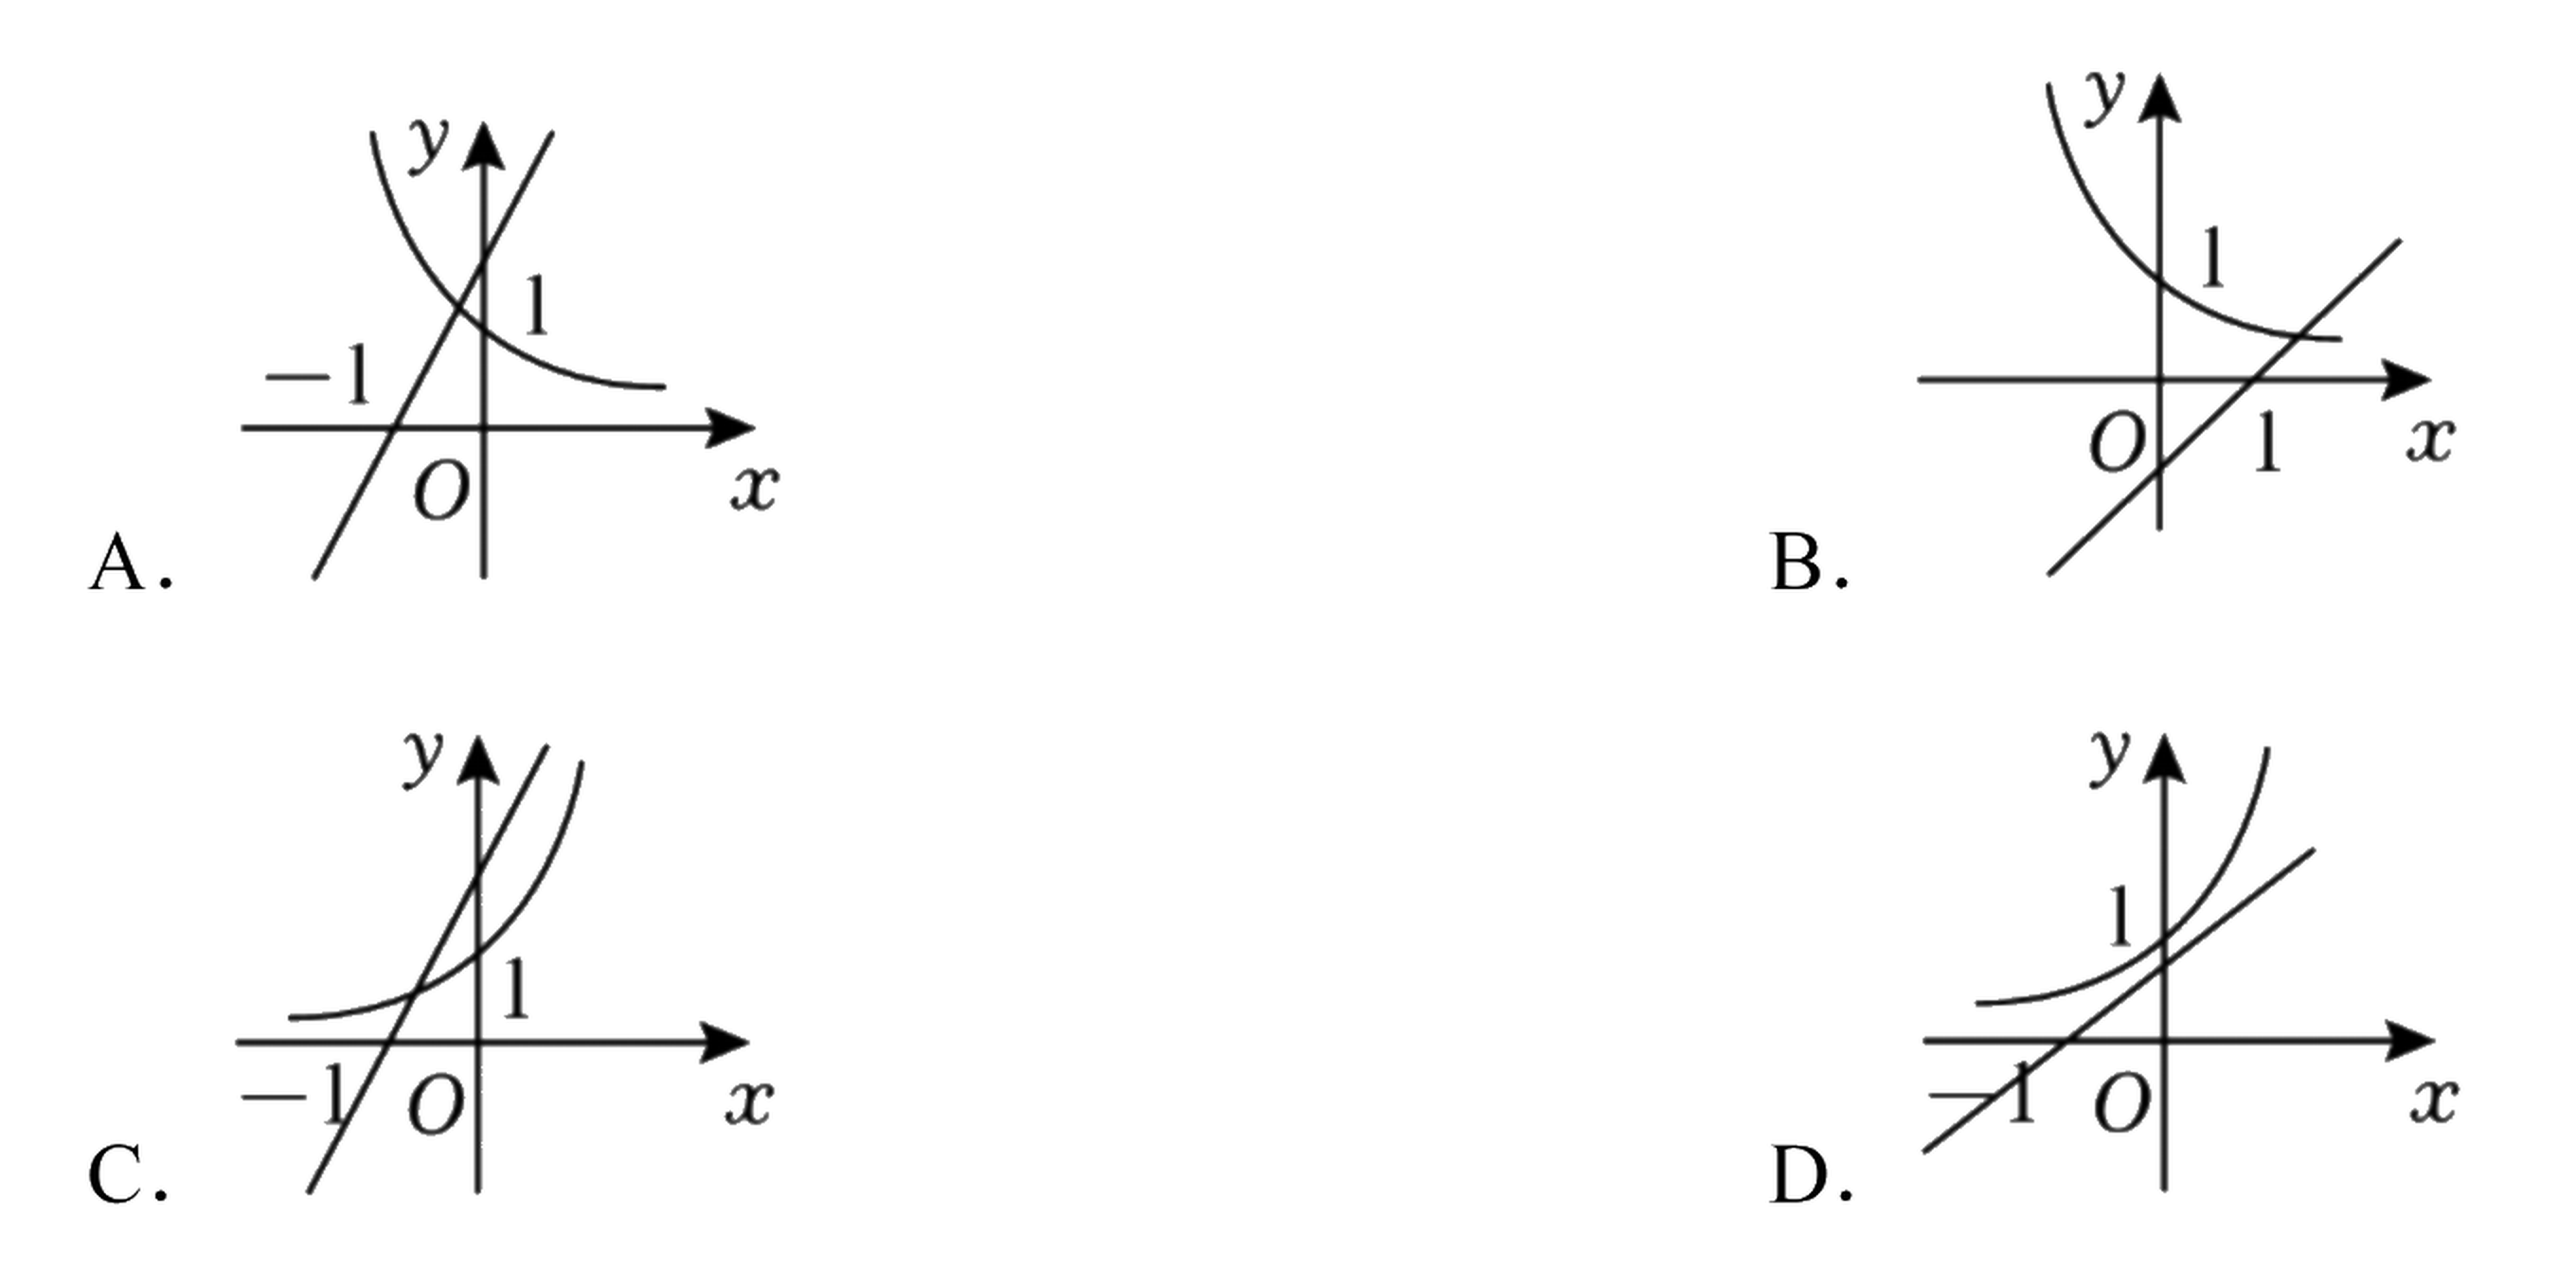
\includegraphics[width=0.80\textwidth]{figures/gao130_q15.png}
\end{center}

\ifanswer
\solbegin
\step{A 中，由指数函数 $y=a^x(a>0$ 且 $a\neq1)$ 图像递减得 $0<a<1$，}
\step{而一次函数 $y=a(x+1)$ 的图像与 $y$ 轴交点纵坐标为 $a>1$，二者矛盾，}
\step{所以 A 错；}
\step{由一次函数 $y=a(x+1)$ 的图像与 $x$ 轴交点横坐标为 $-1$，排除 B；}
\step{C 中，由指数函数 $y=a^x(a>0$ 且 $a\neq1)$ 图像递减得 $a>1$，}% 原卷"递减得 a>1"系笔误（应为"递增"），与 A 中"递减得 0<a<1"自相矛盾，照录
\step{而一次函数 $y=a(x+1)$ 的图像与 $y$ 轴交点纵坐标为 $a>1$，二者 $a$ 值吻合，}
\step{所以 C 对；}
\step{D 中，由一次函数 $y=a(x+1)$ 的图像得 $a=1$，与 $a>0$ 且 $a\neq1$ 矛盾，}
\step{所以 D 错.}
\step{故选 $C$.}
\solend
\fi

\item 设 $A_1$、$A_2$、$A_3$、$\cdots$、$A_7$ 是均含有 $2$ 个元素的集合，且 $A_1\cap A_7=\varnothing$，$A_i\cap A_{i+1}=\varnothing(i=1,2,3,\cdots,6)$，记 $B=A_1\cup A_2\cup A_3\cup\cdots\cup A_7$，则 $B$ 中元素个数的最小值是\mbox{（\quad）}

\keepwithprev
A. $4$\qquad B. $5$\qquad C. $6$\qquad D. $7$

\ifanswer
\solbegin
\step{取 $A_1=\{1,2\}$，$A_2=\{3,4\}$，$A_3=\{1,2\}$，$A_4=\{3,4\}$，$A_5=\{1,5\}$，$A_6=\{2,3\}$，$A_7=\{4,5\}$，}
\step{所以 $B$ 中元素个数的最小值是 $5$，故选 $B$.}
\solend
\fi

\end{enumerate}

\bigsec{三、解答题}

\begin{enumerate}
\setcounter{enumi}{16}

\item 已知全集为 $\R$，集合 $A=\{x\mid-2\leqslant x\leqslant5\}$，集合 $B=\{x\mid m-1\leqslant x\leqslant2m+1\}$．

(1) 求 $\overline{A}$；

(2) 若 $A\cup B=A$，求实数 $m$ 的取值范围．

\ifanswer
\solbegin
\step{(1) $(-\infty,-2)\cup(5,+\infty)$；}
\step{(2) 若 $A\cup B=A$，则 $B\subseteq A$，}
\step{当 $B=\varnothing$ 时，$m-1>2m+1$，解得 $m<-2$；}
\step{当 $B\neq\varnothing$ 时，$\begin{cases}m-1\leqslant2m+1\\m-1\geqslant-2\\2m+1\leqslant5\end{cases}$，解得 $-1\leqslant m\leqslant2$；}
\step{故实数 $m$ 的取值范围为 $\{m\mid-1\leqslant m\leqslant2$ 或 $m<-2\}$.}
\solend
\fi

\item 在不等式的应用中，有一些很基本而十分重要的不等式，如平均值不等式和三角不等式等，我们将其统称为基本不等式．

(1) 已知 $x$、$y$ 为正数，且 $2x+y=2$，求 $\dfrac1x+\dfrac2y$ 的最小值；

(2) 若关于 $x$ 的不等式 $\lvert x+1\rvert+\lvert2-x\rvert\geqslant a^2+a+1$ 对于一切实数 $x$ 都成立，求实数 $a$ 的取值范围．

\ifanswer
\solbegin
\step{(1) 因为 $x$、$y$ 为正数，且 $2x+y=2$，}
\step{所以 $\dfrac1x+\dfrac2y=\dfrac12\left(\dfrac1x+\dfrac2y\right)(2x+y)=\dfrac12\left(4+\dfrac yx+\dfrac{4x}y\right)\geqslant\dfrac12\left(4+2\sqrt{\dfrac yx\cdot\dfrac{4x}y}\right)=4$，}
\step{当且仅当 $\dfrac yx=\dfrac{4x}y$，即 $x=\dfrac12$，$y=1$ 时取等号，所以 $\dfrac1x+\dfrac2y$ 的最小值为 $4$；}
\step{(2) 由绝对值三角不等式得 $\lvert x+1\rvert+\lvert2-x\rvert\geqslant\lvert(x+1)+(2-x)\rvert=3$，}
\step{当且仅当 $-1\leqslant x\leqslant2$ 时取等号，所以 $\lvert x+1\rvert+\lvert2-x\rvert$ 的最小值为 $3$，}
\step{因为关于 $x$ 的不等式 $\lvert x+1\rvert+\lvert2-x\rvert\geqslant a^2+a+1$ 对于一切实数 $x$ 都成立，}
\step{所以 $a^2+a+1\leqslant3$，即 $a^2+a-2\leqslant0$，解得 $-2\leqslant a\leqslant1$，}
\step{所以实数 $a$ 的取值范围是 $[-2,1]$.}
\solend
\fi

\item 某医学专家为研究传染病传播中病毒细胞的发展规律，将病毒细胞注入一只小白鼠体内进行试验，经检测，病毒细胞的个数 $y$ 与天数 $x$ 的部分数据如表所示：

\begin{center}
\begin{tabular}{|c|c|c|c|c|c|c|c|}
\hline
天数 $(x)$ & $1$ & $2$ & $3$ & $4$ & $5$ & $6$ & $\cdots$ \\
\hline
病毒细胞的个数 $(y)$ & $1$ & $2$ & $4$ & $8$ & $16$ & $32$ & $\cdots$ \\
\hline
\end{tabular}
\end{center}

(1) 若病毒细胞的个数 $y$ 关于天数 $x$ 的变化规律可选用以下两个函数模型之一进行近似刻画：① $y=a\cdot b^x(a>0$，$b>0$，$b\neq1)$；② $y=a\cdot x^k(a\neq0)$．请结合表格中的数据，选择合适的函数模型，说明理由，并求出相应的函数表达式；

(2) 若该病毒细胞在小白鼠体内的个数超过 $10^8$，小白鼠将死亡，但注射某种药物，可杀死其体内 $98\%$ 的病毒细胞．则在 (1) 的条件下，为了使小白鼠在试验过程中不死亡，第一次最迟应在何时注射该种药物？（结果精确到天）

\ifanswer
\solbegin
\step{(1) 选择模型① $y=a\cdot b^x(a>0$，$b>0$，$b\neq1)$，理由如下：}
\step{观察表格数据，$y$ 的值随 $x$ 呈指数倍增：}
\step{$x=1$ 时，$y=1$，$x=2$ 时，$y=2$，$x=3$ 时，$y=4$，}
\step{后一天的病毒数是前一天的 $2$ 倍，符合指数增长的特征；}
\step{若选用幂函数模型 $y=a\cdot x^k$，代入前两组数据得 $a\cdot1^k=1$、$a\cdot2^k=2$，}
\step{解得 $a=1$，$k=1$，即 $y=x$，}
\step{但 $x=3$ 时，$y=3$ 与表格中 $y=4$ 严重不符，因此幂函数不匹配；}
\step{将 $(1,1)$ 代入 $y=a\cdot b^x$ 得 $a\cdot b=1$，}
\step{将 $(2,2)$ 代入得 $a\cdot b^2=2$，两式相除得 $b=2$，进而得 $a=\dfrac12$，}
\step{验证所有表格点均满足 $y=2^{x-1}$，最终函数表达式为 $y=2^{x-1}(x\in\N^*)$；}
\step{(2) 由题意得第一次注射药物前病毒细胞个数 $y$ 关于天数 $x(x\in\N^*)$ 的函数}
\step{关系式为 $y=2^{x-1}(x\in\N^*)$，}
\step{为了使小白鼠在试验过程中不死亡，则 $2^{x-1}\leqslant10^8$，}
\step{所以 $x-1\leqslant\log_210^8=8\log_210=\dfrac8{\lg2}$，解得 $x\leqslant1+\dfrac8{\lg2}\approx27.6$，}
\step{又 $x\in\N^*$，所以第一次最迟应在第 $27$ 天注射该种药物.}
\solend
\fi

\item 对在直角坐标系的第一象限内的任意两点 $(a,b)$，$(c,d)$ 作如下定义：$\dfrac ab>\dfrac cd$，那么称点 $(a,b)$ 是点 $(c,d)$ 的“上位点”，同时点 $(c,d)$ 是点 $(a,b)$ 的“下位点”．

(1) 试写出点 $(3,5)$ 的一个“上位点”坐标和一个“下位点”坐标；

(2) 设 $a$、$b$、$c$、$d$ 均为正数，且点 $(a,b)$ 是点 $(c,d)$ 的上位点，请判断点 $P(a+c,b+d)$ 是否既是点 $(a,b)$ 的“下位点”又是点 $(c,d)$ 的“上位点”，如果是，请证明；如果不是，请说明理由；

(3) 设正整数 $n$ 满足以下条件：对任意实数 $m\in\{t\mid0<t<4,t\in\Z\}$，总存在正整数 $k$，使得点 $(n,k)$ 既是点 $(4,m)$ 的“下位点”，又是点 $(5,m+1)$ 的“上位点”，求正整数 $n$ 的最小值．

\ifanswer
\solbegin
\step{(1) 由 $\dfrac34>\dfrac35>\dfrac36$ 得点 $(3,5)$ 的一个“上位点”的坐标为 $(3,4)$，}
\step{一个“下位点”的坐标为 $(3,6)$.}
\step{(2) 是，证明如下：}
\step{因为 $a$、$b$、$c$、$d$ 均为正数，点 $(a,b)$ 是点 $(c,d)$ 的“上位点”，}
\step{所以 $\dfrac ab>\dfrac cd$，所以 $ad>bc$，}
\step{因为 $\dfrac{a+c}{b+d}-\dfrac ab=\dfrac{b(a+c)-a(b+d)}{b(b+d)}=\dfrac{bc-ad}{b(b+d)}<0$，所以 $\dfrac{a+c}{b+d}<\dfrac ab$，}
\step{点 $P(a+c,b+d)$ 是点 $(a,b)$ 的“下位点”，}
\step{因为 $\dfrac{a+c}{b+d}-\dfrac cd=\dfrac{d(a+c)-c(b+d)}{d(b+d)}=\dfrac{ad-bc}{d(b+d)}>0$.}
\step{所以 $\dfrac{a+c}{b+d}>\dfrac cd$ 点 $P(a+c,b+d)$ 是点 $(c,d)$ 的“上位点”；}
\step{所以 $P(a+c,b+d)$ 既是点 $(a,b)$ 的“下位点”又是点 $(c,d)$ 的“上位点”；}
\step{(3) 由题意得 $m=1,2,3$，}
\step{由题意存在正整数 $k$：$\dfrac5{m+1}<\dfrac nk<\dfrac4m$，所以 $\begin{cases}\dfrac n4<k<\dfrac{2n}5(m=1)\\\dfrac n2<k<\dfrac{3n}5(m=2)\\\dfrac{3n}4<k<\dfrac{4n}5(m=3)\end{cases}$，}
\step{检验：$n=1,2,\cdots,8$ 不能同时找到整数 $k$，}
\step{$n=9$：$m=1$ 取 $k=3$，$m=2$ 取 $k=5$，$m=3$ 取 $k=7$，均满足，}
\step{所以正整数 $n$ 的最小值为 $9$.}
\solend
\fi

\end{enumerate}

\end{document}
"
% 紧凑版：xelatex "\def\iscompact{1}% 高一130_北郊高级中学_期中.tex
%   —— 高一上数学"2026-2027 年北郊高级中学高一上期中"（试卷版/答案版）
% 试卷版：xelatex 高一130_北郊高级中学_期中.tex
% 答案版：xelatex "\def\isanswer{1}\input{高一130_北郊高级中学_期中.tex}"
% 紧凑版：xelatex "\def\iscompact{1}\input{高一130_北郊高级中学_期中.tex}"
%
% ① 原始材料：微信公众号"魔都数学加油站"文章，连载"27学年高一140"，原文标题
% "27学年高一140——2026-2027年上海市北郊高级中学高一上期中"；
% 原文链接：https://mp.weixin.qq.com/s/XBEYuTheiBoqu15dtLuD6A。
%   ★ 编号不一致说明：公众号连载号印"140"，与上一批已入库的"高一140 甘泉外国语"
%   （同一公众号另一篇文章、同为期中卷）撞号，系公众号笔误/重复。本仓库数字编号
%   02—143 中"高一130"一直空缺（连载 130 暂未见原文），故将本卷本地编号定为"高一130"、
%   填补该空缺，使数字编号连续（basename 全程为 高一130_北郊高级中学_期中）；
%   连载号 143 归正牌卷"上海中学 高一上期中"；本卷连载号仍印 140，见材料流转表。
%   卷面标题印"2026-2027 年北郊高级中学高一上期中"（卷面只有学校名、不含"上海市"、
%   不含任何期号/连载号），本稿照卷面录入；粉红色水印"魔都数学加油站"及页脚未录入。
% 正文为 9 张 PNG 页（01、04、05、06、09 为 2560x3620；02、03、07、08 为 4762x6735，
% 同一篇各页分辨率不同，逐页按各自分辨率放大核对），题目下印有【解析】，为讲评版。
% 题目、解析均据原图转录。
%
% 卷首标题：原卷印作"2026-2027 年北郊高级中学高一上期中"，年份区间按全稿惯例排
% en dash；原卷未印副标题，本卷为期中卷、跨集合与常用逻辑用语／不等式／函数三章，
% 按题目内容补出"集合与常用逻辑用语、不等式、函数"（与 125／126／128／129／131／132／133
% 同期中卷口径相同）。
%
% 题号体例：本卷共 18 题——一、填空题 3—12（10 题）、二、选择题 13—16（4 题）、
% 三、解答题 17—20（4 题）。三节分别 \setcounter{enumi}{2}／{12}／{16}。
% 原卷从第 3 题起、无第 1、2 题、**无第 21 题**（第 20 题解析续至 09 页，末行
% "所以正整数 n 的最小值为 9."，09 页下半页整片空白＋水印收尾、无第 10 页），本稿保留原题号。
%
% ② 与原卷的排版差异：
%   ① 原文从第 3 题起，本稿保留原题号；原卷止于第 20 题、无第 21 题、无附加题节；
%   ② 原卷每题下直接印【解析】，本稿按全稿惯例置于答案版；全卷 18 题均印【解析】、
%      无独立【答案】段，四道选择题答案在解析末句"故选 C／D／C／B"，括号
%      \mbox{（\quad）} 留空、不另提 \ans{}；全卷 0 处 \ans{}，答案版【解析】标记数 18＝题数；
%   ③ 原卷未印副标题，本稿按"知识模块"口径补出；
%   ④ 原卷填空横线按全稿惯例排为 \blankline[4.4em]；选择题括号排 \mbox{（\quad）}、
%      每个选项段前按惯例加 \keepwithprev；解答题不留作答区、不加 \anspace（讲评版）；
%   ⑤ 原卷数集排斜体 $R$／$N$，按全稿惯例改 \R／\N；空集记号 \varnothing；
%      绝对值排 \lvert…\rvert，集合描述竖线排 \mid；不等号按全稿惯例排 \leqslant／\geqslant；
%      补集照原卷上划线 \overline{A}；
%   ⑥ 1 幅插图 + 1 张印刷表格：第 15 题四幅坐标函数图象选项（04 页）取原卷截图
%      去粉色水印、去色、按原卷 2x2 排布合并为 figures/gao130_q15.png（非插图重绘），
%      放在 \keepwithprev 之后 \begin{center} 内、三版都出；第 19 题 (1) 印刷数据表格
%      （07 页，天数 x 1—6／病毒细胞个数 y 1/2/4/8/16/32）按原卷用 tabular 重排、
%      题干内三版都出（非插图）。
%      第 15 题是"二、选择题"节内带大图块的第三题（Q13 为节首题但无图），
%      在 \bigsec{二、选择题} 之前加 \needvspace{11cm} 连节标题一起量、Q15 \item 之前
%      加 \needvspace{9cm}——守卫必须放在 \bigsec 之前，放标题之后会让"二、选择题"
%      孤立在页末（B 类，照 高一26／40／59／136／140 成例）；三版切页审计均"合计异常：无"；
%   ⑦ 子题标号 (1)(2)(3) 原卷用半角括号，照录；圈数字 ①②③④ 照录；
%      数学式内半角逗号照录（如第 14 题 $(a>0,a\neq1)$、第 16 题
%      $(i=1,2,3,\cdots,6)$、第 20 题 $m=1,2,3$ 等）；
%      行末西文句点按全稿惯例照录；
%   ⑧ 题干中的中文弯引号按原卷照录（Q12"变项和"、Q20"上位点""下位点"等），
%      注释内一律 ASCII 引号；原卷"图像"用词逐处照录（Q9、Q15 均作"图像"）。
%
% ③ 行数复核：一条 \step = 原卷解析的一个印刷行（cases 块与 tabular 各作一个印刷行计）。
%   逐题 \step 条数，合计 98 条（Q3:3 Q4:2 Q5:2 Q6:1 Q7:1 Q8:3 Q9:5 Q10:10 Q11:6
%   Q12:7 Q13:1 Q14:2 Q15:10 Q16:2 Q17:5 Q18:8 Q19:15 Q20:15），与原卷印刷行逐题相等。
%
% ④ 判别式／子集符号结论：
%   判别式：全卷未出现判别式记号（无 $\Delta$、无 $\triangle$）；
%   子集符号：第 4 题题干"$B\subseteq A$"、第 4 题【解析】"$B\subseteq A$"、
%      第 17 题 (2)【解析】"$B\subseteq A$"三处原卷均印带下划线 $\subseteq$，逐处
%      放大核对、照录 \subseteq；全卷未出现单线 \subset。
%
% ⑤ 原卷存疑照录（均照录未改，正文对应处另有 % 注）：
%   ① 第 15 题【解析】"C 中，由指数函数 $y=a^x$ 图像递减得 $a>1$"——"递减"应为
%      "递增"之误（与同题 A 中"递减得 $0<a<1$"自相矛盾），原卷如此，照录并加注；
%   ② 第 16 题题干"$A_1\cap A_7=\varnothing$""$A_i\cap A_{i+1}=\varnothing$"
%      的空集记号与解析所列各集合逐处照录；
%   ③ 第 19 题 (2) 题干"可杀死其体内 98% 的病毒细胞"、解析 (2) 只按 $y=2^{x-1}$
%      与 $10^8$ 比较（未另计 98%），照录不补步。
%
% ⑥ 跨页续印按题合并：Q8 题干在 01 页末、解析在 02 页；Q9 题干在 02 页、
%   解析在 02 页；Q10 题干在 02 页、解析前 5 行在 02—03 页、后 5 行在 03 页；
%   Q12 题干跨 03 页、解析首 5 行在 03 页末、末行在 04 页；Q15 题干在 04 页、
%   四幅图与解析前段在 04 页、解析续在 05 页；Q17 解析跨 05—06 页；Q18 题干与
%   (1) 解析在 06 页、(2) 解析在 06—07 页；Q19 表格在 07 页、解析跨 07—08 页；
%   Q20 定义与三小问在 08 页、解析 (1)(2) 在 08—09 页、解析 (3) 在 09 页；
%   本稿按题连排，不丢行。
%
\documentclass[a4paper,11pt]{article}
\usepackage{common}

\begin{document}

\examtitlest[3]{2026--2027 年北郊高级中学高一上期中}{集合与常用逻辑用语、不等式、函数}

\bigsec{一、填空题}

\begin{enumerate}
\setcounter{enumi}{2}

\item 不等式 $\dfrac{x-3}{x+1}<2$ 的解集为\blankline[4.4em].

\ifanswer
\solbegin
\step{不等式 $\dfrac{x-3}{x+1}<2$ 可化为 $\dfrac{x-3}{x+1}-2<0$，即 $\dfrac{x-3-2(x+1)}{x+1}<0$，}
\step{化简为 $\dfrac{x+5}{x+1}>0$，解得 $x<-5$ 或 $x>-1$，}
\step{所以不等式的解集为 $\{x\mid x<-5$ 或 $x>-1\}$.}
\solend
\fi

\item 已知集合 $A=\{x\mid0<x<a\}$，$B=\{x\mid1<x<2\}$，若 $B\subseteq A$，则实数 $a$ 的取值范围为\blankline[4.4em].

\ifanswer
\solbegin
\step{已知集合 $A=\{x\mid0<x<a\}$，$B=\{x\mid1<x<2\}$，}
\step{若 $B\subseteq A$，则 $a\geqslant2$，所以实数 $a$ 的取值范围是 $\{a\mid a\geqslant2\}$.}
\solend
\fi

\item 已知关于 $x$ 的方程 $x^2+x+c=0$ 的两个实数根为 $x_1$、$x_2$，若 $x_1^2x_2+x_2^2x_1=3$，则实数 $c=$\blankline[4.4em].

\ifanswer
\solbegin
\step{由韦达定理得 $x_1+x_2=-1$，$x_1x_2=c$，所以 $x_1^2x_2+x_2^2x_1=(x_1+x_2)x_1x_2=-c=3$，}
\step{所以 $c=-3$.}
\solend
\fi

\item 已知 $10^x=3$，$10^y=64$，则 $10^{x-\frac y3}=$\blankline[4.4em].

\ifanswer
\solbegin
\step{$10^{x-\frac y3}=10^x\div\sqrt[3]{10^y}=\dfrac34$.}
\solend
\fi

\item 若 $\lg2=a$，则可用 $a$ 表示 $\log_280=$\blankline[4.4em].

\ifanswer
\solbegin
\step{$\log_280=\dfrac{\lg80}{\lg2}=\dfrac{\lg10+\lg8}{\lg2}=\dfrac{1+3\lg2}{\lg2}=\dfrac{1+3a}{a}$.}
\solend
\fi

\item 已知 $a+2b=1$，则 $3^a+9^b$ 的最小值为\blankline[4.4em].

\ifanswer
\solbegin
\step{因为 $a+2b=1$，所以 $3^a+9^b=3^a+3^{2b}\geqslant2\sqrt{3^a\cdot3^{2b}}=2\sqrt{3^{a+2b}}=2\sqrt3$，}
\step{当且仅当 $3^a=3^{2b}$，且 $a+2b=1$，即 $a=\dfrac12$，$b=\dfrac14$ 时取等号，}
\step{故最小值为 $2\sqrt3$.}
\solend
\fi

\item 下列函数的图像关于原点成中心对称，且在区间 $(0,+\infty)$ 上是严格增函数的是\blankline[4.4em]（请填写全部正确的序号）.

① $y=\sqrt{x}$；② $y=\sqrt[3]{x}$；③ $y=x^{\frac23}$；④ $y=x^{-\frac13}$.

\ifanswer
\solbegin
\step{① $y=\sqrt{x}$ 的定义域为 $[0,+\infty)$，故其图像不关于原点成中心对称，①错误；}
\step{② $y=\sqrt[3]{x}$ 是奇函数，且在区间 $(0,+\infty)$ 上是严格增函数，②正确；}
\step{③ $y=x^{\frac23}$ 是偶函数，其图像关于 $y$ 轴对称，不关于原点成中心对称，③错误；}
\step{④由于幂指数 $-\dfrac13<0$，故 $y=x^{-\frac13}$ 在区间 $(0,+\infty)$ 上是严格减函数，④错误.}
\step{故正确的是②.}
\solend
\fi

\item 设 $a>0$ 且 $a\neq1$，若函数 $y=a^{2x}+2a^x-3$ 在区间 $[-1,1]$ 上的最大值为 $21$，则实数 $a$ 的值为\blankline[4.4em].

\ifanswer
\solbegin
\step{令 $t=a^x$，$x\in[-1,1]$，}
\step{当 $a>1$ 时，$t=a^x$ 严格增，则 $t\in\left[\dfrac1a,a\right]$，}
\step{则函数 $y=t^2+2t-3$，对称轴为 $t=-1$，}
\step{所以函数 $y=t^2+2t-3$ 在 $\left[\dfrac1a,a\right]$ 上严格增，}
\step{所以当 $t=a$ 时，$y$ 取得最大值 $a^2+2a-3=21$，解得 $a=4$ 或 $-6$（舍去）；}
\step{当 $0<a<1$ 时，$t=a^x$ 严格减，则 $t\in\left[a,\dfrac1a\right]$，}
\step{则函数 $y=t^2+2t-3$，对称轴为 $t=-1$，}
\step{所以函数 $y=t^2+2t-3$ 在 $\left[a,\dfrac1a\right]$ 上严格增，}
\step{所以当 $t=\dfrac1a$ 时，$y$ 取得最大值 $\dfrac1{a^2}+\dfrac2a-3=21$，解得 $a=\dfrac14$ 或 $-\dfrac16$（舍去）；}
\step{综上所述，实数 $a$ 的值为 $4$ 或 $\dfrac14$.}
\solend
\fi

\item 在关于 $x$ 的不等式 $x^2+(m+1)x+m<0$ 的解集中恰有两个整数，则实数 $m$ 的取值范围是\blankline[4.4em].

\ifanswer
\solbegin
\step{关于 $x$ 的不等式 $x^2+(m+1)x+m<0$ 可化为 $(x+1)(x+m)<0$，}
\step{当 $m>1$ 时，$-m<-1$，解不等式得 $-m<x<-1$；}
\step{当 $m<1$ 时，$-m>-1$，解不等式得 $-1<x<-m$；}
\step{由不等式的解集中恰有两个整数，}
\step{则 $-4\leqslant-m<-3$ 或 $1<-m\leqslant2$，即 $3<m\leqslant4$ 或 $-2\leqslant m<-1$，}
\step{所以 $m$ 的取值范围是 $[-2,-1)\cup(3,4]$.}
\solend
\fi

\item 已知集合 $M$ 的元素均为正整数，定义集合 $M$ 的“变项和”为：将 $M$ 中每个元素 $m$ 都乘以 $(-1)^m$ 后再求和．若集合 $A=\{n\mid1\leqslant n\leqslant20,n\in\N\}$，则集合 $A$ 的所有非空子集的“变项和”的总和为\blankline[4.4em].

\ifanswer
\solbegin
\step{集合 $A=\{n\mid1\leqslant n\leqslant20,n\in\N\}$ 中一共有 $20$ 个元素，}
\step{固定选中 $k$，剩下 $19$ 个元素任选，共 $2^{19}$ 个子集包含 $k$，每个 $k$ 贡献 $(-1)^k\cdot k\cdot2^{19}$，}
\step{$A=\{1,2,\cdots,20\}$，}
\step{奇数 $k=1,3,\cdots,19$，共 $10$ 个，$(-1)^k\cdot k=-k$，}
\step{偶数 $k=2,4,\cdots,20$，共 $10$ 个，$(-1)^k\cdot k=k$，}
\step{所以集合 $A$ 的所有非空子集的“变项和”的总和}
\step{为 $S=2^{19}\times[(-1+2)+(-3+4)+\cdots+(-19+20)]=2^{19}\times10=524880$.}
\solend
\fi

\end{enumerate}

% 第 15 题四幅图是"二、选择题"节内大图块；守卫须放在 \bigsec 之前连节标题一起量，
% 否则"二、选择题"会孤立在页末（B 类，照 高一26／40／59／136／140 成例）
\needvspace{11cm}
\bigsec{二、选择题}

\begin{enumerate}
\setcounter{enumi}{12}

\item 设 $ab>0$，则“$a>b$”是“$\dfrac1a<\dfrac1b$”的\mbox{（\quad）}

\keepwithprev
A. 充分非必要条件\qquad B. 必要非充分条件

C. 充要条件\qquad D. 既非充分也非必要条件

\ifanswer
\solbegin
\step{因为 $ab>0$，所以 $a>b\Leftrightarrow\dfrac1a<\dfrac1b$，故选 $C$.}
\solend
\fi

\item 已知 $A=\log_ax$，$B=\log_ay(a>0,a\neq1)$，则 $\log_a\dfrac{x^2}{\sqrt y}=$\mbox{（\quad）}

\keepwithprev
A. $\dfrac{A^2}{\sqrt B}$\qquad B. $2A^2B$\qquad C. $4AB$\qquad D. $2A-\dfrac12B$

\ifanswer
\solbegin
\step{由已知得 $x=a^A$，$y=a^B$，}
\step{所以 $\log_a\dfrac{x^2}{\sqrt y}=\log_a\dfrac{(a^A)^2}{\sqrt{a^B}}=\log_a\dfrac{a^{2A}}{a^{\frac12B}}=\log_a a^{2A-\frac12B}=2A-\dfrac12B$. 故选 $D$.}
\solend
\fi

% 第 15 题四幅坐标函数图象选项是一整块，守卫放在 \item 之前
\needvspace{9cm}
\item 在同一平面直角坐标系中，指数函数 $y=a^x(a>0$ 且 $a\neq1)$ 和一次函数 $y=a(x+1)$ 的图像关系可能是\mbox{（\quad）}

\keepwithprev
\begin{center}
% 四幅坐标函数图象选项取原卷 04 页截图去粉色水印、去色，按原卷 2x2 排布合并为一张
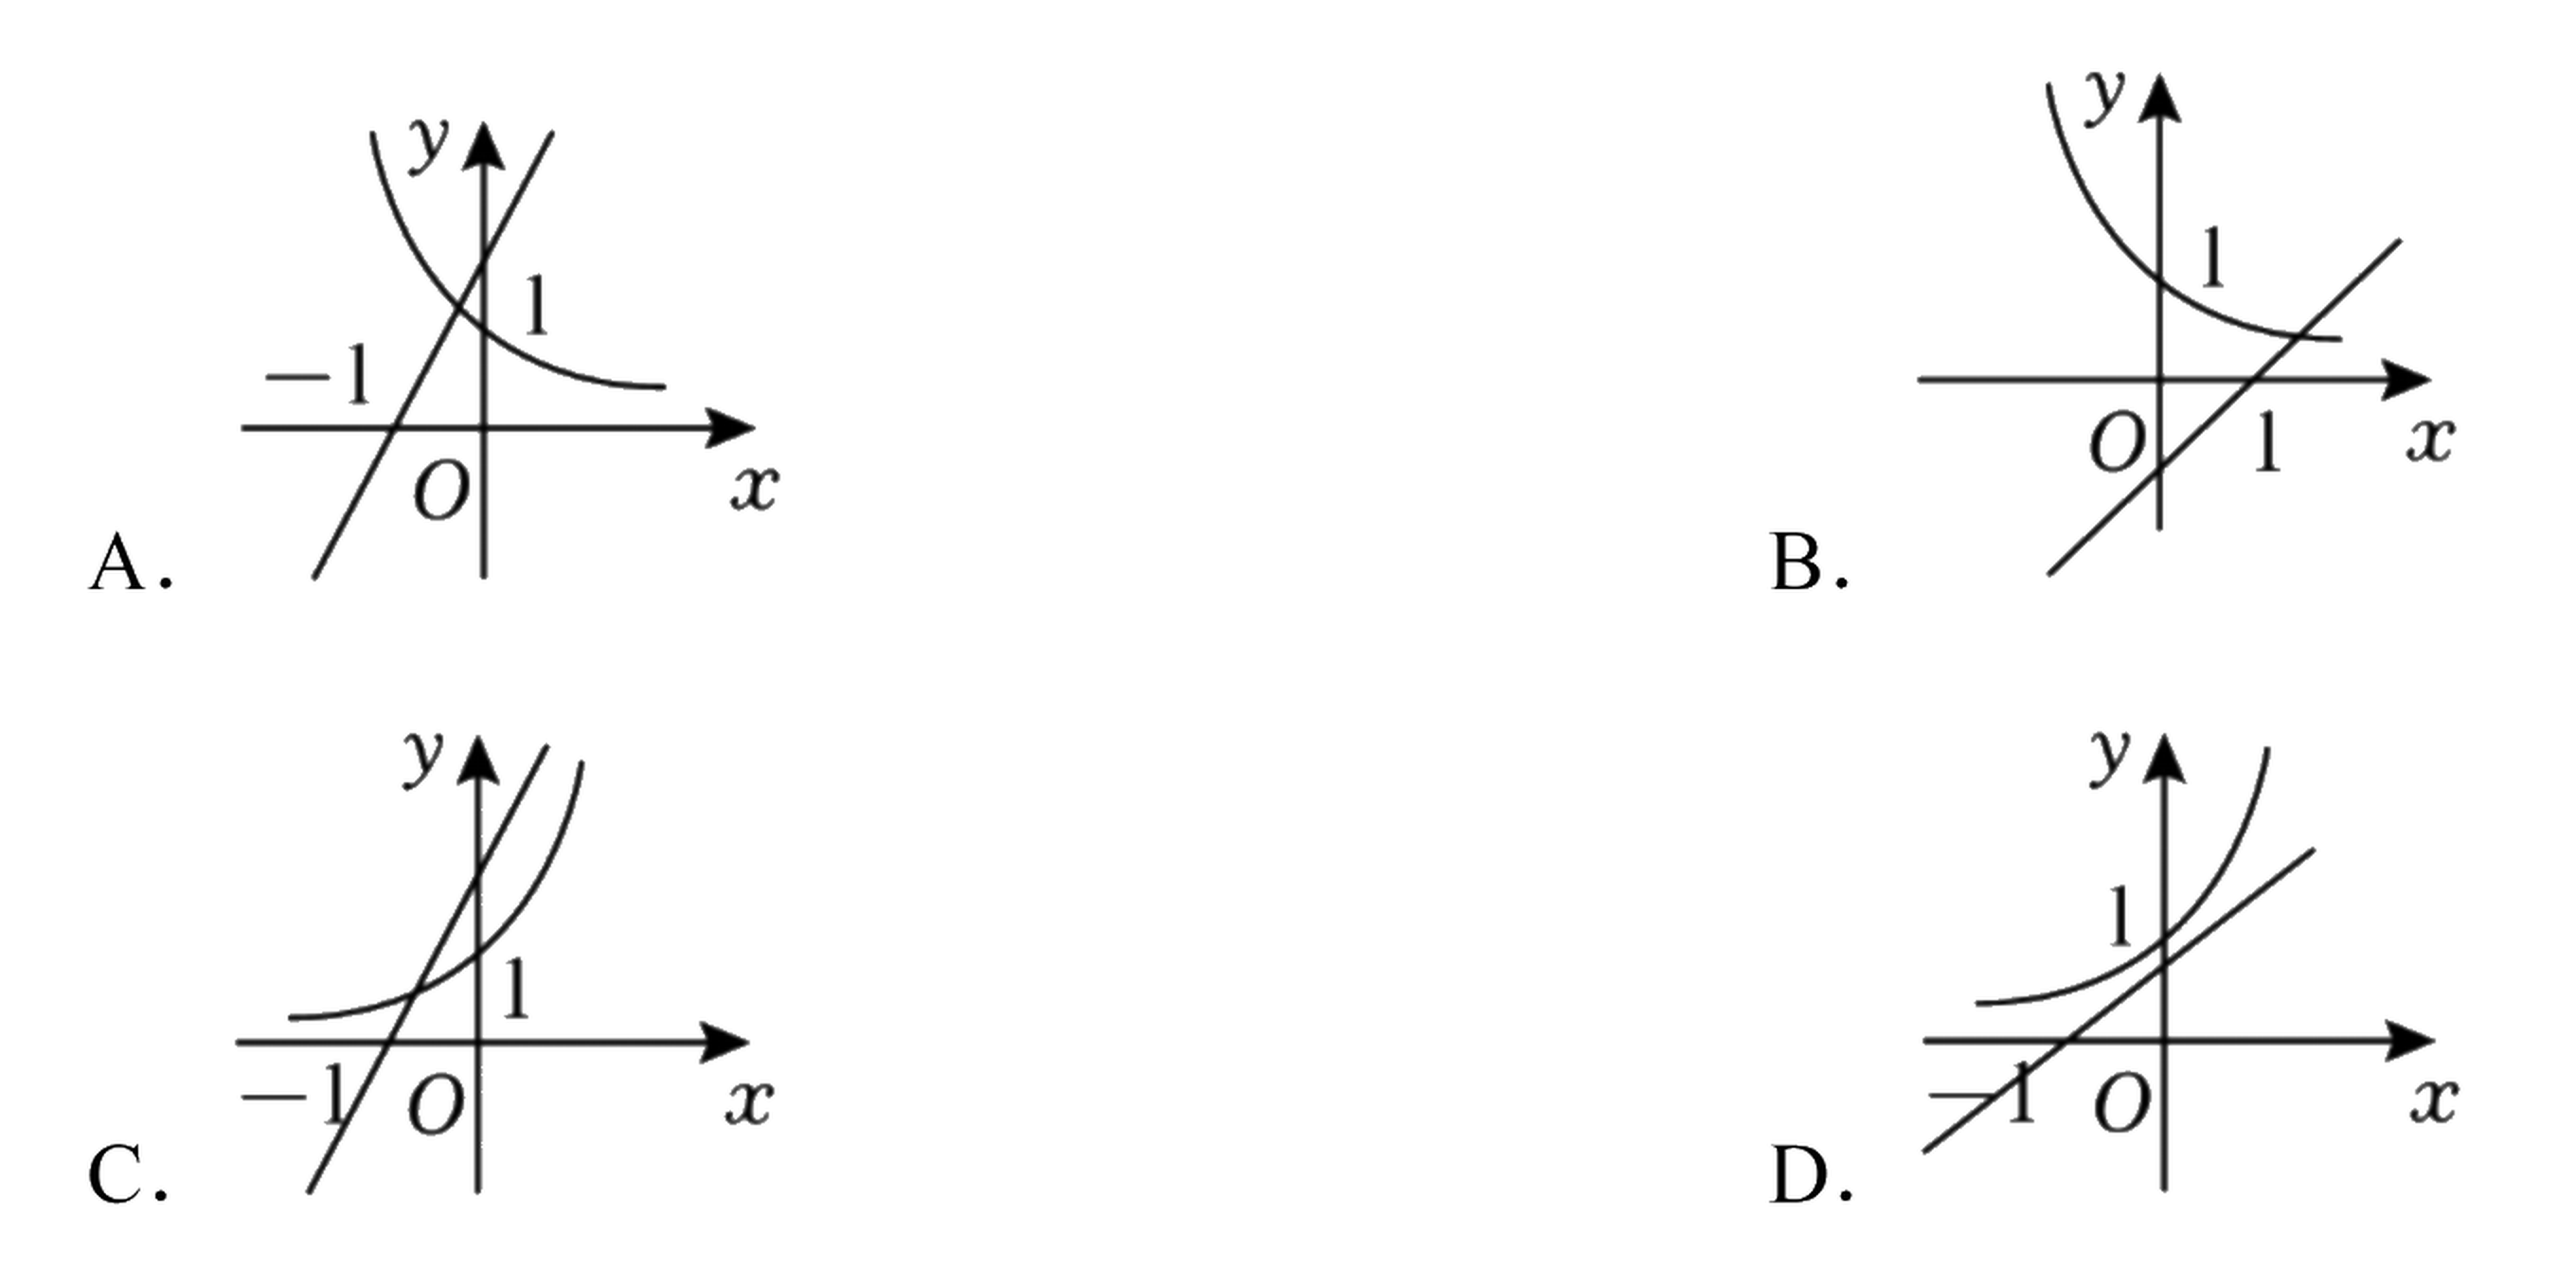
\includegraphics[width=0.80\textwidth]{figures/gao130_q15.png}
\end{center}

\ifanswer
\solbegin
\step{A 中，由指数函数 $y=a^x(a>0$ 且 $a\neq1)$ 图像递减得 $0<a<1$，}
\step{而一次函数 $y=a(x+1)$ 的图像与 $y$ 轴交点纵坐标为 $a>1$，二者矛盾，}
\step{所以 A 错；}
\step{由一次函数 $y=a(x+1)$ 的图像与 $x$ 轴交点横坐标为 $-1$，排除 B；}
\step{C 中，由指数函数 $y=a^x(a>0$ 且 $a\neq1)$ 图像递减得 $a>1$，}% 原卷"递减得 a>1"系笔误（应为"递增"），与 A 中"递减得 0<a<1"自相矛盾，照录
\step{而一次函数 $y=a(x+1)$ 的图像与 $y$ 轴交点纵坐标为 $a>1$，二者 $a$ 值吻合，}
\step{所以 C 对；}
\step{D 中，由一次函数 $y=a(x+1)$ 的图像得 $a=1$，与 $a>0$ 且 $a\neq1$ 矛盾，}
\step{所以 D 错.}
\step{故选 $C$.}
\solend
\fi

\item 设 $A_1$、$A_2$、$A_3$、$\cdots$、$A_7$ 是均含有 $2$ 个元素的集合，且 $A_1\cap A_7=\varnothing$，$A_i\cap A_{i+1}=\varnothing(i=1,2,3,\cdots,6)$，记 $B=A_1\cup A_2\cup A_3\cup\cdots\cup A_7$，则 $B$ 中元素个数的最小值是\mbox{（\quad）}

\keepwithprev
A. $4$\qquad B. $5$\qquad C. $6$\qquad D. $7$

\ifanswer
\solbegin
\step{取 $A_1=\{1,2\}$，$A_2=\{3,4\}$，$A_3=\{1,2\}$，$A_4=\{3,4\}$，$A_5=\{1,5\}$，$A_6=\{2,3\}$，$A_7=\{4,5\}$，}
\step{所以 $B$ 中元素个数的最小值是 $5$，故选 $B$.}
\solend
\fi

\end{enumerate}

\bigsec{三、解答题}

\begin{enumerate}
\setcounter{enumi}{16}

\item 已知全集为 $\R$，集合 $A=\{x\mid-2\leqslant x\leqslant5\}$，集合 $B=\{x\mid m-1\leqslant x\leqslant2m+1\}$．

(1) 求 $\overline{A}$；

(2) 若 $A\cup B=A$，求实数 $m$ 的取值范围．

\ifanswer
\solbegin
\step{(1) $(-\infty,-2)\cup(5,+\infty)$；}
\step{(2) 若 $A\cup B=A$，则 $B\subseteq A$，}
\step{当 $B=\varnothing$ 时，$m-1>2m+1$，解得 $m<-2$；}
\step{当 $B\neq\varnothing$ 时，$\begin{cases}m-1\leqslant2m+1\\m-1\geqslant-2\\2m+1\leqslant5\end{cases}$，解得 $-1\leqslant m\leqslant2$；}
\step{故实数 $m$ 的取值范围为 $\{m\mid-1\leqslant m\leqslant2$ 或 $m<-2\}$.}
\solend
\fi

\item 在不等式的应用中，有一些很基本而十分重要的不等式，如平均值不等式和三角不等式等，我们将其统称为基本不等式．

(1) 已知 $x$、$y$ 为正数，且 $2x+y=2$，求 $\dfrac1x+\dfrac2y$ 的最小值；

(2) 若关于 $x$ 的不等式 $\lvert x+1\rvert+\lvert2-x\rvert\geqslant a^2+a+1$ 对于一切实数 $x$ 都成立，求实数 $a$ 的取值范围．

\ifanswer
\solbegin
\step{(1) 因为 $x$、$y$ 为正数，且 $2x+y=2$，}
\step{所以 $\dfrac1x+\dfrac2y=\dfrac12\left(\dfrac1x+\dfrac2y\right)(2x+y)=\dfrac12\left(4+\dfrac yx+\dfrac{4x}y\right)\geqslant\dfrac12\left(4+2\sqrt{\dfrac yx\cdot\dfrac{4x}y}\right)=4$，}
\step{当且仅当 $\dfrac yx=\dfrac{4x}y$，即 $x=\dfrac12$，$y=1$ 时取等号，所以 $\dfrac1x+\dfrac2y$ 的最小值为 $4$；}
\step{(2) 由绝对值三角不等式得 $\lvert x+1\rvert+\lvert2-x\rvert\geqslant\lvert(x+1)+(2-x)\rvert=3$，}
\step{当且仅当 $-1\leqslant x\leqslant2$ 时取等号，所以 $\lvert x+1\rvert+\lvert2-x\rvert$ 的最小值为 $3$，}
\step{因为关于 $x$ 的不等式 $\lvert x+1\rvert+\lvert2-x\rvert\geqslant a^2+a+1$ 对于一切实数 $x$ 都成立，}
\step{所以 $a^2+a+1\leqslant3$，即 $a^2+a-2\leqslant0$，解得 $-2\leqslant a\leqslant1$，}
\step{所以实数 $a$ 的取值范围是 $[-2,1]$.}
\solend
\fi

\item 某医学专家为研究传染病传播中病毒细胞的发展规律，将病毒细胞注入一只小白鼠体内进行试验，经检测，病毒细胞的个数 $y$ 与天数 $x$ 的部分数据如表所示：

\begin{center}
\begin{tabular}{|c|c|c|c|c|c|c|c|}
\hline
天数 $(x)$ & $1$ & $2$ & $3$ & $4$ & $5$ & $6$ & $\cdots$ \\
\hline
病毒细胞的个数 $(y)$ & $1$ & $2$ & $4$ & $8$ & $16$ & $32$ & $\cdots$ \\
\hline
\end{tabular}
\end{center}

(1) 若病毒细胞的个数 $y$ 关于天数 $x$ 的变化规律可选用以下两个函数模型之一进行近似刻画：① $y=a\cdot b^x(a>0$，$b>0$，$b\neq1)$；② $y=a\cdot x^k(a\neq0)$．请结合表格中的数据，选择合适的函数模型，说明理由，并求出相应的函数表达式；

(2) 若该病毒细胞在小白鼠体内的个数超过 $10^8$，小白鼠将死亡，但注射某种药物，可杀死其体内 $98\%$ 的病毒细胞．则在 (1) 的条件下，为了使小白鼠在试验过程中不死亡，第一次最迟应在何时注射该种药物？（结果精确到天）

\ifanswer
\solbegin
\step{(1) 选择模型① $y=a\cdot b^x(a>0$，$b>0$，$b\neq1)$，理由如下：}
\step{观察表格数据，$y$ 的值随 $x$ 呈指数倍增：}
\step{$x=1$ 时，$y=1$，$x=2$ 时，$y=2$，$x=3$ 时，$y=4$，}
\step{后一天的病毒数是前一天的 $2$ 倍，符合指数增长的特征；}
\step{若选用幂函数模型 $y=a\cdot x^k$，代入前两组数据得 $a\cdot1^k=1$、$a\cdot2^k=2$，}
\step{解得 $a=1$，$k=1$，即 $y=x$，}
\step{但 $x=3$ 时，$y=3$ 与表格中 $y=4$ 严重不符，因此幂函数不匹配；}
\step{将 $(1,1)$ 代入 $y=a\cdot b^x$ 得 $a\cdot b=1$，}
\step{将 $(2,2)$ 代入得 $a\cdot b^2=2$，两式相除得 $b=2$，进而得 $a=\dfrac12$，}
\step{验证所有表格点均满足 $y=2^{x-1}$，最终函数表达式为 $y=2^{x-1}(x\in\N^*)$；}
\step{(2) 由题意得第一次注射药物前病毒细胞个数 $y$ 关于天数 $x(x\in\N^*)$ 的函数}
\step{关系式为 $y=2^{x-1}(x\in\N^*)$，}
\step{为了使小白鼠在试验过程中不死亡，则 $2^{x-1}\leqslant10^8$，}
\step{所以 $x-1\leqslant\log_210^8=8\log_210=\dfrac8{\lg2}$，解得 $x\leqslant1+\dfrac8{\lg2}\approx27.6$，}
\step{又 $x\in\N^*$，所以第一次最迟应在第 $27$ 天注射该种药物.}
\solend
\fi

\item 对在直角坐标系的第一象限内的任意两点 $(a,b)$，$(c,d)$ 作如下定义：$\dfrac ab>\dfrac cd$，那么称点 $(a,b)$ 是点 $(c,d)$ 的“上位点”，同时点 $(c,d)$ 是点 $(a,b)$ 的“下位点”．

(1) 试写出点 $(3,5)$ 的一个“上位点”坐标和一个“下位点”坐标；

(2) 设 $a$、$b$、$c$、$d$ 均为正数，且点 $(a,b)$ 是点 $(c,d)$ 的上位点，请判断点 $P(a+c,b+d)$ 是否既是点 $(a,b)$ 的“下位点”又是点 $(c,d)$ 的“上位点”，如果是，请证明；如果不是，请说明理由；

(3) 设正整数 $n$ 满足以下条件：对任意实数 $m\in\{t\mid0<t<4,t\in\Z\}$，总存在正整数 $k$，使得点 $(n,k)$ 既是点 $(4,m)$ 的“下位点”，又是点 $(5,m+1)$ 的“上位点”，求正整数 $n$ 的最小值．

\ifanswer
\solbegin
\step{(1) 由 $\dfrac34>\dfrac35>\dfrac36$ 得点 $(3,5)$ 的一个“上位点”的坐标为 $(3,4)$，}
\step{一个“下位点”的坐标为 $(3,6)$.}
\step{(2) 是，证明如下：}
\step{因为 $a$、$b$、$c$、$d$ 均为正数，点 $(a,b)$ 是点 $(c,d)$ 的“上位点”，}
\step{所以 $\dfrac ab>\dfrac cd$，所以 $ad>bc$，}
\step{因为 $\dfrac{a+c}{b+d}-\dfrac ab=\dfrac{b(a+c)-a(b+d)}{b(b+d)}=\dfrac{bc-ad}{b(b+d)}<0$，所以 $\dfrac{a+c}{b+d}<\dfrac ab$，}
\step{点 $P(a+c,b+d)$ 是点 $(a,b)$ 的“下位点”，}
\step{因为 $\dfrac{a+c}{b+d}-\dfrac cd=\dfrac{d(a+c)-c(b+d)}{d(b+d)}=\dfrac{ad-bc}{d(b+d)}>0$.}
\step{所以 $\dfrac{a+c}{b+d}>\dfrac cd$ 点 $P(a+c,b+d)$ 是点 $(c,d)$ 的“上位点”；}
\step{所以 $P(a+c,b+d)$ 既是点 $(a,b)$ 的“下位点”又是点 $(c,d)$ 的“上位点”；}
\step{(3) 由题意得 $m=1,2,3$，}
\step{由题意存在正整数 $k$：$\dfrac5{m+1}<\dfrac nk<\dfrac4m$，所以 $\begin{cases}\dfrac n4<k<\dfrac{2n}5(m=1)\\\dfrac n2<k<\dfrac{3n}5(m=2)\\\dfrac{3n}4<k<\dfrac{4n}5(m=3)\end{cases}$，}
\step{检验：$n=1,2,\cdots,8$ 不能同时找到整数 $k$，}
\step{$n=9$：$m=1$ 取 $k=3$，$m=2$ 取 $k=5$，$m=3$ 取 $k=7$，均满足，}
\step{所以正整数 $n$ 的最小值为 $9$.}
\solend
\fi

\end{enumerate}

\end{document}
"
%
% ① 原始材料：微信公众号"魔都数学加油站"文章，连载"27学年高一140"，原文标题
% "27学年高一140——2026-2027年上海市北郊高级中学高一上期中"；
% 原文链接：https://mp.weixin.qq.com/s/XBEYuTheiBoqu15dtLuD6A。
%   ★ 编号不一致说明：公众号连载号印"140"，与上一批已入库的"高一140 甘泉外国语"
%   （同一公众号另一篇文章、同为期中卷）撞号，系公众号笔误/重复。本仓库数字编号
%   02—143 中"高一130"一直空缺（连载 130 暂未见原文），故将本卷本地编号定为"高一130"、
%   填补该空缺，使数字编号连续（basename 全程为 高一130_北郊高级中学_期中）；
%   连载号 143 归正牌卷"上海中学 高一上期中"；本卷连载号仍印 140，见材料流转表。
%   卷面标题印"2026-2027 年北郊高级中学高一上期中"（卷面只有学校名、不含"上海市"、
%   不含任何期号/连载号），本稿照卷面录入；粉红色水印"魔都数学加油站"及页脚未录入。
% 正文为 9 张 PNG 页（01、04、05、06、09 为 2560x3620；02、03、07、08 为 4762x6735，
% 同一篇各页分辨率不同，逐页按各自分辨率放大核对），题目下印有【解析】，为讲评版。
% 题目、解析均据原图转录。
%
% 卷首标题：原卷印作"2026-2027 年北郊高级中学高一上期中"，年份区间按全稿惯例排
% en dash；原卷未印副标题，本卷为期中卷、跨集合与常用逻辑用语／不等式／函数三章，
% 按题目内容补出"集合与常用逻辑用语、不等式、函数"（与 125／126／128／129／131／132／133
% 同期中卷口径相同）。
%
% 题号体例：本卷共 18 题——一、填空题 3—12（10 题）、二、选择题 13—16（4 题）、
% 三、解答题 17—20（4 题）。三节分别 \setcounter{enumi}{2}／{12}／{16}。
% 原卷从第 3 题起、无第 1、2 题、**无第 21 题**（第 20 题解析续至 09 页，末行
% "所以正整数 n 的最小值为 9."，09 页下半页整片空白＋水印收尾、无第 10 页），本稿保留原题号。
%
% ② 与原卷的排版差异：
%   ① 原文从第 3 题起，本稿保留原题号；原卷止于第 20 题、无第 21 题、无附加题节；
%   ② 原卷每题下直接印【解析】，本稿按全稿惯例置于答案版；全卷 18 题均印【解析】、
%      无独立【答案】段，四道选择题答案在解析末句"故选 C／D／C／B"，括号
%      \mbox{（\quad）} 留空、不另提 \ans{}；全卷 0 处 \ans{}，答案版【解析】标记数 18＝题数；
%   ③ 原卷未印副标题，本稿按"知识模块"口径补出；
%   ④ 原卷填空横线按全稿惯例排为 \blankline[4.4em]；选择题括号排 \mbox{（\quad）}、
%      每个选项段前按惯例加 \keepwithprev；解答题不留作答区、不加 \anspace（讲评版）；
%   ⑤ 原卷数集排斜体 $R$／$N$，按全稿惯例改 \R／\N；空集记号 \varnothing；
%      绝对值排 \lvert…\rvert，集合描述竖线排 \mid；不等号按全稿惯例排 \leqslant／\geqslant；
%      补集照原卷上划线 \overline{A}；
%   ⑥ 1 幅插图 + 1 张印刷表格：第 15 题四幅坐标函数图象选项（04 页）取原卷截图
%      去粉色水印、去色、按原卷 2x2 排布合并为 figures/gao130_q15.png（非插图重绘），
%      放在 \keepwithprev 之后 \begin{center} 内、三版都出；第 19 题 (1) 印刷数据表格
%      （07 页，天数 x 1—6／病毒细胞个数 y 1/2/4/8/16/32）按原卷用 tabular 重排、
%      题干内三版都出（非插图）。
%      第 15 题是"二、选择题"节内带大图块的第三题（Q13 为节首题但无图），
%      在 \bigsec{二、选择题} 之前加 \needvspace{11cm} 连节标题一起量、Q15 \item 之前
%      加 \needvspace{9cm}——守卫必须放在 \bigsec 之前，放标题之后会让"二、选择题"
%      孤立在页末（B 类，照 高一26／40／59／136／140 成例）；三版切页审计均"合计异常：无"；
%   ⑦ 子题标号 (1)(2)(3) 原卷用半角括号，照录；圈数字 ①②③④ 照录；
%      数学式内半角逗号照录（如第 14 题 $(a>0,a\neq1)$、第 16 题
%      $(i=1,2,3,\cdots,6)$、第 20 题 $m=1,2,3$ 等）；
%      行末西文句点按全稿惯例照录；
%   ⑧ 题干中的中文弯引号按原卷照录（Q12"变项和"、Q20"上位点""下位点"等），
%      注释内一律 ASCII 引号；原卷"图像"用词逐处照录（Q9、Q15 均作"图像"）。
%
% ③ 行数复核：一条 \step = 原卷解析的一个印刷行（cases 块与 tabular 各作一个印刷行计）。
%   逐题 \step 条数，合计 98 条（Q3:3 Q4:2 Q5:2 Q6:1 Q7:1 Q8:3 Q9:5 Q10:10 Q11:6
%   Q12:7 Q13:1 Q14:2 Q15:10 Q16:2 Q17:5 Q18:8 Q19:15 Q20:15），与原卷印刷行逐题相等。
%
% ④ 判别式／子集符号结论：
%   判别式：全卷未出现判别式记号（无 $\Delta$、无 $\triangle$）；
%   子集符号：第 4 题题干"$B\subseteq A$"、第 4 题【解析】"$B\subseteq A$"、
%      第 17 题 (2)【解析】"$B\subseteq A$"三处原卷均印带下划线 $\subseteq$，逐处
%      放大核对、照录 \subseteq；全卷未出现单线 \subset。
%
% ⑤ 原卷存疑照录（均照录未改，正文对应处另有 % 注）：
%   ① 第 15 题【解析】"C 中，由指数函数 $y=a^x$ 图像递减得 $a>1$"——"递减"应为
%      "递增"之误（与同题 A 中"递减得 $0<a<1$"自相矛盾），原卷如此，照录并加注；
%   ② 第 16 题题干"$A_1\cap A_7=\varnothing$""$A_i\cap A_{i+1}=\varnothing$"
%      的空集记号与解析所列各集合逐处照录；
%   ③ 第 19 题 (2) 题干"可杀死其体内 98% 的病毒细胞"、解析 (2) 只按 $y=2^{x-1}$
%      与 $10^8$ 比较（未另计 98%），照录不补步。
%
% ⑥ 跨页续印按题合并：Q8 题干在 01 页末、解析在 02 页；Q9 题干在 02 页、
%   解析在 02 页；Q10 题干在 02 页、解析前 5 行在 02—03 页、后 5 行在 03 页；
%   Q12 题干跨 03 页、解析首 5 行在 03 页末、末行在 04 页；Q15 题干在 04 页、
%   四幅图与解析前段在 04 页、解析续在 05 页；Q17 解析跨 05—06 页；Q18 题干与
%   (1) 解析在 06 页、(2) 解析在 06—07 页；Q19 表格在 07 页、解析跨 07—08 页；
%   Q20 定义与三小问在 08 页、解析 (1)(2) 在 08—09 页、解析 (3) 在 09 页；
%   本稿按题连排，不丢行。
%
\documentclass[a4paper,11pt]{article}
\usepackage{common}

\begin{document}

\examtitlest[3]{2026--2027 年北郊高级中学高一上期中}{集合与常用逻辑用语、不等式、函数}

\bigsec{一、填空题}

\begin{enumerate}
\setcounter{enumi}{2}

\item 不等式 $\dfrac{x-3}{x+1}<2$ 的解集为\blankline[4.4em].

\ifanswer
\solbegin
\step{不等式 $\dfrac{x-3}{x+1}<2$ 可化为 $\dfrac{x-3}{x+1}-2<0$，即 $\dfrac{x-3-2(x+1)}{x+1}<0$，}
\step{化简为 $\dfrac{x+5}{x+1}>0$，解得 $x<-5$ 或 $x>-1$，}
\step{所以不等式的解集为 $\{x\mid x<-5$ 或 $x>-1\}$.}
\solend
\fi

\item 已知集合 $A=\{x\mid0<x<a\}$，$B=\{x\mid1<x<2\}$，若 $B\subseteq A$，则实数 $a$ 的取值范围为\blankline[4.4em].

\ifanswer
\solbegin
\step{已知集合 $A=\{x\mid0<x<a\}$，$B=\{x\mid1<x<2\}$，}
\step{若 $B\subseteq A$，则 $a\geqslant2$，所以实数 $a$ 的取值范围是 $\{a\mid a\geqslant2\}$.}
\solend
\fi

\item 已知关于 $x$ 的方程 $x^2+x+c=0$ 的两个实数根为 $x_1$、$x_2$，若 $x_1^2x_2+x_2^2x_1=3$，则实数 $c=$\blankline[4.4em].

\ifanswer
\solbegin
\step{由韦达定理得 $x_1+x_2=-1$，$x_1x_2=c$，所以 $x_1^2x_2+x_2^2x_1=(x_1+x_2)x_1x_2=-c=3$，}
\step{所以 $c=-3$.}
\solend
\fi

\item 已知 $10^x=3$，$10^y=64$，则 $10^{x-\frac y3}=$\blankline[4.4em].

\ifanswer
\solbegin
\step{$10^{x-\frac y3}=10^x\div\sqrt[3]{10^y}=\dfrac34$.}
\solend
\fi

\item 若 $\lg2=a$，则可用 $a$ 表示 $\log_280=$\blankline[4.4em].

\ifanswer
\solbegin
\step{$\log_280=\dfrac{\lg80}{\lg2}=\dfrac{\lg10+\lg8}{\lg2}=\dfrac{1+3\lg2}{\lg2}=\dfrac{1+3a}{a}$.}
\solend
\fi

\item 已知 $a+2b=1$，则 $3^a+9^b$ 的最小值为\blankline[4.4em].

\ifanswer
\solbegin
\step{因为 $a+2b=1$，所以 $3^a+9^b=3^a+3^{2b}\geqslant2\sqrt{3^a\cdot3^{2b}}=2\sqrt{3^{a+2b}}=2\sqrt3$，}
\step{当且仅当 $3^a=3^{2b}$，且 $a+2b=1$，即 $a=\dfrac12$，$b=\dfrac14$ 时取等号，}
\step{故最小值为 $2\sqrt3$.}
\solend
\fi

\item 下列函数的图像关于原点成中心对称，且在区间 $(0,+\infty)$ 上是严格增函数的是\blankline[4.4em]（请填写全部正确的序号）.

① $y=\sqrt{x}$；② $y=\sqrt[3]{x}$；③ $y=x^{\frac23}$；④ $y=x^{-\frac13}$.

\ifanswer
\solbegin
\step{① $y=\sqrt{x}$ 的定义域为 $[0,+\infty)$，故其图像不关于原点成中心对称，①错误；}
\step{② $y=\sqrt[3]{x}$ 是奇函数，且在区间 $(0,+\infty)$ 上是严格增函数，②正确；}
\step{③ $y=x^{\frac23}$ 是偶函数，其图像关于 $y$ 轴对称，不关于原点成中心对称，③错误；}
\step{④由于幂指数 $-\dfrac13<0$，故 $y=x^{-\frac13}$ 在区间 $(0,+\infty)$ 上是严格减函数，④错误.}
\step{故正确的是②.}
\solend
\fi

\item 设 $a>0$ 且 $a\neq1$，若函数 $y=a^{2x}+2a^x-3$ 在区间 $[-1,1]$ 上的最大值为 $21$，则实数 $a$ 的值为\blankline[4.4em].

\ifanswer
\solbegin
\step{令 $t=a^x$，$x\in[-1,1]$，}
\step{当 $a>1$ 时，$t=a^x$ 严格增，则 $t\in\left[\dfrac1a,a\right]$，}
\step{则函数 $y=t^2+2t-3$，对称轴为 $t=-1$，}
\step{所以函数 $y=t^2+2t-3$ 在 $\left[\dfrac1a,a\right]$ 上严格增，}
\step{所以当 $t=a$ 时，$y$ 取得最大值 $a^2+2a-3=21$，解得 $a=4$ 或 $-6$（舍去）；}
\step{当 $0<a<1$ 时，$t=a^x$ 严格减，则 $t\in\left[a,\dfrac1a\right]$，}
\step{则函数 $y=t^2+2t-3$，对称轴为 $t=-1$，}
\step{所以函数 $y=t^2+2t-3$ 在 $\left[a,\dfrac1a\right]$ 上严格增，}
\step{所以当 $t=\dfrac1a$ 时，$y$ 取得最大值 $\dfrac1{a^2}+\dfrac2a-3=21$，解得 $a=\dfrac14$ 或 $-\dfrac16$（舍去）；}
\step{综上所述，实数 $a$ 的值为 $4$ 或 $\dfrac14$.}
\solend
\fi

\item 在关于 $x$ 的不等式 $x^2+(m+1)x+m<0$ 的解集中恰有两个整数，则实数 $m$ 的取值范围是\blankline[4.4em].

\ifanswer
\solbegin
\step{关于 $x$ 的不等式 $x^2+(m+1)x+m<0$ 可化为 $(x+1)(x+m)<0$，}
\step{当 $m>1$ 时，$-m<-1$，解不等式得 $-m<x<-1$；}
\step{当 $m<1$ 时，$-m>-1$，解不等式得 $-1<x<-m$；}
\step{由不等式的解集中恰有两个整数，}
\step{则 $-4\leqslant-m<-3$ 或 $1<-m\leqslant2$，即 $3<m\leqslant4$ 或 $-2\leqslant m<-1$，}
\step{所以 $m$ 的取值范围是 $[-2,-1)\cup(3,4]$.}
\solend
\fi

\item 已知集合 $M$ 的元素均为正整数，定义集合 $M$ 的“变项和”为：将 $M$ 中每个元素 $m$ 都乘以 $(-1)^m$ 后再求和．若集合 $A=\{n\mid1\leqslant n\leqslant20,n\in\N\}$，则集合 $A$ 的所有非空子集的“变项和”的总和为\blankline[4.4em].

\ifanswer
\solbegin
\step{集合 $A=\{n\mid1\leqslant n\leqslant20,n\in\N\}$ 中一共有 $20$ 个元素，}
\step{固定选中 $k$，剩下 $19$ 个元素任选，共 $2^{19}$ 个子集包含 $k$，每个 $k$ 贡献 $(-1)^k\cdot k\cdot2^{19}$，}
\step{$A=\{1,2,\cdots,20\}$，}
\step{奇数 $k=1,3,\cdots,19$，共 $10$ 个，$(-1)^k\cdot k=-k$，}
\step{偶数 $k=2,4,\cdots,20$，共 $10$ 个，$(-1)^k\cdot k=k$，}
\step{所以集合 $A$ 的所有非空子集的“变项和”的总和}
\step{为 $S=2^{19}\times[(-1+2)+(-3+4)+\cdots+(-19+20)]=2^{19}\times10=524880$.}
\solend
\fi

\end{enumerate}

% 第 15 题四幅图是"二、选择题"节内大图块；守卫须放在 \bigsec 之前连节标题一起量，
% 否则"二、选择题"会孤立在页末（B 类，照 高一26／40／59／136／140 成例）
\needvspace{11cm}
\bigsec{二、选择题}

\begin{enumerate}
\setcounter{enumi}{12}

\item 设 $ab>0$，则“$a>b$”是“$\dfrac1a<\dfrac1b$”的\mbox{（\quad）}

\keepwithprev
A. 充分非必要条件\qquad B. 必要非充分条件

C. 充要条件\qquad D. 既非充分也非必要条件

\ifanswer
\solbegin
\step{因为 $ab>0$，所以 $a>b\Leftrightarrow\dfrac1a<\dfrac1b$，故选 $C$.}
\solend
\fi

\item 已知 $A=\log_ax$，$B=\log_ay(a>0,a\neq1)$，则 $\log_a\dfrac{x^2}{\sqrt y}=$\mbox{（\quad）}

\keepwithprev
A. $\dfrac{A^2}{\sqrt B}$\qquad B. $2A^2B$\qquad C. $4AB$\qquad D. $2A-\dfrac12B$

\ifanswer
\solbegin
\step{由已知得 $x=a^A$，$y=a^B$，}
\step{所以 $\log_a\dfrac{x^2}{\sqrt y}=\log_a\dfrac{(a^A)^2}{\sqrt{a^B}}=\log_a\dfrac{a^{2A}}{a^{\frac12B}}=\log_a a^{2A-\frac12B}=2A-\dfrac12B$. 故选 $D$.}
\solend
\fi

% 第 15 题四幅坐标函数图象选项是一整块，守卫放在 \item 之前
\needvspace{9cm}
\item 在同一平面直角坐标系中，指数函数 $y=a^x(a>0$ 且 $a\neq1)$ 和一次函数 $y=a(x+1)$ 的图像关系可能是\mbox{（\quad）}

\keepwithprev
\begin{center}
% 四幅坐标函数图象选项取原卷 04 页截图去粉色水印、去色，按原卷 2x2 排布合并为一张
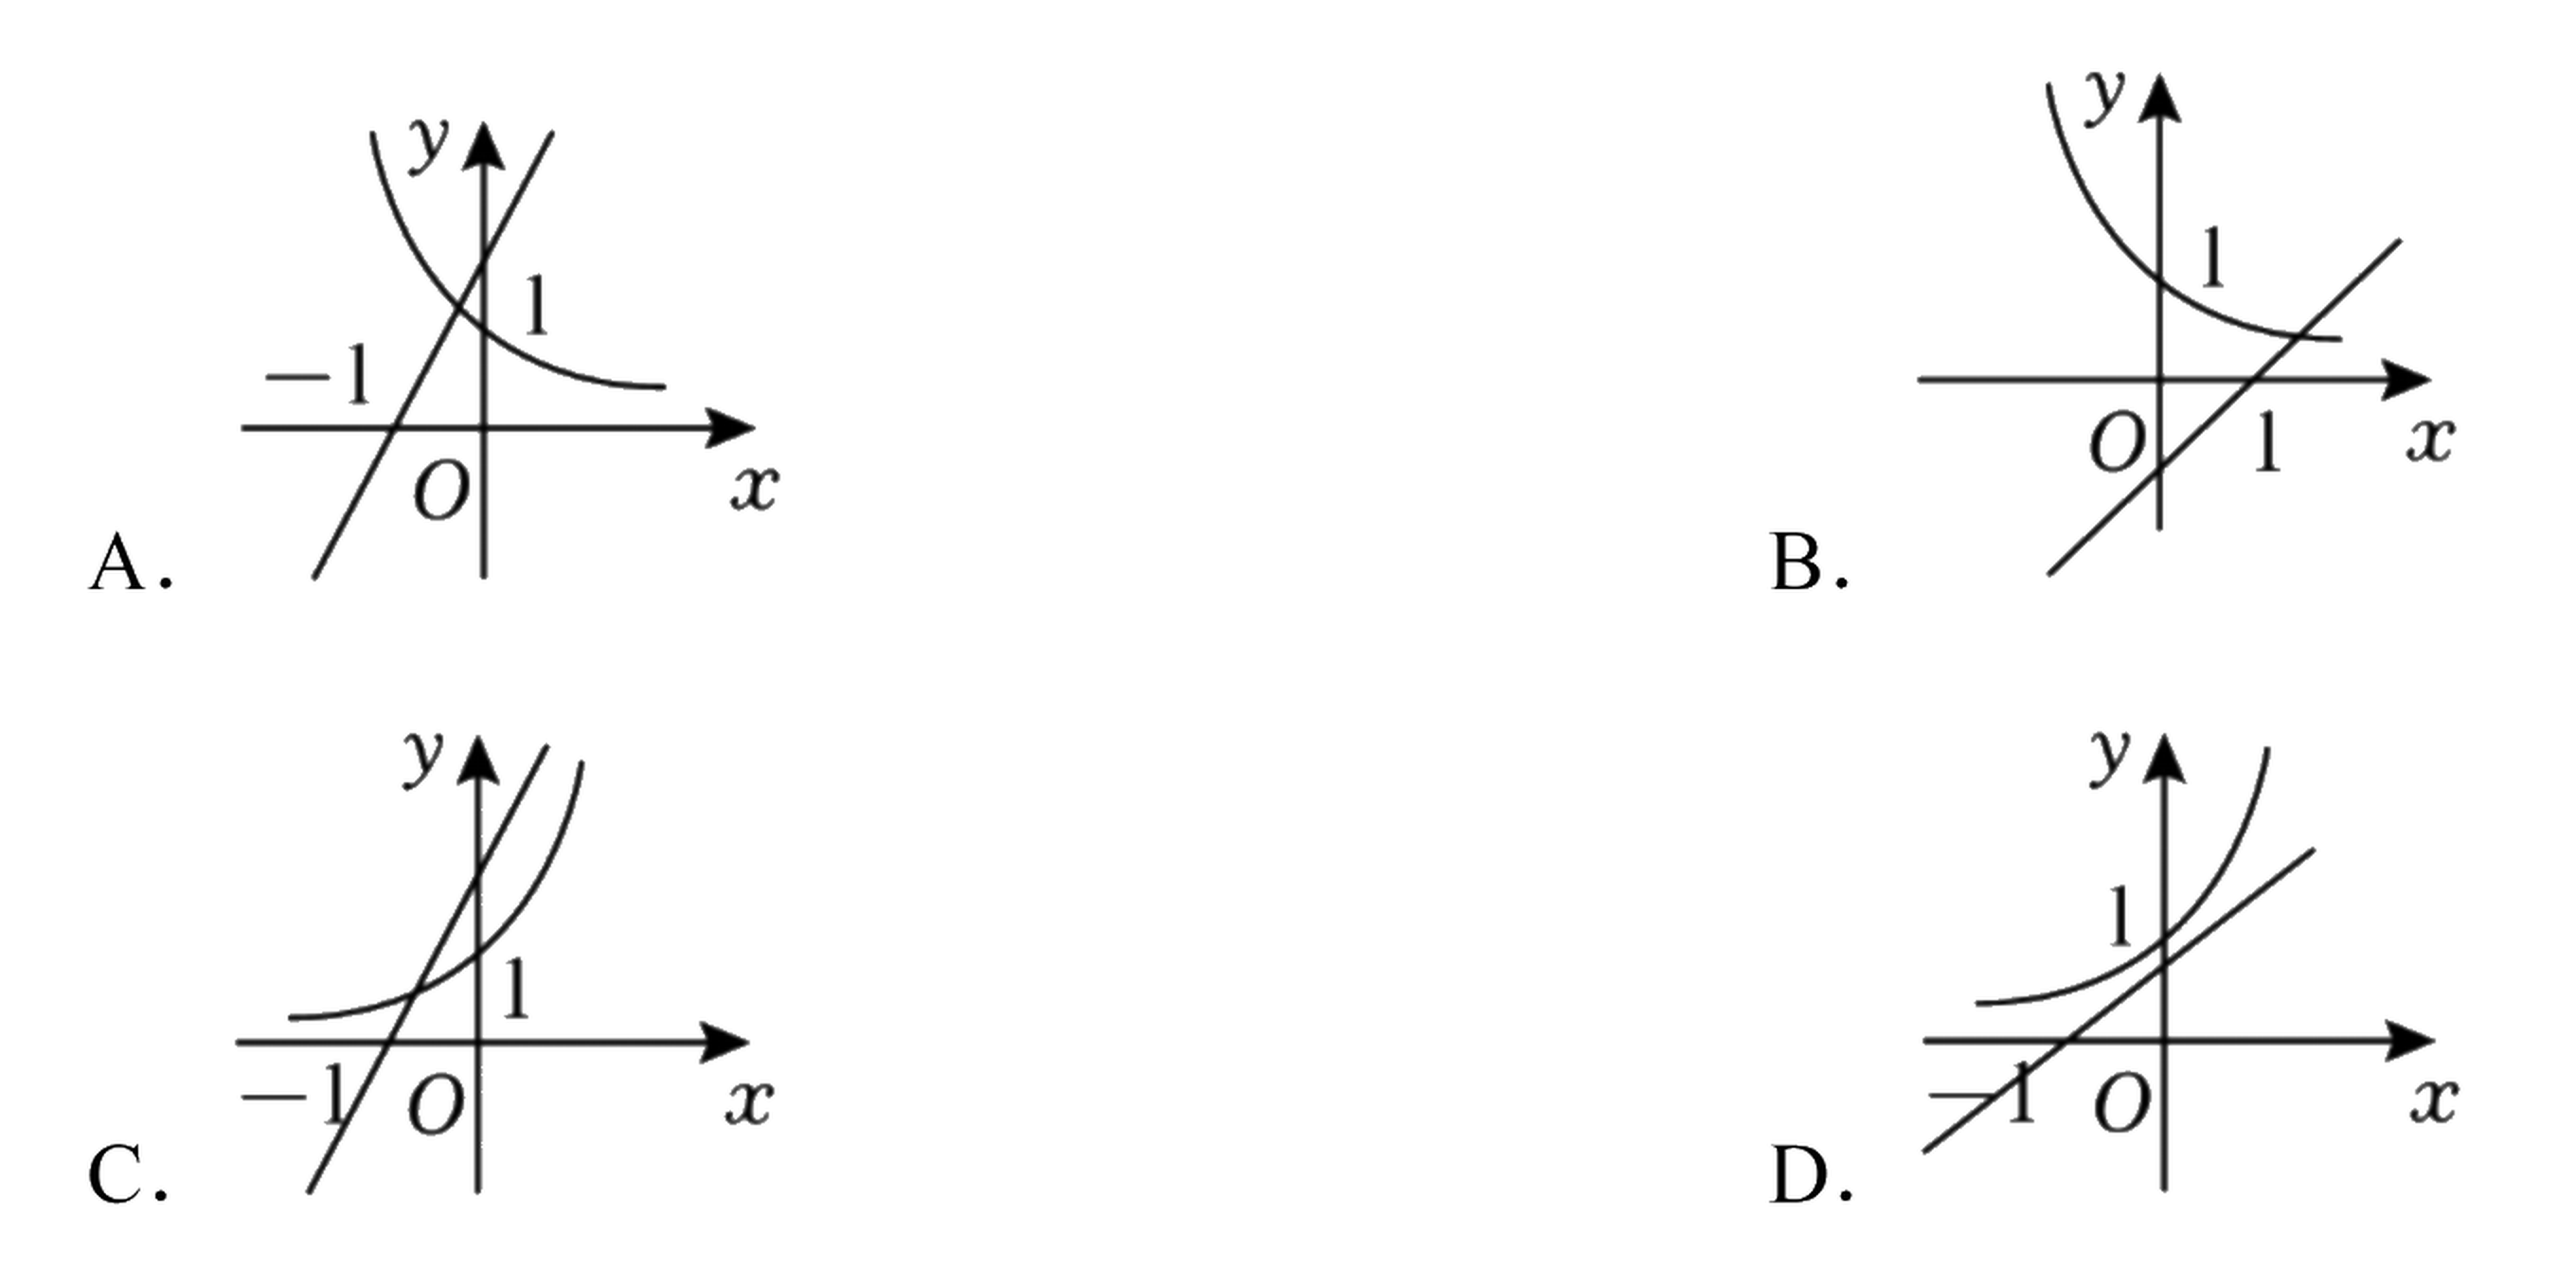
\includegraphics[width=0.80\textwidth]{figures/gao130_q15.png}
\end{center}

\ifanswer
\solbegin
\step{A 中，由指数函数 $y=a^x(a>0$ 且 $a\neq1)$ 图像递减得 $0<a<1$，}
\step{而一次函数 $y=a(x+1)$ 的图像与 $y$ 轴交点纵坐标为 $a>1$，二者矛盾，}
\step{所以 A 错；}
\step{由一次函数 $y=a(x+1)$ 的图像与 $x$ 轴交点横坐标为 $-1$，排除 B；}
\step{C 中，由指数函数 $y=a^x(a>0$ 且 $a\neq1)$ 图像递减得 $a>1$，}% 原卷"递减得 a>1"系笔误（应为"递增"），与 A 中"递减得 0<a<1"自相矛盾，照录
\step{而一次函数 $y=a(x+1)$ 的图像与 $y$ 轴交点纵坐标为 $a>1$，二者 $a$ 值吻合，}
\step{所以 C 对；}
\step{D 中，由一次函数 $y=a(x+1)$ 的图像得 $a=1$，与 $a>0$ 且 $a\neq1$ 矛盾，}
\step{所以 D 错.}
\step{故选 $C$.}
\solend
\fi

\item 设 $A_1$、$A_2$、$A_3$、$\cdots$、$A_7$ 是均含有 $2$ 个元素的集合，且 $A_1\cap A_7=\varnothing$，$A_i\cap A_{i+1}=\varnothing(i=1,2,3,\cdots,6)$，记 $B=A_1\cup A_2\cup A_3\cup\cdots\cup A_7$，则 $B$ 中元素个数的最小值是\mbox{（\quad）}

\keepwithprev
A. $4$\qquad B. $5$\qquad C. $6$\qquad D. $7$

\ifanswer
\solbegin
\step{取 $A_1=\{1,2\}$，$A_2=\{3,4\}$，$A_3=\{1,2\}$，$A_4=\{3,4\}$，$A_5=\{1,5\}$，$A_6=\{2,3\}$，$A_7=\{4,5\}$，}
\step{所以 $B$ 中元素个数的最小值是 $5$，故选 $B$.}
\solend
\fi

\end{enumerate}

\bigsec{三、解答题}

\begin{enumerate}
\setcounter{enumi}{16}

\item 已知全集为 $\R$，集合 $A=\{x\mid-2\leqslant x\leqslant5\}$，集合 $B=\{x\mid m-1\leqslant x\leqslant2m+1\}$．

(1) 求 $\overline{A}$；

(2) 若 $A\cup B=A$，求实数 $m$ 的取值范围．

\ifanswer
\solbegin
\step{(1) $(-\infty,-2)\cup(5,+\infty)$；}
\step{(2) 若 $A\cup B=A$，则 $B\subseteq A$，}
\step{当 $B=\varnothing$ 时，$m-1>2m+1$，解得 $m<-2$；}
\step{当 $B\neq\varnothing$ 时，$\begin{cases}m-1\leqslant2m+1\\m-1\geqslant-2\\2m+1\leqslant5\end{cases}$，解得 $-1\leqslant m\leqslant2$；}
\step{故实数 $m$ 的取值范围为 $\{m\mid-1\leqslant m\leqslant2$ 或 $m<-2\}$.}
\solend
\fi

\item 在不等式的应用中，有一些很基本而十分重要的不等式，如平均值不等式和三角不等式等，我们将其统称为基本不等式．

(1) 已知 $x$、$y$ 为正数，且 $2x+y=2$，求 $\dfrac1x+\dfrac2y$ 的最小值；

(2) 若关于 $x$ 的不等式 $\lvert x+1\rvert+\lvert2-x\rvert\geqslant a^2+a+1$ 对于一切实数 $x$ 都成立，求实数 $a$ 的取值范围．

\ifanswer
\solbegin
\step{(1) 因为 $x$、$y$ 为正数，且 $2x+y=2$，}
\step{所以 $\dfrac1x+\dfrac2y=\dfrac12\left(\dfrac1x+\dfrac2y\right)(2x+y)=\dfrac12\left(4+\dfrac yx+\dfrac{4x}y\right)\geqslant\dfrac12\left(4+2\sqrt{\dfrac yx\cdot\dfrac{4x}y}\right)=4$，}
\step{当且仅当 $\dfrac yx=\dfrac{4x}y$，即 $x=\dfrac12$，$y=1$ 时取等号，所以 $\dfrac1x+\dfrac2y$ 的最小值为 $4$；}
\step{(2) 由绝对值三角不等式得 $\lvert x+1\rvert+\lvert2-x\rvert\geqslant\lvert(x+1)+(2-x)\rvert=3$，}
\step{当且仅当 $-1\leqslant x\leqslant2$ 时取等号，所以 $\lvert x+1\rvert+\lvert2-x\rvert$ 的最小值为 $3$，}
\step{因为关于 $x$ 的不等式 $\lvert x+1\rvert+\lvert2-x\rvert\geqslant a^2+a+1$ 对于一切实数 $x$ 都成立，}
\step{所以 $a^2+a+1\leqslant3$，即 $a^2+a-2\leqslant0$，解得 $-2\leqslant a\leqslant1$，}
\step{所以实数 $a$ 的取值范围是 $[-2,1]$.}
\solend
\fi

\item 某医学专家为研究传染病传播中病毒细胞的发展规律，将病毒细胞注入一只小白鼠体内进行试验，经检测，病毒细胞的个数 $y$ 与天数 $x$ 的部分数据如表所示：

\begin{center}
\begin{tabular}{|c|c|c|c|c|c|c|c|}
\hline
天数 $(x)$ & $1$ & $2$ & $3$ & $4$ & $5$ & $6$ & $\cdots$ \\
\hline
病毒细胞的个数 $(y)$ & $1$ & $2$ & $4$ & $8$ & $16$ & $32$ & $\cdots$ \\
\hline
\end{tabular}
\end{center}

(1) 若病毒细胞的个数 $y$ 关于天数 $x$ 的变化规律可选用以下两个函数模型之一进行近似刻画：① $y=a\cdot b^x(a>0$，$b>0$，$b\neq1)$；② $y=a\cdot x^k(a\neq0)$．请结合表格中的数据，选择合适的函数模型，说明理由，并求出相应的函数表达式；

(2) 若该病毒细胞在小白鼠体内的个数超过 $10^8$，小白鼠将死亡，但注射某种药物，可杀死其体内 $98\%$ 的病毒细胞．则在 (1) 的条件下，为了使小白鼠在试验过程中不死亡，第一次最迟应在何时注射该种药物？（结果精确到天）

\ifanswer
\solbegin
\step{(1) 选择模型① $y=a\cdot b^x(a>0$，$b>0$，$b\neq1)$，理由如下：}
\step{观察表格数据，$y$ 的值随 $x$ 呈指数倍增：}
\step{$x=1$ 时，$y=1$，$x=2$ 时，$y=2$，$x=3$ 时，$y=4$，}
\step{后一天的病毒数是前一天的 $2$ 倍，符合指数增长的特征；}
\step{若选用幂函数模型 $y=a\cdot x^k$，代入前两组数据得 $a\cdot1^k=1$、$a\cdot2^k=2$，}
\step{解得 $a=1$，$k=1$，即 $y=x$，}
\step{但 $x=3$ 时，$y=3$ 与表格中 $y=4$ 严重不符，因此幂函数不匹配；}
\step{将 $(1,1)$ 代入 $y=a\cdot b^x$ 得 $a\cdot b=1$，}
\step{将 $(2,2)$ 代入得 $a\cdot b^2=2$，两式相除得 $b=2$，进而得 $a=\dfrac12$，}
\step{验证所有表格点均满足 $y=2^{x-1}$，最终函数表达式为 $y=2^{x-1}(x\in\N^*)$；}
\step{(2) 由题意得第一次注射药物前病毒细胞个数 $y$ 关于天数 $x(x\in\N^*)$ 的函数}
\step{关系式为 $y=2^{x-1}(x\in\N^*)$，}
\step{为了使小白鼠在试验过程中不死亡，则 $2^{x-1}\leqslant10^8$，}
\step{所以 $x-1\leqslant\log_210^8=8\log_210=\dfrac8{\lg2}$，解得 $x\leqslant1+\dfrac8{\lg2}\approx27.6$，}
\step{又 $x\in\N^*$，所以第一次最迟应在第 $27$ 天注射该种药物.}
\solend
\fi

\item 对在直角坐标系的第一象限内的任意两点 $(a,b)$，$(c,d)$ 作如下定义：$\dfrac ab>\dfrac cd$，那么称点 $(a,b)$ 是点 $(c,d)$ 的“上位点”，同时点 $(c,d)$ 是点 $(a,b)$ 的“下位点”．

(1) 试写出点 $(3,5)$ 的一个“上位点”坐标和一个“下位点”坐标；

(2) 设 $a$、$b$、$c$、$d$ 均为正数，且点 $(a,b)$ 是点 $(c,d)$ 的上位点，请判断点 $P(a+c,b+d)$ 是否既是点 $(a,b)$ 的“下位点”又是点 $(c,d)$ 的“上位点”，如果是，请证明；如果不是，请说明理由；

(3) 设正整数 $n$ 满足以下条件：对任意实数 $m\in\{t\mid0<t<4,t\in\Z\}$，总存在正整数 $k$，使得点 $(n,k)$ 既是点 $(4,m)$ 的“下位点”，又是点 $(5,m+1)$ 的“上位点”，求正整数 $n$ 的最小值．

\ifanswer
\solbegin
\step{(1) 由 $\dfrac34>\dfrac35>\dfrac36$ 得点 $(3,5)$ 的一个“上位点”的坐标为 $(3,4)$，}
\step{一个“下位点”的坐标为 $(3,6)$.}
\step{(2) 是，证明如下：}
\step{因为 $a$、$b$、$c$、$d$ 均为正数，点 $(a,b)$ 是点 $(c,d)$ 的“上位点”，}
\step{所以 $\dfrac ab>\dfrac cd$，所以 $ad>bc$，}
\step{因为 $\dfrac{a+c}{b+d}-\dfrac ab=\dfrac{b(a+c)-a(b+d)}{b(b+d)}=\dfrac{bc-ad}{b(b+d)}<0$，所以 $\dfrac{a+c}{b+d}<\dfrac ab$，}
\step{点 $P(a+c,b+d)$ 是点 $(a,b)$ 的“下位点”，}
\step{因为 $\dfrac{a+c}{b+d}-\dfrac cd=\dfrac{d(a+c)-c(b+d)}{d(b+d)}=\dfrac{ad-bc}{d(b+d)}>0$.}
\step{所以 $\dfrac{a+c}{b+d}>\dfrac cd$ 点 $P(a+c,b+d)$ 是点 $(c,d)$ 的“上位点”；}
\step{所以 $P(a+c,b+d)$ 既是点 $(a,b)$ 的“下位点”又是点 $(c,d)$ 的“上位点”；}
\step{(3) 由题意得 $m=1,2,3$，}
\step{由题意存在正整数 $k$：$\dfrac5{m+1}<\dfrac nk<\dfrac4m$，所以 $\begin{cases}\dfrac n4<k<\dfrac{2n}5(m=1)\\\dfrac n2<k<\dfrac{3n}5(m=2)\\\dfrac{3n}4<k<\dfrac{4n}5(m=3)\end{cases}$，}
\step{检验：$n=1,2,\cdots,8$ 不能同时找到整数 $k$，}
\step{$n=9$：$m=1$ 取 $k=3$，$m=2$ 取 $k=5$，$m=3$ 取 $k=7$，均满足，}
\step{所以正整数 $n$ 的最小值为 $9$.}
\solend
\fi

\end{enumerate}

\end{document}
"
% 紧凑版：xelatex "\def\iscompact{1}% 高一130_北郊高级中学_期中.tex
%   —— 高一上数学"2026-2027 年北郊高级中学高一上期中"（试卷版/答案版）
% 试卷版：xelatex 高一130_北郊高级中学_期中.tex
% 答案版：xelatex "\def\isanswer{1}% 高一130_北郊高级中学_期中.tex
%   —— 高一上数学"2026-2027 年北郊高级中学高一上期中"（试卷版/答案版）
% 试卷版：xelatex 高一130_北郊高级中学_期中.tex
% 答案版：xelatex "\def\isanswer{1}\input{高一130_北郊高级中学_期中.tex}"
% 紧凑版：xelatex "\def\iscompact{1}\input{高一130_北郊高级中学_期中.tex}"
%
% ① 原始材料：微信公众号"魔都数学加油站"文章，连载"27学年高一140"，原文标题
% "27学年高一140——2026-2027年上海市北郊高级中学高一上期中"；
% 原文链接：https://mp.weixin.qq.com/s/XBEYuTheiBoqu15dtLuD6A。
%   ★ 编号不一致说明：公众号连载号印"140"，与上一批已入库的"高一140 甘泉外国语"
%   （同一公众号另一篇文章、同为期中卷）撞号，系公众号笔误/重复。本仓库数字编号
%   02—143 中"高一130"一直空缺（连载 130 暂未见原文），故将本卷本地编号定为"高一130"、
%   填补该空缺，使数字编号连续（basename 全程为 高一130_北郊高级中学_期中）；
%   连载号 143 归正牌卷"上海中学 高一上期中"；本卷连载号仍印 140，见材料流转表。
%   卷面标题印"2026-2027 年北郊高级中学高一上期中"（卷面只有学校名、不含"上海市"、
%   不含任何期号/连载号），本稿照卷面录入；粉红色水印"魔都数学加油站"及页脚未录入。
% 正文为 9 张 PNG 页（01、04、05、06、09 为 2560x3620；02、03、07、08 为 4762x6735，
% 同一篇各页分辨率不同，逐页按各自分辨率放大核对），题目下印有【解析】，为讲评版。
% 题目、解析均据原图转录。
%
% 卷首标题：原卷印作"2026-2027 年北郊高级中学高一上期中"，年份区间按全稿惯例排
% en dash；原卷未印副标题，本卷为期中卷、跨集合与常用逻辑用语／不等式／函数三章，
% 按题目内容补出"集合与常用逻辑用语、不等式、函数"（与 125／126／128／129／131／132／133
% 同期中卷口径相同）。
%
% 题号体例：本卷共 18 题——一、填空题 3—12（10 题）、二、选择题 13—16（4 题）、
% 三、解答题 17—20（4 题）。三节分别 \setcounter{enumi}{2}／{12}／{16}。
% 原卷从第 3 题起、无第 1、2 题、**无第 21 题**（第 20 题解析续至 09 页，末行
% "所以正整数 n 的最小值为 9."，09 页下半页整片空白＋水印收尾、无第 10 页），本稿保留原题号。
%
% ② 与原卷的排版差异：
%   ① 原文从第 3 题起，本稿保留原题号；原卷止于第 20 题、无第 21 题、无附加题节；
%   ② 原卷每题下直接印【解析】，本稿按全稿惯例置于答案版；全卷 18 题均印【解析】、
%      无独立【答案】段，四道选择题答案在解析末句"故选 C／D／C／B"，括号
%      \mbox{（\quad）} 留空、不另提 \ans{}；全卷 0 处 \ans{}，答案版【解析】标记数 18＝题数；
%   ③ 原卷未印副标题，本稿按"知识模块"口径补出；
%   ④ 原卷填空横线按全稿惯例排为 \blankline[4.4em]；选择题括号排 \mbox{（\quad）}、
%      每个选项段前按惯例加 \keepwithprev；解答题不留作答区、不加 \anspace（讲评版）；
%   ⑤ 原卷数集排斜体 $R$／$N$，按全稿惯例改 \R／\N；空集记号 \varnothing；
%      绝对值排 \lvert…\rvert，集合描述竖线排 \mid；不等号按全稿惯例排 \leqslant／\geqslant；
%      补集照原卷上划线 \overline{A}；
%   ⑥ 1 幅插图 + 1 张印刷表格：第 15 题四幅坐标函数图象选项（04 页）取原卷截图
%      去粉色水印、去色、按原卷 2x2 排布合并为 figures/gao130_q15.png（非插图重绘），
%      放在 \keepwithprev 之后 \begin{center} 内、三版都出；第 19 题 (1) 印刷数据表格
%      （07 页，天数 x 1—6／病毒细胞个数 y 1/2/4/8/16/32）按原卷用 tabular 重排、
%      题干内三版都出（非插图）。
%      第 15 题是"二、选择题"节内带大图块的第三题（Q13 为节首题但无图），
%      在 \bigsec{二、选择题} 之前加 \needvspace{11cm} 连节标题一起量、Q15 \item 之前
%      加 \needvspace{9cm}——守卫必须放在 \bigsec 之前，放标题之后会让"二、选择题"
%      孤立在页末（B 类，照 高一26／40／59／136／140 成例）；三版切页审计均"合计异常：无"；
%   ⑦ 子题标号 (1)(2)(3) 原卷用半角括号，照录；圈数字 ①②③④ 照录；
%      数学式内半角逗号照录（如第 14 题 $(a>0,a\neq1)$、第 16 题
%      $(i=1,2,3,\cdots,6)$、第 20 题 $m=1,2,3$ 等）；
%      行末西文句点按全稿惯例照录；
%   ⑧ 题干中的中文弯引号按原卷照录（Q12"变项和"、Q20"上位点""下位点"等），
%      注释内一律 ASCII 引号；原卷"图像"用词逐处照录（Q9、Q15 均作"图像"）。
%
% ③ 行数复核：一条 \step = 原卷解析的一个印刷行（cases 块与 tabular 各作一个印刷行计）。
%   逐题 \step 条数，合计 98 条（Q3:3 Q4:2 Q5:2 Q6:1 Q7:1 Q8:3 Q9:5 Q10:10 Q11:6
%   Q12:7 Q13:1 Q14:2 Q15:10 Q16:2 Q17:5 Q18:8 Q19:15 Q20:15），与原卷印刷行逐题相等。
%
% ④ 判别式／子集符号结论：
%   判别式：全卷未出现判别式记号（无 $\Delta$、无 $\triangle$）；
%   子集符号：第 4 题题干"$B\subseteq A$"、第 4 题【解析】"$B\subseteq A$"、
%      第 17 题 (2)【解析】"$B\subseteq A$"三处原卷均印带下划线 $\subseteq$，逐处
%      放大核对、照录 \subseteq；全卷未出现单线 \subset。
%
% ⑤ 原卷存疑照录（均照录未改，正文对应处另有 % 注）：
%   ① 第 15 题【解析】"C 中，由指数函数 $y=a^x$ 图像递减得 $a>1$"——"递减"应为
%      "递增"之误（与同题 A 中"递减得 $0<a<1$"自相矛盾），原卷如此，照录并加注；
%   ② 第 16 题题干"$A_1\cap A_7=\varnothing$""$A_i\cap A_{i+1}=\varnothing$"
%      的空集记号与解析所列各集合逐处照录；
%   ③ 第 19 题 (2) 题干"可杀死其体内 98% 的病毒细胞"、解析 (2) 只按 $y=2^{x-1}$
%      与 $10^8$ 比较（未另计 98%），照录不补步。
%
% ⑥ 跨页续印按题合并：Q8 题干在 01 页末、解析在 02 页；Q9 题干在 02 页、
%   解析在 02 页；Q10 题干在 02 页、解析前 5 行在 02—03 页、后 5 行在 03 页；
%   Q12 题干跨 03 页、解析首 5 行在 03 页末、末行在 04 页；Q15 题干在 04 页、
%   四幅图与解析前段在 04 页、解析续在 05 页；Q17 解析跨 05—06 页；Q18 题干与
%   (1) 解析在 06 页、(2) 解析在 06—07 页；Q19 表格在 07 页、解析跨 07—08 页；
%   Q20 定义与三小问在 08 页、解析 (1)(2) 在 08—09 页、解析 (3) 在 09 页；
%   本稿按题连排，不丢行。
%
\documentclass[a4paper,11pt]{article}
\usepackage{common}

\begin{document}

\examtitlest[3]{2026--2027 年北郊高级中学高一上期中}{集合与常用逻辑用语、不等式、函数}

\bigsec{一、填空题}

\begin{enumerate}
\setcounter{enumi}{2}

\item 不等式 $\dfrac{x-3}{x+1}<2$ 的解集为\blankline[4.4em].

\ifanswer
\solbegin
\step{不等式 $\dfrac{x-3}{x+1}<2$ 可化为 $\dfrac{x-3}{x+1}-2<0$，即 $\dfrac{x-3-2(x+1)}{x+1}<0$，}
\step{化简为 $\dfrac{x+5}{x+1}>0$，解得 $x<-5$ 或 $x>-1$，}
\step{所以不等式的解集为 $\{x\mid x<-5$ 或 $x>-1\}$.}
\solend
\fi

\item 已知集合 $A=\{x\mid0<x<a\}$，$B=\{x\mid1<x<2\}$，若 $B\subseteq A$，则实数 $a$ 的取值范围为\blankline[4.4em].

\ifanswer
\solbegin
\step{已知集合 $A=\{x\mid0<x<a\}$，$B=\{x\mid1<x<2\}$，}
\step{若 $B\subseteq A$，则 $a\geqslant2$，所以实数 $a$ 的取值范围是 $\{a\mid a\geqslant2\}$.}
\solend
\fi

\item 已知关于 $x$ 的方程 $x^2+x+c=0$ 的两个实数根为 $x_1$、$x_2$，若 $x_1^2x_2+x_2^2x_1=3$，则实数 $c=$\blankline[4.4em].

\ifanswer
\solbegin
\step{由韦达定理得 $x_1+x_2=-1$，$x_1x_2=c$，所以 $x_1^2x_2+x_2^2x_1=(x_1+x_2)x_1x_2=-c=3$，}
\step{所以 $c=-3$.}
\solend
\fi

\item 已知 $10^x=3$，$10^y=64$，则 $10^{x-\frac y3}=$\blankline[4.4em].

\ifanswer
\solbegin
\step{$10^{x-\frac y3}=10^x\div\sqrt[3]{10^y}=\dfrac34$.}
\solend
\fi

\item 若 $\lg2=a$，则可用 $a$ 表示 $\log_280=$\blankline[4.4em].

\ifanswer
\solbegin
\step{$\log_280=\dfrac{\lg80}{\lg2}=\dfrac{\lg10+\lg8}{\lg2}=\dfrac{1+3\lg2}{\lg2}=\dfrac{1+3a}{a}$.}
\solend
\fi

\item 已知 $a+2b=1$，则 $3^a+9^b$ 的最小值为\blankline[4.4em].

\ifanswer
\solbegin
\step{因为 $a+2b=1$，所以 $3^a+9^b=3^a+3^{2b}\geqslant2\sqrt{3^a\cdot3^{2b}}=2\sqrt{3^{a+2b}}=2\sqrt3$，}
\step{当且仅当 $3^a=3^{2b}$，且 $a+2b=1$，即 $a=\dfrac12$，$b=\dfrac14$ 时取等号，}
\step{故最小值为 $2\sqrt3$.}
\solend
\fi

\item 下列函数的图像关于原点成中心对称，且在区间 $(0,+\infty)$ 上是严格增函数的是\blankline[4.4em]（请填写全部正确的序号）.

① $y=\sqrt{x}$；② $y=\sqrt[3]{x}$；③ $y=x^{\frac23}$；④ $y=x^{-\frac13}$.

\ifanswer
\solbegin
\step{① $y=\sqrt{x}$ 的定义域为 $[0,+\infty)$，故其图像不关于原点成中心对称，①错误；}
\step{② $y=\sqrt[3]{x}$ 是奇函数，且在区间 $(0,+\infty)$ 上是严格增函数，②正确；}
\step{③ $y=x^{\frac23}$ 是偶函数，其图像关于 $y$ 轴对称，不关于原点成中心对称，③错误；}
\step{④由于幂指数 $-\dfrac13<0$，故 $y=x^{-\frac13}$ 在区间 $(0,+\infty)$ 上是严格减函数，④错误.}
\step{故正确的是②.}
\solend
\fi

\item 设 $a>0$ 且 $a\neq1$，若函数 $y=a^{2x}+2a^x-3$ 在区间 $[-1,1]$ 上的最大值为 $21$，则实数 $a$ 的值为\blankline[4.4em].

\ifanswer
\solbegin
\step{令 $t=a^x$，$x\in[-1,1]$，}
\step{当 $a>1$ 时，$t=a^x$ 严格增，则 $t\in\left[\dfrac1a,a\right]$，}
\step{则函数 $y=t^2+2t-3$，对称轴为 $t=-1$，}
\step{所以函数 $y=t^2+2t-3$ 在 $\left[\dfrac1a,a\right]$ 上严格增，}
\step{所以当 $t=a$ 时，$y$ 取得最大值 $a^2+2a-3=21$，解得 $a=4$ 或 $-6$（舍去）；}
\step{当 $0<a<1$ 时，$t=a^x$ 严格减，则 $t\in\left[a,\dfrac1a\right]$，}
\step{则函数 $y=t^2+2t-3$，对称轴为 $t=-1$，}
\step{所以函数 $y=t^2+2t-3$ 在 $\left[a,\dfrac1a\right]$ 上严格增，}
\step{所以当 $t=\dfrac1a$ 时，$y$ 取得最大值 $\dfrac1{a^2}+\dfrac2a-3=21$，解得 $a=\dfrac14$ 或 $-\dfrac16$（舍去）；}
\step{综上所述，实数 $a$ 的值为 $4$ 或 $\dfrac14$.}
\solend
\fi

\item 在关于 $x$ 的不等式 $x^2+(m+1)x+m<0$ 的解集中恰有两个整数，则实数 $m$ 的取值范围是\blankline[4.4em].

\ifanswer
\solbegin
\step{关于 $x$ 的不等式 $x^2+(m+1)x+m<0$ 可化为 $(x+1)(x+m)<0$，}
\step{当 $m>1$ 时，$-m<-1$，解不等式得 $-m<x<-1$；}
\step{当 $m<1$ 时，$-m>-1$，解不等式得 $-1<x<-m$；}
\step{由不等式的解集中恰有两个整数，}
\step{则 $-4\leqslant-m<-3$ 或 $1<-m\leqslant2$，即 $3<m\leqslant4$ 或 $-2\leqslant m<-1$，}
\step{所以 $m$ 的取值范围是 $[-2,-1)\cup(3,4]$.}
\solend
\fi

\item 已知集合 $M$ 的元素均为正整数，定义集合 $M$ 的“变项和”为：将 $M$ 中每个元素 $m$ 都乘以 $(-1)^m$ 后再求和．若集合 $A=\{n\mid1\leqslant n\leqslant20,n\in\N\}$，则集合 $A$ 的所有非空子集的“变项和”的总和为\blankline[4.4em].

\ifanswer
\solbegin
\step{集合 $A=\{n\mid1\leqslant n\leqslant20,n\in\N\}$ 中一共有 $20$ 个元素，}
\step{固定选中 $k$，剩下 $19$ 个元素任选，共 $2^{19}$ 个子集包含 $k$，每个 $k$ 贡献 $(-1)^k\cdot k\cdot2^{19}$，}
\step{$A=\{1,2,\cdots,20\}$，}
\step{奇数 $k=1,3,\cdots,19$，共 $10$ 个，$(-1)^k\cdot k=-k$，}
\step{偶数 $k=2,4,\cdots,20$，共 $10$ 个，$(-1)^k\cdot k=k$，}
\step{所以集合 $A$ 的所有非空子集的“变项和”的总和}
\step{为 $S=2^{19}\times[(-1+2)+(-3+4)+\cdots+(-19+20)]=2^{19}\times10=524880$.}
\solend
\fi

\end{enumerate}

% 第 15 题四幅图是"二、选择题"节内大图块；守卫须放在 \bigsec 之前连节标题一起量，
% 否则"二、选择题"会孤立在页末（B 类，照 高一26／40／59／136／140 成例）
\needvspace{11cm}
\bigsec{二、选择题}

\begin{enumerate}
\setcounter{enumi}{12}

\item 设 $ab>0$，则“$a>b$”是“$\dfrac1a<\dfrac1b$”的\mbox{（\quad）}

\keepwithprev
A. 充分非必要条件\qquad B. 必要非充分条件

C. 充要条件\qquad D. 既非充分也非必要条件

\ifanswer
\solbegin
\step{因为 $ab>0$，所以 $a>b\Leftrightarrow\dfrac1a<\dfrac1b$，故选 $C$.}
\solend
\fi

\item 已知 $A=\log_ax$，$B=\log_ay(a>0,a\neq1)$，则 $\log_a\dfrac{x^2}{\sqrt y}=$\mbox{（\quad）}

\keepwithprev
A. $\dfrac{A^2}{\sqrt B}$\qquad B. $2A^2B$\qquad C. $4AB$\qquad D. $2A-\dfrac12B$

\ifanswer
\solbegin
\step{由已知得 $x=a^A$，$y=a^B$，}
\step{所以 $\log_a\dfrac{x^2}{\sqrt y}=\log_a\dfrac{(a^A)^2}{\sqrt{a^B}}=\log_a\dfrac{a^{2A}}{a^{\frac12B}}=\log_a a^{2A-\frac12B}=2A-\dfrac12B$. 故选 $D$.}
\solend
\fi

% 第 15 题四幅坐标函数图象选项是一整块，守卫放在 \item 之前
\needvspace{9cm}
\item 在同一平面直角坐标系中，指数函数 $y=a^x(a>0$ 且 $a\neq1)$ 和一次函数 $y=a(x+1)$ 的图像关系可能是\mbox{（\quad）}

\keepwithprev
\begin{center}
% 四幅坐标函数图象选项取原卷 04 页截图去粉色水印、去色，按原卷 2x2 排布合并为一张
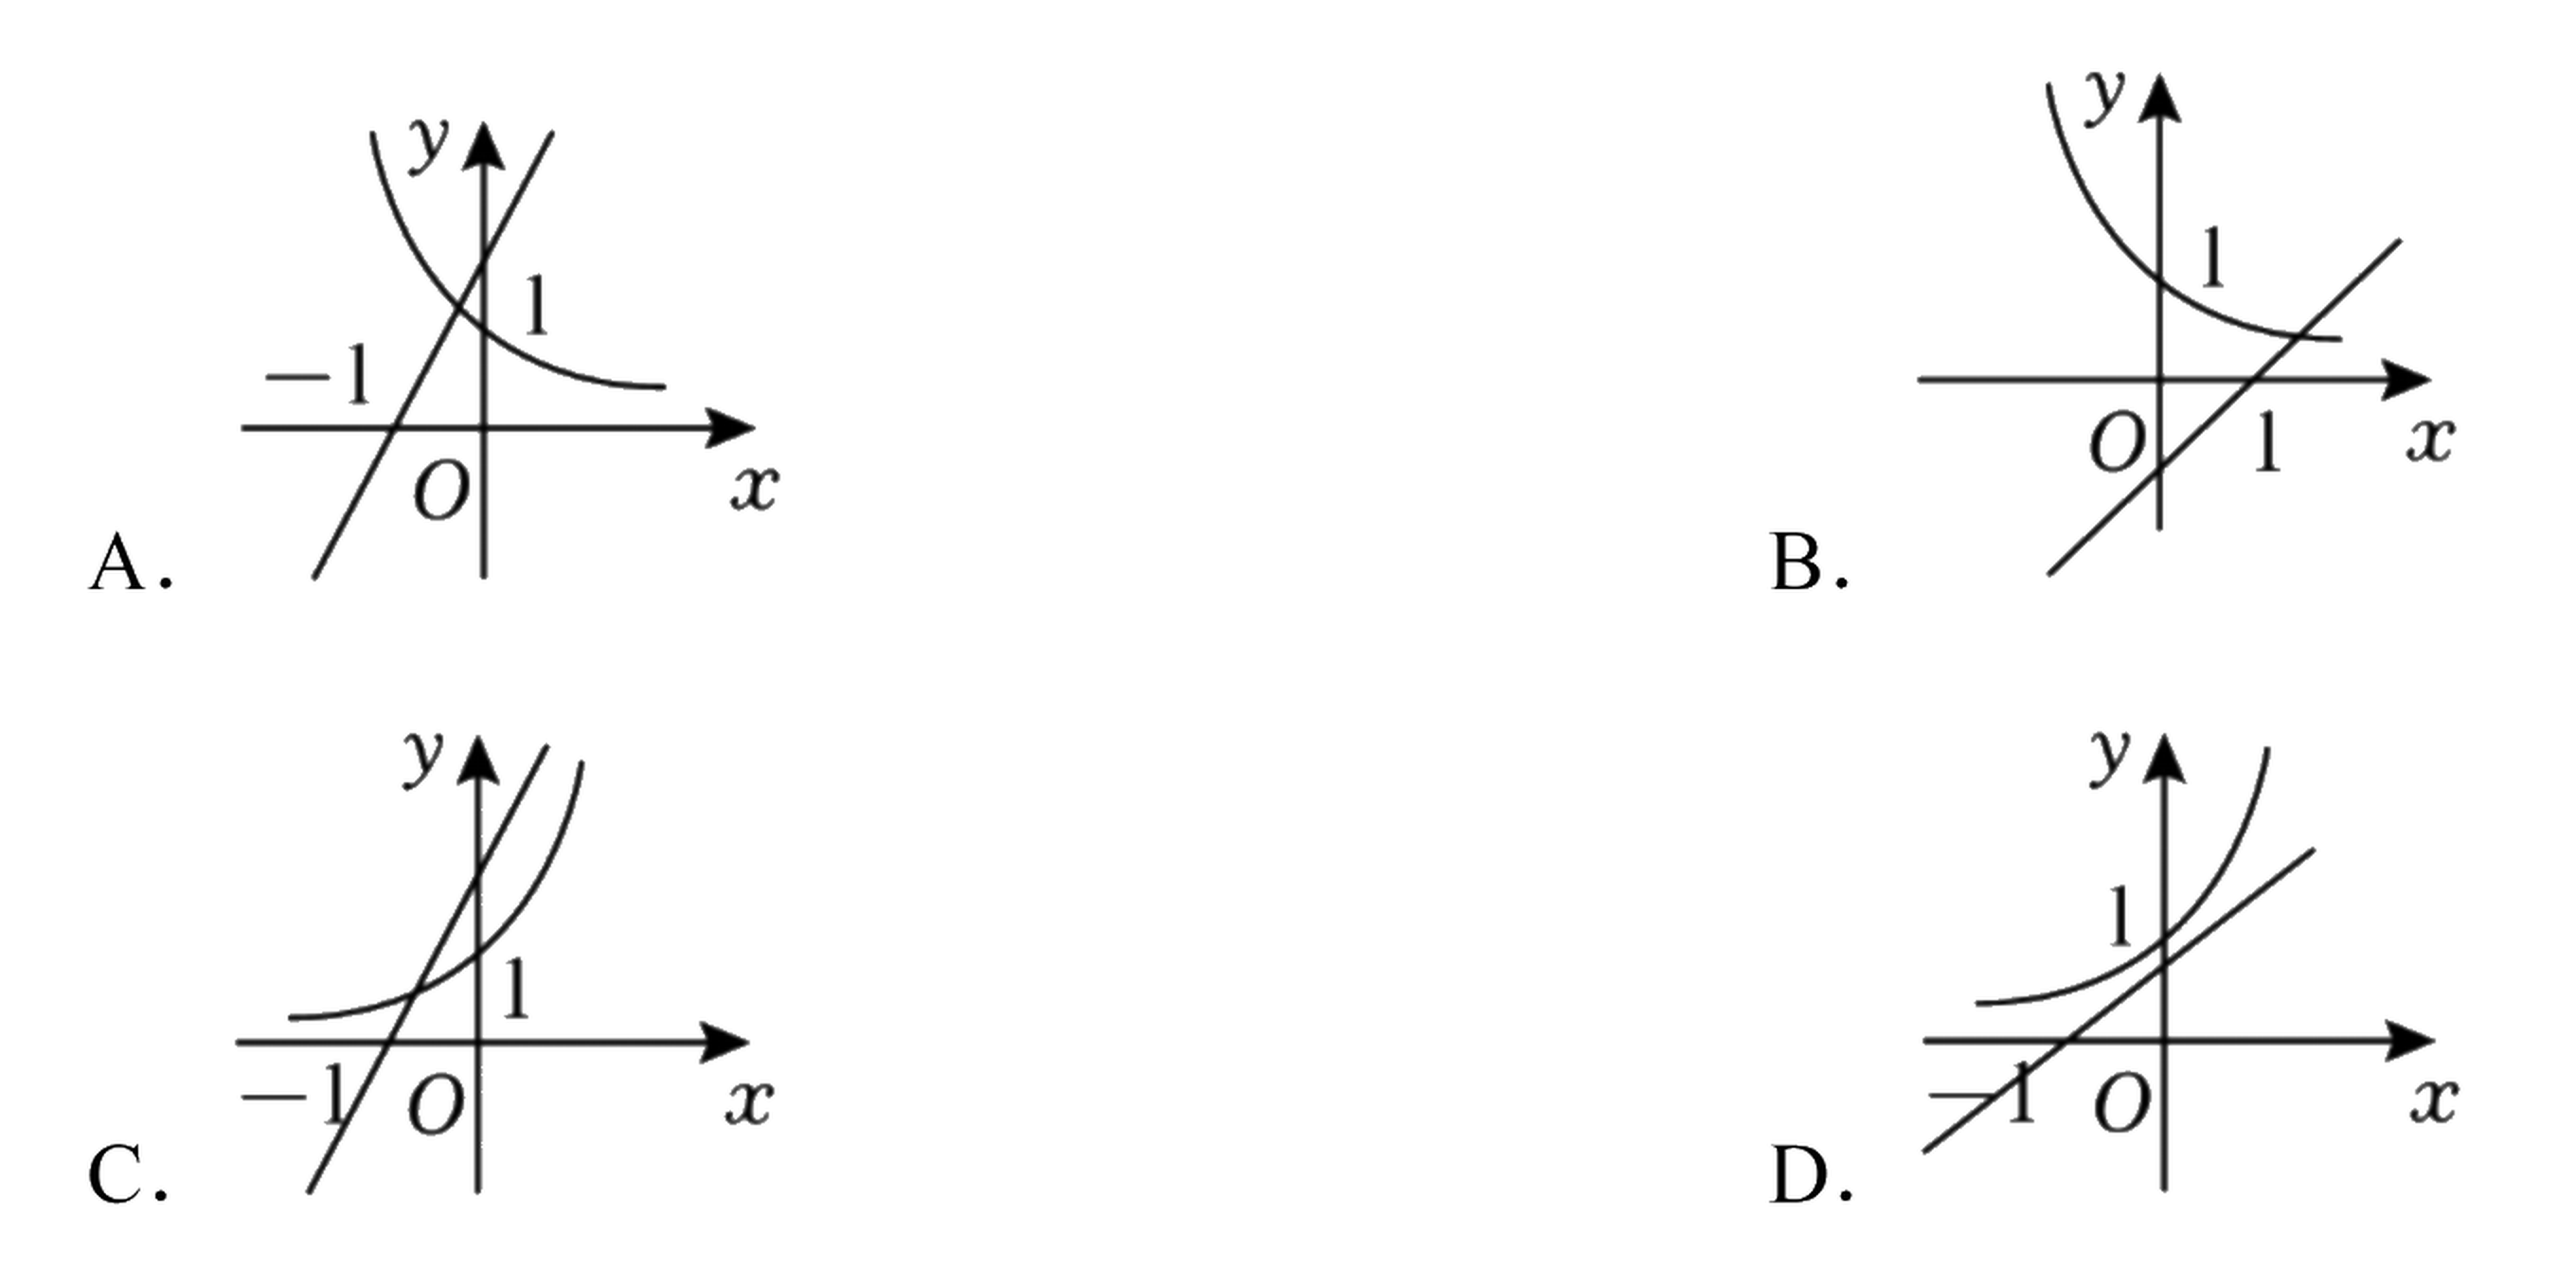
\includegraphics[width=0.80\textwidth]{figures/gao130_q15.png}
\end{center}

\ifanswer
\solbegin
\step{A 中，由指数函数 $y=a^x(a>0$ 且 $a\neq1)$ 图像递减得 $0<a<1$，}
\step{而一次函数 $y=a(x+1)$ 的图像与 $y$ 轴交点纵坐标为 $a>1$，二者矛盾，}
\step{所以 A 错；}
\step{由一次函数 $y=a(x+1)$ 的图像与 $x$ 轴交点横坐标为 $-1$，排除 B；}
\step{C 中，由指数函数 $y=a^x(a>0$ 且 $a\neq1)$ 图像递减得 $a>1$，}% 原卷"递减得 a>1"系笔误（应为"递增"），与 A 中"递减得 0<a<1"自相矛盾，照录
\step{而一次函数 $y=a(x+1)$ 的图像与 $y$ 轴交点纵坐标为 $a>1$，二者 $a$ 值吻合，}
\step{所以 C 对；}
\step{D 中，由一次函数 $y=a(x+1)$ 的图像得 $a=1$，与 $a>0$ 且 $a\neq1$ 矛盾，}
\step{所以 D 错.}
\step{故选 $C$.}
\solend
\fi

\item 设 $A_1$、$A_2$、$A_3$、$\cdots$、$A_7$ 是均含有 $2$ 个元素的集合，且 $A_1\cap A_7=\varnothing$，$A_i\cap A_{i+1}=\varnothing(i=1,2,3,\cdots,6)$，记 $B=A_1\cup A_2\cup A_3\cup\cdots\cup A_7$，则 $B$ 中元素个数的最小值是\mbox{（\quad）}

\keepwithprev
A. $4$\qquad B. $5$\qquad C. $6$\qquad D. $7$

\ifanswer
\solbegin
\step{取 $A_1=\{1,2\}$，$A_2=\{3,4\}$，$A_3=\{1,2\}$，$A_4=\{3,4\}$，$A_5=\{1,5\}$，$A_6=\{2,3\}$，$A_7=\{4,5\}$，}
\step{所以 $B$ 中元素个数的最小值是 $5$，故选 $B$.}
\solend
\fi

\end{enumerate}

\bigsec{三、解答题}

\begin{enumerate}
\setcounter{enumi}{16}

\item 已知全集为 $\R$，集合 $A=\{x\mid-2\leqslant x\leqslant5\}$，集合 $B=\{x\mid m-1\leqslant x\leqslant2m+1\}$．

(1) 求 $\overline{A}$；

(2) 若 $A\cup B=A$，求实数 $m$ 的取值范围．

\ifanswer
\solbegin
\step{(1) $(-\infty,-2)\cup(5,+\infty)$；}
\step{(2) 若 $A\cup B=A$，则 $B\subseteq A$，}
\step{当 $B=\varnothing$ 时，$m-1>2m+1$，解得 $m<-2$；}
\step{当 $B\neq\varnothing$ 时，$\begin{cases}m-1\leqslant2m+1\\m-1\geqslant-2\\2m+1\leqslant5\end{cases}$，解得 $-1\leqslant m\leqslant2$；}
\step{故实数 $m$ 的取值范围为 $\{m\mid-1\leqslant m\leqslant2$ 或 $m<-2\}$.}
\solend
\fi

\item 在不等式的应用中，有一些很基本而十分重要的不等式，如平均值不等式和三角不等式等，我们将其统称为基本不等式．

(1) 已知 $x$、$y$ 为正数，且 $2x+y=2$，求 $\dfrac1x+\dfrac2y$ 的最小值；

(2) 若关于 $x$ 的不等式 $\lvert x+1\rvert+\lvert2-x\rvert\geqslant a^2+a+1$ 对于一切实数 $x$ 都成立，求实数 $a$ 的取值范围．

\ifanswer
\solbegin
\step{(1) 因为 $x$、$y$ 为正数，且 $2x+y=2$，}
\step{所以 $\dfrac1x+\dfrac2y=\dfrac12\left(\dfrac1x+\dfrac2y\right)(2x+y)=\dfrac12\left(4+\dfrac yx+\dfrac{4x}y\right)\geqslant\dfrac12\left(4+2\sqrt{\dfrac yx\cdot\dfrac{4x}y}\right)=4$，}
\step{当且仅当 $\dfrac yx=\dfrac{4x}y$，即 $x=\dfrac12$，$y=1$ 时取等号，所以 $\dfrac1x+\dfrac2y$ 的最小值为 $4$；}
\step{(2) 由绝对值三角不等式得 $\lvert x+1\rvert+\lvert2-x\rvert\geqslant\lvert(x+1)+(2-x)\rvert=3$，}
\step{当且仅当 $-1\leqslant x\leqslant2$ 时取等号，所以 $\lvert x+1\rvert+\lvert2-x\rvert$ 的最小值为 $3$，}
\step{因为关于 $x$ 的不等式 $\lvert x+1\rvert+\lvert2-x\rvert\geqslant a^2+a+1$ 对于一切实数 $x$ 都成立，}
\step{所以 $a^2+a+1\leqslant3$，即 $a^2+a-2\leqslant0$，解得 $-2\leqslant a\leqslant1$，}
\step{所以实数 $a$ 的取值范围是 $[-2,1]$.}
\solend
\fi

\item 某医学专家为研究传染病传播中病毒细胞的发展规律，将病毒细胞注入一只小白鼠体内进行试验，经检测，病毒细胞的个数 $y$ 与天数 $x$ 的部分数据如表所示：

\begin{center}
\begin{tabular}{|c|c|c|c|c|c|c|c|}
\hline
天数 $(x)$ & $1$ & $2$ & $3$ & $4$ & $5$ & $6$ & $\cdots$ \\
\hline
病毒细胞的个数 $(y)$ & $1$ & $2$ & $4$ & $8$ & $16$ & $32$ & $\cdots$ \\
\hline
\end{tabular}
\end{center}

(1) 若病毒细胞的个数 $y$ 关于天数 $x$ 的变化规律可选用以下两个函数模型之一进行近似刻画：① $y=a\cdot b^x(a>0$，$b>0$，$b\neq1)$；② $y=a\cdot x^k(a\neq0)$．请结合表格中的数据，选择合适的函数模型，说明理由，并求出相应的函数表达式；

(2) 若该病毒细胞在小白鼠体内的个数超过 $10^8$，小白鼠将死亡，但注射某种药物，可杀死其体内 $98\%$ 的病毒细胞．则在 (1) 的条件下，为了使小白鼠在试验过程中不死亡，第一次最迟应在何时注射该种药物？（结果精确到天）

\ifanswer
\solbegin
\step{(1) 选择模型① $y=a\cdot b^x(a>0$，$b>0$，$b\neq1)$，理由如下：}
\step{观察表格数据，$y$ 的值随 $x$ 呈指数倍增：}
\step{$x=1$ 时，$y=1$，$x=2$ 时，$y=2$，$x=3$ 时，$y=4$，}
\step{后一天的病毒数是前一天的 $2$ 倍，符合指数增长的特征；}
\step{若选用幂函数模型 $y=a\cdot x^k$，代入前两组数据得 $a\cdot1^k=1$、$a\cdot2^k=2$，}
\step{解得 $a=1$，$k=1$，即 $y=x$，}
\step{但 $x=3$ 时，$y=3$ 与表格中 $y=4$ 严重不符，因此幂函数不匹配；}
\step{将 $(1,1)$ 代入 $y=a\cdot b^x$ 得 $a\cdot b=1$，}
\step{将 $(2,2)$ 代入得 $a\cdot b^2=2$，两式相除得 $b=2$，进而得 $a=\dfrac12$，}
\step{验证所有表格点均满足 $y=2^{x-1}$，最终函数表达式为 $y=2^{x-1}(x\in\N^*)$；}
\step{(2) 由题意得第一次注射药物前病毒细胞个数 $y$ 关于天数 $x(x\in\N^*)$ 的函数}
\step{关系式为 $y=2^{x-1}(x\in\N^*)$，}
\step{为了使小白鼠在试验过程中不死亡，则 $2^{x-1}\leqslant10^8$，}
\step{所以 $x-1\leqslant\log_210^8=8\log_210=\dfrac8{\lg2}$，解得 $x\leqslant1+\dfrac8{\lg2}\approx27.6$，}
\step{又 $x\in\N^*$，所以第一次最迟应在第 $27$ 天注射该种药物.}
\solend
\fi

\item 对在直角坐标系的第一象限内的任意两点 $(a,b)$，$(c,d)$ 作如下定义：$\dfrac ab>\dfrac cd$，那么称点 $(a,b)$ 是点 $(c,d)$ 的“上位点”，同时点 $(c,d)$ 是点 $(a,b)$ 的“下位点”．

(1) 试写出点 $(3,5)$ 的一个“上位点”坐标和一个“下位点”坐标；

(2) 设 $a$、$b$、$c$、$d$ 均为正数，且点 $(a,b)$ 是点 $(c,d)$ 的上位点，请判断点 $P(a+c,b+d)$ 是否既是点 $(a,b)$ 的“下位点”又是点 $(c,d)$ 的“上位点”，如果是，请证明；如果不是，请说明理由；

(3) 设正整数 $n$ 满足以下条件：对任意实数 $m\in\{t\mid0<t<4,t\in\Z\}$，总存在正整数 $k$，使得点 $(n,k)$ 既是点 $(4,m)$ 的“下位点”，又是点 $(5,m+1)$ 的“上位点”，求正整数 $n$ 的最小值．

\ifanswer
\solbegin
\step{(1) 由 $\dfrac34>\dfrac35>\dfrac36$ 得点 $(3,5)$ 的一个“上位点”的坐标为 $(3,4)$，}
\step{一个“下位点”的坐标为 $(3,6)$.}
\step{(2) 是，证明如下：}
\step{因为 $a$、$b$、$c$、$d$ 均为正数，点 $(a,b)$ 是点 $(c,d)$ 的“上位点”，}
\step{所以 $\dfrac ab>\dfrac cd$，所以 $ad>bc$，}
\step{因为 $\dfrac{a+c}{b+d}-\dfrac ab=\dfrac{b(a+c)-a(b+d)}{b(b+d)}=\dfrac{bc-ad}{b(b+d)}<0$，所以 $\dfrac{a+c}{b+d}<\dfrac ab$，}
\step{点 $P(a+c,b+d)$ 是点 $(a,b)$ 的“下位点”，}
\step{因为 $\dfrac{a+c}{b+d}-\dfrac cd=\dfrac{d(a+c)-c(b+d)}{d(b+d)}=\dfrac{ad-bc}{d(b+d)}>0$.}
\step{所以 $\dfrac{a+c}{b+d}>\dfrac cd$ 点 $P(a+c,b+d)$ 是点 $(c,d)$ 的“上位点”；}
\step{所以 $P(a+c,b+d)$ 既是点 $(a,b)$ 的“下位点”又是点 $(c,d)$ 的“上位点”；}
\step{(3) 由题意得 $m=1,2,3$，}
\step{由题意存在正整数 $k$：$\dfrac5{m+1}<\dfrac nk<\dfrac4m$，所以 $\begin{cases}\dfrac n4<k<\dfrac{2n}5(m=1)\\\dfrac n2<k<\dfrac{3n}5(m=2)\\\dfrac{3n}4<k<\dfrac{4n}5(m=3)\end{cases}$，}
\step{检验：$n=1,2,\cdots,8$ 不能同时找到整数 $k$，}
\step{$n=9$：$m=1$ 取 $k=3$，$m=2$ 取 $k=5$，$m=3$ 取 $k=7$，均满足，}
\step{所以正整数 $n$ 的最小值为 $9$.}
\solend
\fi

\end{enumerate}

\end{document}
"
% 紧凑版：xelatex "\def\iscompact{1}% 高一130_北郊高级中学_期中.tex
%   —— 高一上数学"2026-2027 年北郊高级中学高一上期中"（试卷版/答案版）
% 试卷版：xelatex 高一130_北郊高级中学_期中.tex
% 答案版：xelatex "\def\isanswer{1}\input{高一130_北郊高级中学_期中.tex}"
% 紧凑版：xelatex "\def\iscompact{1}\input{高一130_北郊高级中学_期中.tex}"
%
% ① 原始材料：微信公众号"魔都数学加油站"文章，连载"27学年高一140"，原文标题
% "27学年高一140——2026-2027年上海市北郊高级中学高一上期中"；
% 原文链接：https://mp.weixin.qq.com/s/XBEYuTheiBoqu15dtLuD6A。
%   ★ 编号不一致说明：公众号连载号印"140"，与上一批已入库的"高一140 甘泉外国语"
%   （同一公众号另一篇文章、同为期中卷）撞号，系公众号笔误/重复。本仓库数字编号
%   02—143 中"高一130"一直空缺（连载 130 暂未见原文），故将本卷本地编号定为"高一130"、
%   填补该空缺，使数字编号连续（basename 全程为 高一130_北郊高级中学_期中）；
%   连载号 143 归正牌卷"上海中学 高一上期中"；本卷连载号仍印 140，见材料流转表。
%   卷面标题印"2026-2027 年北郊高级中学高一上期中"（卷面只有学校名、不含"上海市"、
%   不含任何期号/连载号），本稿照卷面录入；粉红色水印"魔都数学加油站"及页脚未录入。
% 正文为 9 张 PNG 页（01、04、05、06、09 为 2560x3620；02、03、07、08 为 4762x6735，
% 同一篇各页分辨率不同，逐页按各自分辨率放大核对），题目下印有【解析】，为讲评版。
% 题目、解析均据原图转录。
%
% 卷首标题：原卷印作"2026-2027 年北郊高级中学高一上期中"，年份区间按全稿惯例排
% en dash；原卷未印副标题，本卷为期中卷、跨集合与常用逻辑用语／不等式／函数三章，
% 按题目内容补出"集合与常用逻辑用语、不等式、函数"（与 125／126／128／129／131／132／133
% 同期中卷口径相同）。
%
% 题号体例：本卷共 18 题——一、填空题 3—12（10 题）、二、选择题 13—16（4 题）、
% 三、解答题 17—20（4 题）。三节分别 \setcounter{enumi}{2}／{12}／{16}。
% 原卷从第 3 题起、无第 1、2 题、**无第 21 题**（第 20 题解析续至 09 页，末行
% "所以正整数 n 的最小值为 9."，09 页下半页整片空白＋水印收尾、无第 10 页），本稿保留原题号。
%
% ② 与原卷的排版差异：
%   ① 原文从第 3 题起，本稿保留原题号；原卷止于第 20 题、无第 21 题、无附加题节；
%   ② 原卷每题下直接印【解析】，本稿按全稿惯例置于答案版；全卷 18 题均印【解析】、
%      无独立【答案】段，四道选择题答案在解析末句"故选 C／D／C／B"，括号
%      \mbox{（\quad）} 留空、不另提 \ans{}；全卷 0 处 \ans{}，答案版【解析】标记数 18＝题数；
%   ③ 原卷未印副标题，本稿按"知识模块"口径补出；
%   ④ 原卷填空横线按全稿惯例排为 \blankline[4.4em]；选择题括号排 \mbox{（\quad）}、
%      每个选项段前按惯例加 \keepwithprev；解答题不留作答区、不加 \anspace（讲评版）；
%   ⑤ 原卷数集排斜体 $R$／$N$，按全稿惯例改 \R／\N；空集记号 \varnothing；
%      绝对值排 \lvert…\rvert，集合描述竖线排 \mid；不等号按全稿惯例排 \leqslant／\geqslant；
%      补集照原卷上划线 \overline{A}；
%   ⑥ 1 幅插图 + 1 张印刷表格：第 15 题四幅坐标函数图象选项（04 页）取原卷截图
%      去粉色水印、去色、按原卷 2x2 排布合并为 figures/gao130_q15.png（非插图重绘），
%      放在 \keepwithprev 之后 \begin{center} 内、三版都出；第 19 题 (1) 印刷数据表格
%      （07 页，天数 x 1—6／病毒细胞个数 y 1/2/4/8/16/32）按原卷用 tabular 重排、
%      题干内三版都出（非插图）。
%      第 15 题是"二、选择题"节内带大图块的第三题（Q13 为节首题但无图），
%      在 \bigsec{二、选择题} 之前加 \needvspace{11cm} 连节标题一起量、Q15 \item 之前
%      加 \needvspace{9cm}——守卫必须放在 \bigsec 之前，放标题之后会让"二、选择题"
%      孤立在页末（B 类，照 高一26／40／59／136／140 成例）；三版切页审计均"合计异常：无"；
%   ⑦ 子题标号 (1)(2)(3) 原卷用半角括号，照录；圈数字 ①②③④ 照录；
%      数学式内半角逗号照录（如第 14 题 $(a>0,a\neq1)$、第 16 题
%      $(i=1,2,3,\cdots,6)$、第 20 题 $m=1,2,3$ 等）；
%      行末西文句点按全稿惯例照录；
%   ⑧ 题干中的中文弯引号按原卷照录（Q12"变项和"、Q20"上位点""下位点"等），
%      注释内一律 ASCII 引号；原卷"图像"用词逐处照录（Q9、Q15 均作"图像"）。
%
% ③ 行数复核：一条 \step = 原卷解析的一个印刷行（cases 块与 tabular 各作一个印刷行计）。
%   逐题 \step 条数，合计 98 条（Q3:3 Q4:2 Q5:2 Q6:1 Q7:1 Q8:3 Q9:5 Q10:10 Q11:6
%   Q12:7 Q13:1 Q14:2 Q15:10 Q16:2 Q17:5 Q18:8 Q19:15 Q20:15），与原卷印刷行逐题相等。
%
% ④ 判别式／子集符号结论：
%   判别式：全卷未出现判别式记号（无 $\Delta$、无 $\triangle$）；
%   子集符号：第 4 题题干"$B\subseteq A$"、第 4 题【解析】"$B\subseteq A$"、
%      第 17 题 (2)【解析】"$B\subseteq A$"三处原卷均印带下划线 $\subseteq$，逐处
%      放大核对、照录 \subseteq；全卷未出现单线 \subset。
%
% ⑤ 原卷存疑照录（均照录未改，正文对应处另有 % 注）：
%   ① 第 15 题【解析】"C 中，由指数函数 $y=a^x$ 图像递减得 $a>1$"——"递减"应为
%      "递增"之误（与同题 A 中"递减得 $0<a<1$"自相矛盾），原卷如此，照录并加注；
%   ② 第 16 题题干"$A_1\cap A_7=\varnothing$""$A_i\cap A_{i+1}=\varnothing$"
%      的空集记号与解析所列各集合逐处照录；
%   ③ 第 19 题 (2) 题干"可杀死其体内 98% 的病毒细胞"、解析 (2) 只按 $y=2^{x-1}$
%      与 $10^8$ 比较（未另计 98%），照录不补步。
%
% ⑥ 跨页续印按题合并：Q8 题干在 01 页末、解析在 02 页；Q9 题干在 02 页、
%   解析在 02 页；Q10 题干在 02 页、解析前 5 行在 02—03 页、后 5 行在 03 页；
%   Q12 题干跨 03 页、解析首 5 行在 03 页末、末行在 04 页；Q15 题干在 04 页、
%   四幅图与解析前段在 04 页、解析续在 05 页；Q17 解析跨 05—06 页；Q18 题干与
%   (1) 解析在 06 页、(2) 解析在 06—07 页；Q19 表格在 07 页、解析跨 07—08 页；
%   Q20 定义与三小问在 08 页、解析 (1)(2) 在 08—09 页、解析 (3) 在 09 页；
%   本稿按题连排，不丢行。
%
\documentclass[a4paper,11pt]{article}
\usepackage{common}

\begin{document}

\examtitlest[3]{2026--2027 年北郊高级中学高一上期中}{集合与常用逻辑用语、不等式、函数}

\bigsec{一、填空题}

\begin{enumerate}
\setcounter{enumi}{2}

\item 不等式 $\dfrac{x-3}{x+1}<2$ 的解集为\blankline[4.4em].

\ifanswer
\solbegin
\step{不等式 $\dfrac{x-3}{x+1}<2$ 可化为 $\dfrac{x-3}{x+1}-2<0$，即 $\dfrac{x-3-2(x+1)}{x+1}<0$，}
\step{化简为 $\dfrac{x+5}{x+1}>0$，解得 $x<-5$ 或 $x>-1$，}
\step{所以不等式的解集为 $\{x\mid x<-5$ 或 $x>-1\}$.}
\solend
\fi

\item 已知集合 $A=\{x\mid0<x<a\}$，$B=\{x\mid1<x<2\}$，若 $B\subseteq A$，则实数 $a$ 的取值范围为\blankline[4.4em].

\ifanswer
\solbegin
\step{已知集合 $A=\{x\mid0<x<a\}$，$B=\{x\mid1<x<2\}$，}
\step{若 $B\subseteq A$，则 $a\geqslant2$，所以实数 $a$ 的取值范围是 $\{a\mid a\geqslant2\}$.}
\solend
\fi

\item 已知关于 $x$ 的方程 $x^2+x+c=0$ 的两个实数根为 $x_1$、$x_2$，若 $x_1^2x_2+x_2^2x_1=3$，则实数 $c=$\blankline[4.4em].

\ifanswer
\solbegin
\step{由韦达定理得 $x_1+x_2=-1$，$x_1x_2=c$，所以 $x_1^2x_2+x_2^2x_1=(x_1+x_2)x_1x_2=-c=3$，}
\step{所以 $c=-3$.}
\solend
\fi

\item 已知 $10^x=3$，$10^y=64$，则 $10^{x-\frac y3}=$\blankline[4.4em].

\ifanswer
\solbegin
\step{$10^{x-\frac y3}=10^x\div\sqrt[3]{10^y}=\dfrac34$.}
\solend
\fi

\item 若 $\lg2=a$，则可用 $a$ 表示 $\log_280=$\blankline[4.4em].

\ifanswer
\solbegin
\step{$\log_280=\dfrac{\lg80}{\lg2}=\dfrac{\lg10+\lg8}{\lg2}=\dfrac{1+3\lg2}{\lg2}=\dfrac{1+3a}{a}$.}
\solend
\fi

\item 已知 $a+2b=1$，则 $3^a+9^b$ 的最小值为\blankline[4.4em].

\ifanswer
\solbegin
\step{因为 $a+2b=1$，所以 $3^a+9^b=3^a+3^{2b}\geqslant2\sqrt{3^a\cdot3^{2b}}=2\sqrt{3^{a+2b}}=2\sqrt3$，}
\step{当且仅当 $3^a=3^{2b}$，且 $a+2b=1$，即 $a=\dfrac12$，$b=\dfrac14$ 时取等号，}
\step{故最小值为 $2\sqrt3$.}
\solend
\fi

\item 下列函数的图像关于原点成中心对称，且在区间 $(0,+\infty)$ 上是严格增函数的是\blankline[4.4em]（请填写全部正确的序号）.

① $y=\sqrt{x}$；② $y=\sqrt[3]{x}$；③ $y=x^{\frac23}$；④ $y=x^{-\frac13}$.

\ifanswer
\solbegin
\step{① $y=\sqrt{x}$ 的定义域为 $[0,+\infty)$，故其图像不关于原点成中心对称，①错误；}
\step{② $y=\sqrt[3]{x}$ 是奇函数，且在区间 $(0,+\infty)$ 上是严格增函数，②正确；}
\step{③ $y=x^{\frac23}$ 是偶函数，其图像关于 $y$ 轴对称，不关于原点成中心对称，③错误；}
\step{④由于幂指数 $-\dfrac13<0$，故 $y=x^{-\frac13}$ 在区间 $(0,+\infty)$ 上是严格减函数，④错误.}
\step{故正确的是②.}
\solend
\fi

\item 设 $a>0$ 且 $a\neq1$，若函数 $y=a^{2x}+2a^x-3$ 在区间 $[-1,1]$ 上的最大值为 $21$，则实数 $a$ 的值为\blankline[4.4em].

\ifanswer
\solbegin
\step{令 $t=a^x$，$x\in[-1,1]$，}
\step{当 $a>1$ 时，$t=a^x$ 严格增，则 $t\in\left[\dfrac1a,a\right]$，}
\step{则函数 $y=t^2+2t-3$，对称轴为 $t=-1$，}
\step{所以函数 $y=t^2+2t-3$ 在 $\left[\dfrac1a,a\right]$ 上严格增，}
\step{所以当 $t=a$ 时，$y$ 取得最大值 $a^2+2a-3=21$，解得 $a=4$ 或 $-6$（舍去）；}
\step{当 $0<a<1$ 时，$t=a^x$ 严格减，则 $t\in\left[a,\dfrac1a\right]$，}
\step{则函数 $y=t^2+2t-3$，对称轴为 $t=-1$，}
\step{所以函数 $y=t^2+2t-3$ 在 $\left[a,\dfrac1a\right]$ 上严格增，}
\step{所以当 $t=\dfrac1a$ 时，$y$ 取得最大值 $\dfrac1{a^2}+\dfrac2a-3=21$，解得 $a=\dfrac14$ 或 $-\dfrac16$（舍去）；}
\step{综上所述，实数 $a$ 的值为 $4$ 或 $\dfrac14$.}
\solend
\fi

\item 在关于 $x$ 的不等式 $x^2+(m+1)x+m<0$ 的解集中恰有两个整数，则实数 $m$ 的取值范围是\blankline[4.4em].

\ifanswer
\solbegin
\step{关于 $x$ 的不等式 $x^2+(m+1)x+m<0$ 可化为 $(x+1)(x+m)<0$，}
\step{当 $m>1$ 时，$-m<-1$，解不等式得 $-m<x<-1$；}
\step{当 $m<1$ 时，$-m>-1$，解不等式得 $-1<x<-m$；}
\step{由不等式的解集中恰有两个整数，}
\step{则 $-4\leqslant-m<-3$ 或 $1<-m\leqslant2$，即 $3<m\leqslant4$ 或 $-2\leqslant m<-1$，}
\step{所以 $m$ 的取值范围是 $[-2,-1)\cup(3,4]$.}
\solend
\fi

\item 已知集合 $M$ 的元素均为正整数，定义集合 $M$ 的“变项和”为：将 $M$ 中每个元素 $m$ 都乘以 $(-1)^m$ 后再求和．若集合 $A=\{n\mid1\leqslant n\leqslant20,n\in\N\}$，则集合 $A$ 的所有非空子集的“变项和”的总和为\blankline[4.4em].

\ifanswer
\solbegin
\step{集合 $A=\{n\mid1\leqslant n\leqslant20,n\in\N\}$ 中一共有 $20$ 个元素，}
\step{固定选中 $k$，剩下 $19$ 个元素任选，共 $2^{19}$ 个子集包含 $k$，每个 $k$ 贡献 $(-1)^k\cdot k\cdot2^{19}$，}
\step{$A=\{1,2,\cdots,20\}$，}
\step{奇数 $k=1,3,\cdots,19$，共 $10$ 个，$(-1)^k\cdot k=-k$，}
\step{偶数 $k=2,4,\cdots,20$，共 $10$ 个，$(-1)^k\cdot k=k$，}
\step{所以集合 $A$ 的所有非空子集的“变项和”的总和}
\step{为 $S=2^{19}\times[(-1+2)+(-3+4)+\cdots+(-19+20)]=2^{19}\times10=524880$.}
\solend
\fi

\end{enumerate}

% 第 15 题四幅图是"二、选择题"节内大图块；守卫须放在 \bigsec 之前连节标题一起量，
% 否则"二、选择题"会孤立在页末（B 类，照 高一26／40／59／136／140 成例）
\needvspace{11cm}
\bigsec{二、选择题}

\begin{enumerate}
\setcounter{enumi}{12}

\item 设 $ab>0$，则“$a>b$”是“$\dfrac1a<\dfrac1b$”的\mbox{（\quad）}

\keepwithprev
A. 充分非必要条件\qquad B. 必要非充分条件

C. 充要条件\qquad D. 既非充分也非必要条件

\ifanswer
\solbegin
\step{因为 $ab>0$，所以 $a>b\Leftrightarrow\dfrac1a<\dfrac1b$，故选 $C$.}
\solend
\fi

\item 已知 $A=\log_ax$，$B=\log_ay(a>0,a\neq1)$，则 $\log_a\dfrac{x^2}{\sqrt y}=$\mbox{（\quad）}

\keepwithprev
A. $\dfrac{A^2}{\sqrt B}$\qquad B. $2A^2B$\qquad C. $4AB$\qquad D. $2A-\dfrac12B$

\ifanswer
\solbegin
\step{由已知得 $x=a^A$，$y=a^B$，}
\step{所以 $\log_a\dfrac{x^2}{\sqrt y}=\log_a\dfrac{(a^A)^2}{\sqrt{a^B}}=\log_a\dfrac{a^{2A}}{a^{\frac12B}}=\log_a a^{2A-\frac12B}=2A-\dfrac12B$. 故选 $D$.}
\solend
\fi

% 第 15 题四幅坐标函数图象选项是一整块，守卫放在 \item 之前
\needvspace{9cm}
\item 在同一平面直角坐标系中，指数函数 $y=a^x(a>0$ 且 $a\neq1)$ 和一次函数 $y=a(x+1)$ 的图像关系可能是\mbox{（\quad）}

\keepwithprev
\begin{center}
% 四幅坐标函数图象选项取原卷 04 页截图去粉色水印、去色，按原卷 2x2 排布合并为一张
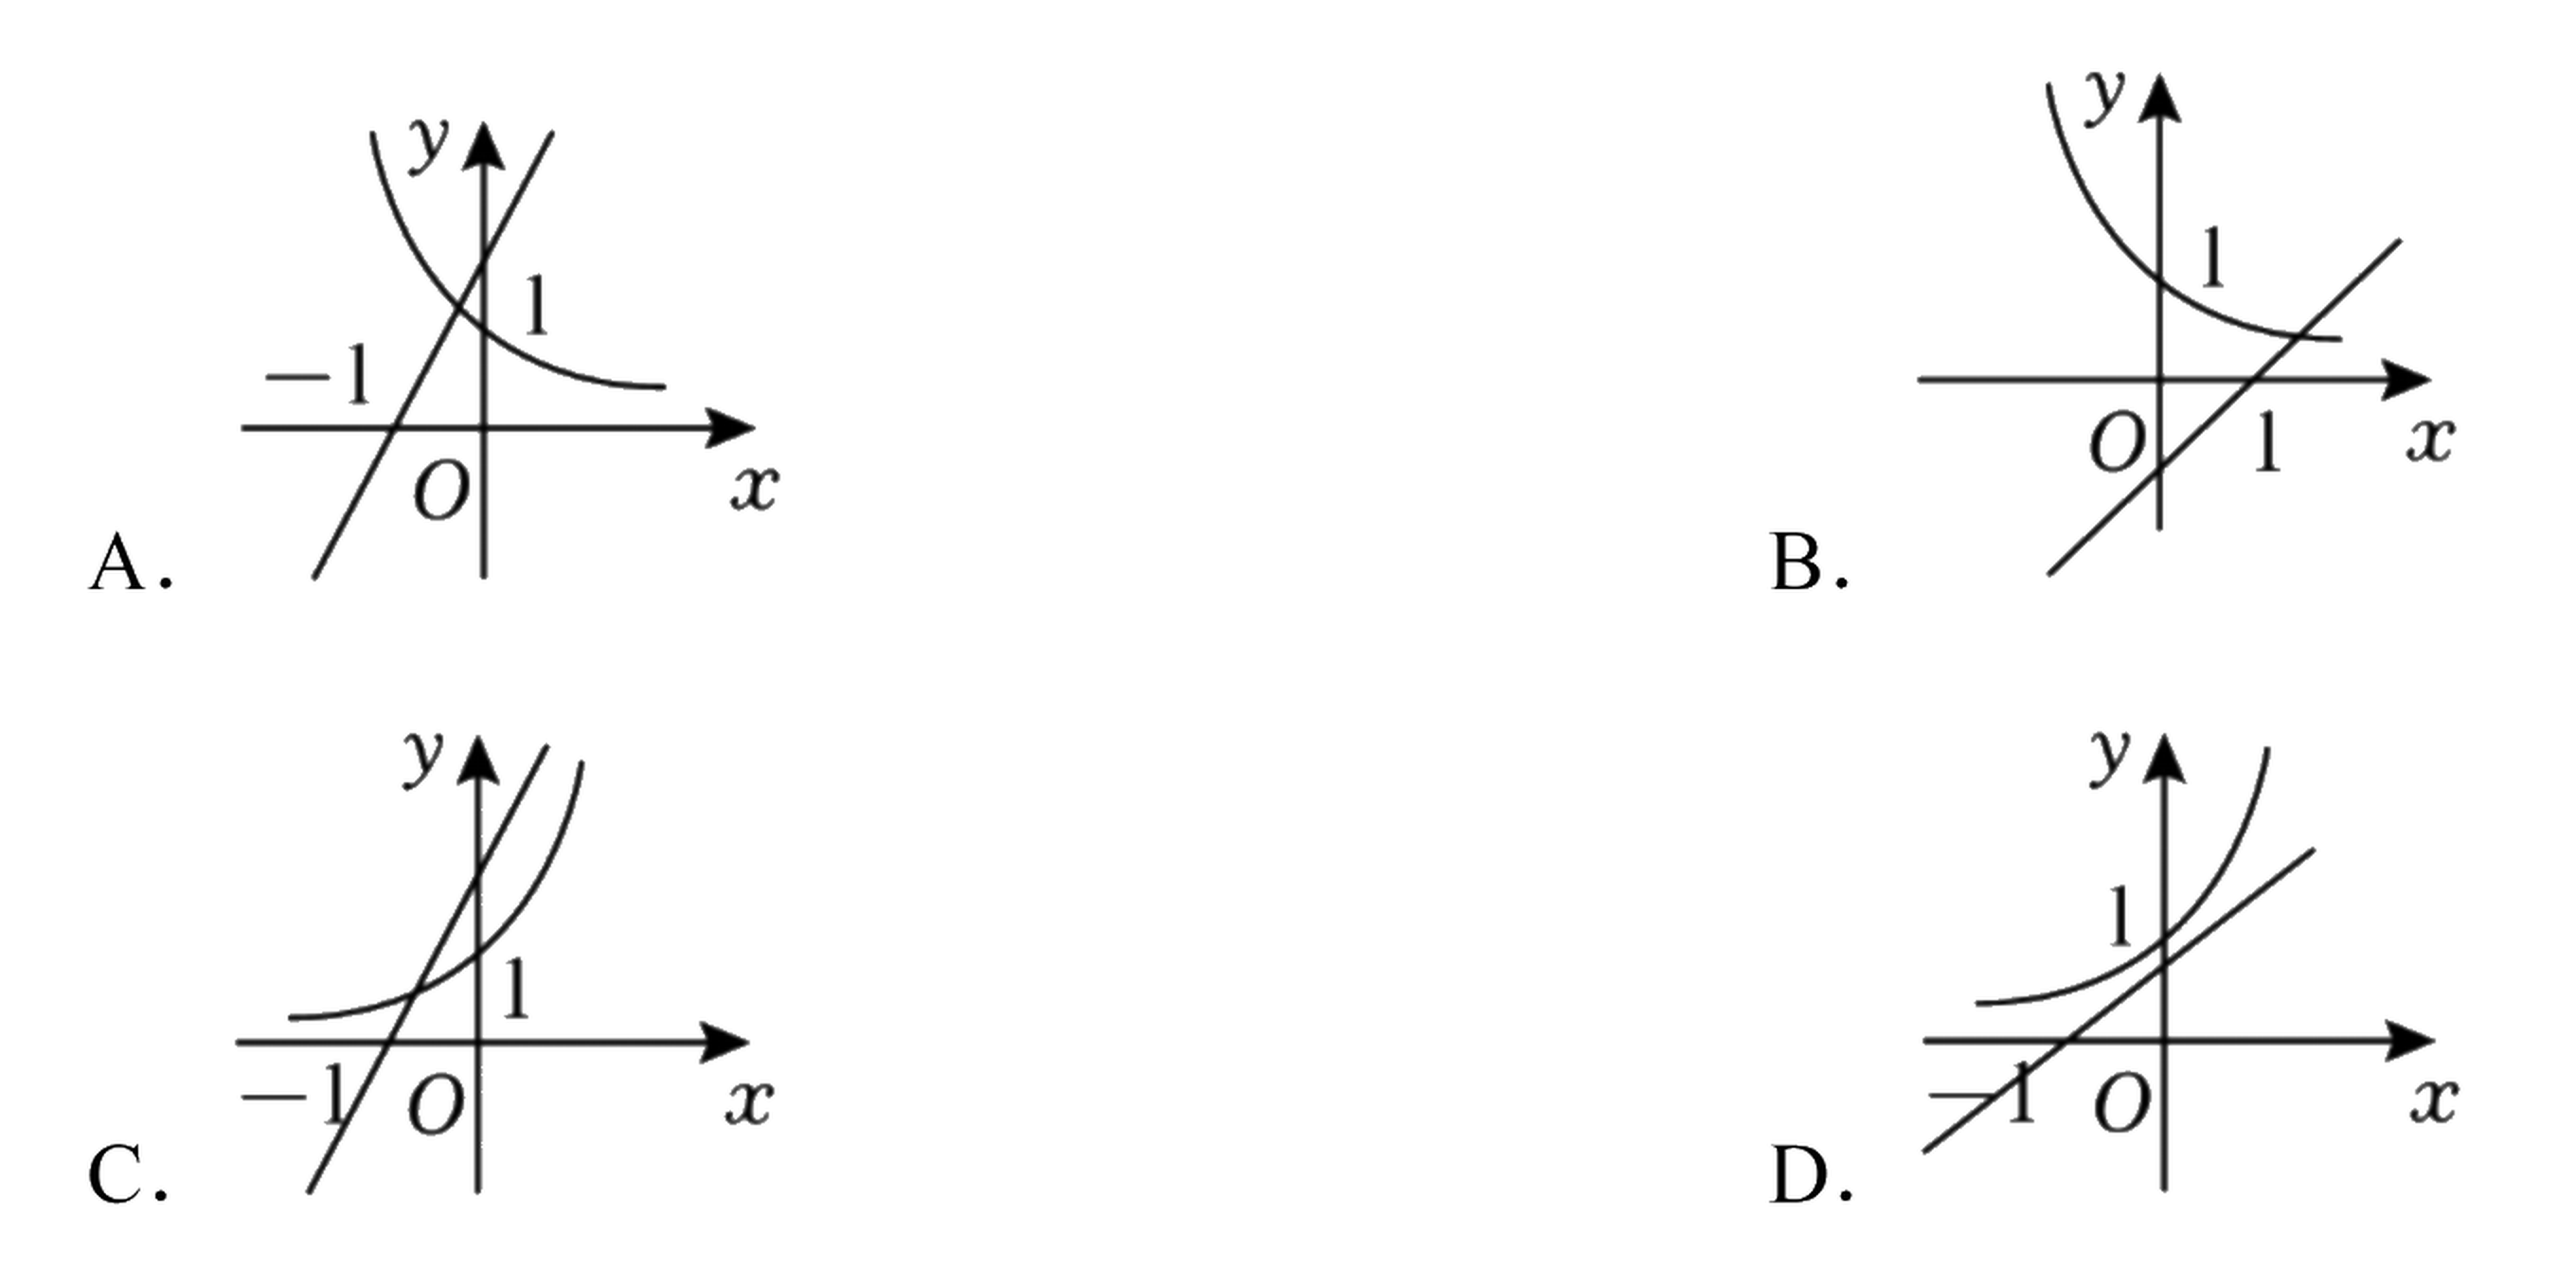
\includegraphics[width=0.80\textwidth]{figures/gao130_q15.png}
\end{center}

\ifanswer
\solbegin
\step{A 中，由指数函数 $y=a^x(a>0$ 且 $a\neq1)$ 图像递减得 $0<a<1$，}
\step{而一次函数 $y=a(x+1)$ 的图像与 $y$ 轴交点纵坐标为 $a>1$，二者矛盾，}
\step{所以 A 错；}
\step{由一次函数 $y=a(x+1)$ 的图像与 $x$ 轴交点横坐标为 $-1$，排除 B；}
\step{C 中，由指数函数 $y=a^x(a>0$ 且 $a\neq1)$ 图像递减得 $a>1$，}% 原卷"递减得 a>1"系笔误（应为"递增"），与 A 中"递减得 0<a<1"自相矛盾，照录
\step{而一次函数 $y=a(x+1)$ 的图像与 $y$ 轴交点纵坐标为 $a>1$，二者 $a$ 值吻合，}
\step{所以 C 对；}
\step{D 中，由一次函数 $y=a(x+1)$ 的图像得 $a=1$，与 $a>0$ 且 $a\neq1$ 矛盾，}
\step{所以 D 错.}
\step{故选 $C$.}
\solend
\fi

\item 设 $A_1$、$A_2$、$A_3$、$\cdots$、$A_7$ 是均含有 $2$ 个元素的集合，且 $A_1\cap A_7=\varnothing$，$A_i\cap A_{i+1}=\varnothing(i=1,2,3,\cdots,6)$，记 $B=A_1\cup A_2\cup A_3\cup\cdots\cup A_7$，则 $B$ 中元素个数的最小值是\mbox{（\quad）}

\keepwithprev
A. $4$\qquad B. $5$\qquad C. $6$\qquad D. $7$

\ifanswer
\solbegin
\step{取 $A_1=\{1,2\}$，$A_2=\{3,4\}$，$A_3=\{1,2\}$，$A_4=\{3,4\}$，$A_5=\{1,5\}$，$A_6=\{2,3\}$，$A_7=\{4,5\}$，}
\step{所以 $B$ 中元素个数的最小值是 $5$，故选 $B$.}
\solend
\fi

\end{enumerate}

\bigsec{三、解答题}

\begin{enumerate}
\setcounter{enumi}{16}

\item 已知全集为 $\R$，集合 $A=\{x\mid-2\leqslant x\leqslant5\}$，集合 $B=\{x\mid m-1\leqslant x\leqslant2m+1\}$．

(1) 求 $\overline{A}$；

(2) 若 $A\cup B=A$，求实数 $m$ 的取值范围．

\ifanswer
\solbegin
\step{(1) $(-\infty,-2)\cup(5,+\infty)$；}
\step{(2) 若 $A\cup B=A$，则 $B\subseteq A$，}
\step{当 $B=\varnothing$ 时，$m-1>2m+1$，解得 $m<-2$；}
\step{当 $B\neq\varnothing$ 时，$\begin{cases}m-1\leqslant2m+1\\m-1\geqslant-2\\2m+1\leqslant5\end{cases}$，解得 $-1\leqslant m\leqslant2$；}
\step{故实数 $m$ 的取值范围为 $\{m\mid-1\leqslant m\leqslant2$ 或 $m<-2\}$.}
\solend
\fi

\item 在不等式的应用中，有一些很基本而十分重要的不等式，如平均值不等式和三角不等式等，我们将其统称为基本不等式．

(1) 已知 $x$、$y$ 为正数，且 $2x+y=2$，求 $\dfrac1x+\dfrac2y$ 的最小值；

(2) 若关于 $x$ 的不等式 $\lvert x+1\rvert+\lvert2-x\rvert\geqslant a^2+a+1$ 对于一切实数 $x$ 都成立，求实数 $a$ 的取值范围．

\ifanswer
\solbegin
\step{(1) 因为 $x$、$y$ 为正数，且 $2x+y=2$，}
\step{所以 $\dfrac1x+\dfrac2y=\dfrac12\left(\dfrac1x+\dfrac2y\right)(2x+y)=\dfrac12\left(4+\dfrac yx+\dfrac{4x}y\right)\geqslant\dfrac12\left(4+2\sqrt{\dfrac yx\cdot\dfrac{4x}y}\right)=4$，}
\step{当且仅当 $\dfrac yx=\dfrac{4x}y$，即 $x=\dfrac12$，$y=1$ 时取等号，所以 $\dfrac1x+\dfrac2y$ 的最小值为 $4$；}
\step{(2) 由绝对值三角不等式得 $\lvert x+1\rvert+\lvert2-x\rvert\geqslant\lvert(x+1)+(2-x)\rvert=3$，}
\step{当且仅当 $-1\leqslant x\leqslant2$ 时取等号，所以 $\lvert x+1\rvert+\lvert2-x\rvert$ 的最小值为 $3$，}
\step{因为关于 $x$ 的不等式 $\lvert x+1\rvert+\lvert2-x\rvert\geqslant a^2+a+1$ 对于一切实数 $x$ 都成立，}
\step{所以 $a^2+a+1\leqslant3$，即 $a^2+a-2\leqslant0$，解得 $-2\leqslant a\leqslant1$，}
\step{所以实数 $a$ 的取值范围是 $[-2,1]$.}
\solend
\fi

\item 某医学专家为研究传染病传播中病毒细胞的发展规律，将病毒细胞注入一只小白鼠体内进行试验，经检测，病毒细胞的个数 $y$ 与天数 $x$ 的部分数据如表所示：

\begin{center}
\begin{tabular}{|c|c|c|c|c|c|c|c|}
\hline
天数 $(x)$ & $1$ & $2$ & $3$ & $4$ & $5$ & $6$ & $\cdots$ \\
\hline
病毒细胞的个数 $(y)$ & $1$ & $2$ & $4$ & $8$ & $16$ & $32$ & $\cdots$ \\
\hline
\end{tabular}
\end{center}

(1) 若病毒细胞的个数 $y$ 关于天数 $x$ 的变化规律可选用以下两个函数模型之一进行近似刻画：① $y=a\cdot b^x(a>0$，$b>0$，$b\neq1)$；② $y=a\cdot x^k(a\neq0)$．请结合表格中的数据，选择合适的函数模型，说明理由，并求出相应的函数表达式；

(2) 若该病毒细胞在小白鼠体内的个数超过 $10^8$，小白鼠将死亡，但注射某种药物，可杀死其体内 $98\%$ 的病毒细胞．则在 (1) 的条件下，为了使小白鼠在试验过程中不死亡，第一次最迟应在何时注射该种药物？（结果精确到天）

\ifanswer
\solbegin
\step{(1) 选择模型① $y=a\cdot b^x(a>0$，$b>0$，$b\neq1)$，理由如下：}
\step{观察表格数据，$y$ 的值随 $x$ 呈指数倍增：}
\step{$x=1$ 时，$y=1$，$x=2$ 时，$y=2$，$x=3$ 时，$y=4$，}
\step{后一天的病毒数是前一天的 $2$ 倍，符合指数增长的特征；}
\step{若选用幂函数模型 $y=a\cdot x^k$，代入前两组数据得 $a\cdot1^k=1$、$a\cdot2^k=2$，}
\step{解得 $a=1$，$k=1$，即 $y=x$，}
\step{但 $x=3$ 时，$y=3$ 与表格中 $y=4$ 严重不符，因此幂函数不匹配；}
\step{将 $(1,1)$ 代入 $y=a\cdot b^x$ 得 $a\cdot b=1$，}
\step{将 $(2,2)$ 代入得 $a\cdot b^2=2$，两式相除得 $b=2$，进而得 $a=\dfrac12$，}
\step{验证所有表格点均满足 $y=2^{x-1}$，最终函数表达式为 $y=2^{x-1}(x\in\N^*)$；}
\step{(2) 由题意得第一次注射药物前病毒细胞个数 $y$ 关于天数 $x(x\in\N^*)$ 的函数}
\step{关系式为 $y=2^{x-1}(x\in\N^*)$，}
\step{为了使小白鼠在试验过程中不死亡，则 $2^{x-1}\leqslant10^8$，}
\step{所以 $x-1\leqslant\log_210^8=8\log_210=\dfrac8{\lg2}$，解得 $x\leqslant1+\dfrac8{\lg2}\approx27.6$，}
\step{又 $x\in\N^*$，所以第一次最迟应在第 $27$ 天注射该种药物.}
\solend
\fi

\item 对在直角坐标系的第一象限内的任意两点 $(a,b)$，$(c,d)$ 作如下定义：$\dfrac ab>\dfrac cd$，那么称点 $(a,b)$ 是点 $(c,d)$ 的“上位点”，同时点 $(c,d)$ 是点 $(a,b)$ 的“下位点”．

(1) 试写出点 $(3,5)$ 的一个“上位点”坐标和一个“下位点”坐标；

(2) 设 $a$、$b$、$c$、$d$ 均为正数，且点 $(a,b)$ 是点 $(c,d)$ 的上位点，请判断点 $P(a+c,b+d)$ 是否既是点 $(a,b)$ 的“下位点”又是点 $(c,d)$ 的“上位点”，如果是，请证明；如果不是，请说明理由；

(3) 设正整数 $n$ 满足以下条件：对任意实数 $m\in\{t\mid0<t<4,t\in\Z\}$，总存在正整数 $k$，使得点 $(n,k)$ 既是点 $(4,m)$ 的“下位点”，又是点 $(5,m+1)$ 的“上位点”，求正整数 $n$ 的最小值．

\ifanswer
\solbegin
\step{(1) 由 $\dfrac34>\dfrac35>\dfrac36$ 得点 $(3,5)$ 的一个“上位点”的坐标为 $(3,4)$，}
\step{一个“下位点”的坐标为 $(3,6)$.}
\step{(2) 是，证明如下：}
\step{因为 $a$、$b$、$c$、$d$ 均为正数，点 $(a,b)$ 是点 $(c,d)$ 的“上位点”，}
\step{所以 $\dfrac ab>\dfrac cd$，所以 $ad>bc$，}
\step{因为 $\dfrac{a+c}{b+d}-\dfrac ab=\dfrac{b(a+c)-a(b+d)}{b(b+d)}=\dfrac{bc-ad}{b(b+d)}<0$，所以 $\dfrac{a+c}{b+d}<\dfrac ab$，}
\step{点 $P(a+c,b+d)$ 是点 $(a,b)$ 的“下位点”，}
\step{因为 $\dfrac{a+c}{b+d}-\dfrac cd=\dfrac{d(a+c)-c(b+d)}{d(b+d)}=\dfrac{ad-bc}{d(b+d)}>0$.}
\step{所以 $\dfrac{a+c}{b+d}>\dfrac cd$ 点 $P(a+c,b+d)$ 是点 $(c,d)$ 的“上位点”；}
\step{所以 $P(a+c,b+d)$ 既是点 $(a,b)$ 的“下位点”又是点 $(c,d)$ 的“上位点”；}
\step{(3) 由题意得 $m=1,2,3$，}
\step{由题意存在正整数 $k$：$\dfrac5{m+1}<\dfrac nk<\dfrac4m$，所以 $\begin{cases}\dfrac n4<k<\dfrac{2n}5(m=1)\\\dfrac n2<k<\dfrac{3n}5(m=2)\\\dfrac{3n}4<k<\dfrac{4n}5(m=3)\end{cases}$，}
\step{检验：$n=1,2,\cdots,8$ 不能同时找到整数 $k$，}
\step{$n=9$：$m=1$ 取 $k=3$，$m=2$ 取 $k=5$，$m=3$ 取 $k=7$，均满足，}
\step{所以正整数 $n$ 的最小值为 $9$.}
\solend
\fi

\end{enumerate}

\end{document}
"
%
% ① 原始材料：微信公众号"魔都数学加油站"文章，连载"27学年高一140"，原文标题
% "27学年高一140——2026-2027年上海市北郊高级中学高一上期中"；
% 原文链接：https://mp.weixin.qq.com/s/XBEYuTheiBoqu15dtLuD6A。
%   ★ 编号不一致说明：公众号连载号印"140"，与上一批已入库的"高一140 甘泉外国语"
%   （同一公众号另一篇文章、同为期中卷）撞号，系公众号笔误/重复。本仓库数字编号
%   02—143 中"高一130"一直空缺（连载 130 暂未见原文），故将本卷本地编号定为"高一130"、
%   填补该空缺，使数字编号连续（basename 全程为 高一130_北郊高级中学_期中）；
%   连载号 143 归正牌卷"上海中学 高一上期中"；本卷连载号仍印 140，见材料流转表。
%   卷面标题印"2026-2027 年北郊高级中学高一上期中"（卷面只有学校名、不含"上海市"、
%   不含任何期号/连载号），本稿照卷面录入；粉红色水印"魔都数学加油站"及页脚未录入。
% 正文为 9 张 PNG 页（01、04、05、06、09 为 2560x3620；02、03、07、08 为 4762x6735，
% 同一篇各页分辨率不同，逐页按各自分辨率放大核对），题目下印有【解析】，为讲评版。
% 题目、解析均据原图转录。
%
% 卷首标题：原卷印作"2026-2027 年北郊高级中学高一上期中"，年份区间按全稿惯例排
% en dash；原卷未印副标题，本卷为期中卷、跨集合与常用逻辑用语／不等式／函数三章，
% 按题目内容补出"集合与常用逻辑用语、不等式、函数"（与 125／126／128／129／131／132／133
% 同期中卷口径相同）。
%
% 题号体例：本卷共 18 题——一、填空题 3—12（10 题）、二、选择题 13—16（4 题）、
% 三、解答题 17—20（4 题）。三节分别 \setcounter{enumi}{2}／{12}／{16}。
% 原卷从第 3 题起、无第 1、2 题、**无第 21 题**（第 20 题解析续至 09 页，末行
% "所以正整数 n 的最小值为 9."，09 页下半页整片空白＋水印收尾、无第 10 页），本稿保留原题号。
%
% ② 与原卷的排版差异：
%   ① 原文从第 3 题起，本稿保留原题号；原卷止于第 20 题、无第 21 题、无附加题节；
%   ② 原卷每题下直接印【解析】，本稿按全稿惯例置于答案版；全卷 18 题均印【解析】、
%      无独立【答案】段，四道选择题答案在解析末句"故选 C／D／C／B"，括号
%      \mbox{（\quad）} 留空、不另提 \ans{}；全卷 0 处 \ans{}，答案版【解析】标记数 18＝题数；
%   ③ 原卷未印副标题，本稿按"知识模块"口径补出；
%   ④ 原卷填空横线按全稿惯例排为 \blankline[4.4em]；选择题括号排 \mbox{（\quad）}、
%      每个选项段前按惯例加 \keepwithprev；解答题不留作答区、不加 \anspace（讲评版）；
%   ⑤ 原卷数集排斜体 $R$／$N$，按全稿惯例改 \R／\N；空集记号 \varnothing；
%      绝对值排 \lvert…\rvert，集合描述竖线排 \mid；不等号按全稿惯例排 \leqslant／\geqslant；
%      补集照原卷上划线 \overline{A}；
%   ⑥ 1 幅插图 + 1 张印刷表格：第 15 题四幅坐标函数图象选项（04 页）取原卷截图
%      去粉色水印、去色、按原卷 2x2 排布合并为 figures/gao130_q15.png（非插图重绘），
%      放在 \keepwithprev 之后 \begin{center} 内、三版都出；第 19 题 (1) 印刷数据表格
%      （07 页，天数 x 1—6／病毒细胞个数 y 1/2/4/8/16/32）按原卷用 tabular 重排、
%      题干内三版都出（非插图）。
%      第 15 题是"二、选择题"节内带大图块的第三题（Q13 为节首题但无图），
%      在 \bigsec{二、选择题} 之前加 \needvspace{11cm} 连节标题一起量、Q15 \item 之前
%      加 \needvspace{9cm}——守卫必须放在 \bigsec 之前，放标题之后会让"二、选择题"
%      孤立在页末（B 类，照 高一26／40／59／136／140 成例）；三版切页审计均"合计异常：无"；
%   ⑦ 子题标号 (1)(2)(3) 原卷用半角括号，照录；圈数字 ①②③④ 照录；
%      数学式内半角逗号照录（如第 14 题 $(a>0,a\neq1)$、第 16 题
%      $(i=1,2,3,\cdots,6)$、第 20 题 $m=1,2,3$ 等）；
%      行末西文句点按全稿惯例照录；
%   ⑧ 题干中的中文弯引号按原卷照录（Q12"变项和"、Q20"上位点""下位点"等），
%      注释内一律 ASCII 引号；原卷"图像"用词逐处照录（Q9、Q15 均作"图像"）。
%
% ③ 行数复核：一条 \step = 原卷解析的一个印刷行（cases 块与 tabular 各作一个印刷行计）。
%   逐题 \step 条数，合计 98 条（Q3:3 Q4:2 Q5:2 Q6:1 Q7:1 Q8:3 Q9:5 Q10:10 Q11:6
%   Q12:7 Q13:1 Q14:2 Q15:10 Q16:2 Q17:5 Q18:8 Q19:15 Q20:15），与原卷印刷行逐题相等。
%
% ④ 判别式／子集符号结论：
%   判别式：全卷未出现判别式记号（无 $\Delta$、无 $\triangle$）；
%   子集符号：第 4 题题干"$B\subseteq A$"、第 4 题【解析】"$B\subseteq A$"、
%      第 17 题 (2)【解析】"$B\subseteq A$"三处原卷均印带下划线 $\subseteq$，逐处
%      放大核对、照录 \subseteq；全卷未出现单线 \subset。
%
% ⑤ 原卷存疑照录（均照录未改，正文对应处另有 % 注）：
%   ① 第 15 题【解析】"C 中，由指数函数 $y=a^x$ 图像递减得 $a>1$"——"递减"应为
%      "递增"之误（与同题 A 中"递减得 $0<a<1$"自相矛盾），原卷如此，照录并加注；
%   ② 第 16 题题干"$A_1\cap A_7=\varnothing$""$A_i\cap A_{i+1}=\varnothing$"
%      的空集记号与解析所列各集合逐处照录；
%   ③ 第 19 题 (2) 题干"可杀死其体内 98% 的病毒细胞"、解析 (2) 只按 $y=2^{x-1}$
%      与 $10^8$ 比较（未另计 98%），照录不补步。
%
% ⑥ 跨页续印按题合并：Q8 题干在 01 页末、解析在 02 页；Q9 题干在 02 页、
%   解析在 02 页；Q10 题干在 02 页、解析前 5 行在 02—03 页、后 5 行在 03 页；
%   Q12 题干跨 03 页、解析首 5 行在 03 页末、末行在 04 页；Q15 题干在 04 页、
%   四幅图与解析前段在 04 页、解析续在 05 页；Q17 解析跨 05—06 页；Q18 题干与
%   (1) 解析在 06 页、(2) 解析在 06—07 页；Q19 表格在 07 页、解析跨 07—08 页；
%   Q20 定义与三小问在 08 页、解析 (1)(2) 在 08—09 页、解析 (3) 在 09 页；
%   本稿按题连排，不丢行。
%
\documentclass[a4paper,11pt]{article}
\usepackage{common}

\begin{document}

\examtitlest[3]{2026--2027 年北郊高级中学高一上期中}{集合与常用逻辑用语、不等式、函数}

\bigsec{一、填空题}

\begin{enumerate}
\setcounter{enumi}{2}

\item 不等式 $\dfrac{x-3}{x+1}<2$ 的解集为\blankline[4.4em].

\ifanswer
\solbegin
\step{不等式 $\dfrac{x-3}{x+1}<2$ 可化为 $\dfrac{x-3}{x+1}-2<0$，即 $\dfrac{x-3-2(x+1)}{x+1}<0$，}
\step{化简为 $\dfrac{x+5}{x+1}>0$，解得 $x<-5$ 或 $x>-1$，}
\step{所以不等式的解集为 $\{x\mid x<-5$ 或 $x>-1\}$.}
\solend
\fi

\item 已知集合 $A=\{x\mid0<x<a\}$，$B=\{x\mid1<x<2\}$，若 $B\subseteq A$，则实数 $a$ 的取值范围为\blankline[4.4em].

\ifanswer
\solbegin
\step{已知集合 $A=\{x\mid0<x<a\}$，$B=\{x\mid1<x<2\}$，}
\step{若 $B\subseteq A$，则 $a\geqslant2$，所以实数 $a$ 的取值范围是 $\{a\mid a\geqslant2\}$.}
\solend
\fi

\item 已知关于 $x$ 的方程 $x^2+x+c=0$ 的两个实数根为 $x_1$、$x_2$，若 $x_1^2x_2+x_2^2x_1=3$，则实数 $c=$\blankline[4.4em].

\ifanswer
\solbegin
\step{由韦达定理得 $x_1+x_2=-1$，$x_1x_2=c$，所以 $x_1^2x_2+x_2^2x_1=(x_1+x_2)x_1x_2=-c=3$，}
\step{所以 $c=-3$.}
\solend
\fi

\item 已知 $10^x=3$，$10^y=64$，则 $10^{x-\frac y3}=$\blankline[4.4em].

\ifanswer
\solbegin
\step{$10^{x-\frac y3}=10^x\div\sqrt[3]{10^y}=\dfrac34$.}
\solend
\fi

\item 若 $\lg2=a$，则可用 $a$ 表示 $\log_280=$\blankline[4.4em].

\ifanswer
\solbegin
\step{$\log_280=\dfrac{\lg80}{\lg2}=\dfrac{\lg10+\lg8}{\lg2}=\dfrac{1+3\lg2}{\lg2}=\dfrac{1+3a}{a}$.}
\solend
\fi

\item 已知 $a+2b=1$，则 $3^a+9^b$ 的最小值为\blankline[4.4em].

\ifanswer
\solbegin
\step{因为 $a+2b=1$，所以 $3^a+9^b=3^a+3^{2b}\geqslant2\sqrt{3^a\cdot3^{2b}}=2\sqrt{3^{a+2b}}=2\sqrt3$，}
\step{当且仅当 $3^a=3^{2b}$，且 $a+2b=1$，即 $a=\dfrac12$，$b=\dfrac14$ 时取等号，}
\step{故最小值为 $2\sqrt3$.}
\solend
\fi

\item 下列函数的图像关于原点成中心对称，且在区间 $(0,+\infty)$ 上是严格增函数的是\blankline[4.4em]（请填写全部正确的序号）.

① $y=\sqrt{x}$；② $y=\sqrt[3]{x}$；③ $y=x^{\frac23}$；④ $y=x^{-\frac13}$.

\ifanswer
\solbegin
\step{① $y=\sqrt{x}$ 的定义域为 $[0,+\infty)$，故其图像不关于原点成中心对称，①错误；}
\step{② $y=\sqrt[3]{x}$ 是奇函数，且在区间 $(0,+\infty)$ 上是严格增函数，②正确；}
\step{③ $y=x^{\frac23}$ 是偶函数，其图像关于 $y$ 轴对称，不关于原点成中心对称，③错误；}
\step{④由于幂指数 $-\dfrac13<0$，故 $y=x^{-\frac13}$ 在区间 $(0,+\infty)$ 上是严格减函数，④错误.}
\step{故正确的是②.}
\solend
\fi

\item 设 $a>0$ 且 $a\neq1$，若函数 $y=a^{2x}+2a^x-3$ 在区间 $[-1,1]$ 上的最大值为 $21$，则实数 $a$ 的值为\blankline[4.4em].

\ifanswer
\solbegin
\step{令 $t=a^x$，$x\in[-1,1]$，}
\step{当 $a>1$ 时，$t=a^x$ 严格增，则 $t\in\left[\dfrac1a,a\right]$，}
\step{则函数 $y=t^2+2t-3$，对称轴为 $t=-1$，}
\step{所以函数 $y=t^2+2t-3$ 在 $\left[\dfrac1a,a\right]$ 上严格增，}
\step{所以当 $t=a$ 时，$y$ 取得最大值 $a^2+2a-3=21$，解得 $a=4$ 或 $-6$（舍去）；}
\step{当 $0<a<1$ 时，$t=a^x$ 严格减，则 $t\in\left[a,\dfrac1a\right]$，}
\step{则函数 $y=t^2+2t-3$，对称轴为 $t=-1$，}
\step{所以函数 $y=t^2+2t-3$ 在 $\left[a,\dfrac1a\right]$ 上严格增，}
\step{所以当 $t=\dfrac1a$ 时，$y$ 取得最大值 $\dfrac1{a^2}+\dfrac2a-3=21$，解得 $a=\dfrac14$ 或 $-\dfrac16$（舍去）；}
\step{综上所述，实数 $a$ 的值为 $4$ 或 $\dfrac14$.}
\solend
\fi

\item 在关于 $x$ 的不等式 $x^2+(m+1)x+m<0$ 的解集中恰有两个整数，则实数 $m$ 的取值范围是\blankline[4.4em].

\ifanswer
\solbegin
\step{关于 $x$ 的不等式 $x^2+(m+1)x+m<0$ 可化为 $(x+1)(x+m)<0$，}
\step{当 $m>1$ 时，$-m<-1$，解不等式得 $-m<x<-1$；}
\step{当 $m<1$ 时，$-m>-1$，解不等式得 $-1<x<-m$；}
\step{由不等式的解集中恰有两个整数，}
\step{则 $-4\leqslant-m<-3$ 或 $1<-m\leqslant2$，即 $3<m\leqslant4$ 或 $-2\leqslant m<-1$，}
\step{所以 $m$ 的取值范围是 $[-2,-1)\cup(3,4]$.}
\solend
\fi

\item 已知集合 $M$ 的元素均为正整数，定义集合 $M$ 的“变项和”为：将 $M$ 中每个元素 $m$ 都乘以 $(-1)^m$ 后再求和．若集合 $A=\{n\mid1\leqslant n\leqslant20,n\in\N\}$，则集合 $A$ 的所有非空子集的“变项和”的总和为\blankline[4.4em].

\ifanswer
\solbegin
\step{集合 $A=\{n\mid1\leqslant n\leqslant20,n\in\N\}$ 中一共有 $20$ 个元素，}
\step{固定选中 $k$，剩下 $19$ 个元素任选，共 $2^{19}$ 个子集包含 $k$，每个 $k$ 贡献 $(-1)^k\cdot k\cdot2^{19}$，}
\step{$A=\{1,2,\cdots,20\}$，}
\step{奇数 $k=1,3,\cdots,19$，共 $10$ 个，$(-1)^k\cdot k=-k$，}
\step{偶数 $k=2,4,\cdots,20$，共 $10$ 个，$(-1)^k\cdot k=k$，}
\step{所以集合 $A$ 的所有非空子集的“变项和”的总和}
\step{为 $S=2^{19}\times[(-1+2)+(-3+4)+\cdots+(-19+20)]=2^{19}\times10=524880$.}
\solend
\fi

\end{enumerate}

% 第 15 题四幅图是"二、选择题"节内大图块；守卫须放在 \bigsec 之前连节标题一起量，
% 否则"二、选择题"会孤立在页末（B 类，照 高一26／40／59／136／140 成例）
\needvspace{11cm}
\bigsec{二、选择题}

\begin{enumerate}
\setcounter{enumi}{12}

\item 设 $ab>0$，则“$a>b$”是“$\dfrac1a<\dfrac1b$”的\mbox{（\quad）}

\keepwithprev
A. 充分非必要条件\qquad B. 必要非充分条件

C. 充要条件\qquad D. 既非充分也非必要条件

\ifanswer
\solbegin
\step{因为 $ab>0$，所以 $a>b\Leftrightarrow\dfrac1a<\dfrac1b$，故选 $C$.}
\solend
\fi

\item 已知 $A=\log_ax$，$B=\log_ay(a>0,a\neq1)$，则 $\log_a\dfrac{x^2}{\sqrt y}=$\mbox{（\quad）}

\keepwithprev
A. $\dfrac{A^2}{\sqrt B}$\qquad B. $2A^2B$\qquad C. $4AB$\qquad D. $2A-\dfrac12B$

\ifanswer
\solbegin
\step{由已知得 $x=a^A$，$y=a^B$，}
\step{所以 $\log_a\dfrac{x^2}{\sqrt y}=\log_a\dfrac{(a^A)^2}{\sqrt{a^B}}=\log_a\dfrac{a^{2A}}{a^{\frac12B}}=\log_a a^{2A-\frac12B}=2A-\dfrac12B$. 故选 $D$.}
\solend
\fi

% 第 15 题四幅坐标函数图象选项是一整块，守卫放在 \item 之前
\needvspace{9cm}
\item 在同一平面直角坐标系中，指数函数 $y=a^x(a>0$ 且 $a\neq1)$ 和一次函数 $y=a(x+1)$ 的图像关系可能是\mbox{（\quad）}

\keepwithprev
\begin{center}
% 四幅坐标函数图象选项取原卷 04 页截图去粉色水印、去色，按原卷 2x2 排布合并为一张
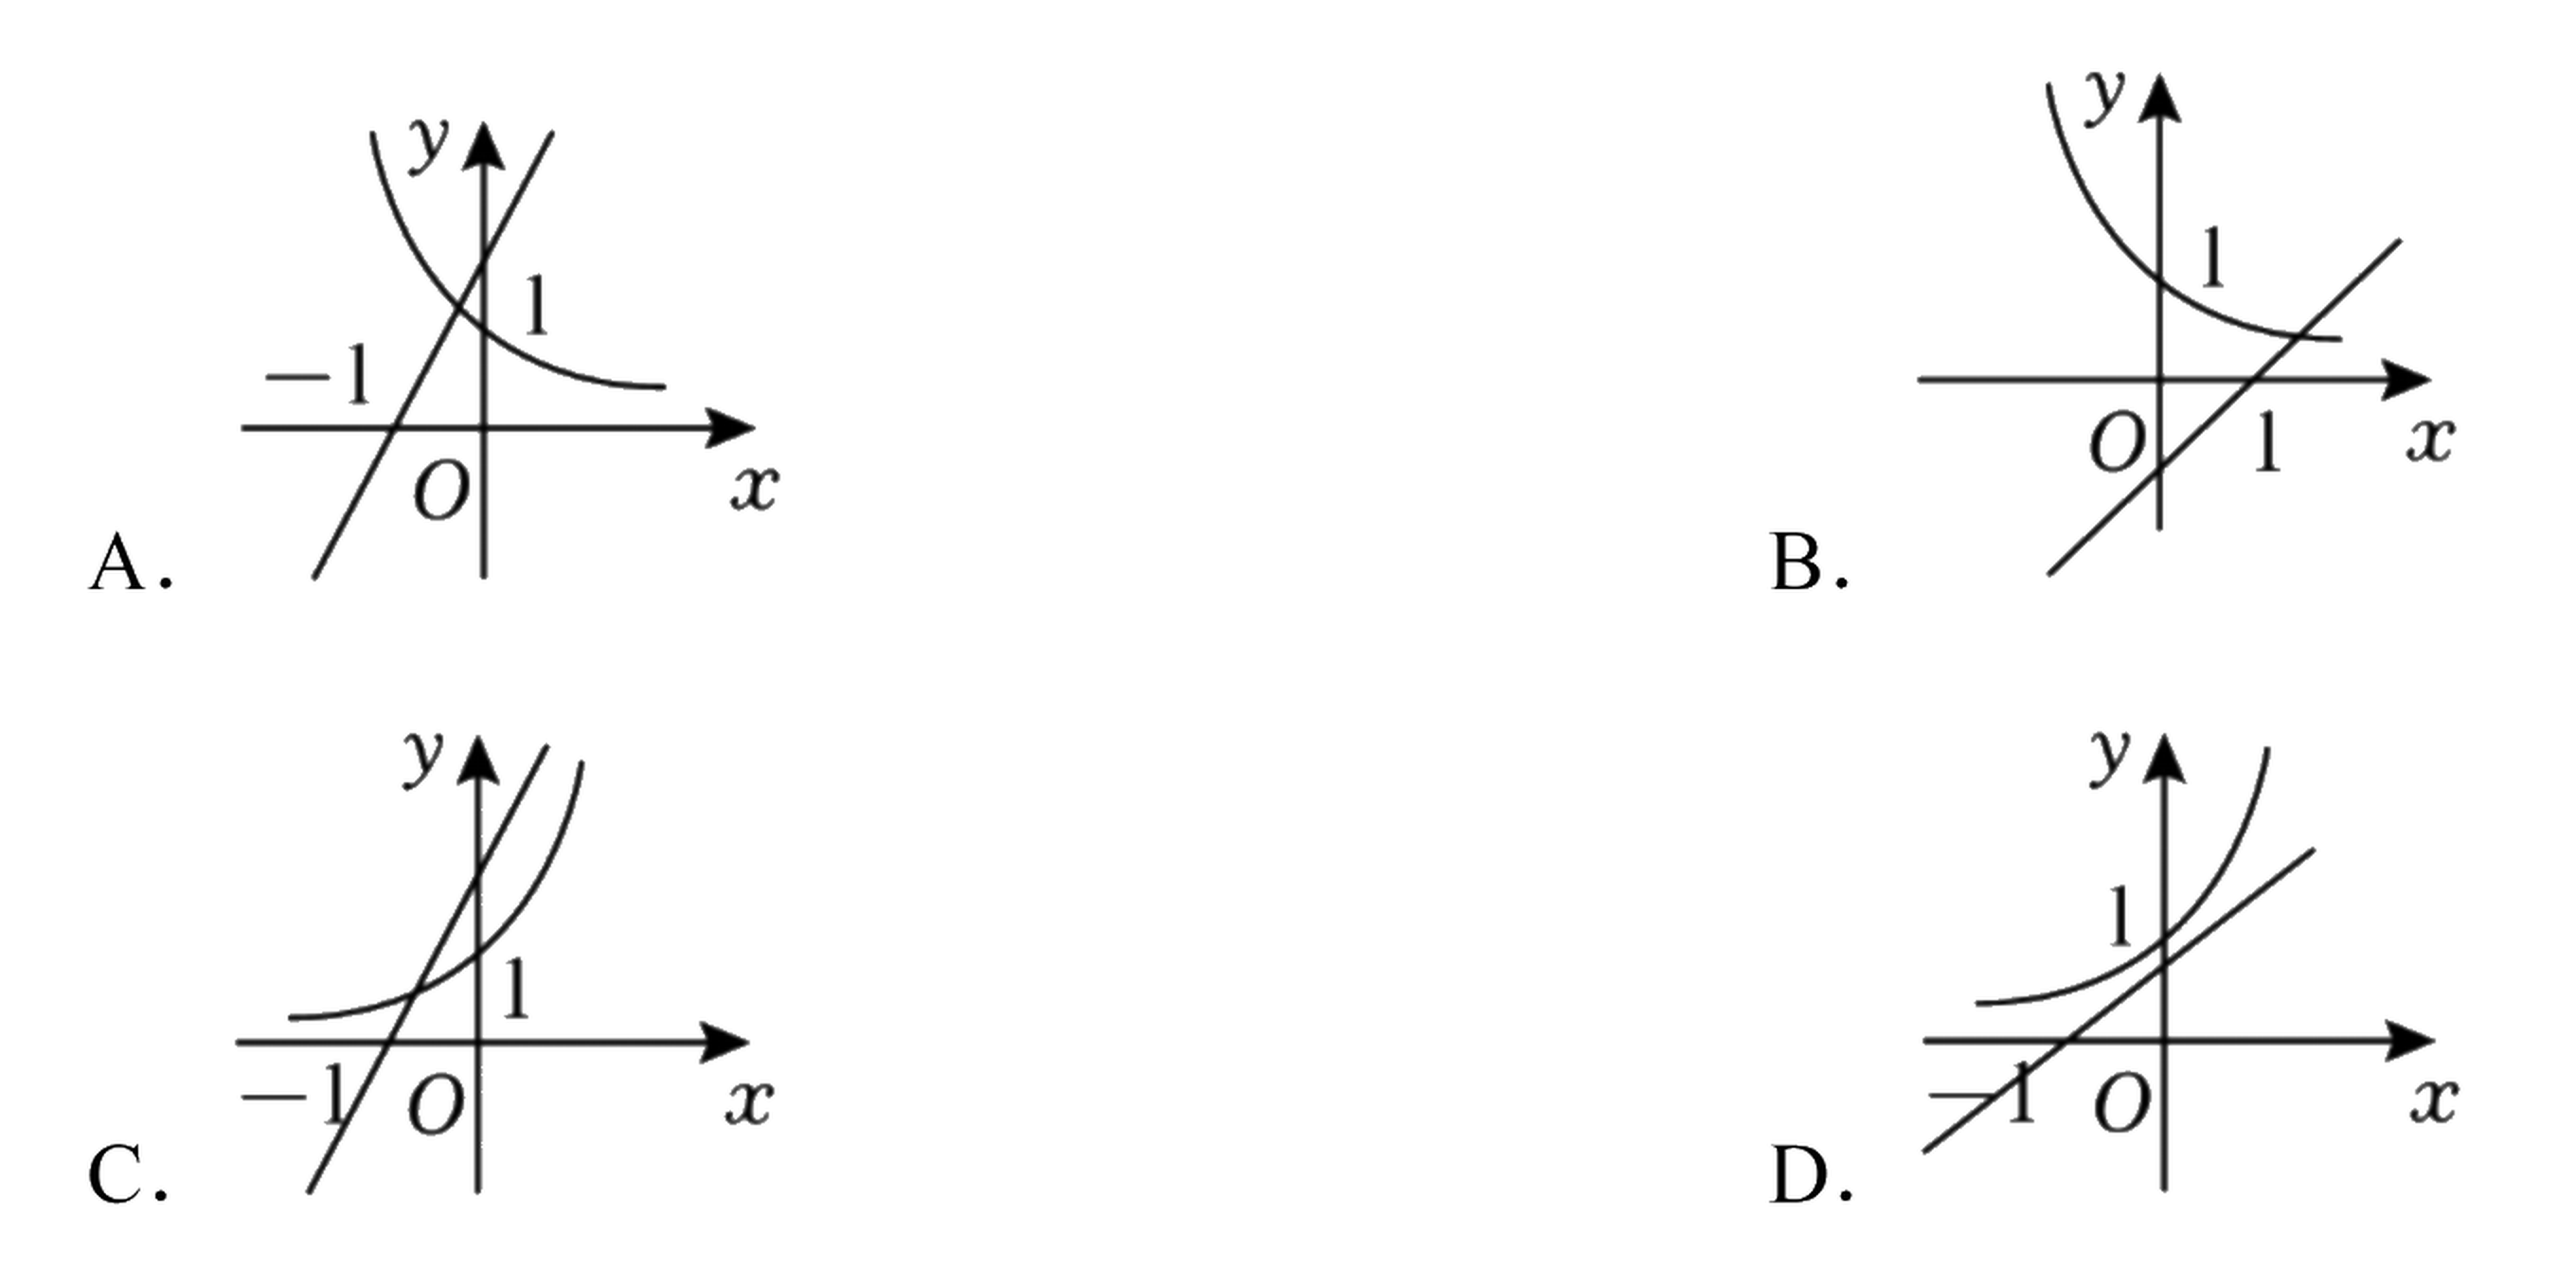
\includegraphics[width=0.80\textwidth]{figures/gao130_q15.png}
\end{center}

\ifanswer
\solbegin
\step{A 中，由指数函数 $y=a^x(a>0$ 且 $a\neq1)$ 图像递减得 $0<a<1$，}
\step{而一次函数 $y=a(x+1)$ 的图像与 $y$ 轴交点纵坐标为 $a>1$，二者矛盾，}
\step{所以 A 错；}
\step{由一次函数 $y=a(x+1)$ 的图像与 $x$ 轴交点横坐标为 $-1$，排除 B；}
\step{C 中，由指数函数 $y=a^x(a>0$ 且 $a\neq1)$ 图像递减得 $a>1$，}% 原卷"递减得 a>1"系笔误（应为"递增"），与 A 中"递减得 0<a<1"自相矛盾，照录
\step{而一次函数 $y=a(x+1)$ 的图像与 $y$ 轴交点纵坐标为 $a>1$，二者 $a$ 值吻合，}
\step{所以 C 对；}
\step{D 中，由一次函数 $y=a(x+1)$ 的图像得 $a=1$，与 $a>0$ 且 $a\neq1$ 矛盾，}
\step{所以 D 错.}
\step{故选 $C$.}
\solend
\fi

\item 设 $A_1$、$A_2$、$A_3$、$\cdots$、$A_7$ 是均含有 $2$ 个元素的集合，且 $A_1\cap A_7=\varnothing$，$A_i\cap A_{i+1}=\varnothing(i=1,2,3,\cdots,6)$，记 $B=A_1\cup A_2\cup A_3\cup\cdots\cup A_7$，则 $B$ 中元素个数的最小值是\mbox{（\quad）}

\keepwithprev
A. $4$\qquad B. $5$\qquad C. $6$\qquad D. $7$

\ifanswer
\solbegin
\step{取 $A_1=\{1,2\}$，$A_2=\{3,4\}$，$A_3=\{1,2\}$，$A_4=\{3,4\}$，$A_5=\{1,5\}$，$A_6=\{2,3\}$，$A_7=\{4,5\}$，}
\step{所以 $B$ 中元素个数的最小值是 $5$，故选 $B$.}
\solend
\fi

\end{enumerate}

\bigsec{三、解答题}

\begin{enumerate}
\setcounter{enumi}{16}

\item 已知全集为 $\R$，集合 $A=\{x\mid-2\leqslant x\leqslant5\}$，集合 $B=\{x\mid m-1\leqslant x\leqslant2m+1\}$．

(1) 求 $\overline{A}$；

(2) 若 $A\cup B=A$，求实数 $m$ 的取值范围．

\ifanswer
\solbegin
\step{(1) $(-\infty,-2)\cup(5,+\infty)$；}
\step{(2) 若 $A\cup B=A$，则 $B\subseteq A$，}
\step{当 $B=\varnothing$ 时，$m-1>2m+1$，解得 $m<-2$；}
\step{当 $B\neq\varnothing$ 时，$\begin{cases}m-1\leqslant2m+1\\m-1\geqslant-2\\2m+1\leqslant5\end{cases}$，解得 $-1\leqslant m\leqslant2$；}
\step{故实数 $m$ 的取值范围为 $\{m\mid-1\leqslant m\leqslant2$ 或 $m<-2\}$.}
\solend
\fi

\item 在不等式的应用中，有一些很基本而十分重要的不等式，如平均值不等式和三角不等式等，我们将其统称为基本不等式．

(1) 已知 $x$、$y$ 为正数，且 $2x+y=2$，求 $\dfrac1x+\dfrac2y$ 的最小值；

(2) 若关于 $x$ 的不等式 $\lvert x+1\rvert+\lvert2-x\rvert\geqslant a^2+a+1$ 对于一切实数 $x$ 都成立，求实数 $a$ 的取值范围．

\ifanswer
\solbegin
\step{(1) 因为 $x$、$y$ 为正数，且 $2x+y=2$，}
\step{所以 $\dfrac1x+\dfrac2y=\dfrac12\left(\dfrac1x+\dfrac2y\right)(2x+y)=\dfrac12\left(4+\dfrac yx+\dfrac{4x}y\right)\geqslant\dfrac12\left(4+2\sqrt{\dfrac yx\cdot\dfrac{4x}y}\right)=4$，}
\step{当且仅当 $\dfrac yx=\dfrac{4x}y$，即 $x=\dfrac12$，$y=1$ 时取等号，所以 $\dfrac1x+\dfrac2y$ 的最小值为 $4$；}
\step{(2) 由绝对值三角不等式得 $\lvert x+1\rvert+\lvert2-x\rvert\geqslant\lvert(x+1)+(2-x)\rvert=3$，}
\step{当且仅当 $-1\leqslant x\leqslant2$ 时取等号，所以 $\lvert x+1\rvert+\lvert2-x\rvert$ 的最小值为 $3$，}
\step{因为关于 $x$ 的不等式 $\lvert x+1\rvert+\lvert2-x\rvert\geqslant a^2+a+1$ 对于一切实数 $x$ 都成立，}
\step{所以 $a^2+a+1\leqslant3$，即 $a^2+a-2\leqslant0$，解得 $-2\leqslant a\leqslant1$，}
\step{所以实数 $a$ 的取值范围是 $[-2,1]$.}
\solend
\fi

\item 某医学专家为研究传染病传播中病毒细胞的发展规律，将病毒细胞注入一只小白鼠体内进行试验，经检测，病毒细胞的个数 $y$ 与天数 $x$ 的部分数据如表所示：

\begin{center}
\begin{tabular}{|c|c|c|c|c|c|c|c|}
\hline
天数 $(x)$ & $1$ & $2$ & $3$ & $4$ & $5$ & $6$ & $\cdots$ \\
\hline
病毒细胞的个数 $(y)$ & $1$ & $2$ & $4$ & $8$ & $16$ & $32$ & $\cdots$ \\
\hline
\end{tabular}
\end{center}

(1) 若病毒细胞的个数 $y$ 关于天数 $x$ 的变化规律可选用以下两个函数模型之一进行近似刻画：① $y=a\cdot b^x(a>0$，$b>0$，$b\neq1)$；② $y=a\cdot x^k(a\neq0)$．请结合表格中的数据，选择合适的函数模型，说明理由，并求出相应的函数表达式；

(2) 若该病毒细胞在小白鼠体内的个数超过 $10^8$，小白鼠将死亡，但注射某种药物，可杀死其体内 $98\%$ 的病毒细胞．则在 (1) 的条件下，为了使小白鼠在试验过程中不死亡，第一次最迟应在何时注射该种药物？（结果精确到天）

\ifanswer
\solbegin
\step{(1) 选择模型① $y=a\cdot b^x(a>0$，$b>0$，$b\neq1)$，理由如下：}
\step{观察表格数据，$y$ 的值随 $x$ 呈指数倍增：}
\step{$x=1$ 时，$y=1$，$x=2$ 时，$y=2$，$x=3$ 时，$y=4$，}
\step{后一天的病毒数是前一天的 $2$ 倍，符合指数增长的特征；}
\step{若选用幂函数模型 $y=a\cdot x^k$，代入前两组数据得 $a\cdot1^k=1$、$a\cdot2^k=2$，}
\step{解得 $a=1$，$k=1$，即 $y=x$，}
\step{但 $x=3$ 时，$y=3$ 与表格中 $y=4$ 严重不符，因此幂函数不匹配；}
\step{将 $(1,1)$ 代入 $y=a\cdot b^x$ 得 $a\cdot b=1$，}
\step{将 $(2,2)$ 代入得 $a\cdot b^2=2$，两式相除得 $b=2$，进而得 $a=\dfrac12$，}
\step{验证所有表格点均满足 $y=2^{x-1}$，最终函数表达式为 $y=2^{x-1}(x\in\N^*)$；}
\step{(2) 由题意得第一次注射药物前病毒细胞个数 $y$ 关于天数 $x(x\in\N^*)$ 的函数}
\step{关系式为 $y=2^{x-1}(x\in\N^*)$，}
\step{为了使小白鼠在试验过程中不死亡，则 $2^{x-1}\leqslant10^8$，}
\step{所以 $x-1\leqslant\log_210^8=8\log_210=\dfrac8{\lg2}$，解得 $x\leqslant1+\dfrac8{\lg2}\approx27.6$，}
\step{又 $x\in\N^*$，所以第一次最迟应在第 $27$ 天注射该种药物.}
\solend
\fi

\item 对在直角坐标系的第一象限内的任意两点 $(a,b)$，$(c,d)$ 作如下定义：$\dfrac ab>\dfrac cd$，那么称点 $(a,b)$ 是点 $(c,d)$ 的“上位点”，同时点 $(c,d)$ 是点 $(a,b)$ 的“下位点”．

(1) 试写出点 $(3,5)$ 的一个“上位点”坐标和一个“下位点”坐标；

(2) 设 $a$、$b$、$c$、$d$ 均为正数，且点 $(a,b)$ 是点 $(c,d)$ 的上位点，请判断点 $P(a+c,b+d)$ 是否既是点 $(a,b)$ 的“下位点”又是点 $(c,d)$ 的“上位点”，如果是，请证明；如果不是，请说明理由；

(3) 设正整数 $n$ 满足以下条件：对任意实数 $m\in\{t\mid0<t<4,t\in\Z\}$，总存在正整数 $k$，使得点 $(n,k)$ 既是点 $(4,m)$ 的“下位点”，又是点 $(5,m+1)$ 的“上位点”，求正整数 $n$ 的最小值．

\ifanswer
\solbegin
\step{(1) 由 $\dfrac34>\dfrac35>\dfrac36$ 得点 $(3,5)$ 的一个“上位点”的坐标为 $(3,4)$，}
\step{一个“下位点”的坐标为 $(3,6)$.}
\step{(2) 是，证明如下：}
\step{因为 $a$、$b$、$c$、$d$ 均为正数，点 $(a,b)$ 是点 $(c,d)$ 的“上位点”，}
\step{所以 $\dfrac ab>\dfrac cd$，所以 $ad>bc$，}
\step{因为 $\dfrac{a+c}{b+d}-\dfrac ab=\dfrac{b(a+c)-a(b+d)}{b(b+d)}=\dfrac{bc-ad}{b(b+d)}<0$，所以 $\dfrac{a+c}{b+d}<\dfrac ab$，}
\step{点 $P(a+c,b+d)$ 是点 $(a,b)$ 的“下位点”，}
\step{因为 $\dfrac{a+c}{b+d}-\dfrac cd=\dfrac{d(a+c)-c(b+d)}{d(b+d)}=\dfrac{ad-bc}{d(b+d)}>0$.}
\step{所以 $\dfrac{a+c}{b+d}>\dfrac cd$ 点 $P(a+c,b+d)$ 是点 $(c,d)$ 的“上位点”；}
\step{所以 $P(a+c,b+d)$ 既是点 $(a,b)$ 的“下位点”又是点 $(c,d)$ 的“上位点”；}
\step{(3) 由题意得 $m=1,2,3$，}
\step{由题意存在正整数 $k$：$\dfrac5{m+1}<\dfrac nk<\dfrac4m$，所以 $\begin{cases}\dfrac n4<k<\dfrac{2n}5(m=1)\\\dfrac n2<k<\dfrac{3n}5(m=2)\\\dfrac{3n}4<k<\dfrac{4n}5(m=3)\end{cases}$，}
\step{检验：$n=1,2,\cdots,8$ 不能同时找到整数 $k$，}
\step{$n=9$：$m=1$ 取 $k=3$，$m=2$ 取 $k=5$，$m=3$ 取 $k=7$，均满足，}
\step{所以正整数 $n$ 的最小值为 $9$.}
\solend
\fi

\end{enumerate}

\end{document}
"
%
% ① 原始材料：微信公众号"魔都数学加油站"文章，连载"27学年高一140"，原文标题
% "27学年高一140——2026-2027年上海市北郊高级中学高一上期中"；
% 原文链接：https://mp.weixin.qq.com/s/XBEYuTheiBoqu15dtLuD6A。
%   ★ 编号不一致说明：公众号连载号印"140"，与上一批已入库的"高一140 甘泉外国语"
%   （同一公众号另一篇文章、同为期中卷）撞号，系公众号笔误/重复。本仓库数字编号
%   02—143 中"高一130"一直空缺（连载 130 暂未见原文），故将本卷本地编号定为"高一130"、
%   填补该空缺，使数字编号连续（basename 全程为 高一130_北郊高级中学_期中）；
%   连载号 143 归正牌卷"上海中学 高一上期中"；本卷连载号仍印 140，见材料流转表。
%   卷面标题印"2026-2027 年北郊高级中学高一上期中"（卷面只有学校名、不含"上海市"、
%   不含任何期号/连载号），本稿照卷面录入；粉红色水印"魔都数学加油站"及页脚未录入。
% 正文为 9 张 PNG 页（01、04、05、06、09 为 2560x3620；02、03、07、08 为 4762x6735，
% 同一篇各页分辨率不同，逐页按各自分辨率放大核对），题目下印有【解析】，为讲评版。
% 题目、解析均据原图转录。
%
% 卷首标题：原卷印作"2026-2027 年北郊高级中学高一上期中"，年份区间按全稿惯例排
% en dash；原卷未印副标题，本卷为期中卷、跨集合与常用逻辑用语／不等式／函数三章，
% 按题目内容补出"集合与常用逻辑用语、不等式、函数"（与 125／126／128／129／131／132／133
% 同期中卷口径相同）。
%
% 题号体例：本卷共 18 题——一、填空题 3—12（10 题）、二、选择题 13—16（4 题）、
% 三、解答题 17—20（4 题）。三节分别 \setcounter{enumi}{2}／{12}／{16}。
% 原卷从第 3 题起、无第 1、2 题、**无第 21 题**（第 20 题解析续至 09 页，末行
% "所以正整数 n 的最小值为 9."，09 页下半页整片空白＋水印收尾、无第 10 页），本稿保留原题号。
%
% ② 与原卷的排版差异：
%   ① 原文从第 3 题起，本稿保留原题号；原卷止于第 20 题、无第 21 题、无附加题节；
%   ② 原卷每题下直接印【解析】，本稿按全稿惯例置于答案版；全卷 18 题均印【解析】、
%      无独立【答案】段，四道选择题答案在解析末句"故选 C／D／C／B"，括号
%      \mbox{（\quad）} 留空、不另提 \ans{}；全卷 0 处 \ans{}，答案版【解析】标记数 18＝题数；
%   ③ 原卷未印副标题，本稿按"知识模块"口径补出；
%   ④ 原卷填空横线按全稿惯例排为 \blankline[4.4em]；选择题括号排 \mbox{（\quad）}、
%      每个选项段前按惯例加 \keepwithprev；解答题不留作答区、不加 \anspace（讲评版）；
%   ⑤ 原卷数集排斜体 $R$／$N$，按全稿惯例改 \R／\N；空集记号 \varnothing；
%      绝对值排 \lvert…\rvert，集合描述竖线排 \mid；不等号按全稿惯例排 \leqslant／\geqslant；
%      补集照原卷上划线 \overline{A}；
%   ⑥ 1 幅插图 + 1 张印刷表格：第 15 题四幅坐标函数图象选项（04 页）取原卷截图
%      去粉色水印、去色、按原卷 2x2 排布合并为 figures/gao130_q15.png（非插图重绘），
%      放在 \keepwithprev 之后 \begin{center} 内、三版都出；第 19 题 (1) 印刷数据表格
%      （07 页，天数 x 1—6／病毒细胞个数 y 1/2/4/8/16/32）按原卷用 tabular 重排、
%      题干内三版都出（非插图）。
%      第 15 题是"二、选择题"节内带大图块的第三题（Q13 为节首题但无图），
%      在 \bigsec{二、选择题} 之前加 \needvspace{11cm} 连节标题一起量、Q15 \item 之前
%      加 \needvspace{9cm}——守卫必须放在 \bigsec 之前，放标题之后会让"二、选择题"
%      孤立在页末（B 类，照 高一26／40／59／136／140 成例）；三版切页审计均"合计异常：无"；
%   ⑦ 子题标号 (1)(2)(3) 原卷用半角括号，照录；圈数字 ①②③④ 照录；
%      数学式内半角逗号照录（如第 14 题 $(a>0,a\neq1)$、第 16 题
%      $(i=1,2,3,\cdots,6)$、第 20 题 $m=1,2,3$ 等）；
%      行末西文句点按全稿惯例照录；
%   ⑧ 题干中的中文弯引号按原卷照录（Q12"变项和"、Q20"上位点""下位点"等），
%      注释内一律 ASCII 引号；原卷"图像"用词逐处照录（Q9、Q15 均作"图像"）。
%
% ③ 行数复核：一条 \step = 原卷解析的一个印刷行（cases 块与 tabular 各作一个印刷行计）。
%   逐题 \step 条数，合计 98 条（Q3:3 Q4:2 Q5:2 Q6:1 Q7:1 Q8:3 Q9:5 Q10:10 Q11:6
%   Q12:7 Q13:1 Q14:2 Q15:10 Q16:2 Q17:5 Q18:8 Q19:15 Q20:15），与原卷印刷行逐题相等。
%
% ④ 判别式／子集符号结论：
%   判别式：全卷未出现判别式记号（无 $\Delta$、无 $\triangle$）；
%   子集符号：第 4 题题干"$B\subseteq A$"、第 4 题【解析】"$B\subseteq A$"、
%      第 17 题 (2)【解析】"$B\subseteq A$"三处原卷均印带下划线 $\subseteq$，逐处
%      放大核对、照录 \subseteq；全卷未出现单线 \subset。
%
% ⑤ 原卷存疑照录（均照录未改，正文对应处另有 % 注）：
%   ① 第 15 题【解析】"C 中，由指数函数 $y=a^x$ 图像递减得 $a>1$"——"递减"应为
%      "递增"之误（与同题 A 中"递减得 $0<a<1$"自相矛盾），原卷如此，照录并加注；
%   ② 第 16 题题干"$A_1\cap A_7=\varnothing$""$A_i\cap A_{i+1}=\varnothing$"
%      的空集记号与解析所列各集合逐处照录；
%   ③ 第 19 题 (2) 题干"可杀死其体内 98% 的病毒细胞"、解析 (2) 只按 $y=2^{x-1}$
%      与 $10^8$ 比较（未另计 98%），照录不补步。
%
% ⑥ 跨页续印按题合并：Q8 题干在 01 页末、解析在 02 页；Q9 题干在 02 页、
%   解析在 02 页；Q10 题干在 02 页、解析前 5 行在 02—03 页、后 5 行在 03 页；
%   Q12 题干跨 03 页、解析首 5 行在 03 页末、末行在 04 页；Q15 题干在 04 页、
%   四幅图与解析前段在 04 页、解析续在 05 页；Q17 解析跨 05—06 页；Q18 题干与
%   (1) 解析在 06 页、(2) 解析在 06—07 页；Q19 表格在 07 页、解析跨 07—08 页；
%   Q20 定义与三小问在 08 页、解析 (1)(2) 在 08—09 页、解析 (3) 在 09 页；
%   本稿按题连排，不丢行。
%
\documentclass[a4paper,11pt]{article}
\usepackage{common}

\begin{document}

\examtitlest[3]{2026--2027 年北郊高级中学高一上期中}{集合与常用逻辑用语、不等式、函数}

\bigsec{一、填空题}

\begin{enumerate}
\setcounter{enumi}{2}

\item 不等式 $\dfrac{x-3}{x+1}<2$ 的解集为\blankline[4.4em].

\ifanswer
\solbegin
\step{不等式 $\dfrac{x-3}{x+1}<2$ 可化为 $\dfrac{x-3}{x+1}-2<0$，即 $\dfrac{x-3-2(x+1)}{x+1}<0$，}
\step{化简为 $\dfrac{x+5}{x+1}>0$，解得 $x<-5$ 或 $x>-1$，}
\step{所以不等式的解集为 $\{x\mid x<-5$ 或 $x>-1\}$.}
\solend
\fi

\item 已知集合 $A=\{x\mid0<x<a\}$，$B=\{x\mid1<x<2\}$，若 $B\subseteq A$，则实数 $a$ 的取值范围为\blankline[4.4em].

\ifanswer
\solbegin
\step{已知集合 $A=\{x\mid0<x<a\}$，$B=\{x\mid1<x<2\}$，}
\step{若 $B\subseteq A$，则 $a\geqslant2$，所以实数 $a$ 的取值范围是 $\{a\mid a\geqslant2\}$.}
\solend
\fi

\item 已知关于 $x$ 的方程 $x^2+x+c=0$ 的两个实数根为 $x_1$、$x_2$，若 $x_1^2x_2+x_2^2x_1=3$，则实数 $c=$\blankline[4.4em].

\ifanswer
\solbegin
\step{由韦达定理得 $x_1+x_2=-1$，$x_1x_2=c$，所以 $x_1^2x_2+x_2^2x_1=(x_1+x_2)x_1x_2=-c=3$，}
\step{所以 $c=-3$.}
\solend
\fi

\item 已知 $10^x=3$，$10^y=64$，则 $10^{x-\frac y3}=$\blankline[4.4em].

\ifanswer
\solbegin
\step{$10^{x-\frac y3}=10^x\div\sqrt[3]{10^y}=\dfrac34$.}
\solend
\fi

\item 若 $\lg2=a$，则可用 $a$ 表示 $\log_280=$\blankline[4.4em].

\ifanswer
\solbegin
\step{$\log_280=\dfrac{\lg80}{\lg2}=\dfrac{\lg10+\lg8}{\lg2}=\dfrac{1+3\lg2}{\lg2}=\dfrac{1+3a}{a}$.}
\solend
\fi

\item 已知 $a+2b=1$，则 $3^a+9^b$ 的最小值为\blankline[4.4em].

\ifanswer
\solbegin
\step{因为 $a+2b=1$，所以 $3^a+9^b=3^a+3^{2b}\geqslant2\sqrt{3^a\cdot3^{2b}}=2\sqrt{3^{a+2b}}=2\sqrt3$，}
\step{当且仅当 $3^a=3^{2b}$，且 $a+2b=1$，即 $a=\dfrac12$，$b=\dfrac14$ 时取等号，}
\step{故最小值为 $2\sqrt3$.}
\solend
\fi

\item 下列函数的图像关于原点成中心对称，且在区间 $(0,+\infty)$ 上是严格增函数的是\blankline[4.4em]（请填写全部正确的序号）.

① $y=\sqrt{x}$；② $y=\sqrt[3]{x}$；③ $y=x^{\frac23}$；④ $y=x^{-\frac13}$.

\ifanswer
\solbegin
\step{① $y=\sqrt{x}$ 的定义域为 $[0,+\infty)$，故其图像不关于原点成中心对称，①错误；}
\step{② $y=\sqrt[3]{x}$ 是奇函数，且在区间 $(0,+\infty)$ 上是严格增函数，②正确；}
\step{③ $y=x^{\frac23}$ 是偶函数，其图像关于 $y$ 轴对称，不关于原点成中心对称，③错误；}
\step{④由于幂指数 $-\dfrac13<0$，故 $y=x^{-\frac13}$ 在区间 $(0,+\infty)$ 上是严格减函数，④错误.}
\step{故正确的是②.}
\solend
\fi

\item 设 $a>0$ 且 $a\neq1$，若函数 $y=a^{2x}+2a^x-3$ 在区间 $[-1,1]$ 上的最大值为 $21$，则实数 $a$ 的值为\blankline[4.4em].

\ifanswer
\solbegin
\step{令 $t=a^x$，$x\in[-1,1]$，}
\step{当 $a>1$ 时，$t=a^x$ 严格增，则 $t\in\left[\dfrac1a,a\right]$，}
\step{则函数 $y=t^2+2t-3$，对称轴为 $t=-1$，}
\step{所以函数 $y=t^2+2t-3$ 在 $\left[\dfrac1a,a\right]$ 上严格增，}
\step{所以当 $t=a$ 时，$y$ 取得最大值 $a^2+2a-3=21$，解得 $a=4$ 或 $-6$（舍去）；}
\step{当 $0<a<1$ 时，$t=a^x$ 严格减，则 $t\in\left[a,\dfrac1a\right]$，}
\step{则函数 $y=t^2+2t-3$，对称轴为 $t=-1$，}
\step{所以函数 $y=t^2+2t-3$ 在 $\left[a,\dfrac1a\right]$ 上严格增，}
\step{所以当 $t=\dfrac1a$ 时，$y$ 取得最大值 $\dfrac1{a^2}+\dfrac2a-3=21$，解得 $a=\dfrac14$ 或 $-\dfrac16$（舍去）；}
\step{综上所述，实数 $a$ 的值为 $4$ 或 $\dfrac14$.}
\solend
\fi

\item 在关于 $x$ 的不等式 $x^2+(m+1)x+m<0$ 的解集中恰有两个整数，则实数 $m$ 的取值范围是\blankline[4.4em].

\ifanswer
\solbegin
\step{关于 $x$ 的不等式 $x^2+(m+1)x+m<0$ 可化为 $(x+1)(x+m)<0$，}
\step{当 $m>1$ 时，$-m<-1$，解不等式得 $-m<x<-1$；}
\step{当 $m<1$ 时，$-m>-1$，解不等式得 $-1<x<-m$；}
\step{由不等式的解集中恰有两个整数，}
\step{则 $-4\leqslant-m<-3$ 或 $1<-m\leqslant2$，即 $3<m\leqslant4$ 或 $-2\leqslant m<-1$，}
\step{所以 $m$ 的取值范围是 $[-2,-1)\cup(3,4]$.}
\solend
\fi

\item 已知集合 $M$ 的元素均为正整数，定义集合 $M$ 的“变项和”为：将 $M$ 中每个元素 $m$ 都乘以 $(-1)^m$ 后再求和．若集合 $A=\{n\mid1\leqslant n\leqslant20,n\in\N\}$，则集合 $A$ 的所有非空子集的“变项和”的总和为\blankline[4.4em].

\ifanswer
\solbegin
\step{集合 $A=\{n\mid1\leqslant n\leqslant20,n\in\N\}$ 中一共有 $20$ 个元素，}
\step{固定选中 $k$，剩下 $19$ 个元素任选，共 $2^{19}$ 个子集包含 $k$，每个 $k$ 贡献 $(-1)^k\cdot k\cdot2^{19}$，}
\step{$A=\{1,2,\cdots,20\}$，}
\step{奇数 $k=1,3,\cdots,19$，共 $10$ 个，$(-1)^k\cdot k=-k$，}
\step{偶数 $k=2,4,\cdots,20$，共 $10$ 个，$(-1)^k\cdot k=k$，}
\step{所以集合 $A$ 的所有非空子集的“变项和”的总和}
\step{为 $S=2^{19}\times[(-1+2)+(-3+4)+\cdots+(-19+20)]=2^{19}\times10=524880$.}
\solend
\fi

\end{enumerate}

% 第 15 题四幅图是"二、选择题"节内大图块；守卫须放在 \bigsec 之前连节标题一起量，
% 否则"二、选择题"会孤立在页末（B 类，照 高一26／40／59／136／140 成例）
\needvspace{11cm}
\bigsec{二、选择题}

\begin{enumerate}
\setcounter{enumi}{12}

\item 设 $ab>0$，则“$a>b$”是“$\dfrac1a<\dfrac1b$”的\mbox{（\quad）}

\keepwithprev
A. 充分非必要条件\qquad B. 必要非充分条件

C. 充要条件\qquad D. 既非充分也非必要条件

\ifanswer
\solbegin
\step{因为 $ab>0$，所以 $a>b\Leftrightarrow\dfrac1a<\dfrac1b$，故选 $C$.}
\solend
\fi

\item 已知 $A=\log_ax$，$B=\log_ay(a>0,a\neq1)$，则 $\log_a\dfrac{x^2}{\sqrt y}=$\mbox{（\quad）}

\keepwithprev
A. $\dfrac{A^2}{\sqrt B}$\qquad B. $2A^2B$\qquad C. $4AB$\qquad D. $2A-\dfrac12B$

\ifanswer
\solbegin
\step{由已知得 $x=a^A$，$y=a^B$，}
\step{所以 $\log_a\dfrac{x^2}{\sqrt y}=\log_a\dfrac{(a^A)^2}{\sqrt{a^B}}=\log_a\dfrac{a^{2A}}{a^{\frac12B}}=\log_a a^{2A-\frac12B}=2A-\dfrac12B$. 故选 $D$.}
\solend
\fi

% 第 15 题四幅坐标函数图象选项是一整块，守卫放在 \item 之前
\needvspace{9cm}
\item 在同一平面直角坐标系中，指数函数 $y=a^x(a>0$ 且 $a\neq1)$ 和一次函数 $y=a(x+1)$ 的图像关系可能是\mbox{（\quad）}

\keepwithprev
\begin{center}
% 四幅坐标函数图象选项取原卷 04 页截图去粉色水印、去色，按原卷 2x2 排布合并为一张
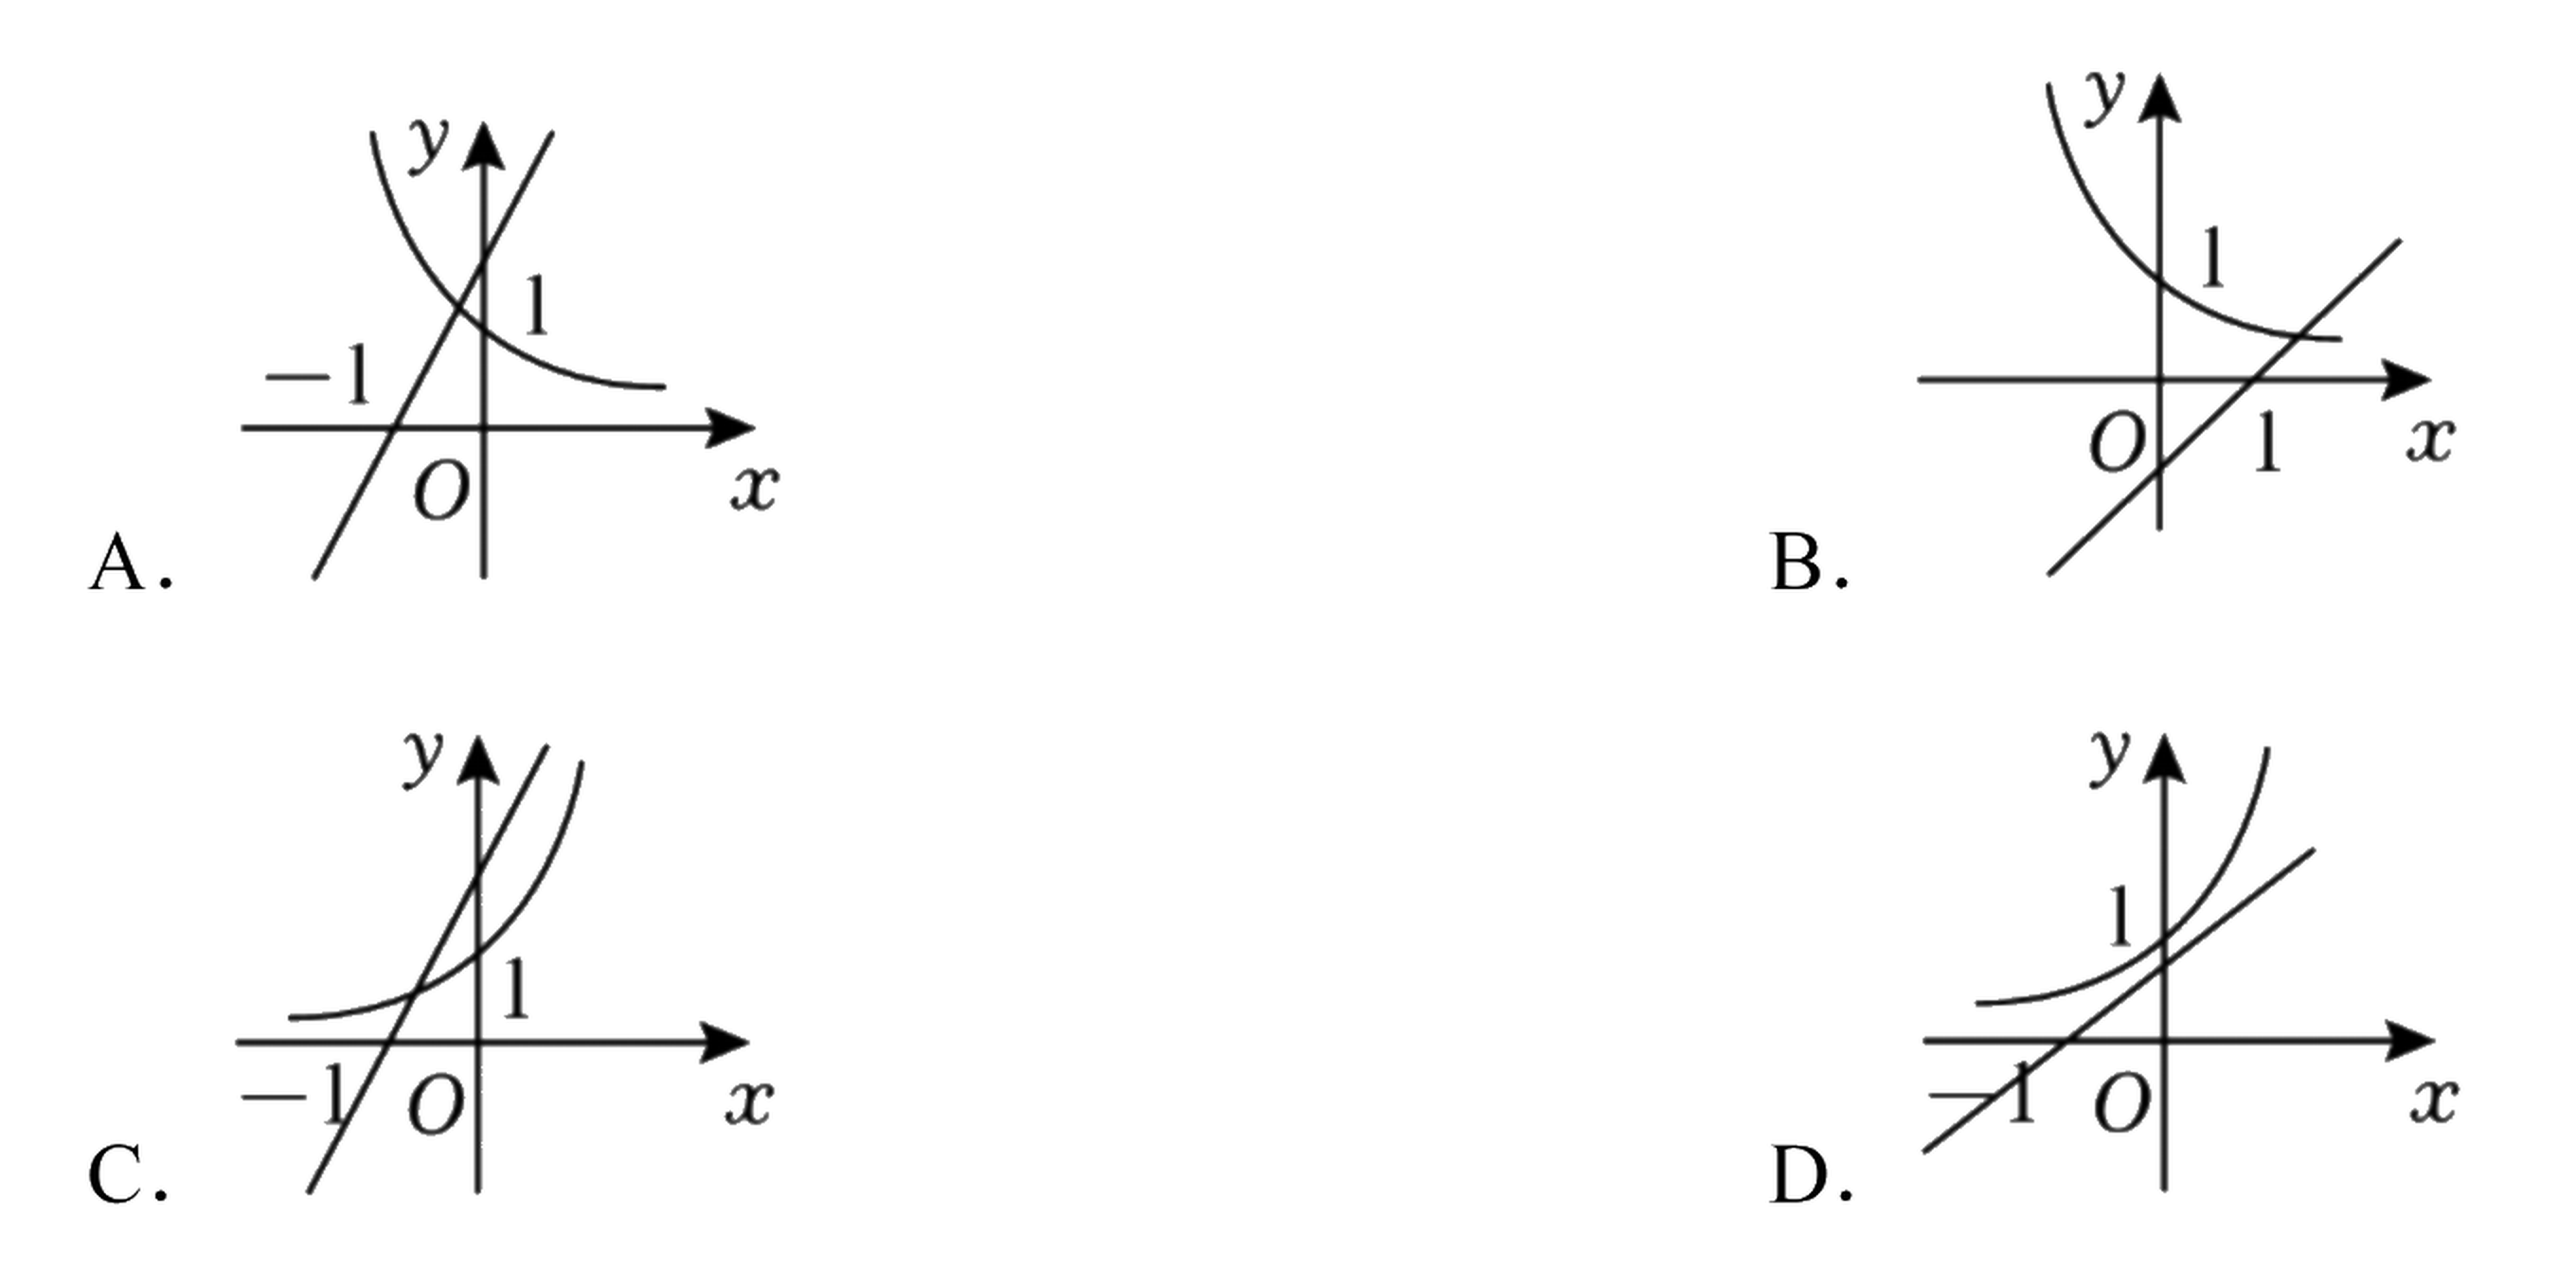
\includegraphics[width=0.80\textwidth]{figures/gao130_q15.png}
\end{center}

\ifanswer
\solbegin
\step{A 中，由指数函数 $y=a^x(a>0$ 且 $a\neq1)$ 图像递减得 $0<a<1$，}
\step{而一次函数 $y=a(x+1)$ 的图像与 $y$ 轴交点纵坐标为 $a>1$，二者矛盾，}
\step{所以 A 错；}
\step{由一次函数 $y=a(x+1)$ 的图像与 $x$ 轴交点横坐标为 $-1$，排除 B；}
\step{C 中，由指数函数 $y=a^x(a>0$ 且 $a\neq1)$ 图像递减得 $a>1$，}% 原卷"递减得 a>1"系笔误（应为"递增"），与 A 中"递减得 0<a<1"自相矛盾，照录
\step{而一次函数 $y=a(x+1)$ 的图像与 $y$ 轴交点纵坐标为 $a>1$，二者 $a$ 值吻合，}
\step{所以 C 对；}
\step{D 中，由一次函数 $y=a(x+1)$ 的图像得 $a=1$，与 $a>0$ 且 $a\neq1$ 矛盾，}
\step{所以 D 错.}
\step{故选 $C$.}
\solend
\fi

\item 设 $A_1$、$A_2$、$A_3$、$\cdots$、$A_7$ 是均含有 $2$ 个元素的集合，且 $A_1\cap A_7=\varnothing$，$A_i\cap A_{i+1}=\varnothing(i=1,2,3,\cdots,6)$，记 $B=A_1\cup A_2\cup A_3\cup\cdots\cup A_7$，则 $B$ 中元素个数的最小值是\mbox{（\quad）}

\keepwithprev
A. $4$\qquad B. $5$\qquad C. $6$\qquad D. $7$

\ifanswer
\solbegin
\step{取 $A_1=\{1,2\}$，$A_2=\{3,4\}$，$A_3=\{1,2\}$，$A_4=\{3,4\}$，$A_5=\{1,5\}$，$A_6=\{2,3\}$，$A_7=\{4,5\}$，}
\step{所以 $B$ 中元素个数的最小值是 $5$，故选 $B$.}
\solend
\fi

\end{enumerate}

\bigsec{三、解答题}

\begin{enumerate}
\setcounter{enumi}{16}

\item 已知全集为 $\R$，集合 $A=\{x\mid-2\leqslant x\leqslant5\}$，集合 $B=\{x\mid m-1\leqslant x\leqslant2m+1\}$．

(1) 求 $\overline{A}$；

(2) 若 $A\cup B=A$，求实数 $m$ 的取值范围．

\ifanswer
\solbegin
\step{(1) $(-\infty,-2)\cup(5,+\infty)$；}
\step{(2) 若 $A\cup B=A$，则 $B\subseteq A$，}
\step{当 $B=\varnothing$ 时，$m-1>2m+1$，解得 $m<-2$；}
\step{当 $B\neq\varnothing$ 时，$\begin{cases}m-1\leqslant2m+1\\m-1\geqslant-2\\2m+1\leqslant5\end{cases}$，解得 $-1\leqslant m\leqslant2$；}
\step{故实数 $m$ 的取值范围为 $\{m\mid-1\leqslant m\leqslant2$ 或 $m<-2\}$.}
\solend
\fi

\item 在不等式的应用中，有一些很基本而十分重要的不等式，如平均值不等式和三角不等式等，我们将其统称为基本不等式．

(1) 已知 $x$、$y$ 为正数，且 $2x+y=2$，求 $\dfrac1x+\dfrac2y$ 的最小值；

(2) 若关于 $x$ 的不等式 $\lvert x+1\rvert+\lvert2-x\rvert\geqslant a^2+a+1$ 对于一切实数 $x$ 都成立，求实数 $a$ 的取值范围．

\ifanswer
\solbegin
\step{(1) 因为 $x$、$y$ 为正数，且 $2x+y=2$，}
\step{所以 $\dfrac1x+\dfrac2y=\dfrac12\left(\dfrac1x+\dfrac2y\right)(2x+y)=\dfrac12\left(4+\dfrac yx+\dfrac{4x}y\right)\geqslant\dfrac12\left(4+2\sqrt{\dfrac yx\cdot\dfrac{4x}y}\right)=4$，}
\step{当且仅当 $\dfrac yx=\dfrac{4x}y$，即 $x=\dfrac12$，$y=1$ 时取等号，所以 $\dfrac1x+\dfrac2y$ 的最小值为 $4$；}
\step{(2) 由绝对值三角不等式得 $\lvert x+1\rvert+\lvert2-x\rvert\geqslant\lvert(x+1)+(2-x)\rvert=3$，}
\step{当且仅当 $-1\leqslant x\leqslant2$ 时取等号，所以 $\lvert x+1\rvert+\lvert2-x\rvert$ 的最小值为 $3$，}
\step{因为关于 $x$ 的不等式 $\lvert x+1\rvert+\lvert2-x\rvert\geqslant a^2+a+1$ 对于一切实数 $x$ 都成立，}
\step{所以 $a^2+a+1\leqslant3$，即 $a^2+a-2\leqslant0$，解得 $-2\leqslant a\leqslant1$，}
\step{所以实数 $a$ 的取值范围是 $[-2,1]$.}
\solend
\fi

\item 某医学专家为研究传染病传播中病毒细胞的发展规律，将病毒细胞注入一只小白鼠体内进行试验，经检测，病毒细胞的个数 $y$ 与天数 $x$ 的部分数据如表所示：

\begin{center}
\begin{tabular}{|c|c|c|c|c|c|c|c|}
\hline
天数 $(x)$ & $1$ & $2$ & $3$ & $4$ & $5$ & $6$ & $\cdots$ \\
\hline
病毒细胞的个数 $(y)$ & $1$ & $2$ & $4$ & $8$ & $16$ & $32$ & $\cdots$ \\
\hline
\end{tabular}
\end{center}

(1) 若病毒细胞的个数 $y$ 关于天数 $x$ 的变化规律可选用以下两个函数模型之一进行近似刻画：① $y=a\cdot b^x(a>0$，$b>0$，$b\neq1)$；② $y=a\cdot x^k(a\neq0)$．请结合表格中的数据，选择合适的函数模型，说明理由，并求出相应的函数表达式；

(2) 若该病毒细胞在小白鼠体内的个数超过 $10^8$，小白鼠将死亡，但注射某种药物，可杀死其体内 $98\%$ 的病毒细胞．则在 (1) 的条件下，为了使小白鼠在试验过程中不死亡，第一次最迟应在何时注射该种药物？（结果精确到天）

\ifanswer
\solbegin
\step{(1) 选择模型① $y=a\cdot b^x(a>0$，$b>0$，$b\neq1)$，理由如下：}
\step{观察表格数据，$y$ 的值随 $x$ 呈指数倍增：}
\step{$x=1$ 时，$y=1$，$x=2$ 时，$y=2$，$x=3$ 时，$y=4$，}
\step{后一天的病毒数是前一天的 $2$ 倍，符合指数增长的特征；}
\step{若选用幂函数模型 $y=a\cdot x^k$，代入前两组数据得 $a\cdot1^k=1$、$a\cdot2^k=2$，}
\step{解得 $a=1$，$k=1$，即 $y=x$，}
\step{但 $x=3$ 时，$y=3$ 与表格中 $y=4$ 严重不符，因此幂函数不匹配；}
\step{将 $(1,1)$ 代入 $y=a\cdot b^x$ 得 $a\cdot b=1$，}
\step{将 $(2,2)$ 代入得 $a\cdot b^2=2$，两式相除得 $b=2$，进而得 $a=\dfrac12$，}
\step{验证所有表格点均满足 $y=2^{x-1}$，最终函数表达式为 $y=2^{x-1}(x\in\N^*)$；}
\step{(2) 由题意得第一次注射药物前病毒细胞个数 $y$ 关于天数 $x(x\in\N^*)$ 的函数}
\step{关系式为 $y=2^{x-1}(x\in\N^*)$，}
\step{为了使小白鼠在试验过程中不死亡，则 $2^{x-1}\leqslant10^8$，}
\step{所以 $x-1\leqslant\log_210^8=8\log_210=\dfrac8{\lg2}$，解得 $x\leqslant1+\dfrac8{\lg2}\approx27.6$，}
\step{又 $x\in\N^*$，所以第一次最迟应在第 $27$ 天注射该种药物.}
\solend
\fi

\item 对在直角坐标系的第一象限内的任意两点 $(a,b)$，$(c,d)$ 作如下定义：$\dfrac ab>\dfrac cd$，那么称点 $(a,b)$ 是点 $(c,d)$ 的“上位点”，同时点 $(c,d)$ 是点 $(a,b)$ 的“下位点”．

(1) 试写出点 $(3,5)$ 的一个“上位点”坐标和一个“下位点”坐标；

(2) 设 $a$、$b$、$c$、$d$ 均为正数，且点 $(a,b)$ 是点 $(c,d)$ 的上位点，请判断点 $P(a+c,b+d)$ 是否既是点 $(a,b)$ 的“下位点”又是点 $(c,d)$ 的“上位点”，如果是，请证明；如果不是，请说明理由；

(3) 设正整数 $n$ 满足以下条件：对任意实数 $m\in\{t\mid0<t<4,t\in\Z\}$，总存在正整数 $k$，使得点 $(n,k)$ 既是点 $(4,m)$ 的“下位点”，又是点 $(5,m+1)$ 的“上位点”，求正整数 $n$ 的最小值．

\ifanswer
\solbegin
\step{(1) 由 $\dfrac34>\dfrac35>\dfrac36$ 得点 $(3,5)$ 的一个“上位点”的坐标为 $(3,4)$，}
\step{一个“下位点”的坐标为 $(3,6)$.}
\step{(2) 是，证明如下：}
\step{因为 $a$、$b$、$c$、$d$ 均为正数，点 $(a,b)$ 是点 $(c,d)$ 的“上位点”，}
\step{所以 $\dfrac ab>\dfrac cd$，所以 $ad>bc$，}
\step{因为 $\dfrac{a+c}{b+d}-\dfrac ab=\dfrac{b(a+c)-a(b+d)}{b(b+d)}=\dfrac{bc-ad}{b(b+d)}<0$，所以 $\dfrac{a+c}{b+d}<\dfrac ab$，}
\step{点 $P(a+c,b+d)$ 是点 $(a,b)$ 的“下位点”，}
\step{因为 $\dfrac{a+c}{b+d}-\dfrac cd=\dfrac{d(a+c)-c(b+d)}{d(b+d)}=\dfrac{ad-bc}{d(b+d)}>0$.}
\step{所以 $\dfrac{a+c}{b+d}>\dfrac cd$ 点 $P(a+c,b+d)$ 是点 $(c,d)$ 的“上位点”；}
\step{所以 $P(a+c,b+d)$ 既是点 $(a,b)$ 的“下位点”又是点 $(c,d)$ 的“上位点”；}
\step{(3) 由题意得 $m=1,2,3$，}
\step{由题意存在正整数 $k$：$\dfrac5{m+1}<\dfrac nk<\dfrac4m$，所以 $\begin{cases}\dfrac n4<k<\dfrac{2n}5(m=1)\\\dfrac n2<k<\dfrac{3n}5(m=2)\\\dfrac{3n}4<k<\dfrac{4n}5(m=3)\end{cases}$，}
\step{检验：$n=1,2,\cdots,8$ 不能同时找到整数 $k$，}
\step{$n=9$：$m=1$ 取 $k=3$，$m=2$ 取 $k=5$，$m=3$ 取 $k=7$，均满足，}
\step{所以正整数 $n$ 的最小值为 $9$.}
\solend
\fi

\end{enumerate}

\end{document}
"
% 紧凑版：xelatex "\def\iscompact{1}% 高一130_北郊高级中学_期中.tex
%   —— 高一上数学"2026-2027 年北郊高级中学高一上期中"（试卷版/答案版）
% 试卷版：xelatex 高一130_北郊高级中学_期中.tex
% 答案版：xelatex "\def\isanswer{1}% 高一130_北郊高级中学_期中.tex
%   —— 高一上数学"2026-2027 年北郊高级中学高一上期中"（试卷版/答案版）
% 试卷版：xelatex 高一130_北郊高级中学_期中.tex
% 答案版：xelatex "\def\isanswer{1}% 高一130_北郊高级中学_期中.tex
%   —— 高一上数学"2026-2027 年北郊高级中学高一上期中"（试卷版/答案版）
% 试卷版：xelatex 高一130_北郊高级中学_期中.tex
% 答案版：xelatex "\def\isanswer{1}\input{高一130_北郊高级中学_期中.tex}"
% 紧凑版：xelatex "\def\iscompact{1}\input{高一130_北郊高级中学_期中.tex}"
%
% ① 原始材料：微信公众号"魔都数学加油站"文章，连载"27学年高一140"，原文标题
% "27学年高一140——2026-2027年上海市北郊高级中学高一上期中"；
% 原文链接：https://mp.weixin.qq.com/s/XBEYuTheiBoqu15dtLuD6A。
%   ★ 编号不一致说明：公众号连载号印"140"，与上一批已入库的"高一140 甘泉外国语"
%   （同一公众号另一篇文章、同为期中卷）撞号，系公众号笔误/重复。本仓库数字编号
%   02—143 中"高一130"一直空缺（连载 130 暂未见原文），故将本卷本地编号定为"高一130"、
%   填补该空缺，使数字编号连续（basename 全程为 高一130_北郊高级中学_期中）；
%   连载号 143 归正牌卷"上海中学 高一上期中"；本卷连载号仍印 140，见材料流转表。
%   卷面标题印"2026-2027 年北郊高级中学高一上期中"（卷面只有学校名、不含"上海市"、
%   不含任何期号/连载号），本稿照卷面录入；粉红色水印"魔都数学加油站"及页脚未录入。
% 正文为 9 张 PNG 页（01、04、05、06、09 为 2560x3620；02、03、07、08 为 4762x6735，
% 同一篇各页分辨率不同，逐页按各自分辨率放大核对），题目下印有【解析】，为讲评版。
% 题目、解析均据原图转录。
%
% 卷首标题：原卷印作"2026-2027 年北郊高级中学高一上期中"，年份区间按全稿惯例排
% en dash；原卷未印副标题，本卷为期中卷、跨集合与常用逻辑用语／不等式／函数三章，
% 按题目内容补出"集合与常用逻辑用语、不等式、函数"（与 125／126／128／129／131／132／133
% 同期中卷口径相同）。
%
% 题号体例：本卷共 18 题——一、填空题 3—12（10 题）、二、选择题 13—16（4 题）、
% 三、解答题 17—20（4 题）。三节分别 \setcounter{enumi}{2}／{12}／{16}。
% 原卷从第 3 题起、无第 1、2 题、**无第 21 题**（第 20 题解析续至 09 页，末行
% "所以正整数 n 的最小值为 9."，09 页下半页整片空白＋水印收尾、无第 10 页），本稿保留原题号。
%
% ② 与原卷的排版差异：
%   ① 原文从第 3 题起，本稿保留原题号；原卷止于第 20 题、无第 21 题、无附加题节；
%   ② 原卷每题下直接印【解析】，本稿按全稿惯例置于答案版；全卷 18 题均印【解析】、
%      无独立【答案】段，四道选择题答案在解析末句"故选 C／D／C／B"，括号
%      \mbox{（\quad）} 留空、不另提 \ans{}；全卷 0 处 \ans{}，答案版【解析】标记数 18＝题数；
%   ③ 原卷未印副标题，本稿按"知识模块"口径补出；
%   ④ 原卷填空横线按全稿惯例排为 \blankline[4.4em]；选择题括号排 \mbox{（\quad）}、
%      每个选项段前按惯例加 \keepwithprev；解答题不留作答区、不加 \anspace（讲评版）；
%   ⑤ 原卷数集排斜体 $R$／$N$，按全稿惯例改 \R／\N；空集记号 \varnothing；
%      绝对值排 \lvert…\rvert，集合描述竖线排 \mid；不等号按全稿惯例排 \leqslant／\geqslant；
%      补集照原卷上划线 \overline{A}；
%   ⑥ 1 幅插图 + 1 张印刷表格：第 15 题四幅坐标函数图象选项（04 页）取原卷截图
%      去粉色水印、去色、按原卷 2x2 排布合并为 figures/gao130_q15.png（非插图重绘），
%      放在 \keepwithprev 之后 \begin{center} 内、三版都出；第 19 题 (1) 印刷数据表格
%      （07 页，天数 x 1—6／病毒细胞个数 y 1/2/4/8/16/32）按原卷用 tabular 重排、
%      题干内三版都出（非插图）。
%      第 15 题是"二、选择题"节内带大图块的第三题（Q13 为节首题但无图），
%      在 \bigsec{二、选择题} 之前加 \needvspace{11cm} 连节标题一起量、Q15 \item 之前
%      加 \needvspace{9cm}——守卫必须放在 \bigsec 之前，放标题之后会让"二、选择题"
%      孤立在页末（B 类，照 高一26／40／59／136／140 成例）；三版切页审计均"合计异常：无"；
%   ⑦ 子题标号 (1)(2)(3) 原卷用半角括号，照录；圈数字 ①②③④ 照录；
%      数学式内半角逗号照录（如第 14 题 $(a>0,a\neq1)$、第 16 题
%      $(i=1,2,3,\cdots,6)$、第 20 题 $m=1,2,3$ 等）；
%      行末西文句点按全稿惯例照录；
%   ⑧ 题干中的中文弯引号按原卷照录（Q12"变项和"、Q20"上位点""下位点"等），
%      注释内一律 ASCII 引号；原卷"图像"用词逐处照录（Q9、Q15 均作"图像"）。
%
% ③ 行数复核：一条 \step = 原卷解析的一个印刷行（cases 块与 tabular 各作一个印刷行计）。
%   逐题 \step 条数，合计 98 条（Q3:3 Q4:2 Q5:2 Q6:1 Q7:1 Q8:3 Q9:5 Q10:10 Q11:6
%   Q12:7 Q13:1 Q14:2 Q15:10 Q16:2 Q17:5 Q18:8 Q19:15 Q20:15），与原卷印刷行逐题相等。
%
% ④ 判别式／子集符号结论：
%   判别式：全卷未出现判别式记号（无 $\Delta$、无 $\triangle$）；
%   子集符号：第 4 题题干"$B\subseteq A$"、第 4 题【解析】"$B\subseteq A$"、
%      第 17 题 (2)【解析】"$B\subseteq A$"三处原卷均印带下划线 $\subseteq$，逐处
%      放大核对、照录 \subseteq；全卷未出现单线 \subset。
%
% ⑤ 原卷存疑照录（均照录未改，正文对应处另有 % 注）：
%   ① 第 15 题【解析】"C 中，由指数函数 $y=a^x$ 图像递减得 $a>1$"——"递减"应为
%      "递增"之误（与同题 A 中"递减得 $0<a<1$"自相矛盾），原卷如此，照录并加注；
%   ② 第 16 题题干"$A_1\cap A_7=\varnothing$""$A_i\cap A_{i+1}=\varnothing$"
%      的空集记号与解析所列各集合逐处照录；
%   ③ 第 19 题 (2) 题干"可杀死其体内 98% 的病毒细胞"、解析 (2) 只按 $y=2^{x-1}$
%      与 $10^8$ 比较（未另计 98%），照录不补步。
%
% ⑥ 跨页续印按题合并：Q8 题干在 01 页末、解析在 02 页；Q9 题干在 02 页、
%   解析在 02 页；Q10 题干在 02 页、解析前 5 行在 02—03 页、后 5 行在 03 页；
%   Q12 题干跨 03 页、解析首 5 行在 03 页末、末行在 04 页；Q15 题干在 04 页、
%   四幅图与解析前段在 04 页、解析续在 05 页；Q17 解析跨 05—06 页；Q18 题干与
%   (1) 解析在 06 页、(2) 解析在 06—07 页；Q19 表格在 07 页、解析跨 07—08 页；
%   Q20 定义与三小问在 08 页、解析 (1)(2) 在 08—09 页、解析 (3) 在 09 页；
%   本稿按题连排，不丢行。
%
\documentclass[a4paper,11pt]{article}
\usepackage{common}

\begin{document}

\examtitlest[3]{2026--2027 年北郊高级中学高一上期中}{集合与常用逻辑用语、不等式、函数}

\bigsec{一、填空题}

\begin{enumerate}
\setcounter{enumi}{2}

\item 不等式 $\dfrac{x-3}{x+1}<2$ 的解集为\blankline[4.4em].

\ifanswer
\solbegin
\step{不等式 $\dfrac{x-3}{x+1}<2$ 可化为 $\dfrac{x-3}{x+1}-2<0$，即 $\dfrac{x-3-2(x+1)}{x+1}<0$，}
\step{化简为 $\dfrac{x+5}{x+1}>0$，解得 $x<-5$ 或 $x>-1$，}
\step{所以不等式的解集为 $\{x\mid x<-5$ 或 $x>-1\}$.}
\solend
\fi

\item 已知集合 $A=\{x\mid0<x<a\}$，$B=\{x\mid1<x<2\}$，若 $B\subseteq A$，则实数 $a$ 的取值范围为\blankline[4.4em].

\ifanswer
\solbegin
\step{已知集合 $A=\{x\mid0<x<a\}$，$B=\{x\mid1<x<2\}$，}
\step{若 $B\subseteq A$，则 $a\geqslant2$，所以实数 $a$ 的取值范围是 $\{a\mid a\geqslant2\}$.}
\solend
\fi

\item 已知关于 $x$ 的方程 $x^2+x+c=0$ 的两个实数根为 $x_1$、$x_2$，若 $x_1^2x_2+x_2^2x_1=3$，则实数 $c=$\blankline[4.4em].

\ifanswer
\solbegin
\step{由韦达定理得 $x_1+x_2=-1$，$x_1x_2=c$，所以 $x_1^2x_2+x_2^2x_1=(x_1+x_2)x_1x_2=-c=3$，}
\step{所以 $c=-3$.}
\solend
\fi

\item 已知 $10^x=3$，$10^y=64$，则 $10^{x-\frac y3}=$\blankline[4.4em].

\ifanswer
\solbegin
\step{$10^{x-\frac y3}=10^x\div\sqrt[3]{10^y}=\dfrac34$.}
\solend
\fi

\item 若 $\lg2=a$，则可用 $a$ 表示 $\log_280=$\blankline[4.4em].

\ifanswer
\solbegin
\step{$\log_280=\dfrac{\lg80}{\lg2}=\dfrac{\lg10+\lg8}{\lg2}=\dfrac{1+3\lg2}{\lg2}=\dfrac{1+3a}{a}$.}
\solend
\fi

\item 已知 $a+2b=1$，则 $3^a+9^b$ 的最小值为\blankline[4.4em].

\ifanswer
\solbegin
\step{因为 $a+2b=1$，所以 $3^a+9^b=3^a+3^{2b}\geqslant2\sqrt{3^a\cdot3^{2b}}=2\sqrt{3^{a+2b}}=2\sqrt3$，}
\step{当且仅当 $3^a=3^{2b}$，且 $a+2b=1$，即 $a=\dfrac12$，$b=\dfrac14$ 时取等号，}
\step{故最小值为 $2\sqrt3$.}
\solend
\fi

\item 下列函数的图像关于原点成中心对称，且在区间 $(0,+\infty)$ 上是严格增函数的是\blankline[4.4em]（请填写全部正确的序号）.

① $y=\sqrt{x}$；② $y=\sqrt[3]{x}$；③ $y=x^{\frac23}$；④ $y=x^{-\frac13}$.

\ifanswer
\solbegin
\step{① $y=\sqrt{x}$ 的定义域为 $[0,+\infty)$，故其图像不关于原点成中心对称，①错误；}
\step{② $y=\sqrt[3]{x}$ 是奇函数，且在区间 $(0,+\infty)$ 上是严格增函数，②正确；}
\step{③ $y=x^{\frac23}$ 是偶函数，其图像关于 $y$ 轴对称，不关于原点成中心对称，③错误；}
\step{④由于幂指数 $-\dfrac13<0$，故 $y=x^{-\frac13}$ 在区间 $(0,+\infty)$ 上是严格减函数，④错误.}
\step{故正确的是②.}
\solend
\fi

\item 设 $a>0$ 且 $a\neq1$，若函数 $y=a^{2x}+2a^x-3$ 在区间 $[-1,1]$ 上的最大值为 $21$，则实数 $a$ 的值为\blankline[4.4em].

\ifanswer
\solbegin
\step{令 $t=a^x$，$x\in[-1,1]$，}
\step{当 $a>1$ 时，$t=a^x$ 严格增，则 $t\in\left[\dfrac1a,a\right]$，}
\step{则函数 $y=t^2+2t-3$，对称轴为 $t=-1$，}
\step{所以函数 $y=t^2+2t-3$ 在 $\left[\dfrac1a,a\right]$ 上严格增，}
\step{所以当 $t=a$ 时，$y$ 取得最大值 $a^2+2a-3=21$，解得 $a=4$ 或 $-6$（舍去）；}
\step{当 $0<a<1$ 时，$t=a^x$ 严格减，则 $t\in\left[a,\dfrac1a\right]$，}
\step{则函数 $y=t^2+2t-3$，对称轴为 $t=-1$，}
\step{所以函数 $y=t^2+2t-3$ 在 $\left[a,\dfrac1a\right]$ 上严格增，}
\step{所以当 $t=\dfrac1a$ 时，$y$ 取得最大值 $\dfrac1{a^2}+\dfrac2a-3=21$，解得 $a=\dfrac14$ 或 $-\dfrac16$（舍去）；}
\step{综上所述，实数 $a$ 的值为 $4$ 或 $\dfrac14$.}
\solend
\fi

\item 在关于 $x$ 的不等式 $x^2+(m+1)x+m<0$ 的解集中恰有两个整数，则实数 $m$ 的取值范围是\blankline[4.4em].

\ifanswer
\solbegin
\step{关于 $x$ 的不等式 $x^2+(m+1)x+m<0$ 可化为 $(x+1)(x+m)<0$，}
\step{当 $m>1$ 时，$-m<-1$，解不等式得 $-m<x<-1$；}
\step{当 $m<1$ 时，$-m>-1$，解不等式得 $-1<x<-m$；}
\step{由不等式的解集中恰有两个整数，}
\step{则 $-4\leqslant-m<-3$ 或 $1<-m\leqslant2$，即 $3<m\leqslant4$ 或 $-2\leqslant m<-1$，}
\step{所以 $m$ 的取值范围是 $[-2,-1)\cup(3,4]$.}
\solend
\fi

\item 已知集合 $M$ 的元素均为正整数，定义集合 $M$ 的“变项和”为：将 $M$ 中每个元素 $m$ 都乘以 $(-1)^m$ 后再求和．若集合 $A=\{n\mid1\leqslant n\leqslant20,n\in\N\}$，则集合 $A$ 的所有非空子集的“变项和”的总和为\blankline[4.4em].

\ifanswer
\solbegin
\step{集合 $A=\{n\mid1\leqslant n\leqslant20,n\in\N\}$ 中一共有 $20$ 个元素，}
\step{固定选中 $k$，剩下 $19$ 个元素任选，共 $2^{19}$ 个子集包含 $k$，每个 $k$ 贡献 $(-1)^k\cdot k\cdot2^{19}$，}
\step{$A=\{1,2,\cdots,20\}$，}
\step{奇数 $k=1,3,\cdots,19$，共 $10$ 个，$(-1)^k\cdot k=-k$，}
\step{偶数 $k=2,4,\cdots,20$，共 $10$ 个，$(-1)^k\cdot k=k$，}
\step{所以集合 $A$ 的所有非空子集的“变项和”的总和}
\step{为 $S=2^{19}\times[(-1+2)+(-3+4)+\cdots+(-19+20)]=2^{19}\times10=524880$.}
\solend
\fi

\end{enumerate}

% 第 15 题四幅图是"二、选择题"节内大图块；守卫须放在 \bigsec 之前连节标题一起量，
% 否则"二、选择题"会孤立在页末（B 类，照 高一26／40／59／136／140 成例）
\needvspace{11cm}
\bigsec{二、选择题}

\begin{enumerate}
\setcounter{enumi}{12}

\item 设 $ab>0$，则“$a>b$”是“$\dfrac1a<\dfrac1b$”的\mbox{（\quad）}

\keepwithprev
A. 充分非必要条件\qquad B. 必要非充分条件

C. 充要条件\qquad D. 既非充分也非必要条件

\ifanswer
\solbegin
\step{因为 $ab>0$，所以 $a>b\Leftrightarrow\dfrac1a<\dfrac1b$，故选 $C$.}
\solend
\fi

\item 已知 $A=\log_ax$，$B=\log_ay(a>0,a\neq1)$，则 $\log_a\dfrac{x^2}{\sqrt y}=$\mbox{（\quad）}

\keepwithprev
A. $\dfrac{A^2}{\sqrt B}$\qquad B. $2A^2B$\qquad C. $4AB$\qquad D. $2A-\dfrac12B$

\ifanswer
\solbegin
\step{由已知得 $x=a^A$，$y=a^B$，}
\step{所以 $\log_a\dfrac{x^2}{\sqrt y}=\log_a\dfrac{(a^A)^2}{\sqrt{a^B}}=\log_a\dfrac{a^{2A}}{a^{\frac12B}}=\log_a a^{2A-\frac12B}=2A-\dfrac12B$. 故选 $D$.}
\solend
\fi

% 第 15 题四幅坐标函数图象选项是一整块，守卫放在 \item 之前
\needvspace{9cm}
\item 在同一平面直角坐标系中，指数函数 $y=a^x(a>0$ 且 $a\neq1)$ 和一次函数 $y=a(x+1)$ 的图像关系可能是\mbox{（\quad）}

\keepwithprev
\begin{center}
% 四幅坐标函数图象选项取原卷 04 页截图去粉色水印、去色，按原卷 2x2 排布合并为一张
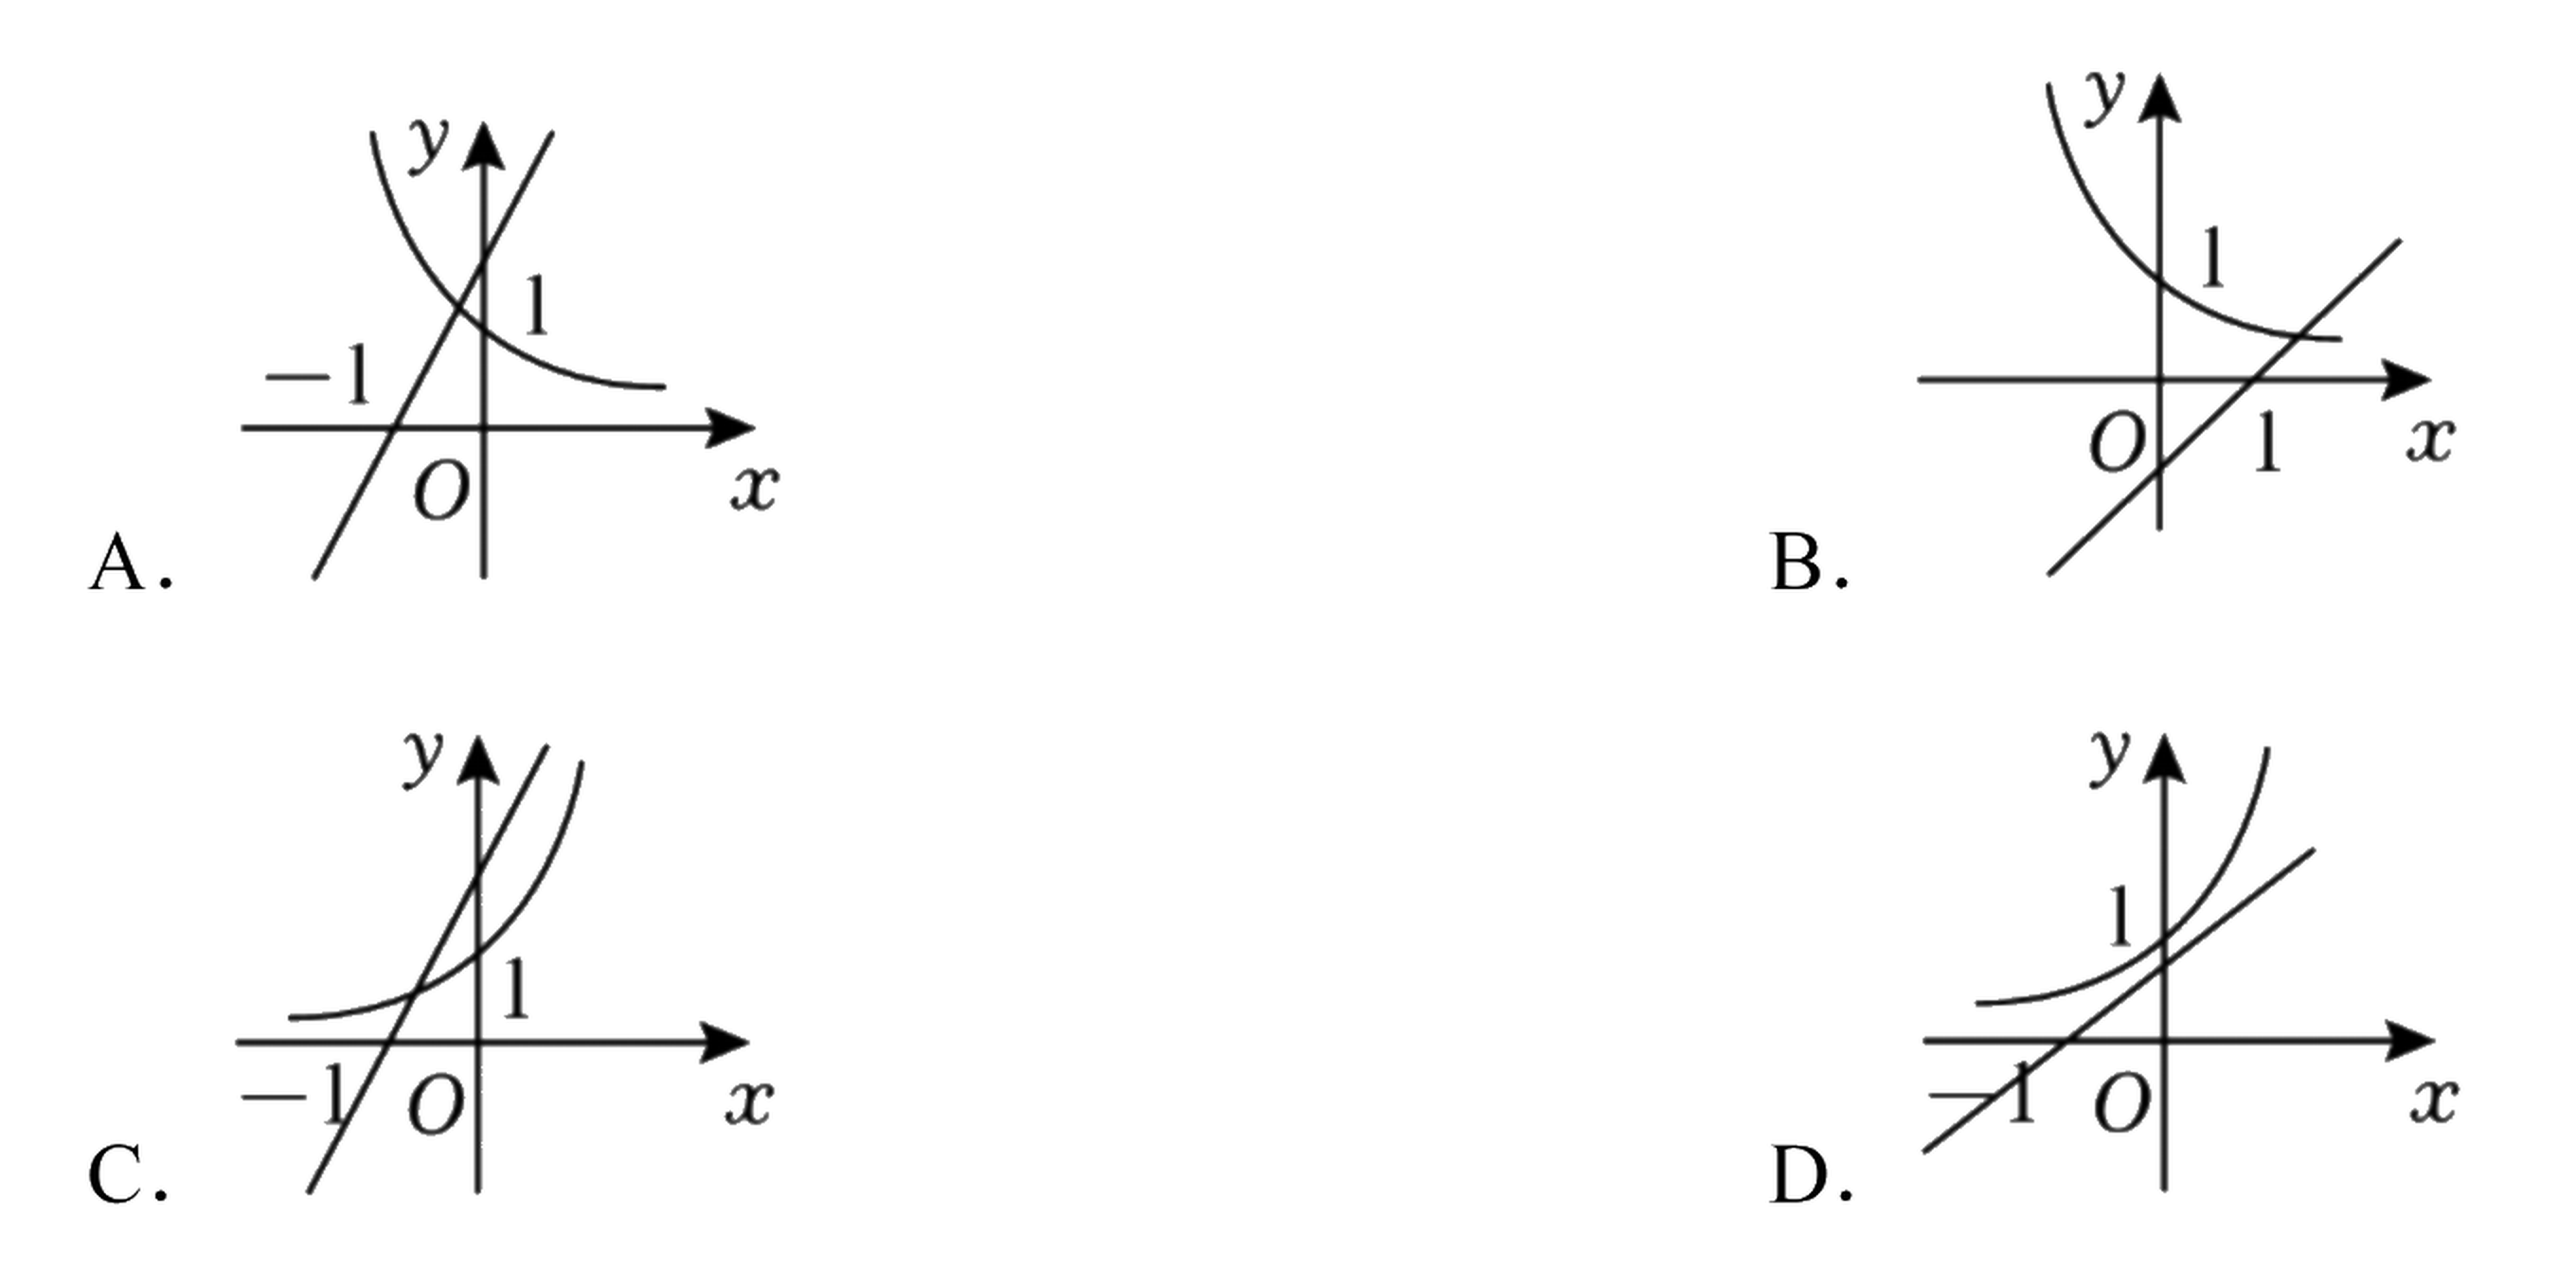
\includegraphics[width=0.80\textwidth]{figures/gao130_q15.png}
\end{center}

\ifanswer
\solbegin
\step{A 中，由指数函数 $y=a^x(a>0$ 且 $a\neq1)$ 图像递减得 $0<a<1$，}
\step{而一次函数 $y=a(x+1)$ 的图像与 $y$ 轴交点纵坐标为 $a>1$，二者矛盾，}
\step{所以 A 错；}
\step{由一次函数 $y=a(x+1)$ 的图像与 $x$ 轴交点横坐标为 $-1$，排除 B；}
\step{C 中，由指数函数 $y=a^x(a>0$ 且 $a\neq1)$ 图像递减得 $a>1$，}% 原卷"递减得 a>1"系笔误（应为"递增"），与 A 中"递减得 0<a<1"自相矛盾，照录
\step{而一次函数 $y=a(x+1)$ 的图像与 $y$ 轴交点纵坐标为 $a>1$，二者 $a$ 值吻合，}
\step{所以 C 对；}
\step{D 中，由一次函数 $y=a(x+1)$ 的图像得 $a=1$，与 $a>0$ 且 $a\neq1$ 矛盾，}
\step{所以 D 错.}
\step{故选 $C$.}
\solend
\fi

\item 设 $A_1$、$A_2$、$A_3$、$\cdots$、$A_7$ 是均含有 $2$ 个元素的集合，且 $A_1\cap A_7=\varnothing$，$A_i\cap A_{i+1}=\varnothing(i=1,2,3,\cdots,6)$，记 $B=A_1\cup A_2\cup A_3\cup\cdots\cup A_7$，则 $B$ 中元素个数的最小值是\mbox{（\quad）}

\keepwithprev
A. $4$\qquad B. $5$\qquad C. $6$\qquad D. $7$

\ifanswer
\solbegin
\step{取 $A_1=\{1,2\}$，$A_2=\{3,4\}$，$A_3=\{1,2\}$，$A_4=\{3,4\}$，$A_5=\{1,5\}$，$A_6=\{2,3\}$，$A_7=\{4,5\}$，}
\step{所以 $B$ 中元素个数的最小值是 $5$，故选 $B$.}
\solend
\fi

\end{enumerate}

\bigsec{三、解答题}

\begin{enumerate}
\setcounter{enumi}{16}

\item 已知全集为 $\R$，集合 $A=\{x\mid-2\leqslant x\leqslant5\}$，集合 $B=\{x\mid m-1\leqslant x\leqslant2m+1\}$．

(1) 求 $\overline{A}$；

(2) 若 $A\cup B=A$，求实数 $m$ 的取值范围．

\ifanswer
\solbegin
\step{(1) $(-\infty,-2)\cup(5,+\infty)$；}
\step{(2) 若 $A\cup B=A$，则 $B\subseteq A$，}
\step{当 $B=\varnothing$ 时，$m-1>2m+1$，解得 $m<-2$；}
\step{当 $B\neq\varnothing$ 时，$\begin{cases}m-1\leqslant2m+1\\m-1\geqslant-2\\2m+1\leqslant5\end{cases}$，解得 $-1\leqslant m\leqslant2$；}
\step{故实数 $m$ 的取值范围为 $\{m\mid-1\leqslant m\leqslant2$ 或 $m<-2\}$.}
\solend
\fi

\item 在不等式的应用中，有一些很基本而十分重要的不等式，如平均值不等式和三角不等式等，我们将其统称为基本不等式．

(1) 已知 $x$、$y$ 为正数，且 $2x+y=2$，求 $\dfrac1x+\dfrac2y$ 的最小值；

(2) 若关于 $x$ 的不等式 $\lvert x+1\rvert+\lvert2-x\rvert\geqslant a^2+a+1$ 对于一切实数 $x$ 都成立，求实数 $a$ 的取值范围．

\ifanswer
\solbegin
\step{(1) 因为 $x$、$y$ 为正数，且 $2x+y=2$，}
\step{所以 $\dfrac1x+\dfrac2y=\dfrac12\left(\dfrac1x+\dfrac2y\right)(2x+y)=\dfrac12\left(4+\dfrac yx+\dfrac{4x}y\right)\geqslant\dfrac12\left(4+2\sqrt{\dfrac yx\cdot\dfrac{4x}y}\right)=4$，}
\step{当且仅当 $\dfrac yx=\dfrac{4x}y$，即 $x=\dfrac12$，$y=1$ 时取等号，所以 $\dfrac1x+\dfrac2y$ 的最小值为 $4$；}
\step{(2) 由绝对值三角不等式得 $\lvert x+1\rvert+\lvert2-x\rvert\geqslant\lvert(x+1)+(2-x)\rvert=3$，}
\step{当且仅当 $-1\leqslant x\leqslant2$ 时取等号，所以 $\lvert x+1\rvert+\lvert2-x\rvert$ 的最小值为 $3$，}
\step{因为关于 $x$ 的不等式 $\lvert x+1\rvert+\lvert2-x\rvert\geqslant a^2+a+1$ 对于一切实数 $x$ 都成立，}
\step{所以 $a^2+a+1\leqslant3$，即 $a^2+a-2\leqslant0$，解得 $-2\leqslant a\leqslant1$，}
\step{所以实数 $a$ 的取值范围是 $[-2,1]$.}
\solend
\fi

\item 某医学专家为研究传染病传播中病毒细胞的发展规律，将病毒细胞注入一只小白鼠体内进行试验，经检测，病毒细胞的个数 $y$ 与天数 $x$ 的部分数据如表所示：

\begin{center}
\begin{tabular}{|c|c|c|c|c|c|c|c|}
\hline
天数 $(x)$ & $1$ & $2$ & $3$ & $4$ & $5$ & $6$ & $\cdots$ \\
\hline
病毒细胞的个数 $(y)$ & $1$ & $2$ & $4$ & $8$ & $16$ & $32$ & $\cdots$ \\
\hline
\end{tabular}
\end{center}

(1) 若病毒细胞的个数 $y$ 关于天数 $x$ 的变化规律可选用以下两个函数模型之一进行近似刻画：① $y=a\cdot b^x(a>0$，$b>0$，$b\neq1)$；② $y=a\cdot x^k(a\neq0)$．请结合表格中的数据，选择合适的函数模型，说明理由，并求出相应的函数表达式；

(2) 若该病毒细胞在小白鼠体内的个数超过 $10^8$，小白鼠将死亡，但注射某种药物，可杀死其体内 $98\%$ 的病毒细胞．则在 (1) 的条件下，为了使小白鼠在试验过程中不死亡，第一次最迟应在何时注射该种药物？（结果精确到天）

\ifanswer
\solbegin
\step{(1) 选择模型① $y=a\cdot b^x(a>0$，$b>0$，$b\neq1)$，理由如下：}
\step{观察表格数据，$y$ 的值随 $x$ 呈指数倍增：}
\step{$x=1$ 时，$y=1$，$x=2$ 时，$y=2$，$x=3$ 时，$y=4$，}
\step{后一天的病毒数是前一天的 $2$ 倍，符合指数增长的特征；}
\step{若选用幂函数模型 $y=a\cdot x^k$，代入前两组数据得 $a\cdot1^k=1$、$a\cdot2^k=2$，}
\step{解得 $a=1$，$k=1$，即 $y=x$，}
\step{但 $x=3$ 时，$y=3$ 与表格中 $y=4$ 严重不符，因此幂函数不匹配；}
\step{将 $(1,1)$ 代入 $y=a\cdot b^x$ 得 $a\cdot b=1$，}
\step{将 $(2,2)$ 代入得 $a\cdot b^2=2$，两式相除得 $b=2$，进而得 $a=\dfrac12$，}
\step{验证所有表格点均满足 $y=2^{x-1}$，最终函数表达式为 $y=2^{x-1}(x\in\N^*)$；}
\step{(2) 由题意得第一次注射药物前病毒细胞个数 $y$ 关于天数 $x(x\in\N^*)$ 的函数}
\step{关系式为 $y=2^{x-1}(x\in\N^*)$，}
\step{为了使小白鼠在试验过程中不死亡，则 $2^{x-1}\leqslant10^8$，}
\step{所以 $x-1\leqslant\log_210^8=8\log_210=\dfrac8{\lg2}$，解得 $x\leqslant1+\dfrac8{\lg2}\approx27.6$，}
\step{又 $x\in\N^*$，所以第一次最迟应在第 $27$ 天注射该种药物.}
\solend
\fi

\item 对在直角坐标系的第一象限内的任意两点 $(a,b)$，$(c,d)$ 作如下定义：$\dfrac ab>\dfrac cd$，那么称点 $(a,b)$ 是点 $(c,d)$ 的“上位点”，同时点 $(c,d)$ 是点 $(a,b)$ 的“下位点”．

(1) 试写出点 $(3,5)$ 的一个“上位点”坐标和一个“下位点”坐标；

(2) 设 $a$、$b$、$c$、$d$ 均为正数，且点 $(a,b)$ 是点 $(c,d)$ 的上位点，请判断点 $P(a+c,b+d)$ 是否既是点 $(a,b)$ 的“下位点”又是点 $(c,d)$ 的“上位点”，如果是，请证明；如果不是，请说明理由；

(3) 设正整数 $n$ 满足以下条件：对任意实数 $m\in\{t\mid0<t<4,t\in\Z\}$，总存在正整数 $k$，使得点 $(n,k)$ 既是点 $(4,m)$ 的“下位点”，又是点 $(5,m+1)$ 的“上位点”，求正整数 $n$ 的最小值．

\ifanswer
\solbegin
\step{(1) 由 $\dfrac34>\dfrac35>\dfrac36$ 得点 $(3,5)$ 的一个“上位点”的坐标为 $(3,4)$，}
\step{一个“下位点”的坐标为 $(3,6)$.}
\step{(2) 是，证明如下：}
\step{因为 $a$、$b$、$c$、$d$ 均为正数，点 $(a,b)$ 是点 $(c,d)$ 的“上位点”，}
\step{所以 $\dfrac ab>\dfrac cd$，所以 $ad>bc$，}
\step{因为 $\dfrac{a+c}{b+d}-\dfrac ab=\dfrac{b(a+c)-a(b+d)}{b(b+d)}=\dfrac{bc-ad}{b(b+d)}<0$，所以 $\dfrac{a+c}{b+d}<\dfrac ab$，}
\step{点 $P(a+c,b+d)$ 是点 $(a,b)$ 的“下位点”，}
\step{因为 $\dfrac{a+c}{b+d}-\dfrac cd=\dfrac{d(a+c)-c(b+d)}{d(b+d)}=\dfrac{ad-bc}{d(b+d)}>0$.}
\step{所以 $\dfrac{a+c}{b+d}>\dfrac cd$ 点 $P(a+c,b+d)$ 是点 $(c,d)$ 的“上位点”；}
\step{所以 $P(a+c,b+d)$ 既是点 $(a,b)$ 的“下位点”又是点 $(c,d)$ 的“上位点”；}
\step{(3) 由题意得 $m=1,2,3$，}
\step{由题意存在正整数 $k$：$\dfrac5{m+1}<\dfrac nk<\dfrac4m$，所以 $\begin{cases}\dfrac n4<k<\dfrac{2n}5(m=1)\\\dfrac n2<k<\dfrac{3n}5(m=2)\\\dfrac{3n}4<k<\dfrac{4n}5(m=3)\end{cases}$，}
\step{检验：$n=1,2,\cdots,8$ 不能同时找到整数 $k$，}
\step{$n=9$：$m=1$ 取 $k=3$，$m=2$ 取 $k=5$，$m=3$ 取 $k=7$，均满足，}
\step{所以正整数 $n$ 的最小值为 $9$.}
\solend
\fi

\end{enumerate}

\end{document}
"
% 紧凑版：xelatex "\def\iscompact{1}% 高一130_北郊高级中学_期中.tex
%   —— 高一上数学"2026-2027 年北郊高级中学高一上期中"（试卷版/答案版）
% 试卷版：xelatex 高一130_北郊高级中学_期中.tex
% 答案版：xelatex "\def\isanswer{1}\input{高一130_北郊高级中学_期中.tex}"
% 紧凑版：xelatex "\def\iscompact{1}\input{高一130_北郊高级中学_期中.tex}"
%
% ① 原始材料：微信公众号"魔都数学加油站"文章，连载"27学年高一140"，原文标题
% "27学年高一140——2026-2027年上海市北郊高级中学高一上期中"；
% 原文链接：https://mp.weixin.qq.com/s/XBEYuTheiBoqu15dtLuD6A。
%   ★ 编号不一致说明：公众号连载号印"140"，与上一批已入库的"高一140 甘泉外国语"
%   （同一公众号另一篇文章、同为期中卷）撞号，系公众号笔误/重复。本仓库数字编号
%   02—143 中"高一130"一直空缺（连载 130 暂未见原文），故将本卷本地编号定为"高一130"、
%   填补该空缺，使数字编号连续（basename 全程为 高一130_北郊高级中学_期中）；
%   连载号 143 归正牌卷"上海中学 高一上期中"；本卷连载号仍印 140，见材料流转表。
%   卷面标题印"2026-2027 年北郊高级中学高一上期中"（卷面只有学校名、不含"上海市"、
%   不含任何期号/连载号），本稿照卷面录入；粉红色水印"魔都数学加油站"及页脚未录入。
% 正文为 9 张 PNG 页（01、04、05、06、09 为 2560x3620；02、03、07、08 为 4762x6735，
% 同一篇各页分辨率不同，逐页按各自分辨率放大核对），题目下印有【解析】，为讲评版。
% 题目、解析均据原图转录。
%
% 卷首标题：原卷印作"2026-2027 年北郊高级中学高一上期中"，年份区间按全稿惯例排
% en dash；原卷未印副标题，本卷为期中卷、跨集合与常用逻辑用语／不等式／函数三章，
% 按题目内容补出"集合与常用逻辑用语、不等式、函数"（与 125／126／128／129／131／132／133
% 同期中卷口径相同）。
%
% 题号体例：本卷共 18 题——一、填空题 3—12（10 题）、二、选择题 13—16（4 题）、
% 三、解答题 17—20（4 题）。三节分别 \setcounter{enumi}{2}／{12}／{16}。
% 原卷从第 3 题起、无第 1、2 题、**无第 21 题**（第 20 题解析续至 09 页，末行
% "所以正整数 n 的最小值为 9."，09 页下半页整片空白＋水印收尾、无第 10 页），本稿保留原题号。
%
% ② 与原卷的排版差异：
%   ① 原文从第 3 题起，本稿保留原题号；原卷止于第 20 题、无第 21 题、无附加题节；
%   ② 原卷每题下直接印【解析】，本稿按全稿惯例置于答案版；全卷 18 题均印【解析】、
%      无独立【答案】段，四道选择题答案在解析末句"故选 C／D／C／B"，括号
%      \mbox{（\quad）} 留空、不另提 \ans{}；全卷 0 处 \ans{}，答案版【解析】标记数 18＝题数；
%   ③ 原卷未印副标题，本稿按"知识模块"口径补出；
%   ④ 原卷填空横线按全稿惯例排为 \blankline[4.4em]；选择题括号排 \mbox{（\quad）}、
%      每个选项段前按惯例加 \keepwithprev；解答题不留作答区、不加 \anspace（讲评版）；
%   ⑤ 原卷数集排斜体 $R$／$N$，按全稿惯例改 \R／\N；空集记号 \varnothing；
%      绝对值排 \lvert…\rvert，集合描述竖线排 \mid；不等号按全稿惯例排 \leqslant／\geqslant；
%      补集照原卷上划线 \overline{A}；
%   ⑥ 1 幅插图 + 1 张印刷表格：第 15 题四幅坐标函数图象选项（04 页）取原卷截图
%      去粉色水印、去色、按原卷 2x2 排布合并为 figures/gao130_q15.png（非插图重绘），
%      放在 \keepwithprev 之后 \begin{center} 内、三版都出；第 19 题 (1) 印刷数据表格
%      （07 页，天数 x 1—6／病毒细胞个数 y 1/2/4/8/16/32）按原卷用 tabular 重排、
%      题干内三版都出（非插图）。
%      第 15 题是"二、选择题"节内带大图块的第三题（Q13 为节首题但无图），
%      在 \bigsec{二、选择题} 之前加 \needvspace{11cm} 连节标题一起量、Q15 \item 之前
%      加 \needvspace{9cm}——守卫必须放在 \bigsec 之前，放标题之后会让"二、选择题"
%      孤立在页末（B 类，照 高一26／40／59／136／140 成例）；三版切页审计均"合计异常：无"；
%   ⑦ 子题标号 (1)(2)(3) 原卷用半角括号，照录；圈数字 ①②③④ 照录；
%      数学式内半角逗号照录（如第 14 题 $(a>0,a\neq1)$、第 16 题
%      $(i=1,2,3,\cdots,6)$、第 20 题 $m=1,2,3$ 等）；
%      行末西文句点按全稿惯例照录；
%   ⑧ 题干中的中文弯引号按原卷照录（Q12"变项和"、Q20"上位点""下位点"等），
%      注释内一律 ASCII 引号；原卷"图像"用词逐处照录（Q9、Q15 均作"图像"）。
%
% ③ 行数复核：一条 \step = 原卷解析的一个印刷行（cases 块与 tabular 各作一个印刷行计）。
%   逐题 \step 条数，合计 98 条（Q3:3 Q4:2 Q5:2 Q6:1 Q7:1 Q8:3 Q9:5 Q10:10 Q11:6
%   Q12:7 Q13:1 Q14:2 Q15:10 Q16:2 Q17:5 Q18:8 Q19:15 Q20:15），与原卷印刷行逐题相等。
%
% ④ 判别式／子集符号结论：
%   判别式：全卷未出现判别式记号（无 $\Delta$、无 $\triangle$）；
%   子集符号：第 4 题题干"$B\subseteq A$"、第 4 题【解析】"$B\subseteq A$"、
%      第 17 题 (2)【解析】"$B\subseteq A$"三处原卷均印带下划线 $\subseteq$，逐处
%      放大核对、照录 \subseteq；全卷未出现单线 \subset。
%
% ⑤ 原卷存疑照录（均照录未改，正文对应处另有 % 注）：
%   ① 第 15 题【解析】"C 中，由指数函数 $y=a^x$ 图像递减得 $a>1$"——"递减"应为
%      "递增"之误（与同题 A 中"递减得 $0<a<1$"自相矛盾），原卷如此，照录并加注；
%   ② 第 16 题题干"$A_1\cap A_7=\varnothing$""$A_i\cap A_{i+1}=\varnothing$"
%      的空集记号与解析所列各集合逐处照录；
%   ③ 第 19 题 (2) 题干"可杀死其体内 98% 的病毒细胞"、解析 (2) 只按 $y=2^{x-1}$
%      与 $10^8$ 比较（未另计 98%），照录不补步。
%
% ⑥ 跨页续印按题合并：Q8 题干在 01 页末、解析在 02 页；Q9 题干在 02 页、
%   解析在 02 页；Q10 题干在 02 页、解析前 5 行在 02—03 页、后 5 行在 03 页；
%   Q12 题干跨 03 页、解析首 5 行在 03 页末、末行在 04 页；Q15 题干在 04 页、
%   四幅图与解析前段在 04 页、解析续在 05 页；Q17 解析跨 05—06 页；Q18 题干与
%   (1) 解析在 06 页、(2) 解析在 06—07 页；Q19 表格在 07 页、解析跨 07—08 页；
%   Q20 定义与三小问在 08 页、解析 (1)(2) 在 08—09 页、解析 (3) 在 09 页；
%   本稿按题连排，不丢行。
%
\documentclass[a4paper,11pt]{article}
\usepackage{common}

\begin{document}

\examtitlest[3]{2026--2027 年北郊高级中学高一上期中}{集合与常用逻辑用语、不等式、函数}

\bigsec{一、填空题}

\begin{enumerate}
\setcounter{enumi}{2}

\item 不等式 $\dfrac{x-3}{x+1}<2$ 的解集为\blankline[4.4em].

\ifanswer
\solbegin
\step{不等式 $\dfrac{x-3}{x+1}<2$ 可化为 $\dfrac{x-3}{x+1}-2<0$，即 $\dfrac{x-3-2(x+1)}{x+1}<0$，}
\step{化简为 $\dfrac{x+5}{x+1}>0$，解得 $x<-5$ 或 $x>-1$，}
\step{所以不等式的解集为 $\{x\mid x<-5$ 或 $x>-1\}$.}
\solend
\fi

\item 已知集合 $A=\{x\mid0<x<a\}$，$B=\{x\mid1<x<2\}$，若 $B\subseteq A$，则实数 $a$ 的取值范围为\blankline[4.4em].

\ifanswer
\solbegin
\step{已知集合 $A=\{x\mid0<x<a\}$，$B=\{x\mid1<x<2\}$，}
\step{若 $B\subseteq A$，则 $a\geqslant2$，所以实数 $a$ 的取值范围是 $\{a\mid a\geqslant2\}$.}
\solend
\fi

\item 已知关于 $x$ 的方程 $x^2+x+c=0$ 的两个实数根为 $x_1$、$x_2$，若 $x_1^2x_2+x_2^2x_1=3$，则实数 $c=$\blankline[4.4em].

\ifanswer
\solbegin
\step{由韦达定理得 $x_1+x_2=-1$，$x_1x_2=c$，所以 $x_1^2x_2+x_2^2x_1=(x_1+x_2)x_1x_2=-c=3$，}
\step{所以 $c=-3$.}
\solend
\fi

\item 已知 $10^x=3$，$10^y=64$，则 $10^{x-\frac y3}=$\blankline[4.4em].

\ifanswer
\solbegin
\step{$10^{x-\frac y3}=10^x\div\sqrt[3]{10^y}=\dfrac34$.}
\solend
\fi

\item 若 $\lg2=a$，则可用 $a$ 表示 $\log_280=$\blankline[4.4em].

\ifanswer
\solbegin
\step{$\log_280=\dfrac{\lg80}{\lg2}=\dfrac{\lg10+\lg8}{\lg2}=\dfrac{1+3\lg2}{\lg2}=\dfrac{1+3a}{a}$.}
\solend
\fi

\item 已知 $a+2b=1$，则 $3^a+9^b$ 的最小值为\blankline[4.4em].

\ifanswer
\solbegin
\step{因为 $a+2b=1$，所以 $3^a+9^b=3^a+3^{2b}\geqslant2\sqrt{3^a\cdot3^{2b}}=2\sqrt{3^{a+2b}}=2\sqrt3$，}
\step{当且仅当 $3^a=3^{2b}$，且 $a+2b=1$，即 $a=\dfrac12$，$b=\dfrac14$ 时取等号，}
\step{故最小值为 $2\sqrt3$.}
\solend
\fi

\item 下列函数的图像关于原点成中心对称，且在区间 $(0,+\infty)$ 上是严格增函数的是\blankline[4.4em]（请填写全部正确的序号）.

① $y=\sqrt{x}$；② $y=\sqrt[3]{x}$；③ $y=x^{\frac23}$；④ $y=x^{-\frac13}$.

\ifanswer
\solbegin
\step{① $y=\sqrt{x}$ 的定义域为 $[0,+\infty)$，故其图像不关于原点成中心对称，①错误；}
\step{② $y=\sqrt[3]{x}$ 是奇函数，且在区间 $(0,+\infty)$ 上是严格增函数，②正确；}
\step{③ $y=x^{\frac23}$ 是偶函数，其图像关于 $y$ 轴对称，不关于原点成中心对称，③错误；}
\step{④由于幂指数 $-\dfrac13<0$，故 $y=x^{-\frac13}$ 在区间 $(0,+\infty)$ 上是严格减函数，④错误.}
\step{故正确的是②.}
\solend
\fi

\item 设 $a>0$ 且 $a\neq1$，若函数 $y=a^{2x}+2a^x-3$ 在区间 $[-1,1]$ 上的最大值为 $21$，则实数 $a$ 的值为\blankline[4.4em].

\ifanswer
\solbegin
\step{令 $t=a^x$，$x\in[-1,1]$，}
\step{当 $a>1$ 时，$t=a^x$ 严格增，则 $t\in\left[\dfrac1a,a\right]$，}
\step{则函数 $y=t^2+2t-3$，对称轴为 $t=-1$，}
\step{所以函数 $y=t^2+2t-3$ 在 $\left[\dfrac1a,a\right]$ 上严格增，}
\step{所以当 $t=a$ 时，$y$ 取得最大值 $a^2+2a-3=21$，解得 $a=4$ 或 $-6$（舍去）；}
\step{当 $0<a<1$ 时，$t=a^x$ 严格减，则 $t\in\left[a,\dfrac1a\right]$，}
\step{则函数 $y=t^2+2t-3$，对称轴为 $t=-1$，}
\step{所以函数 $y=t^2+2t-3$ 在 $\left[a,\dfrac1a\right]$ 上严格增，}
\step{所以当 $t=\dfrac1a$ 时，$y$ 取得最大值 $\dfrac1{a^2}+\dfrac2a-3=21$，解得 $a=\dfrac14$ 或 $-\dfrac16$（舍去）；}
\step{综上所述，实数 $a$ 的值为 $4$ 或 $\dfrac14$.}
\solend
\fi

\item 在关于 $x$ 的不等式 $x^2+(m+1)x+m<0$ 的解集中恰有两个整数，则实数 $m$ 的取值范围是\blankline[4.4em].

\ifanswer
\solbegin
\step{关于 $x$ 的不等式 $x^2+(m+1)x+m<0$ 可化为 $(x+1)(x+m)<0$，}
\step{当 $m>1$ 时，$-m<-1$，解不等式得 $-m<x<-1$；}
\step{当 $m<1$ 时，$-m>-1$，解不等式得 $-1<x<-m$；}
\step{由不等式的解集中恰有两个整数，}
\step{则 $-4\leqslant-m<-3$ 或 $1<-m\leqslant2$，即 $3<m\leqslant4$ 或 $-2\leqslant m<-1$，}
\step{所以 $m$ 的取值范围是 $[-2,-1)\cup(3,4]$.}
\solend
\fi

\item 已知集合 $M$ 的元素均为正整数，定义集合 $M$ 的“变项和”为：将 $M$ 中每个元素 $m$ 都乘以 $(-1)^m$ 后再求和．若集合 $A=\{n\mid1\leqslant n\leqslant20,n\in\N\}$，则集合 $A$ 的所有非空子集的“变项和”的总和为\blankline[4.4em].

\ifanswer
\solbegin
\step{集合 $A=\{n\mid1\leqslant n\leqslant20,n\in\N\}$ 中一共有 $20$ 个元素，}
\step{固定选中 $k$，剩下 $19$ 个元素任选，共 $2^{19}$ 个子集包含 $k$，每个 $k$ 贡献 $(-1)^k\cdot k\cdot2^{19}$，}
\step{$A=\{1,2,\cdots,20\}$，}
\step{奇数 $k=1,3,\cdots,19$，共 $10$ 个，$(-1)^k\cdot k=-k$，}
\step{偶数 $k=2,4,\cdots,20$，共 $10$ 个，$(-1)^k\cdot k=k$，}
\step{所以集合 $A$ 的所有非空子集的“变项和”的总和}
\step{为 $S=2^{19}\times[(-1+2)+(-3+4)+\cdots+(-19+20)]=2^{19}\times10=524880$.}
\solend
\fi

\end{enumerate}

% 第 15 题四幅图是"二、选择题"节内大图块；守卫须放在 \bigsec 之前连节标题一起量，
% 否则"二、选择题"会孤立在页末（B 类，照 高一26／40／59／136／140 成例）
\needvspace{11cm}
\bigsec{二、选择题}

\begin{enumerate}
\setcounter{enumi}{12}

\item 设 $ab>0$，则“$a>b$”是“$\dfrac1a<\dfrac1b$”的\mbox{（\quad）}

\keepwithprev
A. 充分非必要条件\qquad B. 必要非充分条件

C. 充要条件\qquad D. 既非充分也非必要条件

\ifanswer
\solbegin
\step{因为 $ab>0$，所以 $a>b\Leftrightarrow\dfrac1a<\dfrac1b$，故选 $C$.}
\solend
\fi

\item 已知 $A=\log_ax$，$B=\log_ay(a>0,a\neq1)$，则 $\log_a\dfrac{x^2}{\sqrt y}=$\mbox{（\quad）}

\keepwithprev
A. $\dfrac{A^2}{\sqrt B}$\qquad B. $2A^2B$\qquad C. $4AB$\qquad D. $2A-\dfrac12B$

\ifanswer
\solbegin
\step{由已知得 $x=a^A$，$y=a^B$，}
\step{所以 $\log_a\dfrac{x^2}{\sqrt y}=\log_a\dfrac{(a^A)^2}{\sqrt{a^B}}=\log_a\dfrac{a^{2A}}{a^{\frac12B}}=\log_a a^{2A-\frac12B}=2A-\dfrac12B$. 故选 $D$.}
\solend
\fi

% 第 15 题四幅坐标函数图象选项是一整块，守卫放在 \item 之前
\needvspace{9cm}
\item 在同一平面直角坐标系中，指数函数 $y=a^x(a>0$ 且 $a\neq1)$ 和一次函数 $y=a(x+1)$ 的图像关系可能是\mbox{（\quad）}

\keepwithprev
\begin{center}
% 四幅坐标函数图象选项取原卷 04 页截图去粉色水印、去色，按原卷 2x2 排布合并为一张
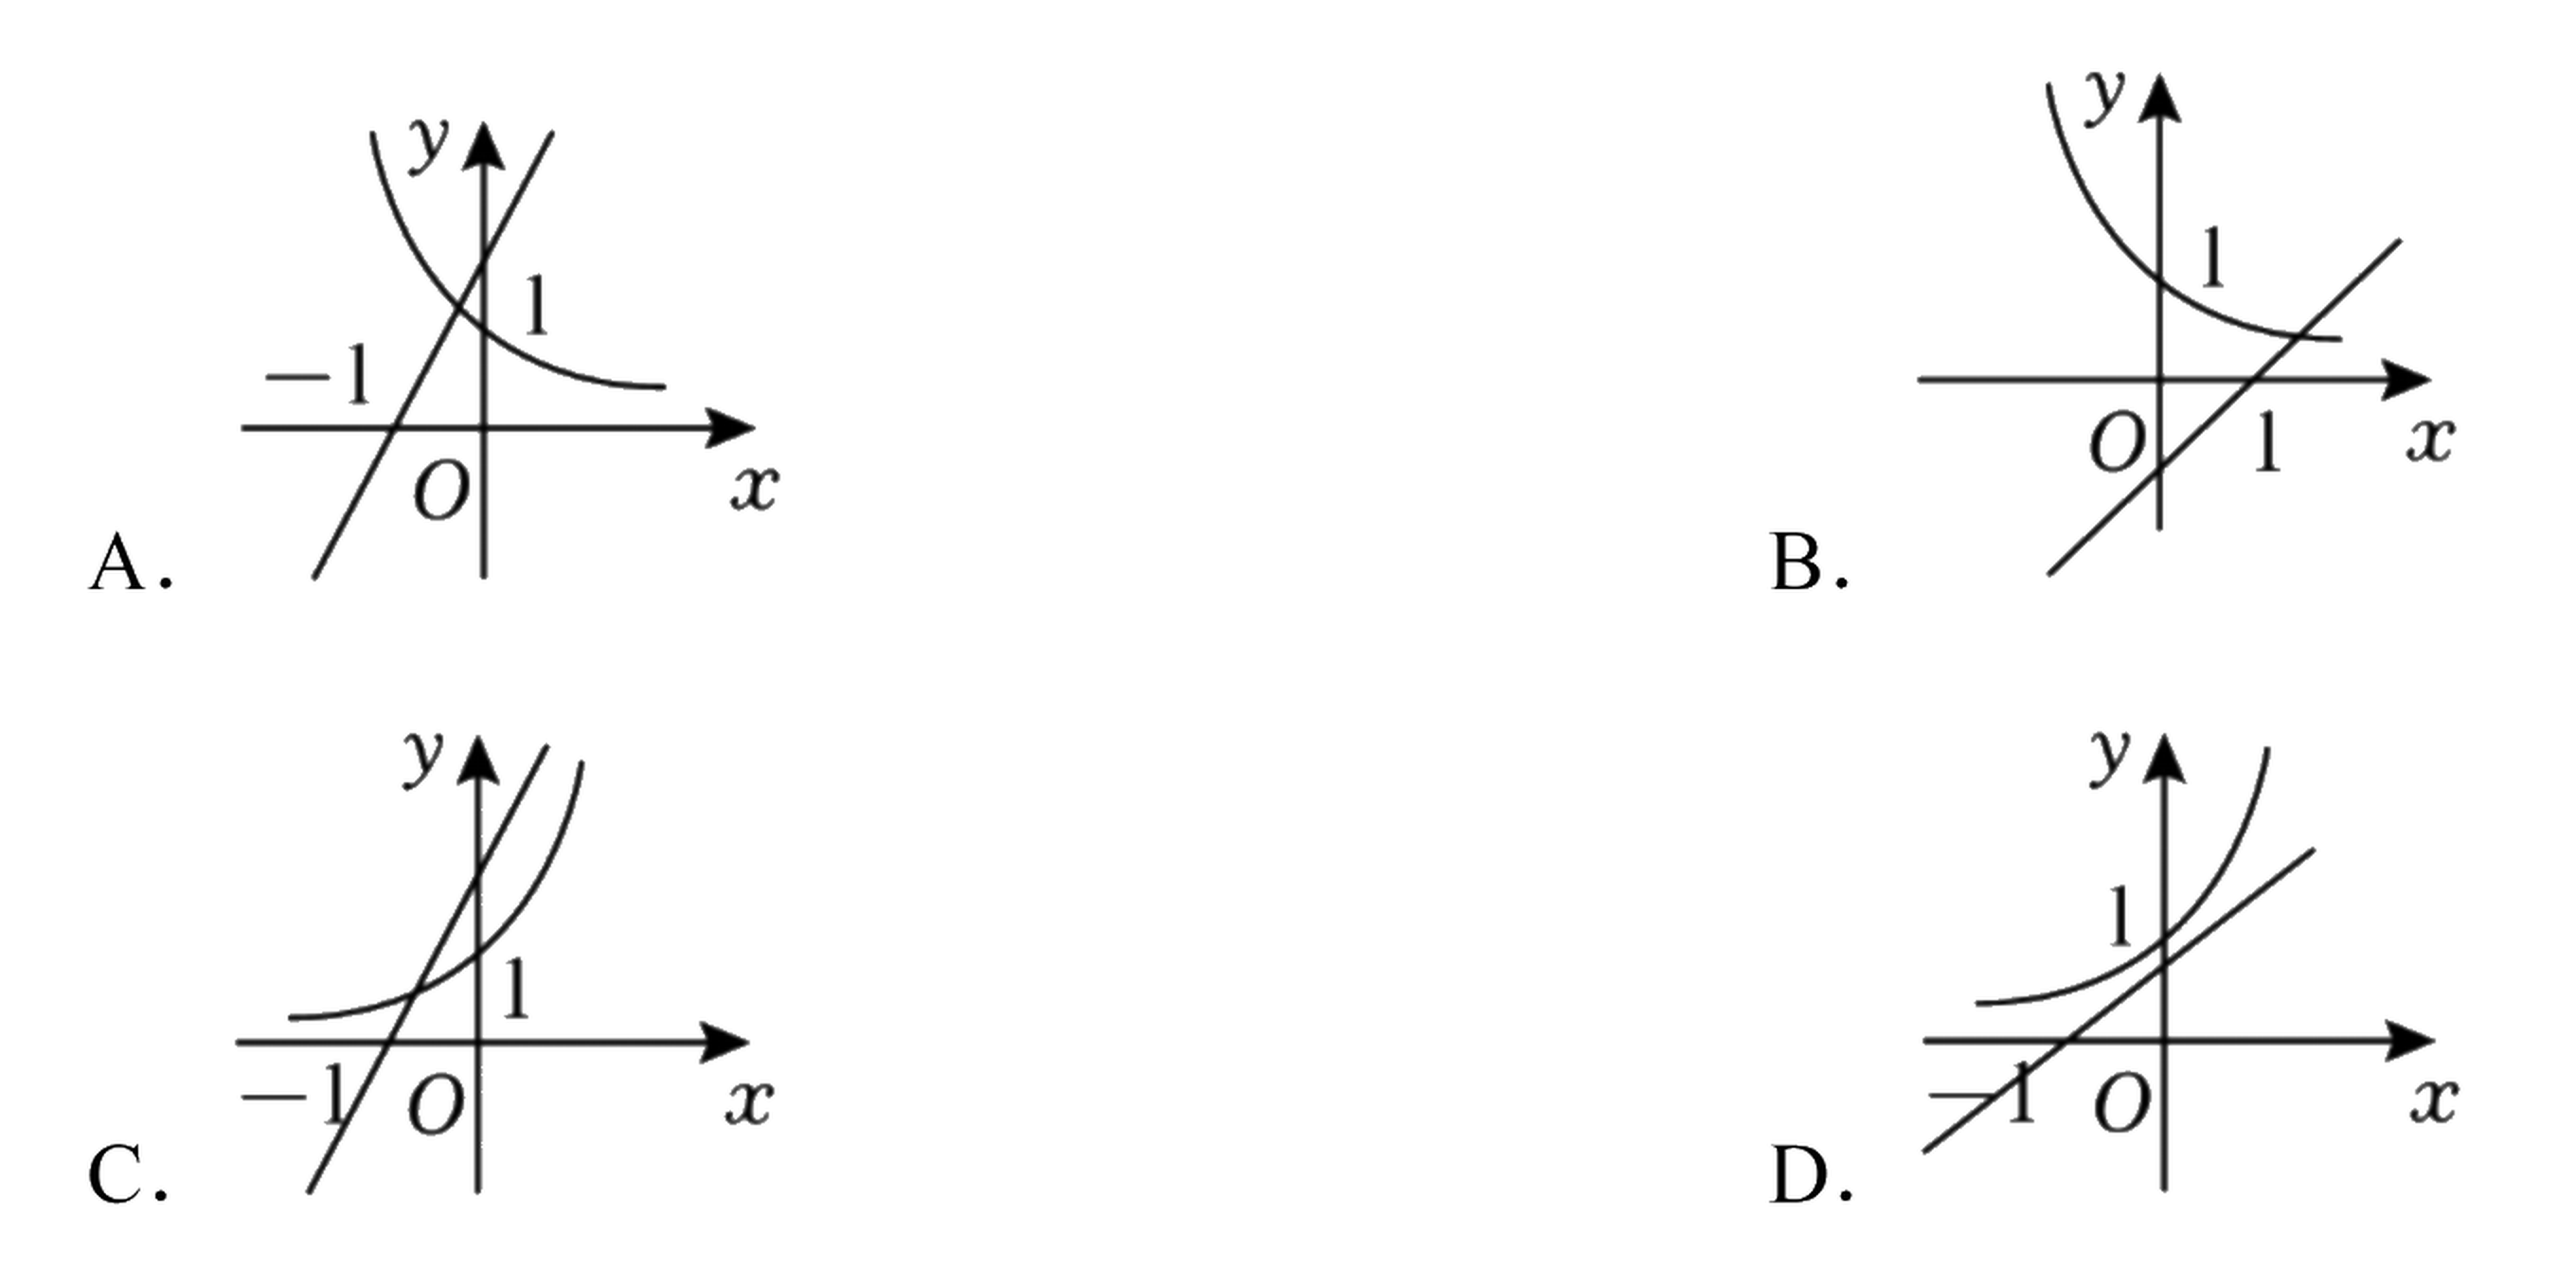
\includegraphics[width=0.80\textwidth]{figures/gao130_q15.png}
\end{center}

\ifanswer
\solbegin
\step{A 中，由指数函数 $y=a^x(a>0$ 且 $a\neq1)$ 图像递减得 $0<a<1$，}
\step{而一次函数 $y=a(x+1)$ 的图像与 $y$ 轴交点纵坐标为 $a>1$，二者矛盾，}
\step{所以 A 错；}
\step{由一次函数 $y=a(x+1)$ 的图像与 $x$ 轴交点横坐标为 $-1$，排除 B；}
\step{C 中，由指数函数 $y=a^x(a>0$ 且 $a\neq1)$ 图像递减得 $a>1$，}% 原卷"递减得 a>1"系笔误（应为"递增"），与 A 中"递减得 0<a<1"自相矛盾，照录
\step{而一次函数 $y=a(x+1)$ 的图像与 $y$ 轴交点纵坐标为 $a>1$，二者 $a$ 值吻合，}
\step{所以 C 对；}
\step{D 中，由一次函数 $y=a(x+1)$ 的图像得 $a=1$，与 $a>0$ 且 $a\neq1$ 矛盾，}
\step{所以 D 错.}
\step{故选 $C$.}
\solend
\fi

\item 设 $A_1$、$A_2$、$A_3$、$\cdots$、$A_7$ 是均含有 $2$ 个元素的集合，且 $A_1\cap A_7=\varnothing$，$A_i\cap A_{i+1}=\varnothing(i=1,2,3,\cdots,6)$，记 $B=A_1\cup A_2\cup A_3\cup\cdots\cup A_7$，则 $B$ 中元素个数的最小值是\mbox{（\quad）}

\keepwithprev
A. $4$\qquad B. $5$\qquad C. $6$\qquad D. $7$

\ifanswer
\solbegin
\step{取 $A_1=\{1,2\}$，$A_2=\{3,4\}$，$A_3=\{1,2\}$，$A_4=\{3,4\}$，$A_5=\{1,5\}$，$A_6=\{2,3\}$，$A_7=\{4,5\}$，}
\step{所以 $B$ 中元素个数的最小值是 $5$，故选 $B$.}
\solend
\fi

\end{enumerate}

\bigsec{三、解答题}

\begin{enumerate}
\setcounter{enumi}{16}

\item 已知全集为 $\R$，集合 $A=\{x\mid-2\leqslant x\leqslant5\}$，集合 $B=\{x\mid m-1\leqslant x\leqslant2m+1\}$．

(1) 求 $\overline{A}$；

(2) 若 $A\cup B=A$，求实数 $m$ 的取值范围．

\ifanswer
\solbegin
\step{(1) $(-\infty,-2)\cup(5,+\infty)$；}
\step{(2) 若 $A\cup B=A$，则 $B\subseteq A$，}
\step{当 $B=\varnothing$ 时，$m-1>2m+1$，解得 $m<-2$；}
\step{当 $B\neq\varnothing$ 时，$\begin{cases}m-1\leqslant2m+1\\m-1\geqslant-2\\2m+1\leqslant5\end{cases}$，解得 $-1\leqslant m\leqslant2$；}
\step{故实数 $m$ 的取值范围为 $\{m\mid-1\leqslant m\leqslant2$ 或 $m<-2\}$.}
\solend
\fi

\item 在不等式的应用中，有一些很基本而十分重要的不等式，如平均值不等式和三角不等式等，我们将其统称为基本不等式．

(1) 已知 $x$、$y$ 为正数，且 $2x+y=2$，求 $\dfrac1x+\dfrac2y$ 的最小值；

(2) 若关于 $x$ 的不等式 $\lvert x+1\rvert+\lvert2-x\rvert\geqslant a^2+a+1$ 对于一切实数 $x$ 都成立，求实数 $a$ 的取值范围．

\ifanswer
\solbegin
\step{(1) 因为 $x$、$y$ 为正数，且 $2x+y=2$，}
\step{所以 $\dfrac1x+\dfrac2y=\dfrac12\left(\dfrac1x+\dfrac2y\right)(2x+y)=\dfrac12\left(4+\dfrac yx+\dfrac{4x}y\right)\geqslant\dfrac12\left(4+2\sqrt{\dfrac yx\cdot\dfrac{4x}y}\right)=4$，}
\step{当且仅当 $\dfrac yx=\dfrac{4x}y$，即 $x=\dfrac12$，$y=1$ 时取等号，所以 $\dfrac1x+\dfrac2y$ 的最小值为 $4$；}
\step{(2) 由绝对值三角不等式得 $\lvert x+1\rvert+\lvert2-x\rvert\geqslant\lvert(x+1)+(2-x)\rvert=3$，}
\step{当且仅当 $-1\leqslant x\leqslant2$ 时取等号，所以 $\lvert x+1\rvert+\lvert2-x\rvert$ 的最小值为 $3$，}
\step{因为关于 $x$ 的不等式 $\lvert x+1\rvert+\lvert2-x\rvert\geqslant a^2+a+1$ 对于一切实数 $x$ 都成立，}
\step{所以 $a^2+a+1\leqslant3$，即 $a^2+a-2\leqslant0$，解得 $-2\leqslant a\leqslant1$，}
\step{所以实数 $a$ 的取值范围是 $[-2,1]$.}
\solend
\fi

\item 某医学专家为研究传染病传播中病毒细胞的发展规律，将病毒细胞注入一只小白鼠体内进行试验，经检测，病毒细胞的个数 $y$ 与天数 $x$ 的部分数据如表所示：

\begin{center}
\begin{tabular}{|c|c|c|c|c|c|c|c|}
\hline
天数 $(x)$ & $1$ & $2$ & $3$ & $4$ & $5$ & $6$ & $\cdots$ \\
\hline
病毒细胞的个数 $(y)$ & $1$ & $2$ & $4$ & $8$ & $16$ & $32$ & $\cdots$ \\
\hline
\end{tabular}
\end{center}

(1) 若病毒细胞的个数 $y$ 关于天数 $x$ 的变化规律可选用以下两个函数模型之一进行近似刻画：① $y=a\cdot b^x(a>0$，$b>0$，$b\neq1)$；② $y=a\cdot x^k(a\neq0)$．请结合表格中的数据，选择合适的函数模型，说明理由，并求出相应的函数表达式；

(2) 若该病毒细胞在小白鼠体内的个数超过 $10^8$，小白鼠将死亡，但注射某种药物，可杀死其体内 $98\%$ 的病毒细胞．则在 (1) 的条件下，为了使小白鼠在试验过程中不死亡，第一次最迟应在何时注射该种药物？（结果精确到天）

\ifanswer
\solbegin
\step{(1) 选择模型① $y=a\cdot b^x(a>0$，$b>0$，$b\neq1)$，理由如下：}
\step{观察表格数据，$y$ 的值随 $x$ 呈指数倍增：}
\step{$x=1$ 时，$y=1$，$x=2$ 时，$y=2$，$x=3$ 时，$y=4$，}
\step{后一天的病毒数是前一天的 $2$ 倍，符合指数增长的特征；}
\step{若选用幂函数模型 $y=a\cdot x^k$，代入前两组数据得 $a\cdot1^k=1$、$a\cdot2^k=2$，}
\step{解得 $a=1$，$k=1$，即 $y=x$，}
\step{但 $x=3$ 时，$y=3$ 与表格中 $y=4$ 严重不符，因此幂函数不匹配；}
\step{将 $(1,1)$ 代入 $y=a\cdot b^x$ 得 $a\cdot b=1$，}
\step{将 $(2,2)$ 代入得 $a\cdot b^2=2$，两式相除得 $b=2$，进而得 $a=\dfrac12$，}
\step{验证所有表格点均满足 $y=2^{x-1}$，最终函数表达式为 $y=2^{x-1}(x\in\N^*)$；}
\step{(2) 由题意得第一次注射药物前病毒细胞个数 $y$ 关于天数 $x(x\in\N^*)$ 的函数}
\step{关系式为 $y=2^{x-1}(x\in\N^*)$，}
\step{为了使小白鼠在试验过程中不死亡，则 $2^{x-1}\leqslant10^8$，}
\step{所以 $x-1\leqslant\log_210^8=8\log_210=\dfrac8{\lg2}$，解得 $x\leqslant1+\dfrac8{\lg2}\approx27.6$，}
\step{又 $x\in\N^*$，所以第一次最迟应在第 $27$ 天注射该种药物.}
\solend
\fi

\item 对在直角坐标系的第一象限内的任意两点 $(a,b)$，$(c,d)$ 作如下定义：$\dfrac ab>\dfrac cd$，那么称点 $(a,b)$ 是点 $(c,d)$ 的“上位点”，同时点 $(c,d)$ 是点 $(a,b)$ 的“下位点”．

(1) 试写出点 $(3,5)$ 的一个“上位点”坐标和一个“下位点”坐标；

(2) 设 $a$、$b$、$c$、$d$ 均为正数，且点 $(a,b)$ 是点 $(c,d)$ 的上位点，请判断点 $P(a+c,b+d)$ 是否既是点 $(a,b)$ 的“下位点”又是点 $(c,d)$ 的“上位点”，如果是，请证明；如果不是，请说明理由；

(3) 设正整数 $n$ 满足以下条件：对任意实数 $m\in\{t\mid0<t<4,t\in\Z\}$，总存在正整数 $k$，使得点 $(n,k)$ 既是点 $(4,m)$ 的“下位点”，又是点 $(5,m+1)$ 的“上位点”，求正整数 $n$ 的最小值．

\ifanswer
\solbegin
\step{(1) 由 $\dfrac34>\dfrac35>\dfrac36$ 得点 $(3,5)$ 的一个“上位点”的坐标为 $(3,4)$，}
\step{一个“下位点”的坐标为 $(3,6)$.}
\step{(2) 是，证明如下：}
\step{因为 $a$、$b$、$c$、$d$ 均为正数，点 $(a,b)$ 是点 $(c,d)$ 的“上位点”，}
\step{所以 $\dfrac ab>\dfrac cd$，所以 $ad>bc$，}
\step{因为 $\dfrac{a+c}{b+d}-\dfrac ab=\dfrac{b(a+c)-a(b+d)}{b(b+d)}=\dfrac{bc-ad}{b(b+d)}<0$，所以 $\dfrac{a+c}{b+d}<\dfrac ab$，}
\step{点 $P(a+c,b+d)$ 是点 $(a,b)$ 的“下位点”，}
\step{因为 $\dfrac{a+c}{b+d}-\dfrac cd=\dfrac{d(a+c)-c(b+d)}{d(b+d)}=\dfrac{ad-bc}{d(b+d)}>0$.}
\step{所以 $\dfrac{a+c}{b+d}>\dfrac cd$ 点 $P(a+c,b+d)$ 是点 $(c,d)$ 的“上位点”；}
\step{所以 $P(a+c,b+d)$ 既是点 $(a,b)$ 的“下位点”又是点 $(c,d)$ 的“上位点”；}
\step{(3) 由题意得 $m=1,2,3$，}
\step{由题意存在正整数 $k$：$\dfrac5{m+1}<\dfrac nk<\dfrac4m$，所以 $\begin{cases}\dfrac n4<k<\dfrac{2n}5(m=1)\\\dfrac n2<k<\dfrac{3n}5(m=2)\\\dfrac{3n}4<k<\dfrac{4n}5(m=3)\end{cases}$，}
\step{检验：$n=1,2,\cdots,8$ 不能同时找到整数 $k$，}
\step{$n=9$：$m=1$ 取 $k=3$，$m=2$ 取 $k=5$，$m=3$ 取 $k=7$，均满足，}
\step{所以正整数 $n$ 的最小值为 $9$.}
\solend
\fi

\end{enumerate}

\end{document}
"
%
% ① 原始材料：微信公众号"魔都数学加油站"文章，连载"27学年高一140"，原文标题
% "27学年高一140——2026-2027年上海市北郊高级中学高一上期中"；
% 原文链接：https://mp.weixin.qq.com/s/XBEYuTheiBoqu15dtLuD6A。
%   ★ 编号不一致说明：公众号连载号印"140"，与上一批已入库的"高一140 甘泉外国语"
%   （同一公众号另一篇文章、同为期中卷）撞号，系公众号笔误/重复。本仓库数字编号
%   02—143 中"高一130"一直空缺（连载 130 暂未见原文），故将本卷本地编号定为"高一130"、
%   填补该空缺，使数字编号连续（basename 全程为 高一130_北郊高级中学_期中）；
%   连载号 143 归正牌卷"上海中学 高一上期中"；本卷连载号仍印 140，见材料流转表。
%   卷面标题印"2026-2027 年北郊高级中学高一上期中"（卷面只有学校名、不含"上海市"、
%   不含任何期号/连载号），本稿照卷面录入；粉红色水印"魔都数学加油站"及页脚未录入。
% 正文为 9 张 PNG 页（01、04、05、06、09 为 2560x3620；02、03、07、08 为 4762x6735，
% 同一篇各页分辨率不同，逐页按各自分辨率放大核对），题目下印有【解析】，为讲评版。
% 题目、解析均据原图转录。
%
% 卷首标题：原卷印作"2026-2027 年北郊高级中学高一上期中"，年份区间按全稿惯例排
% en dash；原卷未印副标题，本卷为期中卷、跨集合与常用逻辑用语／不等式／函数三章，
% 按题目内容补出"集合与常用逻辑用语、不等式、函数"（与 125／126／128／129／131／132／133
% 同期中卷口径相同）。
%
% 题号体例：本卷共 18 题——一、填空题 3—12（10 题）、二、选择题 13—16（4 题）、
% 三、解答题 17—20（4 题）。三节分别 \setcounter{enumi}{2}／{12}／{16}。
% 原卷从第 3 题起、无第 1、2 题、**无第 21 题**（第 20 题解析续至 09 页，末行
% "所以正整数 n 的最小值为 9."，09 页下半页整片空白＋水印收尾、无第 10 页），本稿保留原题号。
%
% ② 与原卷的排版差异：
%   ① 原文从第 3 题起，本稿保留原题号；原卷止于第 20 题、无第 21 题、无附加题节；
%   ② 原卷每题下直接印【解析】，本稿按全稿惯例置于答案版；全卷 18 题均印【解析】、
%      无独立【答案】段，四道选择题答案在解析末句"故选 C／D／C／B"，括号
%      \mbox{（\quad）} 留空、不另提 \ans{}；全卷 0 处 \ans{}，答案版【解析】标记数 18＝题数；
%   ③ 原卷未印副标题，本稿按"知识模块"口径补出；
%   ④ 原卷填空横线按全稿惯例排为 \blankline[4.4em]；选择题括号排 \mbox{（\quad）}、
%      每个选项段前按惯例加 \keepwithprev；解答题不留作答区、不加 \anspace（讲评版）；
%   ⑤ 原卷数集排斜体 $R$／$N$，按全稿惯例改 \R／\N；空集记号 \varnothing；
%      绝对值排 \lvert…\rvert，集合描述竖线排 \mid；不等号按全稿惯例排 \leqslant／\geqslant；
%      补集照原卷上划线 \overline{A}；
%   ⑥ 1 幅插图 + 1 张印刷表格：第 15 题四幅坐标函数图象选项（04 页）取原卷截图
%      去粉色水印、去色、按原卷 2x2 排布合并为 figures/gao130_q15.png（非插图重绘），
%      放在 \keepwithprev 之后 \begin{center} 内、三版都出；第 19 题 (1) 印刷数据表格
%      （07 页，天数 x 1—6／病毒细胞个数 y 1/2/4/8/16/32）按原卷用 tabular 重排、
%      题干内三版都出（非插图）。
%      第 15 题是"二、选择题"节内带大图块的第三题（Q13 为节首题但无图），
%      在 \bigsec{二、选择题} 之前加 \needvspace{11cm} 连节标题一起量、Q15 \item 之前
%      加 \needvspace{9cm}——守卫必须放在 \bigsec 之前，放标题之后会让"二、选择题"
%      孤立在页末（B 类，照 高一26／40／59／136／140 成例）；三版切页审计均"合计异常：无"；
%   ⑦ 子题标号 (1)(2)(3) 原卷用半角括号，照录；圈数字 ①②③④ 照录；
%      数学式内半角逗号照录（如第 14 题 $(a>0,a\neq1)$、第 16 题
%      $(i=1,2,3,\cdots,6)$、第 20 题 $m=1,2,3$ 等）；
%      行末西文句点按全稿惯例照录；
%   ⑧ 题干中的中文弯引号按原卷照录（Q12"变项和"、Q20"上位点""下位点"等），
%      注释内一律 ASCII 引号；原卷"图像"用词逐处照录（Q9、Q15 均作"图像"）。
%
% ③ 行数复核：一条 \step = 原卷解析的一个印刷行（cases 块与 tabular 各作一个印刷行计）。
%   逐题 \step 条数，合计 98 条（Q3:3 Q4:2 Q5:2 Q6:1 Q7:1 Q8:3 Q9:5 Q10:10 Q11:6
%   Q12:7 Q13:1 Q14:2 Q15:10 Q16:2 Q17:5 Q18:8 Q19:15 Q20:15），与原卷印刷行逐题相等。
%
% ④ 判别式／子集符号结论：
%   判别式：全卷未出现判别式记号（无 $\Delta$、无 $\triangle$）；
%   子集符号：第 4 题题干"$B\subseteq A$"、第 4 题【解析】"$B\subseteq A$"、
%      第 17 题 (2)【解析】"$B\subseteq A$"三处原卷均印带下划线 $\subseteq$，逐处
%      放大核对、照录 \subseteq；全卷未出现单线 \subset。
%
% ⑤ 原卷存疑照录（均照录未改，正文对应处另有 % 注）：
%   ① 第 15 题【解析】"C 中，由指数函数 $y=a^x$ 图像递减得 $a>1$"——"递减"应为
%      "递增"之误（与同题 A 中"递减得 $0<a<1$"自相矛盾），原卷如此，照录并加注；
%   ② 第 16 题题干"$A_1\cap A_7=\varnothing$""$A_i\cap A_{i+1}=\varnothing$"
%      的空集记号与解析所列各集合逐处照录；
%   ③ 第 19 题 (2) 题干"可杀死其体内 98% 的病毒细胞"、解析 (2) 只按 $y=2^{x-1}$
%      与 $10^8$ 比较（未另计 98%），照录不补步。
%
% ⑥ 跨页续印按题合并：Q8 题干在 01 页末、解析在 02 页；Q9 题干在 02 页、
%   解析在 02 页；Q10 题干在 02 页、解析前 5 行在 02—03 页、后 5 行在 03 页；
%   Q12 题干跨 03 页、解析首 5 行在 03 页末、末行在 04 页；Q15 题干在 04 页、
%   四幅图与解析前段在 04 页、解析续在 05 页；Q17 解析跨 05—06 页；Q18 题干与
%   (1) 解析在 06 页、(2) 解析在 06—07 页；Q19 表格在 07 页、解析跨 07—08 页；
%   Q20 定义与三小问在 08 页、解析 (1)(2) 在 08—09 页、解析 (3) 在 09 页；
%   本稿按题连排，不丢行。
%
\documentclass[a4paper,11pt]{article}
\usepackage{common}

\begin{document}

\examtitlest[3]{2026--2027 年北郊高级中学高一上期中}{集合与常用逻辑用语、不等式、函数}

\bigsec{一、填空题}

\begin{enumerate}
\setcounter{enumi}{2}

\item 不等式 $\dfrac{x-3}{x+1}<2$ 的解集为\blankline[4.4em].

\ifanswer
\solbegin
\step{不等式 $\dfrac{x-3}{x+1}<2$ 可化为 $\dfrac{x-3}{x+1}-2<0$，即 $\dfrac{x-3-2(x+1)}{x+1}<0$，}
\step{化简为 $\dfrac{x+5}{x+1}>0$，解得 $x<-5$ 或 $x>-1$，}
\step{所以不等式的解集为 $\{x\mid x<-5$ 或 $x>-1\}$.}
\solend
\fi

\item 已知集合 $A=\{x\mid0<x<a\}$，$B=\{x\mid1<x<2\}$，若 $B\subseteq A$，则实数 $a$ 的取值范围为\blankline[4.4em].

\ifanswer
\solbegin
\step{已知集合 $A=\{x\mid0<x<a\}$，$B=\{x\mid1<x<2\}$，}
\step{若 $B\subseteq A$，则 $a\geqslant2$，所以实数 $a$ 的取值范围是 $\{a\mid a\geqslant2\}$.}
\solend
\fi

\item 已知关于 $x$ 的方程 $x^2+x+c=0$ 的两个实数根为 $x_1$、$x_2$，若 $x_1^2x_2+x_2^2x_1=3$，则实数 $c=$\blankline[4.4em].

\ifanswer
\solbegin
\step{由韦达定理得 $x_1+x_2=-1$，$x_1x_2=c$，所以 $x_1^2x_2+x_2^2x_1=(x_1+x_2)x_1x_2=-c=3$，}
\step{所以 $c=-3$.}
\solend
\fi

\item 已知 $10^x=3$，$10^y=64$，则 $10^{x-\frac y3}=$\blankline[4.4em].

\ifanswer
\solbegin
\step{$10^{x-\frac y3}=10^x\div\sqrt[3]{10^y}=\dfrac34$.}
\solend
\fi

\item 若 $\lg2=a$，则可用 $a$ 表示 $\log_280=$\blankline[4.4em].

\ifanswer
\solbegin
\step{$\log_280=\dfrac{\lg80}{\lg2}=\dfrac{\lg10+\lg8}{\lg2}=\dfrac{1+3\lg2}{\lg2}=\dfrac{1+3a}{a}$.}
\solend
\fi

\item 已知 $a+2b=1$，则 $3^a+9^b$ 的最小值为\blankline[4.4em].

\ifanswer
\solbegin
\step{因为 $a+2b=1$，所以 $3^a+9^b=3^a+3^{2b}\geqslant2\sqrt{3^a\cdot3^{2b}}=2\sqrt{3^{a+2b}}=2\sqrt3$，}
\step{当且仅当 $3^a=3^{2b}$，且 $a+2b=1$，即 $a=\dfrac12$，$b=\dfrac14$ 时取等号，}
\step{故最小值为 $2\sqrt3$.}
\solend
\fi

\item 下列函数的图像关于原点成中心对称，且在区间 $(0,+\infty)$ 上是严格增函数的是\blankline[4.4em]（请填写全部正确的序号）.

① $y=\sqrt{x}$；② $y=\sqrt[3]{x}$；③ $y=x^{\frac23}$；④ $y=x^{-\frac13}$.

\ifanswer
\solbegin
\step{① $y=\sqrt{x}$ 的定义域为 $[0,+\infty)$，故其图像不关于原点成中心对称，①错误；}
\step{② $y=\sqrt[3]{x}$ 是奇函数，且在区间 $(0,+\infty)$ 上是严格增函数，②正确；}
\step{③ $y=x^{\frac23}$ 是偶函数，其图像关于 $y$ 轴对称，不关于原点成中心对称，③错误；}
\step{④由于幂指数 $-\dfrac13<0$，故 $y=x^{-\frac13}$ 在区间 $(0,+\infty)$ 上是严格减函数，④错误.}
\step{故正确的是②.}
\solend
\fi

\item 设 $a>0$ 且 $a\neq1$，若函数 $y=a^{2x}+2a^x-3$ 在区间 $[-1,1]$ 上的最大值为 $21$，则实数 $a$ 的值为\blankline[4.4em].

\ifanswer
\solbegin
\step{令 $t=a^x$，$x\in[-1,1]$，}
\step{当 $a>1$ 时，$t=a^x$ 严格增，则 $t\in\left[\dfrac1a,a\right]$，}
\step{则函数 $y=t^2+2t-3$，对称轴为 $t=-1$，}
\step{所以函数 $y=t^2+2t-3$ 在 $\left[\dfrac1a,a\right]$ 上严格增，}
\step{所以当 $t=a$ 时，$y$ 取得最大值 $a^2+2a-3=21$，解得 $a=4$ 或 $-6$（舍去）；}
\step{当 $0<a<1$ 时，$t=a^x$ 严格减，则 $t\in\left[a,\dfrac1a\right]$，}
\step{则函数 $y=t^2+2t-3$，对称轴为 $t=-1$，}
\step{所以函数 $y=t^2+2t-3$ 在 $\left[a,\dfrac1a\right]$ 上严格增，}
\step{所以当 $t=\dfrac1a$ 时，$y$ 取得最大值 $\dfrac1{a^2}+\dfrac2a-3=21$，解得 $a=\dfrac14$ 或 $-\dfrac16$（舍去）；}
\step{综上所述，实数 $a$ 的值为 $4$ 或 $\dfrac14$.}
\solend
\fi

\item 在关于 $x$ 的不等式 $x^2+(m+1)x+m<0$ 的解集中恰有两个整数，则实数 $m$ 的取值范围是\blankline[4.4em].

\ifanswer
\solbegin
\step{关于 $x$ 的不等式 $x^2+(m+1)x+m<0$ 可化为 $(x+1)(x+m)<0$，}
\step{当 $m>1$ 时，$-m<-1$，解不等式得 $-m<x<-1$；}
\step{当 $m<1$ 时，$-m>-1$，解不等式得 $-1<x<-m$；}
\step{由不等式的解集中恰有两个整数，}
\step{则 $-4\leqslant-m<-3$ 或 $1<-m\leqslant2$，即 $3<m\leqslant4$ 或 $-2\leqslant m<-1$，}
\step{所以 $m$ 的取值范围是 $[-2,-1)\cup(3,4]$.}
\solend
\fi

\item 已知集合 $M$ 的元素均为正整数，定义集合 $M$ 的“变项和”为：将 $M$ 中每个元素 $m$ 都乘以 $(-1)^m$ 后再求和．若集合 $A=\{n\mid1\leqslant n\leqslant20,n\in\N\}$，则集合 $A$ 的所有非空子集的“变项和”的总和为\blankline[4.4em].

\ifanswer
\solbegin
\step{集合 $A=\{n\mid1\leqslant n\leqslant20,n\in\N\}$ 中一共有 $20$ 个元素，}
\step{固定选中 $k$，剩下 $19$ 个元素任选，共 $2^{19}$ 个子集包含 $k$，每个 $k$ 贡献 $(-1)^k\cdot k\cdot2^{19}$，}
\step{$A=\{1,2,\cdots,20\}$，}
\step{奇数 $k=1,3,\cdots,19$，共 $10$ 个，$(-1)^k\cdot k=-k$，}
\step{偶数 $k=2,4,\cdots,20$，共 $10$ 个，$(-1)^k\cdot k=k$，}
\step{所以集合 $A$ 的所有非空子集的“变项和”的总和}
\step{为 $S=2^{19}\times[(-1+2)+(-3+4)+\cdots+(-19+20)]=2^{19}\times10=524880$.}
\solend
\fi

\end{enumerate}

% 第 15 题四幅图是"二、选择题"节内大图块；守卫须放在 \bigsec 之前连节标题一起量，
% 否则"二、选择题"会孤立在页末（B 类，照 高一26／40／59／136／140 成例）
\needvspace{11cm}
\bigsec{二、选择题}

\begin{enumerate}
\setcounter{enumi}{12}

\item 设 $ab>0$，则“$a>b$”是“$\dfrac1a<\dfrac1b$”的\mbox{（\quad）}

\keepwithprev
A. 充分非必要条件\qquad B. 必要非充分条件

C. 充要条件\qquad D. 既非充分也非必要条件

\ifanswer
\solbegin
\step{因为 $ab>0$，所以 $a>b\Leftrightarrow\dfrac1a<\dfrac1b$，故选 $C$.}
\solend
\fi

\item 已知 $A=\log_ax$，$B=\log_ay(a>0,a\neq1)$，则 $\log_a\dfrac{x^2}{\sqrt y}=$\mbox{（\quad）}

\keepwithprev
A. $\dfrac{A^2}{\sqrt B}$\qquad B. $2A^2B$\qquad C. $4AB$\qquad D. $2A-\dfrac12B$

\ifanswer
\solbegin
\step{由已知得 $x=a^A$，$y=a^B$，}
\step{所以 $\log_a\dfrac{x^2}{\sqrt y}=\log_a\dfrac{(a^A)^2}{\sqrt{a^B}}=\log_a\dfrac{a^{2A}}{a^{\frac12B}}=\log_a a^{2A-\frac12B}=2A-\dfrac12B$. 故选 $D$.}
\solend
\fi

% 第 15 题四幅坐标函数图象选项是一整块，守卫放在 \item 之前
\needvspace{9cm}
\item 在同一平面直角坐标系中，指数函数 $y=a^x(a>0$ 且 $a\neq1)$ 和一次函数 $y=a(x+1)$ 的图像关系可能是\mbox{（\quad）}

\keepwithprev
\begin{center}
% 四幅坐标函数图象选项取原卷 04 页截图去粉色水印、去色，按原卷 2x2 排布合并为一张
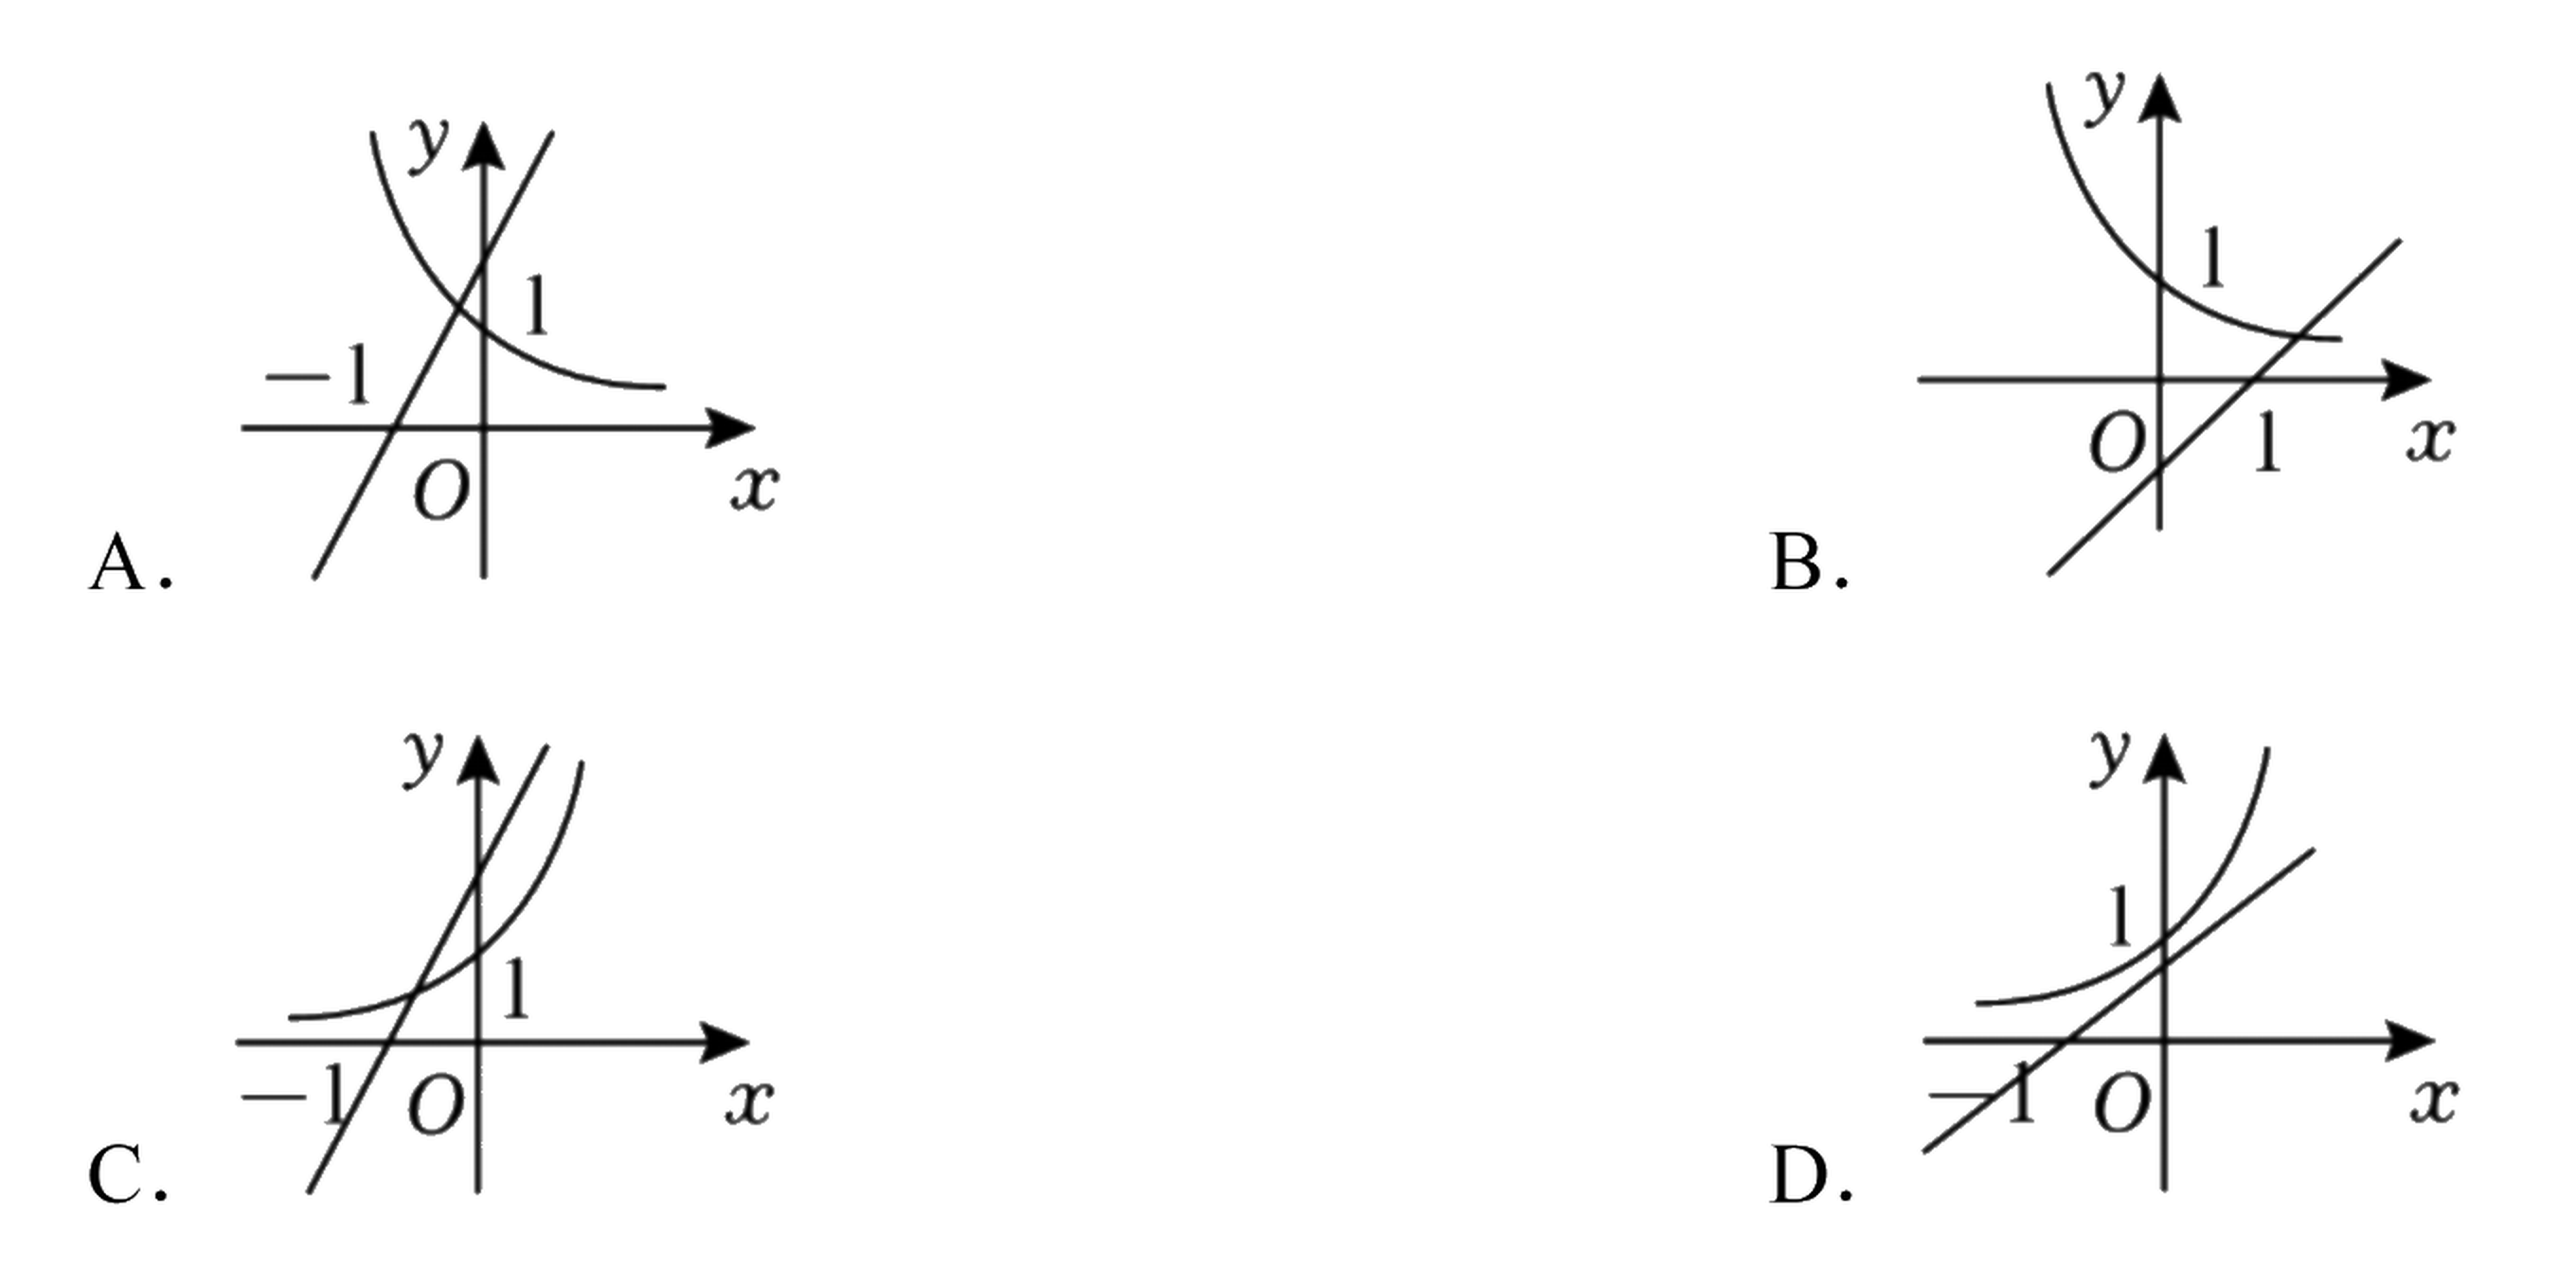
\includegraphics[width=0.80\textwidth]{figures/gao130_q15.png}
\end{center}

\ifanswer
\solbegin
\step{A 中，由指数函数 $y=a^x(a>0$ 且 $a\neq1)$ 图像递减得 $0<a<1$，}
\step{而一次函数 $y=a(x+1)$ 的图像与 $y$ 轴交点纵坐标为 $a>1$，二者矛盾，}
\step{所以 A 错；}
\step{由一次函数 $y=a(x+1)$ 的图像与 $x$ 轴交点横坐标为 $-1$，排除 B；}
\step{C 中，由指数函数 $y=a^x(a>0$ 且 $a\neq1)$ 图像递减得 $a>1$，}% 原卷"递减得 a>1"系笔误（应为"递增"），与 A 中"递减得 0<a<1"自相矛盾，照录
\step{而一次函数 $y=a(x+1)$ 的图像与 $y$ 轴交点纵坐标为 $a>1$，二者 $a$ 值吻合，}
\step{所以 C 对；}
\step{D 中，由一次函数 $y=a(x+1)$ 的图像得 $a=1$，与 $a>0$ 且 $a\neq1$ 矛盾，}
\step{所以 D 错.}
\step{故选 $C$.}
\solend
\fi

\item 设 $A_1$、$A_2$、$A_3$、$\cdots$、$A_7$ 是均含有 $2$ 个元素的集合，且 $A_1\cap A_7=\varnothing$，$A_i\cap A_{i+1}=\varnothing(i=1,2,3,\cdots,6)$，记 $B=A_1\cup A_2\cup A_3\cup\cdots\cup A_7$，则 $B$ 中元素个数的最小值是\mbox{（\quad）}

\keepwithprev
A. $4$\qquad B. $5$\qquad C. $6$\qquad D. $7$

\ifanswer
\solbegin
\step{取 $A_1=\{1,2\}$，$A_2=\{3,4\}$，$A_3=\{1,2\}$，$A_4=\{3,4\}$，$A_5=\{1,5\}$，$A_6=\{2,3\}$，$A_7=\{4,5\}$，}
\step{所以 $B$ 中元素个数的最小值是 $5$，故选 $B$.}
\solend
\fi

\end{enumerate}

\bigsec{三、解答题}

\begin{enumerate}
\setcounter{enumi}{16}

\item 已知全集为 $\R$，集合 $A=\{x\mid-2\leqslant x\leqslant5\}$，集合 $B=\{x\mid m-1\leqslant x\leqslant2m+1\}$．

(1) 求 $\overline{A}$；

(2) 若 $A\cup B=A$，求实数 $m$ 的取值范围．

\ifanswer
\solbegin
\step{(1) $(-\infty,-2)\cup(5,+\infty)$；}
\step{(2) 若 $A\cup B=A$，则 $B\subseteq A$，}
\step{当 $B=\varnothing$ 时，$m-1>2m+1$，解得 $m<-2$；}
\step{当 $B\neq\varnothing$ 时，$\begin{cases}m-1\leqslant2m+1\\m-1\geqslant-2\\2m+1\leqslant5\end{cases}$，解得 $-1\leqslant m\leqslant2$；}
\step{故实数 $m$ 的取值范围为 $\{m\mid-1\leqslant m\leqslant2$ 或 $m<-2\}$.}
\solend
\fi

\item 在不等式的应用中，有一些很基本而十分重要的不等式，如平均值不等式和三角不等式等，我们将其统称为基本不等式．

(1) 已知 $x$、$y$ 为正数，且 $2x+y=2$，求 $\dfrac1x+\dfrac2y$ 的最小值；

(2) 若关于 $x$ 的不等式 $\lvert x+1\rvert+\lvert2-x\rvert\geqslant a^2+a+1$ 对于一切实数 $x$ 都成立，求实数 $a$ 的取值范围．

\ifanswer
\solbegin
\step{(1) 因为 $x$、$y$ 为正数，且 $2x+y=2$，}
\step{所以 $\dfrac1x+\dfrac2y=\dfrac12\left(\dfrac1x+\dfrac2y\right)(2x+y)=\dfrac12\left(4+\dfrac yx+\dfrac{4x}y\right)\geqslant\dfrac12\left(4+2\sqrt{\dfrac yx\cdot\dfrac{4x}y}\right)=4$，}
\step{当且仅当 $\dfrac yx=\dfrac{4x}y$，即 $x=\dfrac12$，$y=1$ 时取等号，所以 $\dfrac1x+\dfrac2y$ 的最小值为 $4$；}
\step{(2) 由绝对值三角不等式得 $\lvert x+1\rvert+\lvert2-x\rvert\geqslant\lvert(x+1)+(2-x)\rvert=3$，}
\step{当且仅当 $-1\leqslant x\leqslant2$ 时取等号，所以 $\lvert x+1\rvert+\lvert2-x\rvert$ 的最小值为 $3$，}
\step{因为关于 $x$ 的不等式 $\lvert x+1\rvert+\lvert2-x\rvert\geqslant a^2+a+1$ 对于一切实数 $x$ 都成立，}
\step{所以 $a^2+a+1\leqslant3$，即 $a^2+a-2\leqslant0$，解得 $-2\leqslant a\leqslant1$，}
\step{所以实数 $a$ 的取值范围是 $[-2,1]$.}
\solend
\fi

\item 某医学专家为研究传染病传播中病毒细胞的发展规律，将病毒细胞注入一只小白鼠体内进行试验，经检测，病毒细胞的个数 $y$ 与天数 $x$ 的部分数据如表所示：

\begin{center}
\begin{tabular}{|c|c|c|c|c|c|c|c|}
\hline
天数 $(x)$ & $1$ & $2$ & $3$ & $4$ & $5$ & $6$ & $\cdots$ \\
\hline
病毒细胞的个数 $(y)$ & $1$ & $2$ & $4$ & $8$ & $16$ & $32$ & $\cdots$ \\
\hline
\end{tabular}
\end{center}

(1) 若病毒细胞的个数 $y$ 关于天数 $x$ 的变化规律可选用以下两个函数模型之一进行近似刻画：① $y=a\cdot b^x(a>0$，$b>0$，$b\neq1)$；② $y=a\cdot x^k(a\neq0)$．请结合表格中的数据，选择合适的函数模型，说明理由，并求出相应的函数表达式；

(2) 若该病毒细胞在小白鼠体内的个数超过 $10^8$，小白鼠将死亡，但注射某种药物，可杀死其体内 $98\%$ 的病毒细胞．则在 (1) 的条件下，为了使小白鼠在试验过程中不死亡，第一次最迟应在何时注射该种药物？（结果精确到天）

\ifanswer
\solbegin
\step{(1) 选择模型① $y=a\cdot b^x(a>0$，$b>0$，$b\neq1)$，理由如下：}
\step{观察表格数据，$y$ 的值随 $x$ 呈指数倍增：}
\step{$x=1$ 时，$y=1$，$x=2$ 时，$y=2$，$x=3$ 时，$y=4$，}
\step{后一天的病毒数是前一天的 $2$ 倍，符合指数增长的特征；}
\step{若选用幂函数模型 $y=a\cdot x^k$，代入前两组数据得 $a\cdot1^k=1$、$a\cdot2^k=2$，}
\step{解得 $a=1$，$k=1$，即 $y=x$，}
\step{但 $x=3$ 时，$y=3$ 与表格中 $y=4$ 严重不符，因此幂函数不匹配；}
\step{将 $(1,1)$ 代入 $y=a\cdot b^x$ 得 $a\cdot b=1$，}
\step{将 $(2,2)$ 代入得 $a\cdot b^2=2$，两式相除得 $b=2$，进而得 $a=\dfrac12$，}
\step{验证所有表格点均满足 $y=2^{x-1}$，最终函数表达式为 $y=2^{x-1}(x\in\N^*)$；}
\step{(2) 由题意得第一次注射药物前病毒细胞个数 $y$ 关于天数 $x(x\in\N^*)$ 的函数}
\step{关系式为 $y=2^{x-1}(x\in\N^*)$，}
\step{为了使小白鼠在试验过程中不死亡，则 $2^{x-1}\leqslant10^8$，}
\step{所以 $x-1\leqslant\log_210^8=8\log_210=\dfrac8{\lg2}$，解得 $x\leqslant1+\dfrac8{\lg2}\approx27.6$，}
\step{又 $x\in\N^*$，所以第一次最迟应在第 $27$ 天注射该种药物.}
\solend
\fi

\item 对在直角坐标系的第一象限内的任意两点 $(a,b)$，$(c,d)$ 作如下定义：$\dfrac ab>\dfrac cd$，那么称点 $(a,b)$ 是点 $(c,d)$ 的“上位点”，同时点 $(c,d)$ 是点 $(a,b)$ 的“下位点”．

(1) 试写出点 $(3,5)$ 的一个“上位点”坐标和一个“下位点”坐标；

(2) 设 $a$、$b$、$c$、$d$ 均为正数，且点 $(a,b)$ 是点 $(c,d)$ 的上位点，请判断点 $P(a+c,b+d)$ 是否既是点 $(a,b)$ 的“下位点”又是点 $(c,d)$ 的“上位点”，如果是，请证明；如果不是，请说明理由；

(3) 设正整数 $n$ 满足以下条件：对任意实数 $m\in\{t\mid0<t<4,t\in\Z\}$，总存在正整数 $k$，使得点 $(n,k)$ 既是点 $(4,m)$ 的“下位点”，又是点 $(5,m+1)$ 的“上位点”，求正整数 $n$ 的最小值．

\ifanswer
\solbegin
\step{(1) 由 $\dfrac34>\dfrac35>\dfrac36$ 得点 $(3,5)$ 的一个“上位点”的坐标为 $(3,4)$，}
\step{一个“下位点”的坐标为 $(3,6)$.}
\step{(2) 是，证明如下：}
\step{因为 $a$、$b$、$c$、$d$ 均为正数，点 $(a,b)$ 是点 $(c,d)$ 的“上位点”，}
\step{所以 $\dfrac ab>\dfrac cd$，所以 $ad>bc$，}
\step{因为 $\dfrac{a+c}{b+d}-\dfrac ab=\dfrac{b(a+c)-a(b+d)}{b(b+d)}=\dfrac{bc-ad}{b(b+d)}<0$，所以 $\dfrac{a+c}{b+d}<\dfrac ab$，}
\step{点 $P(a+c,b+d)$ 是点 $(a,b)$ 的“下位点”，}
\step{因为 $\dfrac{a+c}{b+d}-\dfrac cd=\dfrac{d(a+c)-c(b+d)}{d(b+d)}=\dfrac{ad-bc}{d(b+d)}>0$.}
\step{所以 $\dfrac{a+c}{b+d}>\dfrac cd$ 点 $P(a+c,b+d)$ 是点 $(c,d)$ 的“上位点”；}
\step{所以 $P(a+c,b+d)$ 既是点 $(a,b)$ 的“下位点”又是点 $(c,d)$ 的“上位点”；}
\step{(3) 由题意得 $m=1,2,3$，}
\step{由题意存在正整数 $k$：$\dfrac5{m+1}<\dfrac nk<\dfrac4m$，所以 $\begin{cases}\dfrac n4<k<\dfrac{2n}5(m=1)\\\dfrac n2<k<\dfrac{3n}5(m=2)\\\dfrac{3n}4<k<\dfrac{4n}5(m=3)\end{cases}$，}
\step{检验：$n=1,2,\cdots,8$ 不能同时找到整数 $k$，}
\step{$n=9$：$m=1$ 取 $k=3$，$m=2$ 取 $k=5$，$m=3$ 取 $k=7$，均满足，}
\step{所以正整数 $n$ 的最小值为 $9$.}
\solend
\fi

\end{enumerate}

\end{document}
"
% 紧凑版：xelatex "\def\iscompact{1}% 高一130_北郊高级中学_期中.tex
%   —— 高一上数学"2026-2027 年北郊高级中学高一上期中"（试卷版/答案版）
% 试卷版：xelatex 高一130_北郊高级中学_期中.tex
% 答案版：xelatex "\def\isanswer{1}% 高一130_北郊高级中学_期中.tex
%   —— 高一上数学"2026-2027 年北郊高级中学高一上期中"（试卷版/答案版）
% 试卷版：xelatex 高一130_北郊高级中学_期中.tex
% 答案版：xelatex "\def\isanswer{1}\input{高一130_北郊高级中学_期中.tex}"
% 紧凑版：xelatex "\def\iscompact{1}\input{高一130_北郊高级中学_期中.tex}"
%
% ① 原始材料：微信公众号"魔都数学加油站"文章，连载"27学年高一140"，原文标题
% "27学年高一140——2026-2027年上海市北郊高级中学高一上期中"；
% 原文链接：https://mp.weixin.qq.com/s/XBEYuTheiBoqu15dtLuD6A。
%   ★ 编号不一致说明：公众号连载号印"140"，与上一批已入库的"高一140 甘泉外国语"
%   （同一公众号另一篇文章、同为期中卷）撞号，系公众号笔误/重复。本仓库数字编号
%   02—143 中"高一130"一直空缺（连载 130 暂未见原文），故将本卷本地编号定为"高一130"、
%   填补该空缺，使数字编号连续（basename 全程为 高一130_北郊高级中学_期中）；
%   连载号 143 归正牌卷"上海中学 高一上期中"；本卷连载号仍印 140，见材料流转表。
%   卷面标题印"2026-2027 年北郊高级中学高一上期中"（卷面只有学校名、不含"上海市"、
%   不含任何期号/连载号），本稿照卷面录入；粉红色水印"魔都数学加油站"及页脚未录入。
% 正文为 9 张 PNG 页（01、04、05、06、09 为 2560x3620；02、03、07、08 为 4762x6735，
% 同一篇各页分辨率不同，逐页按各自分辨率放大核对），题目下印有【解析】，为讲评版。
% 题目、解析均据原图转录。
%
% 卷首标题：原卷印作"2026-2027 年北郊高级中学高一上期中"，年份区间按全稿惯例排
% en dash；原卷未印副标题，本卷为期中卷、跨集合与常用逻辑用语／不等式／函数三章，
% 按题目内容补出"集合与常用逻辑用语、不等式、函数"（与 125／126／128／129／131／132／133
% 同期中卷口径相同）。
%
% 题号体例：本卷共 18 题——一、填空题 3—12（10 题）、二、选择题 13—16（4 题）、
% 三、解答题 17—20（4 题）。三节分别 \setcounter{enumi}{2}／{12}／{16}。
% 原卷从第 3 题起、无第 1、2 题、**无第 21 题**（第 20 题解析续至 09 页，末行
% "所以正整数 n 的最小值为 9."，09 页下半页整片空白＋水印收尾、无第 10 页），本稿保留原题号。
%
% ② 与原卷的排版差异：
%   ① 原文从第 3 题起，本稿保留原题号；原卷止于第 20 题、无第 21 题、无附加题节；
%   ② 原卷每题下直接印【解析】，本稿按全稿惯例置于答案版；全卷 18 题均印【解析】、
%      无独立【答案】段，四道选择题答案在解析末句"故选 C／D／C／B"，括号
%      \mbox{（\quad）} 留空、不另提 \ans{}；全卷 0 处 \ans{}，答案版【解析】标记数 18＝题数；
%   ③ 原卷未印副标题，本稿按"知识模块"口径补出；
%   ④ 原卷填空横线按全稿惯例排为 \blankline[4.4em]；选择题括号排 \mbox{（\quad）}、
%      每个选项段前按惯例加 \keepwithprev；解答题不留作答区、不加 \anspace（讲评版）；
%   ⑤ 原卷数集排斜体 $R$／$N$，按全稿惯例改 \R／\N；空集记号 \varnothing；
%      绝对值排 \lvert…\rvert，集合描述竖线排 \mid；不等号按全稿惯例排 \leqslant／\geqslant；
%      补集照原卷上划线 \overline{A}；
%   ⑥ 1 幅插图 + 1 张印刷表格：第 15 题四幅坐标函数图象选项（04 页）取原卷截图
%      去粉色水印、去色、按原卷 2x2 排布合并为 figures/gao130_q15.png（非插图重绘），
%      放在 \keepwithprev 之后 \begin{center} 内、三版都出；第 19 题 (1) 印刷数据表格
%      （07 页，天数 x 1—6／病毒细胞个数 y 1/2/4/8/16/32）按原卷用 tabular 重排、
%      题干内三版都出（非插图）。
%      第 15 题是"二、选择题"节内带大图块的第三题（Q13 为节首题但无图），
%      在 \bigsec{二、选择题} 之前加 \needvspace{11cm} 连节标题一起量、Q15 \item 之前
%      加 \needvspace{9cm}——守卫必须放在 \bigsec 之前，放标题之后会让"二、选择题"
%      孤立在页末（B 类，照 高一26／40／59／136／140 成例）；三版切页审计均"合计异常：无"；
%   ⑦ 子题标号 (1)(2)(3) 原卷用半角括号，照录；圈数字 ①②③④ 照录；
%      数学式内半角逗号照录（如第 14 题 $(a>0,a\neq1)$、第 16 题
%      $(i=1,2,3,\cdots,6)$、第 20 题 $m=1,2,3$ 等）；
%      行末西文句点按全稿惯例照录；
%   ⑧ 题干中的中文弯引号按原卷照录（Q12"变项和"、Q20"上位点""下位点"等），
%      注释内一律 ASCII 引号；原卷"图像"用词逐处照录（Q9、Q15 均作"图像"）。
%
% ③ 行数复核：一条 \step = 原卷解析的一个印刷行（cases 块与 tabular 各作一个印刷行计）。
%   逐题 \step 条数，合计 98 条（Q3:3 Q4:2 Q5:2 Q6:1 Q7:1 Q8:3 Q9:5 Q10:10 Q11:6
%   Q12:7 Q13:1 Q14:2 Q15:10 Q16:2 Q17:5 Q18:8 Q19:15 Q20:15），与原卷印刷行逐题相等。
%
% ④ 判别式／子集符号结论：
%   判别式：全卷未出现判别式记号（无 $\Delta$、无 $\triangle$）；
%   子集符号：第 4 题题干"$B\subseteq A$"、第 4 题【解析】"$B\subseteq A$"、
%      第 17 题 (2)【解析】"$B\subseteq A$"三处原卷均印带下划线 $\subseteq$，逐处
%      放大核对、照录 \subseteq；全卷未出现单线 \subset。
%
% ⑤ 原卷存疑照录（均照录未改，正文对应处另有 % 注）：
%   ① 第 15 题【解析】"C 中，由指数函数 $y=a^x$ 图像递减得 $a>1$"——"递减"应为
%      "递增"之误（与同题 A 中"递减得 $0<a<1$"自相矛盾），原卷如此，照录并加注；
%   ② 第 16 题题干"$A_1\cap A_7=\varnothing$""$A_i\cap A_{i+1}=\varnothing$"
%      的空集记号与解析所列各集合逐处照录；
%   ③ 第 19 题 (2) 题干"可杀死其体内 98% 的病毒细胞"、解析 (2) 只按 $y=2^{x-1}$
%      与 $10^8$ 比较（未另计 98%），照录不补步。
%
% ⑥ 跨页续印按题合并：Q8 题干在 01 页末、解析在 02 页；Q9 题干在 02 页、
%   解析在 02 页；Q10 题干在 02 页、解析前 5 行在 02—03 页、后 5 行在 03 页；
%   Q12 题干跨 03 页、解析首 5 行在 03 页末、末行在 04 页；Q15 题干在 04 页、
%   四幅图与解析前段在 04 页、解析续在 05 页；Q17 解析跨 05—06 页；Q18 题干与
%   (1) 解析在 06 页、(2) 解析在 06—07 页；Q19 表格在 07 页、解析跨 07—08 页；
%   Q20 定义与三小问在 08 页、解析 (1)(2) 在 08—09 页、解析 (3) 在 09 页；
%   本稿按题连排，不丢行。
%
\documentclass[a4paper,11pt]{article}
\usepackage{common}

\begin{document}

\examtitlest[3]{2026--2027 年北郊高级中学高一上期中}{集合与常用逻辑用语、不等式、函数}

\bigsec{一、填空题}

\begin{enumerate}
\setcounter{enumi}{2}

\item 不等式 $\dfrac{x-3}{x+1}<2$ 的解集为\blankline[4.4em].

\ifanswer
\solbegin
\step{不等式 $\dfrac{x-3}{x+1}<2$ 可化为 $\dfrac{x-3}{x+1}-2<0$，即 $\dfrac{x-3-2(x+1)}{x+1}<0$，}
\step{化简为 $\dfrac{x+5}{x+1}>0$，解得 $x<-5$ 或 $x>-1$，}
\step{所以不等式的解集为 $\{x\mid x<-5$ 或 $x>-1\}$.}
\solend
\fi

\item 已知集合 $A=\{x\mid0<x<a\}$，$B=\{x\mid1<x<2\}$，若 $B\subseteq A$，则实数 $a$ 的取值范围为\blankline[4.4em].

\ifanswer
\solbegin
\step{已知集合 $A=\{x\mid0<x<a\}$，$B=\{x\mid1<x<2\}$，}
\step{若 $B\subseteq A$，则 $a\geqslant2$，所以实数 $a$ 的取值范围是 $\{a\mid a\geqslant2\}$.}
\solend
\fi

\item 已知关于 $x$ 的方程 $x^2+x+c=0$ 的两个实数根为 $x_1$、$x_2$，若 $x_1^2x_2+x_2^2x_1=3$，则实数 $c=$\blankline[4.4em].

\ifanswer
\solbegin
\step{由韦达定理得 $x_1+x_2=-1$，$x_1x_2=c$，所以 $x_1^2x_2+x_2^2x_1=(x_1+x_2)x_1x_2=-c=3$，}
\step{所以 $c=-3$.}
\solend
\fi

\item 已知 $10^x=3$，$10^y=64$，则 $10^{x-\frac y3}=$\blankline[4.4em].

\ifanswer
\solbegin
\step{$10^{x-\frac y3}=10^x\div\sqrt[3]{10^y}=\dfrac34$.}
\solend
\fi

\item 若 $\lg2=a$，则可用 $a$ 表示 $\log_280=$\blankline[4.4em].

\ifanswer
\solbegin
\step{$\log_280=\dfrac{\lg80}{\lg2}=\dfrac{\lg10+\lg8}{\lg2}=\dfrac{1+3\lg2}{\lg2}=\dfrac{1+3a}{a}$.}
\solend
\fi

\item 已知 $a+2b=1$，则 $3^a+9^b$ 的最小值为\blankline[4.4em].

\ifanswer
\solbegin
\step{因为 $a+2b=1$，所以 $3^a+9^b=3^a+3^{2b}\geqslant2\sqrt{3^a\cdot3^{2b}}=2\sqrt{3^{a+2b}}=2\sqrt3$，}
\step{当且仅当 $3^a=3^{2b}$，且 $a+2b=1$，即 $a=\dfrac12$，$b=\dfrac14$ 时取等号，}
\step{故最小值为 $2\sqrt3$.}
\solend
\fi

\item 下列函数的图像关于原点成中心对称，且在区间 $(0,+\infty)$ 上是严格增函数的是\blankline[4.4em]（请填写全部正确的序号）.

① $y=\sqrt{x}$；② $y=\sqrt[3]{x}$；③ $y=x^{\frac23}$；④ $y=x^{-\frac13}$.

\ifanswer
\solbegin
\step{① $y=\sqrt{x}$ 的定义域为 $[0,+\infty)$，故其图像不关于原点成中心对称，①错误；}
\step{② $y=\sqrt[3]{x}$ 是奇函数，且在区间 $(0,+\infty)$ 上是严格增函数，②正确；}
\step{③ $y=x^{\frac23}$ 是偶函数，其图像关于 $y$ 轴对称，不关于原点成中心对称，③错误；}
\step{④由于幂指数 $-\dfrac13<0$，故 $y=x^{-\frac13}$ 在区间 $(0,+\infty)$ 上是严格减函数，④错误.}
\step{故正确的是②.}
\solend
\fi

\item 设 $a>0$ 且 $a\neq1$，若函数 $y=a^{2x}+2a^x-3$ 在区间 $[-1,1]$ 上的最大值为 $21$，则实数 $a$ 的值为\blankline[4.4em].

\ifanswer
\solbegin
\step{令 $t=a^x$，$x\in[-1,1]$，}
\step{当 $a>1$ 时，$t=a^x$ 严格增，则 $t\in\left[\dfrac1a,a\right]$，}
\step{则函数 $y=t^2+2t-3$，对称轴为 $t=-1$，}
\step{所以函数 $y=t^2+2t-3$ 在 $\left[\dfrac1a,a\right]$ 上严格增，}
\step{所以当 $t=a$ 时，$y$ 取得最大值 $a^2+2a-3=21$，解得 $a=4$ 或 $-6$（舍去）；}
\step{当 $0<a<1$ 时，$t=a^x$ 严格减，则 $t\in\left[a,\dfrac1a\right]$，}
\step{则函数 $y=t^2+2t-3$，对称轴为 $t=-1$，}
\step{所以函数 $y=t^2+2t-3$ 在 $\left[a,\dfrac1a\right]$ 上严格增，}
\step{所以当 $t=\dfrac1a$ 时，$y$ 取得最大值 $\dfrac1{a^2}+\dfrac2a-3=21$，解得 $a=\dfrac14$ 或 $-\dfrac16$（舍去）；}
\step{综上所述，实数 $a$ 的值为 $4$ 或 $\dfrac14$.}
\solend
\fi

\item 在关于 $x$ 的不等式 $x^2+(m+1)x+m<0$ 的解集中恰有两个整数，则实数 $m$ 的取值范围是\blankline[4.4em].

\ifanswer
\solbegin
\step{关于 $x$ 的不等式 $x^2+(m+1)x+m<0$ 可化为 $(x+1)(x+m)<0$，}
\step{当 $m>1$ 时，$-m<-1$，解不等式得 $-m<x<-1$；}
\step{当 $m<1$ 时，$-m>-1$，解不等式得 $-1<x<-m$；}
\step{由不等式的解集中恰有两个整数，}
\step{则 $-4\leqslant-m<-3$ 或 $1<-m\leqslant2$，即 $3<m\leqslant4$ 或 $-2\leqslant m<-1$，}
\step{所以 $m$ 的取值范围是 $[-2,-1)\cup(3,4]$.}
\solend
\fi

\item 已知集合 $M$ 的元素均为正整数，定义集合 $M$ 的“变项和”为：将 $M$ 中每个元素 $m$ 都乘以 $(-1)^m$ 后再求和．若集合 $A=\{n\mid1\leqslant n\leqslant20,n\in\N\}$，则集合 $A$ 的所有非空子集的“变项和”的总和为\blankline[4.4em].

\ifanswer
\solbegin
\step{集合 $A=\{n\mid1\leqslant n\leqslant20,n\in\N\}$ 中一共有 $20$ 个元素，}
\step{固定选中 $k$，剩下 $19$ 个元素任选，共 $2^{19}$ 个子集包含 $k$，每个 $k$ 贡献 $(-1)^k\cdot k\cdot2^{19}$，}
\step{$A=\{1,2,\cdots,20\}$，}
\step{奇数 $k=1,3,\cdots,19$，共 $10$ 个，$(-1)^k\cdot k=-k$，}
\step{偶数 $k=2,4,\cdots,20$，共 $10$ 个，$(-1)^k\cdot k=k$，}
\step{所以集合 $A$ 的所有非空子集的“变项和”的总和}
\step{为 $S=2^{19}\times[(-1+2)+(-3+4)+\cdots+(-19+20)]=2^{19}\times10=524880$.}
\solend
\fi

\end{enumerate}

% 第 15 题四幅图是"二、选择题"节内大图块；守卫须放在 \bigsec 之前连节标题一起量，
% 否则"二、选择题"会孤立在页末（B 类，照 高一26／40／59／136／140 成例）
\needvspace{11cm}
\bigsec{二、选择题}

\begin{enumerate}
\setcounter{enumi}{12}

\item 设 $ab>0$，则“$a>b$”是“$\dfrac1a<\dfrac1b$”的\mbox{（\quad）}

\keepwithprev
A. 充分非必要条件\qquad B. 必要非充分条件

C. 充要条件\qquad D. 既非充分也非必要条件

\ifanswer
\solbegin
\step{因为 $ab>0$，所以 $a>b\Leftrightarrow\dfrac1a<\dfrac1b$，故选 $C$.}
\solend
\fi

\item 已知 $A=\log_ax$，$B=\log_ay(a>0,a\neq1)$，则 $\log_a\dfrac{x^2}{\sqrt y}=$\mbox{（\quad）}

\keepwithprev
A. $\dfrac{A^2}{\sqrt B}$\qquad B. $2A^2B$\qquad C. $4AB$\qquad D. $2A-\dfrac12B$

\ifanswer
\solbegin
\step{由已知得 $x=a^A$，$y=a^B$，}
\step{所以 $\log_a\dfrac{x^2}{\sqrt y}=\log_a\dfrac{(a^A)^2}{\sqrt{a^B}}=\log_a\dfrac{a^{2A}}{a^{\frac12B}}=\log_a a^{2A-\frac12B}=2A-\dfrac12B$. 故选 $D$.}
\solend
\fi

% 第 15 题四幅坐标函数图象选项是一整块，守卫放在 \item 之前
\needvspace{9cm}
\item 在同一平面直角坐标系中，指数函数 $y=a^x(a>0$ 且 $a\neq1)$ 和一次函数 $y=a(x+1)$ 的图像关系可能是\mbox{（\quad）}

\keepwithprev
\begin{center}
% 四幅坐标函数图象选项取原卷 04 页截图去粉色水印、去色，按原卷 2x2 排布合并为一张
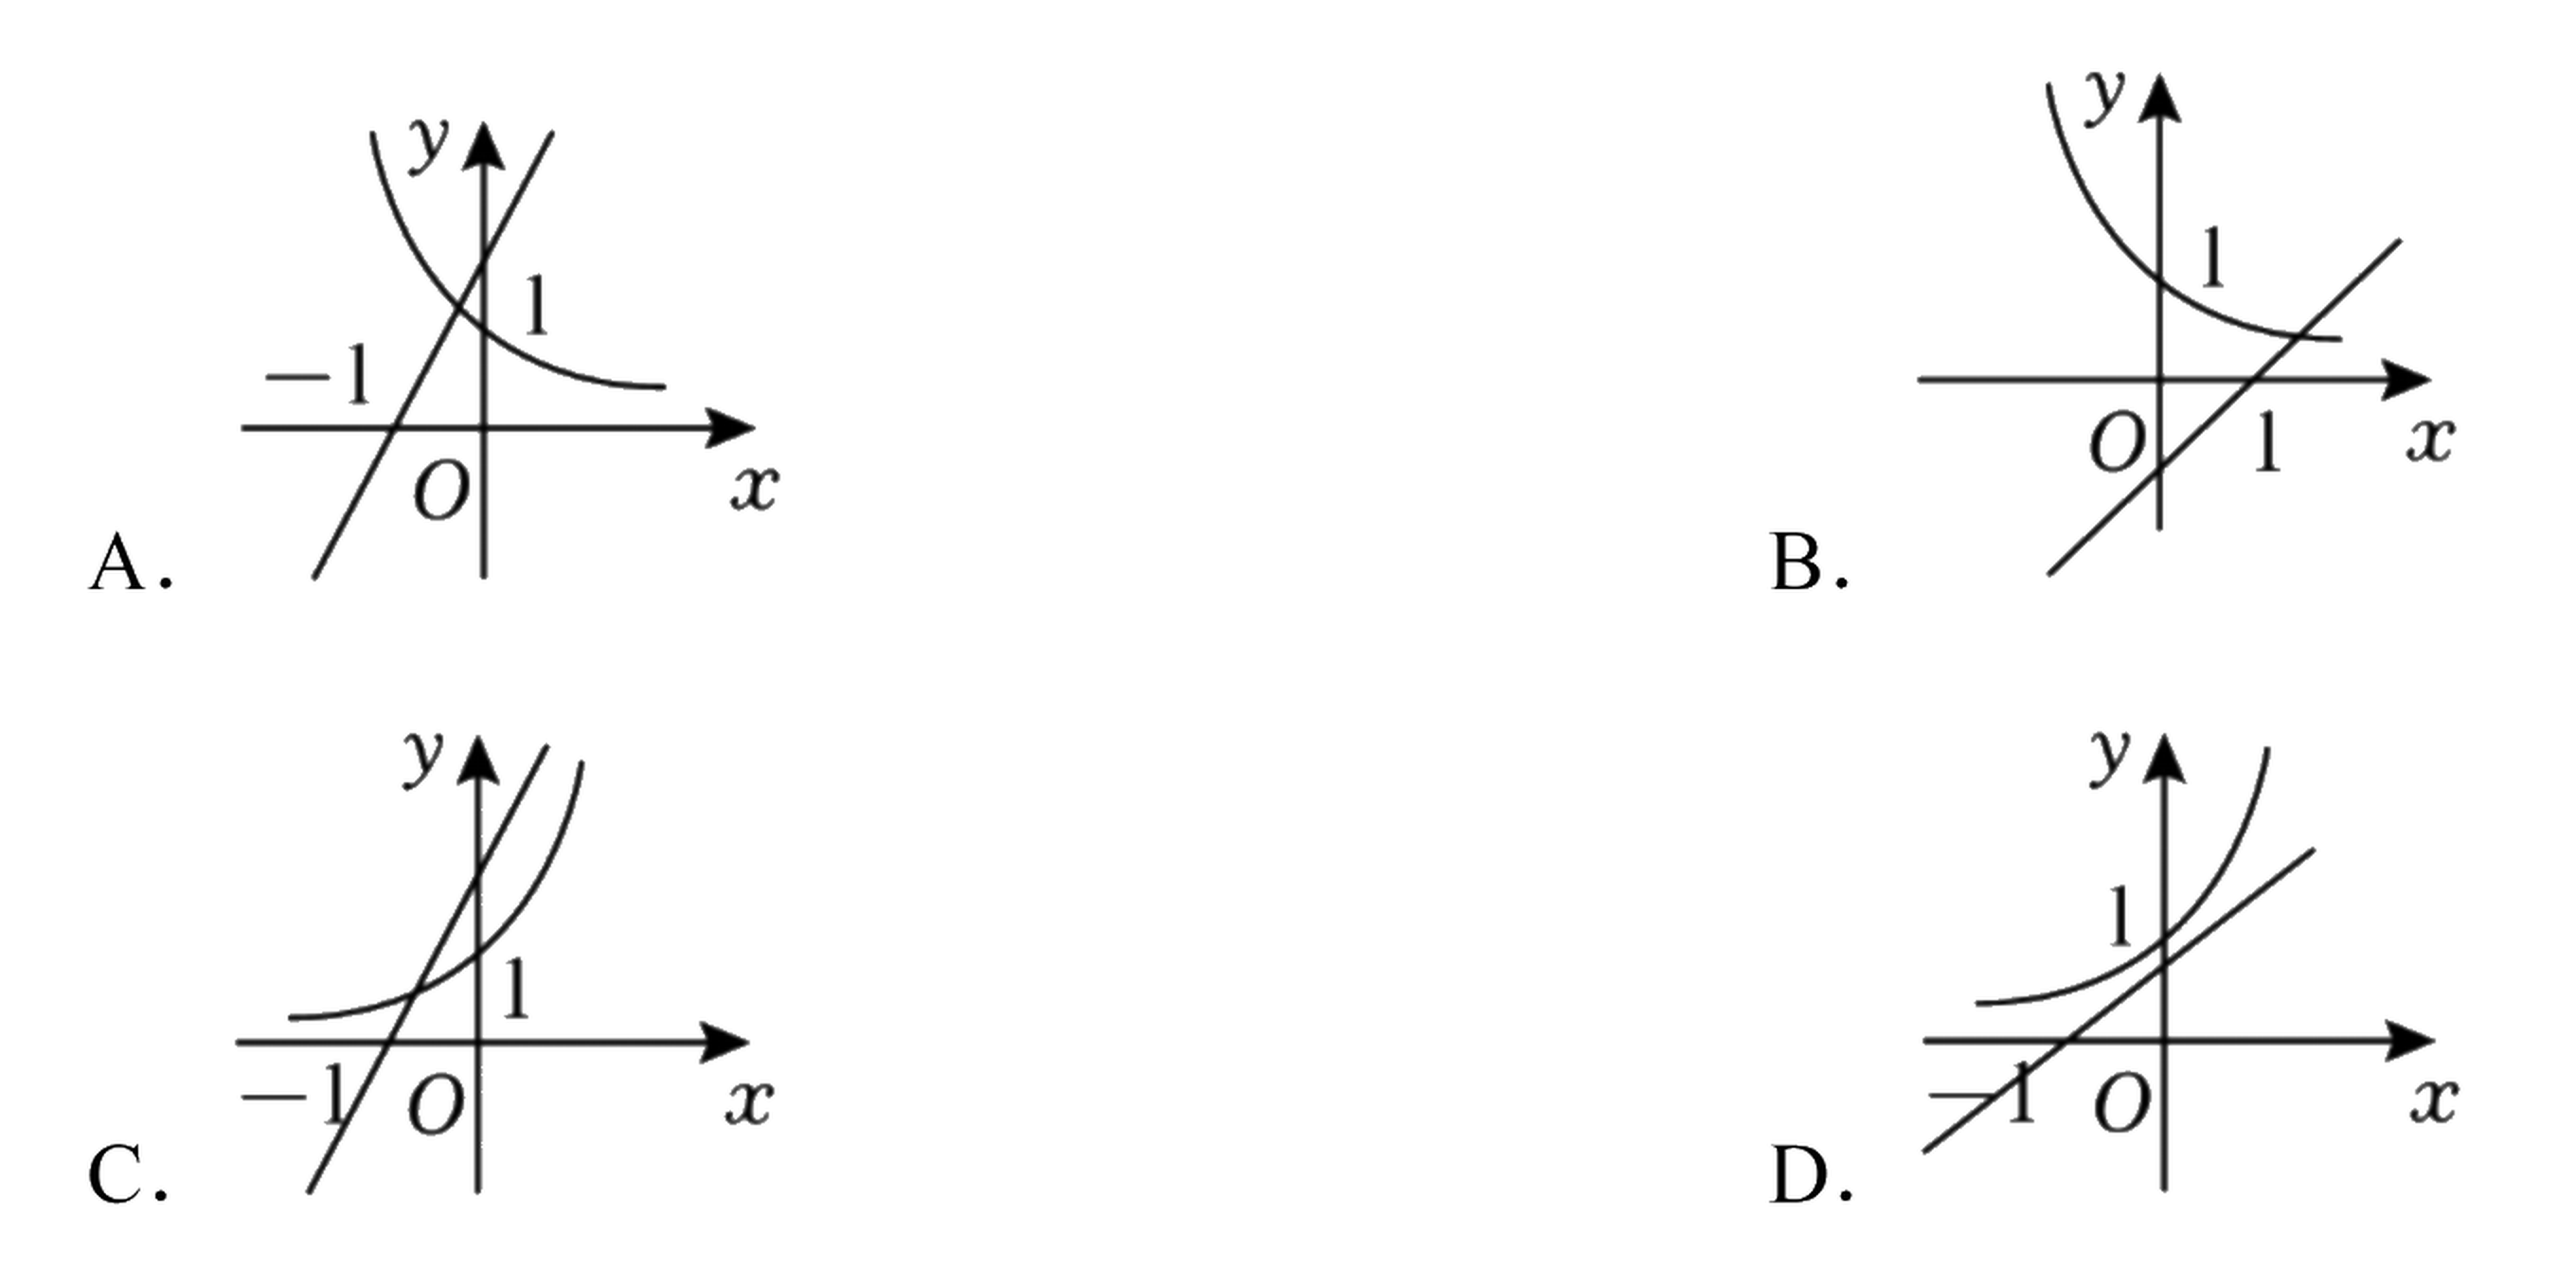
\includegraphics[width=0.80\textwidth]{figures/gao130_q15.png}
\end{center}

\ifanswer
\solbegin
\step{A 中，由指数函数 $y=a^x(a>0$ 且 $a\neq1)$ 图像递减得 $0<a<1$，}
\step{而一次函数 $y=a(x+1)$ 的图像与 $y$ 轴交点纵坐标为 $a>1$，二者矛盾，}
\step{所以 A 错；}
\step{由一次函数 $y=a(x+1)$ 的图像与 $x$ 轴交点横坐标为 $-1$，排除 B；}
\step{C 中，由指数函数 $y=a^x(a>0$ 且 $a\neq1)$ 图像递减得 $a>1$，}% 原卷"递减得 a>1"系笔误（应为"递增"），与 A 中"递减得 0<a<1"自相矛盾，照录
\step{而一次函数 $y=a(x+1)$ 的图像与 $y$ 轴交点纵坐标为 $a>1$，二者 $a$ 值吻合，}
\step{所以 C 对；}
\step{D 中，由一次函数 $y=a(x+1)$ 的图像得 $a=1$，与 $a>0$ 且 $a\neq1$ 矛盾，}
\step{所以 D 错.}
\step{故选 $C$.}
\solend
\fi

\item 设 $A_1$、$A_2$、$A_3$、$\cdots$、$A_7$ 是均含有 $2$ 个元素的集合，且 $A_1\cap A_7=\varnothing$，$A_i\cap A_{i+1}=\varnothing(i=1,2,3,\cdots,6)$，记 $B=A_1\cup A_2\cup A_3\cup\cdots\cup A_7$，则 $B$ 中元素个数的最小值是\mbox{（\quad）}

\keepwithprev
A. $4$\qquad B. $5$\qquad C. $6$\qquad D. $7$

\ifanswer
\solbegin
\step{取 $A_1=\{1,2\}$，$A_2=\{3,4\}$，$A_3=\{1,2\}$，$A_4=\{3,4\}$，$A_5=\{1,5\}$，$A_6=\{2,3\}$，$A_7=\{4,5\}$，}
\step{所以 $B$ 中元素个数的最小值是 $5$，故选 $B$.}
\solend
\fi

\end{enumerate}

\bigsec{三、解答题}

\begin{enumerate}
\setcounter{enumi}{16}

\item 已知全集为 $\R$，集合 $A=\{x\mid-2\leqslant x\leqslant5\}$，集合 $B=\{x\mid m-1\leqslant x\leqslant2m+1\}$．

(1) 求 $\overline{A}$；

(2) 若 $A\cup B=A$，求实数 $m$ 的取值范围．

\ifanswer
\solbegin
\step{(1) $(-\infty,-2)\cup(5,+\infty)$；}
\step{(2) 若 $A\cup B=A$，则 $B\subseteq A$，}
\step{当 $B=\varnothing$ 时，$m-1>2m+1$，解得 $m<-2$；}
\step{当 $B\neq\varnothing$ 时，$\begin{cases}m-1\leqslant2m+1\\m-1\geqslant-2\\2m+1\leqslant5\end{cases}$，解得 $-1\leqslant m\leqslant2$；}
\step{故实数 $m$ 的取值范围为 $\{m\mid-1\leqslant m\leqslant2$ 或 $m<-2\}$.}
\solend
\fi

\item 在不等式的应用中，有一些很基本而十分重要的不等式，如平均值不等式和三角不等式等，我们将其统称为基本不等式．

(1) 已知 $x$、$y$ 为正数，且 $2x+y=2$，求 $\dfrac1x+\dfrac2y$ 的最小值；

(2) 若关于 $x$ 的不等式 $\lvert x+1\rvert+\lvert2-x\rvert\geqslant a^2+a+1$ 对于一切实数 $x$ 都成立，求实数 $a$ 的取值范围．

\ifanswer
\solbegin
\step{(1) 因为 $x$、$y$ 为正数，且 $2x+y=2$，}
\step{所以 $\dfrac1x+\dfrac2y=\dfrac12\left(\dfrac1x+\dfrac2y\right)(2x+y)=\dfrac12\left(4+\dfrac yx+\dfrac{4x}y\right)\geqslant\dfrac12\left(4+2\sqrt{\dfrac yx\cdot\dfrac{4x}y}\right)=4$，}
\step{当且仅当 $\dfrac yx=\dfrac{4x}y$，即 $x=\dfrac12$，$y=1$ 时取等号，所以 $\dfrac1x+\dfrac2y$ 的最小值为 $4$；}
\step{(2) 由绝对值三角不等式得 $\lvert x+1\rvert+\lvert2-x\rvert\geqslant\lvert(x+1)+(2-x)\rvert=3$，}
\step{当且仅当 $-1\leqslant x\leqslant2$ 时取等号，所以 $\lvert x+1\rvert+\lvert2-x\rvert$ 的最小值为 $3$，}
\step{因为关于 $x$ 的不等式 $\lvert x+1\rvert+\lvert2-x\rvert\geqslant a^2+a+1$ 对于一切实数 $x$ 都成立，}
\step{所以 $a^2+a+1\leqslant3$，即 $a^2+a-2\leqslant0$，解得 $-2\leqslant a\leqslant1$，}
\step{所以实数 $a$ 的取值范围是 $[-2,1]$.}
\solend
\fi

\item 某医学专家为研究传染病传播中病毒细胞的发展规律，将病毒细胞注入一只小白鼠体内进行试验，经检测，病毒细胞的个数 $y$ 与天数 $x$ 的部分数据如表所示：

\begin{center}
\begin{tabular}{|c|c|c|c|c|c|c|c|}
\hline
天数 $(x)$ & $1$ & $2$ & $3$ & $4$ & $5$ & $6$ & $\cdots$ \\
\hline
病毒细胞的个数 $(y)$ & $1$ & $2$ & $4$ & $8$ & $16$ & $32$ & $\cdots$ \\
\hline
\end{tabular}
\end{center}

(1) 若病毒细胞的个数 $y$ 关于天数 $x$ 的变化规律可选用以下两个函数模型之一进行近似刻画：① $y=a\cdot b^x(a>0$，$b>0$，$b\neq1)$；② $y=a\cdot x^k(a\neq0)$．请结合表格中的数据，选择合适的函数模型，说明理由，并求出相应的函数表达式；

(2) 若该病毒细胞在小白鼠体内的个数超过 $10^8$，小白鼠将死亡，但注射某种药物，可杀死其体内 $98\%$ 的病毒细胞．则在 (1) 的条件下，为了使小白鼠在试验过程中不死亡，第一次最迟应在何时注射该种药物？（结果精确到天）

\ifanswer
\solbegin
\step{(1) 选择模型① $y=a\cdot b^x(a>0$，$b>0$，$b\neq1)$，理由如下：}
\step{观察表格数据，$y$ 的值随 $x$ 呈指数倍增：}
\step{$x=1$ 时，$y=1$，$x=2$ 时，$y=2$，$x=3$ 时，$y=4$，}
\step{后一天的病毒数是前一天的 $2$ 倍，符合指数增长的特征；}
\step{若选用幂函数模型 $y=a\cdot x^k$，代入前两组数据得 $a\cdot1^k=1$、$a\cdot2^k=2$，}
\step{解得 $a=1$，$k=1$，即 $y=x$，}
\step{但 $x=3$ 时，$y=3$ 与表格中 $y=4$ 严重不符，因此幂函数不匹配；}
\step{将 $(1,1)$ 代入 $y=a\cdot b^x$ 得 $a\cdot b=1$，}
\step{将 $(2,2)$ 代入得 $a\cdot b^2=2$，两式相除得 $b=2$，进而得 $a=\dfrac12$，}
\step{验证所有表格点均满足 $y=2^{x-1}$，最终函数表达式为 $y=2^{x-1}(x\in\N^*)$；}
\step{(2) 由题意得第一次注射药物前病毒细胞个数 $y$ 关于天数 $x(x\in\N^*)$ 的函数}
\step{关系式为 $y=2^{x-1}(x\in\N^*)$，}
\step{为了使小白鼠在试验过程中不死亡，则 $2^{x-1}\leqslant10^8$，}
\step{所以 $x-1\leqslant\log_210^8=8\log_210=\dfrac8{\lg2}$，解得 $x\leqslant1+\dfrac8{\lg2}\approx27.6$，}
\step{又 $x\in\N^*$，所以第一次最迟应在第 $27$ 天注射该种药物.}
\solend
\fi

\item 对在直角坐标系的第一象限内的任意两点 $(a,b)$，$(c,d)$ 作如下定义：$\dfrac ab>\dfrac cd$，那么称点 $(a,b)$ 是点 $(c,d)$ 的“上位点”，同时点 $(c,d)$ 是点 $(a,b)$ 的“下位点”．

(1) 试写出点 $(3,5)$ 的一个“上位点”坐标和一个“下位点”坐标；

(2) 设 $a$、$b$、$c$、$d$ 均为正数，且点 $(a,b)$ 是点 $(c,d)$ 的上位点，请判断点 $P(a+c,b+d)$ 是否既是点 $(a,b)$ 的“下位点”又是点 $(c,d)$ 的“上位点”，如果是，请证明；如果不是，请说明理由；

(3) 设正整数 $n$ 满足以下条件：对任意实数 $m\in\{t\mid0<t<4,t\in\Z\}$，总存在正整数 $k$，使得点 $(n,k)$ 既是点 $(4,m)$ 的“下位点”，又是点 $(5,m+1)$ 的“上位点”，求正整数 $n$ 的最小值．

\ifanswer
\solbegin
\step{(1) 由 $\dfrac34>\dfrac35>\dfrac36$ 得点 $(3,5)$ 的一个“上位点”的坐标为 $(3,4)$，}
\step{一个“下位点”的坐标为 $(3,6)$.}
\step{(2) 是，证明如下：}
\step{因为 $a$、$b$、$c$、$d$ 均为正数，点 $(a,b)$ 是点 $(c,d)$ 的“上位点”，}
\step{所以 $\dfrac ab>\dfrac cd$，所以 $ad>bc$，}
\step{因为 $\dfrac{a+c}{b+d}-\dfrac ab=\dfrac{b(a+c)-a(b+d)}{b(b+d)}=\dfrac{bc-ad}{b(b+d)}<0$，所以 $\dfrac{a+c}{b+d}<\dfrac ab$，}
\step{点 $P(a+c,b+d)$ 是点 $(a,b)$ 的“下位点”，}
\step{因为 $\dfrac{a+c}{b+d}-\dfrac cd=\dfrac{d(a+c)-c(b+d)}{d(b+d)}=\dfrac{ad-bc}{d(b+d)}>0$.}
\step{所以 $\dfrac{a+c}{b+d}>\dfrac cd$ 点 $P(a+c,b+d)$ 是点 $(c,d)$ 的“上位点”；}
\step{所以 $P(a+c,b+d)$ 既是点 $(a,b)$ 的“下位点”又是点 $(c,d)$ 的“上位点”；}
\step{(3) 由题意得 $m=1,2,3$，}
\step{由题意存在正整数 $k$：$\dfrac5{m+1}<\dfrac nk<\dfrac4m$，所以 $\begin{cases}\dfrac n4<k<\dfrac{2n}5(m=1)\\\dfrac n2<k<\dfrac{3n}5(m=2)\\\dfrac{3n}4<k<\dfrac{4n}5(m=3)\end{cases}$，}
\step{检验：$n=1,2,\cdots,8$ 不能同时找到整数 $k$，}
\step{$n=9$：$m=1$ 取 $k=3$，$m=2$ 取 $k=5$，$m=3$ 取 $k=7$，均满足，}
\step{所以正整数 $n$ 的最小值为 $9$.}
\solend
\fi

\end{enumerate}

\end{document}
"
% 紧凑版：xelatex "\def\iscompact{1}% 高一130_北郊高级中学_期中.tex
%   —— 高一上数学"2026-2027 年北郊高级中学高一上期中"（试卷版/答案版）
% 试卷版：xelatex 高一130_北郊高级中学_期中.tex
% 答案版：xelatex "\def\isanswer{1}\input{高一130_北郊高级中学_期中.tex}"
% 紧凑版：xelatex "\def\iscompact{1}\input{高一130_北郊高级中学_期中.tex}"
%
% ① 原始材料：微信公众号"魔都数学加油站"文章，连载"27学年高一140"，原文标题
% "27学年高一140——2026-2027年上海市北郊高级中学高一上期中"；
% 原文链接：https://mp.weixin.qq.com/s/XBEYuTheiBoqu15dtLuD6A。
%   ★ 编号不一致说明：公众号连载号印"140"，与上一批已入库的"高一140 甘泉外国语"
%   （同一公众号另一篇文章、同为期中卷）撞号，系公众号笔误/重复。本仓库数字编号
%   02—143 中"高一130"一直空缺（连载 130 暂未见原文），故将本卷本地编号定为"高一130"、
%   填补该空缺，使数字编号连续（basename 全程为 高一130_北郊高级中学_期中）；
%   连载号 143 归正牌卷"上海中学 高一上期中"；本卷连载号仍印 140，见材料流转表。
%   卷面标题印"2026-2027 年北郊高级中学高一上期中"（卷面只有学校名、不含"上海市"、
%   不含任何期号/连载号），本稿照卷面录入；粉红色水印"魔都数学加油站"及页脚未录入。
% 正文为 9 张 PNG 页（01、04、05、06、09 为 2560x3620；02、03、07、08 为 4762x6735，
% 同一篇各页分辨率不同，逐页按各自分辨率放大核对），题目下印有【解析】，为讲评版。
% 题目、解析均据原图转录。
%
% 卷首标题：原卷印作"2026-2027 年北郊高级中学高一上期中"，年份区间按全稿惯例排
% en dash；原卷未印副标题，本卷为期中卷、跨集合与常用逻辑用语／不等式／函数三章，
% 按题目内容补出"集合与常用逻辑用语、不等式、函数"（与 125／126／128／129／131／132／133
% 同期中卷口径相同）。
%
% 题号体例：本卷共 18 题——一、填空题 3—12（10 题）、二、选择题 13—16（4 题）、
% 三、解答题 17—20（4 题）。三节分别 \setcounter{enumi}{2}／{12}／{16}。
% 原卷从第 3 题起、无第 1、2 题、**无第 21 题**（第 20 题解析续至 09 页，末行
% "所以正整数 n 的最小值为 9."，09 页下半页整片空白＋水印收尾、无第 10 页），本稿保留原题号。
%
% ② 与原卷的排版差异：
%   ① 原文从第 3 题起，本稿保留原题号；原卷止于第 20 题、无第 21 题、无附加题节；
%   ② 原卷每题下直接印【解析】，本稿按全稿惯例置于答案版；全卷 18 题均印【解析】、
%      无独立【答案】段，四道选择题答案在解析末句"故选 C／D／C／B"，括号
%      \mbox{（\quad）} 留空、不另提 \ans{}；全卷 0 处 \ans{}，答案版【解析】标记数 18＝题数；
%   ③ 原卷未印副标题，本稿按"知识模块"口径补出；
%   ④ 原卷填空横线按全稿惯例排为 \blankline[4.4em]；选择题括号排 \mbox{（\quad）}、
%      每个选项段前按惯例加 \keepwithprev；解答题不留作答区、不加 \anspace（讲评版）；
%   ⑤ 原卷数集排斜体 $R$／$N$，按全稿惯例改 \R／\N；空集记号 \varnothing；
%      绝对值排 \lvert…\rvert，集合描述竖线排 \mid；不等号按全稿惯例排 \leqslant／\geqslant；
%      补集照原卷上划线 \overline{A}；
%   ⑥ 1 幅插图 + 1 张印刷表格：第 15 题四幅坐标函数图象选项（04 页）取原卷截图
%      去粉色水印、去色、按原卷 2x2 排布合并为 figures/gao130_q15.png（非插图重绘），
%      放在 \keepwithprev 之后 \begin{center} 内、三版都出；第 19 题 (1) 印刷数据表格
%      （07 页，天数 x 1—6／病毒细胞个数 y 1/2/4/8/16/32）按原卷用 tabular 重排、
%      题干内三版都出（非插图）。
%      第 15 题是"二、选择题"节内带大图块的第三题（Q13 为节首题但无图），
%      在 \bigsec{二、选择题} 之前加 \needvspace{11cm} 连节标题一起量、Q15 \item 之前
%      加 \needvspace{9cm}——守卫必须放在 \bigsec 之前，放标题之后会让"二、选择题"
%      孤立在页末（B 类，照 高一26／40／59／136／140 成例）；三版切页审计均"合计异常：无"；
%   ⑦ 子题标号 (1)(2)(3) 原卷用半角括号，照录；圈数字 ①②③④ 照录；
%      数学式内半角逗号照录（如第 14 题 $(a>0,a\neq1)$、第 16 题
%      $(i=1,2,3,\cdots,6)$、第 20 题 $m=1,2,3$ 等）；
%      行末西文句点按全稿惯例照录；
%   ⑧ 题干中的中文弯引号按原卷照录（Q12"变项和"、Q20"上位点""下位点"等），
%      注释内一律 ASCII 引号；原卷"图像"用词逐处照录（Q9、Q15 均作"图像"）。
%
% ③ 行数复核：一条 \step = 原卷解析的一个印刷行（cases 块与 tabular 各作一个印刷行计）。
%   逐题 \step 条数，合计 98 条（Q3:3 Q4:2 Q5:2 Q6:1 Q7:1 Q8:3 Q9:5 Q10:10 Q11:6
%   Q12:7 Q13:1 Q14:2 Q15:10 Q16:2 Q17:5 Q18:8 Q19:15 Q20:15），与原卷印刷行逐题相等。
%
% ④ 判别式／子集符号结论：
%   判别式：全卷未出现判别式记号（无 $\Delta$、无 $\triangle$）；
%   子集符号：第 4 题题干"$B\subseteq A$"、第 4 题【解析】"$B\subseteq A$"、
%      第 17 题 (2)【解析】"$B\subseteq A$"三处原卷均印带下划线 $\subseteq$，逐处
%      放大核对、照录 \subseteq；全卷未出现单线 \subset。
%
% ⑤ 原卷存疑照录（均照录未改，正文对应处另有 % 注）：
%   ① 第 15 题【解析】"C 中，由指数函数 $y=a^x$ 图像递减得 $a>1$"——"递减"应为
%      "递增"之误（与同题 A 中"递减得 $0<a<1$"自相矛盾），原卷如此，照录并加注；
%   ② 第 16 题题干"$A_1\cap A_7=\varnothing$""$A_i\cap A_{i+1}=\varnothing$"
%      的空集记号与解析所列各集合逐处照录；
%   ③ 第 19 题 (2) 题干"可杀死其体内 98% 的病毒细胞"、解析 (2) 只按 $y=2^{x-1}$
%      与 $10^8$ 比较（未另计 98%），照录不补步。
%
% ⑥ 跨页续印按题合并：Q8 题干在 01 页末、解析在 02 页；Q9 题干在 02 页、
%   解析在 02 页；Q10 题干在 02 页、解析前 5 行在 02—03 页、后 5 行在 03 页；
%   Q12 题干跨 03 页、解析首 5 行在 03 页末、末行在 04 页；Q15 题干在 04 页、
%   四幅图与解析前段在 04 页、解析续在 05 页；Q17 解析跨 05—06 页；Q18 题干与
%   (1) 解析在 06 页、(2) 解析在 06—07 页；Q19 表格在 07 页、解析跨 07—08 页；
%   Q20 定义与三小问在 08 页、解析 (1)(2) 在 08—09 页、解析 (3) 在 09 页；
%   本稿按题连排，不丢行。
%
\documentclass[a4paper,11pt]{article}
\usepackage{common}

\begin{document}

\examtitlest[3]{2026--2027 年北郊高级中学高一上期中}{集合与常用逻辑用语、不等式、函数}

\bigsec{一、填空题}

\begin{enumerate}
\setcounter{enumi}{2}

\item 不等式 $\dfrac{x-3}{x+1}<2$ 的解集为\blankline[4.4em].

\ifanswer
\solbegin
\step{不等式 $\dfrac{x-3}{x+1}<2$ 可化为 $\dfrac{x-3}{x+1}-2<0$，即 $\dfrac{x-3-2(x+1)}{x+1}<0$，}
\step{化简为 $\dfrac{x+5}{x+1}>0$，解得 $x<-5$ 或 $x>-1$，}
\step{所以不等式的解集为 $\{x\mid x<-5$ 或 $x>-1\}$.}
\solend
\fi

\item 已知集合 $A=\{x\mid0<x<a\}$，$B=\{x\mid1<x<2\}$，若 $B\subseteq A$，则实数 $a$ 的取值范围为\blankline[4.4em].

\ifanswer
\solbegin
\step{已知集合 $A=\{x\mid0<x<a\}$，$B=\{x\mid1<x<2\}$，}
\step{若 $B\subseteq A$，则 $a\geqslant2$，所以实数 $a$ 的取值范围是 $\{a\mid a\geqslant2\}$.}
\solend
\fi

\item 已知关于 $x$ 的方程 $x^2+x+c=0$ 的两个实数根为 $x_1$、$x_2$，若 $x_1^2x_2+x_2^2x_1=3$，则实数 $c=$\blankline[4.4em].

\ifanswer
\solbegin
\step{由韦达定理得 $x_1+x_2=-1$，$x_1x_2=c$，所以 $x_1^2x_2+x_2^2x_1=(x_1+x_2)x_1x_2=-c=3$，}
\step{所以 $c=-3$.}
\solend
\fi

\item 已知 $10^x=3$，$10^y=64$，则 $10^{x-\frac y3}=$\blankline[4.4em].

\ifanswer
\solbegin
\step{$10^{x-\frac y3}=10^x\div\sqrt[3]{10^y}=\dfrac34$.}
\solend
\fi

\item 若 $\lg2=a$，则可用 $a$ 表示 $\log_280=$\blankline[4.4em].

\ifanswer
\solbegin
\step{$\log_280=\dfrac{\lg80}{\lg2}=\dfrac{\lg10+\lg8}{\lg2}=\dfrac{1+3\lg2}{\lg2}=\dfrac{1+3a}{a}$.}
\solend
\fi

\item 已知 $a+2b=1$，则 $3^a+9^b$ 的最小值为\blankline[4.4em].

\ifanswer
\solbegin
\step{因为 $a+2b=1$，所以 $3^a+9^b=3^a+3^{2b}\geqslant2\sqrt{3^a\cdot3^{2b}}=2\sqrt{3^{a+2b}}=2\sqrt3$，}
\step{当且仅当 $3^a=3^{2b}$，且 $a+2b=1$，即 $a=\dfrac12$，$b=\dfrac14$ 时取等号，}
\step{故最小值为 $2\sqrt3$.}
\solend
\fi

\item 下列函数的图像关于原点成中心对称，且在区间 $(0,+\infty)$ 上是严格增函数的是\blankline[4.4em]（请填写全部正确的序号）.

① $y=\sqrt{x}$；② $y=\sqrt[3]{x}$；③ $y=x^{\frac23}$；④ $y=x^{-\frac13}$.

\ifanswer
\solbegin
\step{① $y=\sqrt{x}$ 的定义域为 $[0,+\infty)$，故其图像不关于原点成中心对称，①错误；}
\step{② $y=\sqrt[3]{x}$ 是奇函数，且在区间 $(0,+\infty)$ 上是严格增函数，②正确；}
\step{③ $y=x^{\frac23}$ 是偶函数，其图像关于 $y$ 轴对称，不关于原点成中心对称，③错误；}
\step{④由于幂指数 $-\dfrac13<0$，故 $y=x^{-\frac13}$ 在区间 $(0,+\infty)$ 上是严格减函数，④错误.}
\step{故正确的是②.}
\solend
\fi

\item 设 $a>0$ 且 $a\neq1$，若函数 $y=a^{2x}+2a^x-3$ 在区间 $[-1,1]$ 上的最大值为 $21$，则实数 $a$ 的值为\blankline[4.4em].

\ifanswer
\solbegin
\step{令 $t=a^x$，$x\in[-1,1]$，}
\step{当 $a>1$ 时，$t=a^x$ 严格增，则 $t\in\left[\dfrac1a,a\right]$，}
\step{则函数 $y=t^2+2t-3$，对称轴为 $t=-1$，}
\step{所以函数 $y=t^2+2t-3$ 在 $\left[\dfrac1a,a\right]$ 上严格增，}
\step{所以当 $t=a$ 时，$y$ 取得最大值 $a^2+2a-3=21$，解得 $a=4$ 或 $-6$（舍去）；}
\step{当 $0<a<1$ 时，$t=a^x$ 严格减，则 $t\in\left[a,\dfrac1a\right]$，}
\step{则函数 $y=t^2+2t-3$，对称轴为 $t=-1$，}
\step{所以函数 $y=t^2+2t-3$ 在 $\left[a,\dfrac1a\right]$ 上严格增，}
\step{所以当 $t=\dfrac1a$ 时，$y$ 取得最大值 $\dfrac1{a^2}+\dfrac2a-3=21$，解得 $a=\dfrac14$ 或 $-\dfrac16$（舍去）；}
\step{综上所述，实数 $a$ 的值为 $4$ 或 $\dfrac14$.}
\solend
\fi

\item 在关于 $x$ 的不等式 $x^2+(m+1)x+m<0$ 的解集中恰有两个整数，则实数 $m$ 的取值范围是\blankline[4.4em].

\ifanswer
\solbegin
\step{关于 $x$ 的不等式 $x^2+(m+1)x+m<0$ 可化为 $(x+1)(x+m)<0$，}
\step{当 $m>1$ 时，$-m<-1$，解不等式得 $-m<x<-1$；}
\step{当 $m<1$ 时，$-m>-1$，解不等式得 $-1<x<-m$；}
\step{由不等式的解集中恰有两个整数，}
\step{则 $-4\leqslant-m<-3$ 或 $1<-m\leqslant2$，即 $3<m\leqslant4$ 或 $-2\leqslant m<-1$，}
\step{所以 $m$ 的取值范围是 $[-2,-1)\cup(3,4]$.}
\solend
\fi

\item 已知集合 $M$ 的元素均为正整数，定义集合 $M$ 的“变项和”为：将 $M$ 中每个元素 $m$ 都乘以 $(-1)^m$ 后再求和．若集合 $A=\{n\mid1\leqslant n\leqslant20,n\in\N\}$，则集合 $A$ 的所有非空子集的“变项和”的总和为\blankline[4.4em].

\ifanswer
\solbegin
\step{集合 $A=\{n\mid1\leqslant n\leqslant20,n\in\N\}$ 中一共有 $20$ 个元素，}
\step{固定选中 $k$，剩下 $19$ 个元素任选，共 $2^{19}$ 个子集包含 $k$，每个 $k$ 贡献 $(-1)^k\cdot k\cdot2^{19}$，}
\step{$A=\{1,2,\cdots,20\}$，}
\step{奇数 $k=1,3,\cdots,19$，共 $10$ 个，$(-1)^k\cdot k=-k$，}
\step{偶数 $k=2,4,\cdots,20$，共 $10$ 个，$(-1)^k\cdot k=k$，}
\step{所以集合 $A$ 的所有非空子集的“变项和”的总和}
\step{为 $S=2^{19}\times[(-1+2)+(-3+4)+\cdots+(-19+20)]=2^{19}\times10=524880$.}
\solend
\fi

\end{enumerate}

% 第 15 题四幅图是"二、选择题"节内大图块；守卫须放在 \bigsec 之前连节标题一起量，
% 否则"二、选择题"会孤立在页末（B 类，照 高一26／40／59／136／140 成例）
\needvspace{11cm}
\bigsec{二、选择题}

\begin{enumerate}
\setcounter{enumi}{12}

\item 设 $ab>0$，则“$a>b$”是“$\dfrac1a<\dfrac1b$”的\mbox{（\quad）}

\keepwithprev
A. 充分非必要条件\qquad B. 必要非充分条件

C. 充要条件\qquad D. 既非充分也非必要条件

\ifanswer
\solbegin
\step{因为 $ab>0$，所以 $a>b\Leftrightarrow\dfrac1a<\dfrac1b$，故选 $C$.}
\solend
\fi

\item 已知 $A=\log_ax$，$B=\log_ay(a>0,a\neq1)$，则 $\log_a\dfrac{x^2}{\sqrt y}=$\mbox{（\quad）}

\keepwithprev
A. $\dfrac{A^2}{\sqrt B}$\qquad B. $2A^2B$\qquad C. $4AB$\qquad D. $2A-\dfrac12B$

\ifanswer
\solbegin
\step{由已知得 $x=a^A$，$y=a^B$，}
\step{所以 $\log_a\dfrac{x^2}{\sqrt y}=\log_a\dfrac{(a^A)^2}{\sqrt{a^B}}=\log_a\dfrac{a^{2A}}{a^{\frac12B}}=\log_a a^{2A-\frac12B}=2A-\dfrac12B$. 故选 $D$.}
\solend
\fi

% 第 15 题四幅坐标函数图象选项是一整块，守卫放在 \item 之前
\needvspace{9cm}
\item 在同一平面直角坐标系中，指数函数 $y=a^x(a>0$ 且 $a\neq1)$ 和一次函数 $y=a(x+1)$ 的图像关系可能是\mbox{（\quad）}

\keepwithprev
\begin{center}
% 四幅坐标函数图象选项取原卷 04 页截图去粉色水印、去色，按原卷 2x2 排布合并为一张
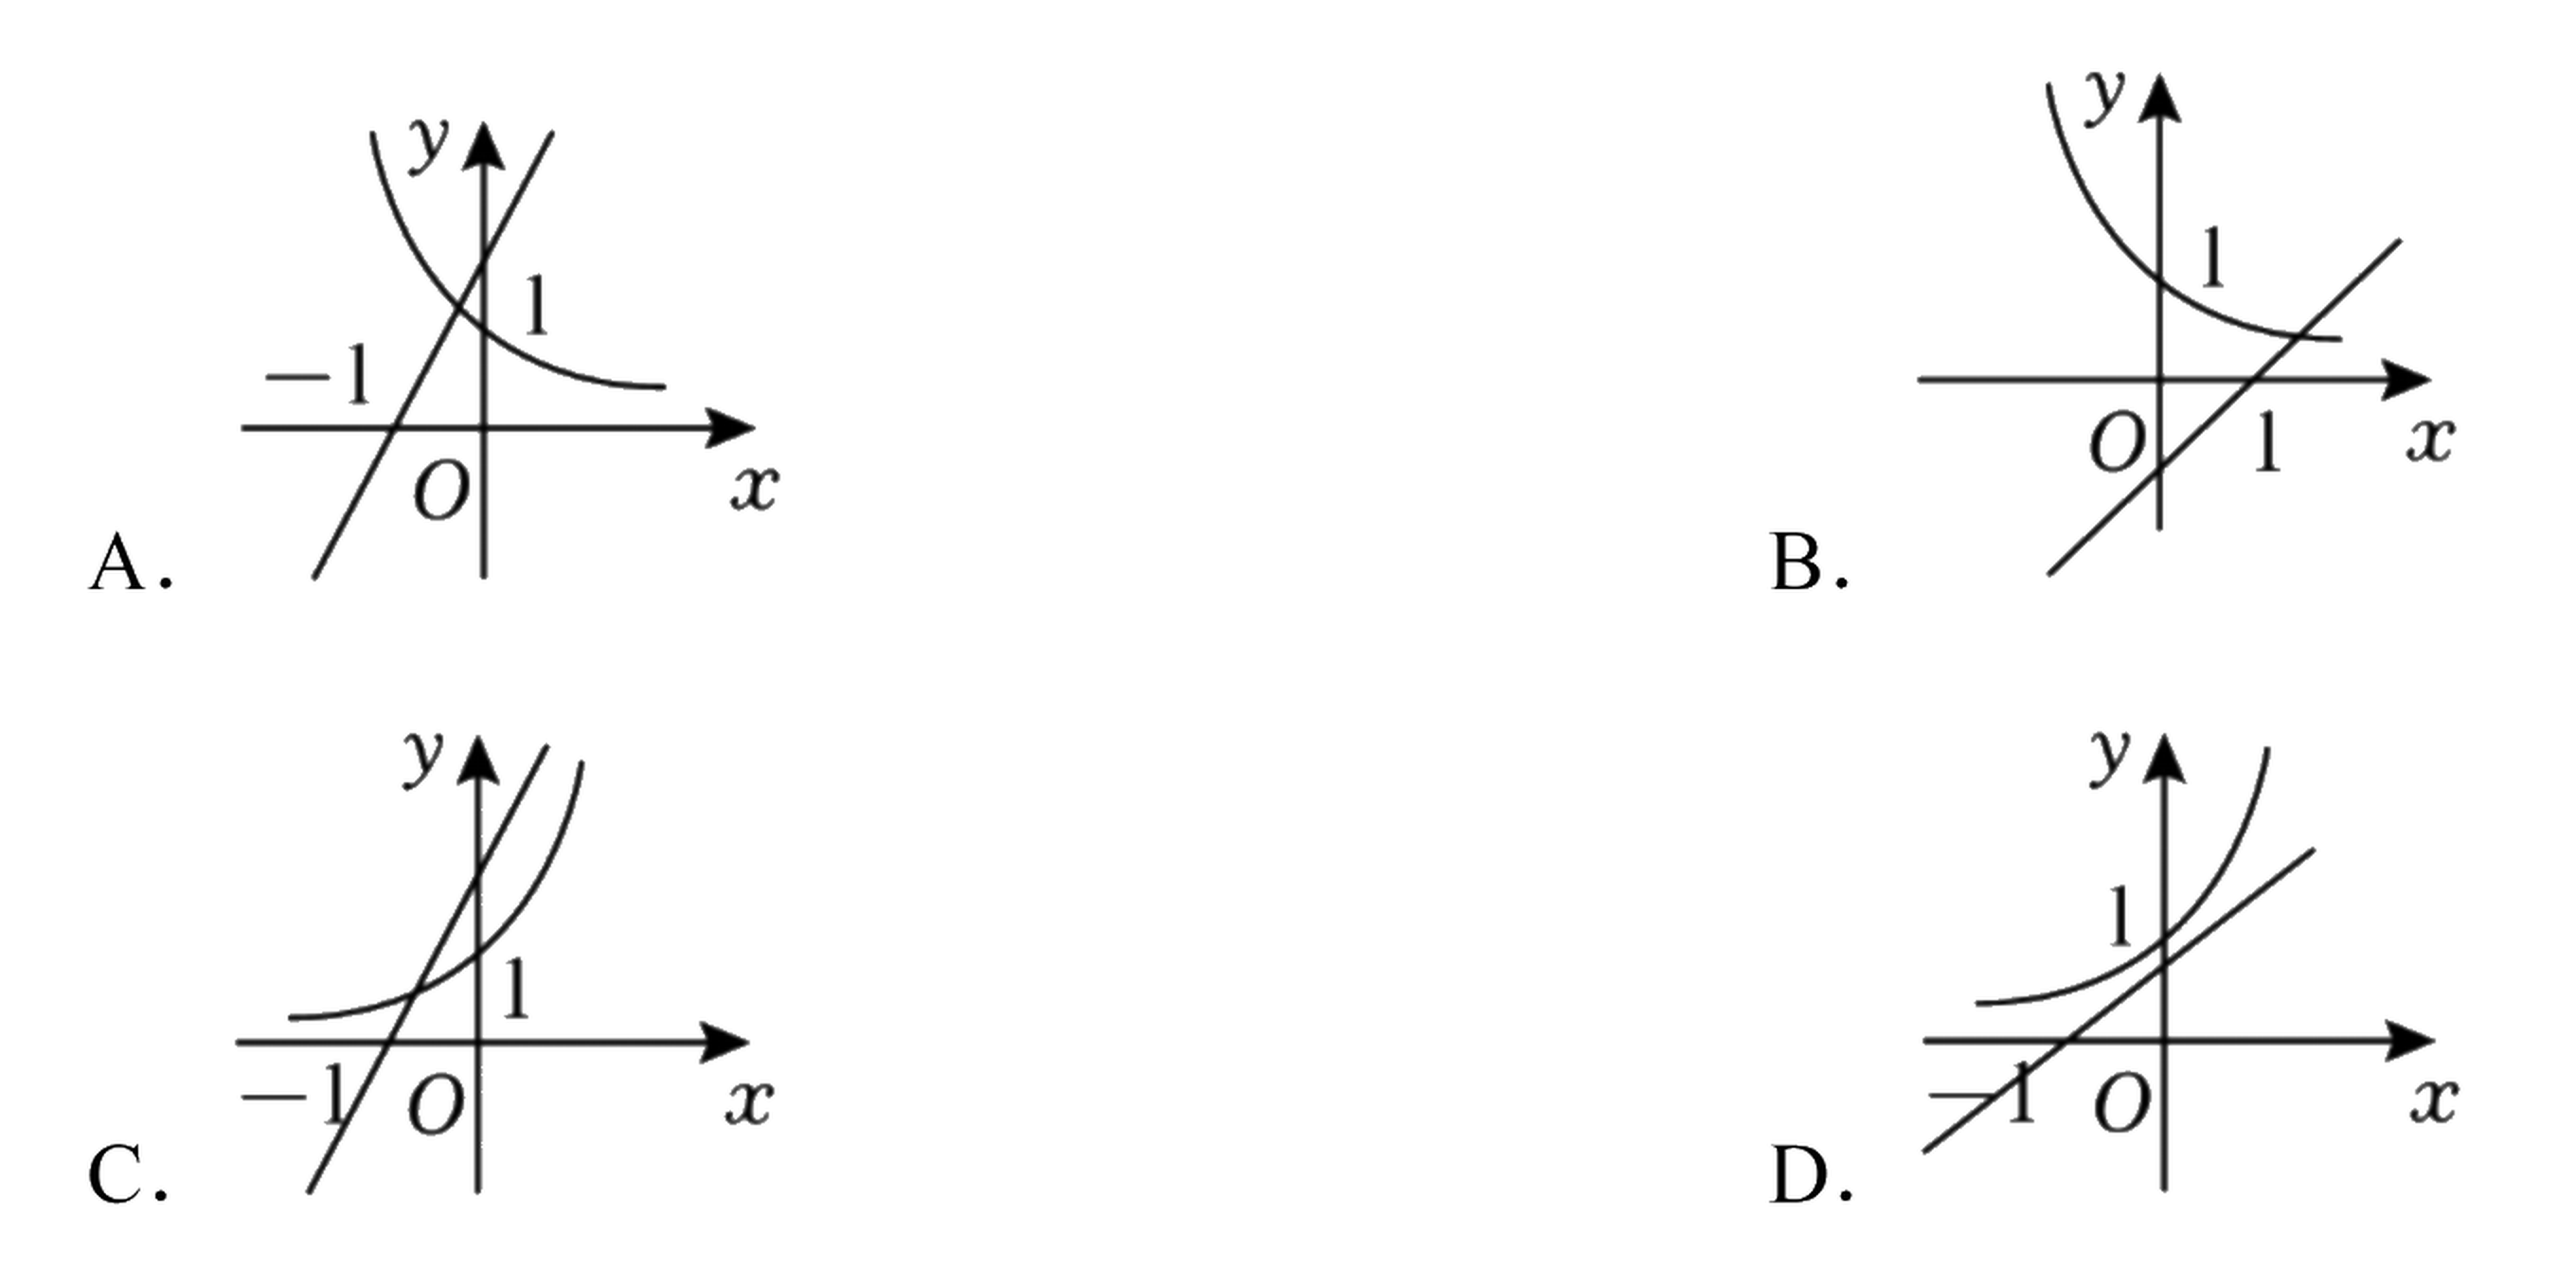
\includegraphics[width=0.80\textwidth]{figures/gao130_q15.png}
\end{center}

\ifanswer
\solbegin
\step{A 中，由指数函数 $y=a^x(a>0$ 且 $a\neq1)$ 图像递减得 $0<a<1$，}
\step{而一次函数 $y=a(x+1)$ 的图像与 $y$ 轴交点纵坐标为 $a>1$，二者矛盾，}
\step{所以 A 错；}
\step{由一次函数 $y=a(x+1)$ 的图像与 $x$ 轴交点横坐标为 $-1$，排除 B；}
\step{C 中，由指数函数 $y=a^x(a>0$ 且 $a\neq1)$ 图像递减得 $a>1$，}% 原卷"递减得 a>1"系笔误（应为"递增"），与 A 中"递减得 0<a<1"自相矛盾，照录
\step{而一次函数 $y=a(x+1)$ 的图像与 $y$ 轴交点纵坐标为 $a>1$，二者 $a$ 值吻合，}
\step{所以 C 对；}
\step{D 中，由一次函数 $y=a(x+1)$ 的图像得 $a=1$，与 $a>0$ 且 $a\neq1$ 矛盾，}
\step{所以 D 错.}
\step{故选 $C$.}
\solend
\fi

\item 设 $A_1$、$A_2$、$A_3$、$\cdots$、$A_7$ 是均含有 $2$ 个元素的集合，且 $A_1\cap A_7=\varnothing$，$A_i\cap A_{i+1}=\varnothing(i=1,2,3,\cdots,6)$，记 $B=A_1\cup A_2\cup A_3\cup\cdots\cup A_7$，则 $B$ 中元素个数的最小值是\mbox{（\quad）}

\keepwithprev
A. $4$\qquad B. $5$\qquad C. $6$\qquad D. $7$

\ifanswer
\solbegin
\step{取 $A_1=\{1,2\}$，$A_2=\{3,4\}$，$A_3=\{1,2\}$，$A_4=\{3,4\}$，$A_5=\{1,5\}$，$A_6=\{2,3\}$，$A_7=\{4,5\}$，}
\step{所以 $B$ 中元素个数的最小值是 $5$，故选 $B$.}
\solend
\fi

\end{enumerate}

\bigsec{三、解答题}

\begin{enumerate}
\setcounter{enumi}{16}

\item 已知全集为 $\R$，集合 $A=\{x\mid-2\leqslant x\leqslant5\}$，集合 $B=\{x\mid m-1\leqslant x\leqslant2m+1\}$．

(1) 求 $\overline{A}$；

(2) 若 $A\cup B=A$，求实数 $m$ 的取值范围．

\ifanswer
\solbegin
\step{(1) $(-\infty,-2)\cup(5,+\infty)$；}
\step{(2) 若 $A\cup B=A$，则 $B\subseteq A$，}
\step{当 $B=\varnothing$ 时，$m-1>2m+1$，解得 $m<-2$；}
\step{当 $B\neq\varnothing$ 时，$\begin{cases}m-1\leqslant2m+1\\m-1\geqslant-2\\2m+1\leqslant5\end{cases}$，解得 $-1\leqslant m\leqslant2$；}
\step{故实数 $m$ 的取值范围为 $\{m\mid-1\leqslant m\leqslant2$ 或 $m<-2\}$.}
\solend
\fi

\item 在不等式的应用中，有一些很基本而十分重要的不等式，如平均值不等式和三角不等式等，我们将其统称为基本不等式．

(1) 已知 $x$、$y$ 为正数，且 $2x+y=2$，求 $\dfrac1x+\dfrac2y$ 的最小值；

(2) 若关于 $x$ 的不等式 $\lvert x+1\rvert+\lvert2-x\rvert\geqslant a^2+a+1$ 对于一切实数 $x$ 都成立，求实数 $a$ 的取值范围．

\ifanswer
\solbegin
\step{(1) 因为 $x$、$y$ 为正数，且 $2x+y=2$，}
\step{所以 $\dfrac1x+\dfrac2y=\dfrac12\left(\dfrac1x+\dfrac2y\right)(2x+y)=\dfrac12\left(4+\dfrac yx+\dfrac{4x}y\right)\geqslant\dfrac12\left(4+2\sqrt{\dfrac yx\cdot\dfrac{4x}y}\right)=4$，}
\step{当且仅当 $\dfrac yx=\dfrac{4x}y$，即 $x=\dfrac12$，$y=1$ 时取等号，所以 $\dfrac1x+\dfrac2y$ 的最小值为 $4$；}
\step{(2) 由绝对值三角不等式得 $\lvert x+1\rvert+\lvert2-x\rvert\geqslant\lvert(x+1)+(2-x)\rvert=3$，}
\step{当且仅当 $-1\leqslant x\leqslant2$ 时取等号，所以 $\lvert x+1\rvert+\lvert2-x\rvert$ 的最小值为 $3$，}
\step{因为关于 $x$ 的不等式 $\lvert x+1\rvert+\lvert2-x\rvert\geqslant a^2+a+1$ 对于一切实数 $x$ 都成立，}
\step{所以 $a^2+a+1\leqslant3$，即 $a^2+a-2\leqslant0$，解得 $-2\leqslant a\leqslant1$，}
\step{所以实数 $a$ 的取值范围是 $[-2,1]$.}
\solend
\fi

\item 某医学专家为研究传染病传播中病毒细胞的发展规律，将病毒细胞注入一只小白鼠体内进行试验，经检测，病毒细胞的个数 $y$ 与天数 $x$ 的部分数据如表所示：

\begin{center}
\begin{tabular}{|c|c|c|c|c|c|c|c|}
\hline
天数 $(x)$ & $1$ & $2$ & $3$ & $4$ & $5$ & $6$ & $\cdots$ \\
\hline
病毒细胞的个数 $(y)$ & $1$ & $2$ & $4$ & $8$ & $16$ & $32$ & $\cdots$ \\
\hline
\end{tabular}
\end{center}

(1) 若病毒细胞的个数 $y$ 关于天数 $x$ 的变化规律可选用以下两个函数模型之一进行近似刻画：① $y=a\cdot b^x(a>0$，$b>0$，$b\neq1)$；② $y=a\cdot x^k(a\neq0)$．请结合表格中的数据，选择合适的函数模型，说明理由，并求出相应的函数表达式；

(2) 若该病毒细胞在小白鼠体内的个数超过 $10^8$，小白鼠将死亡，但注射某种药物，可杀死其体内 $98\%$ 的病毒细胞．则在 (1) 的条件下，为了使小白鼠在试验过程中不死亡，第一次最迟应在何时注射该种药物？（结果精确到天）

\ifanswer
\solbegin
\step{(1) 选择模型① $y=a\cdot b^x(a>0$，$b>0$，$b\neq1)$，理由如下：}
\step{观察表格数据，$y$ 的值随 $x$ 呈指数倍增：}
\step{$x=1$ 时，$y=1$，$x=2$ 时，$y=2$，$x=3$ 时，$y=4$，}
\step{后一天的病毒数是前一天的 $2$ 倍，符合指数增长的特征；}
\step{若选用幂函数模型 $y=a\cdot x^k$，代入前两组数据得 $a\cdot1^k=1$、$a\cdot2^k=2$，}
\step{解得 $a=1$，$k=1$，即 $y=x$，}
\step{但 $x=3$ 时，$y=3$ 与表格中 $y=4$ 严重不符，因此幂函数不匹配；}
\step{将 $(1,1)$ 代入 $y=a\cdot b^x$ 得 $a\cdot b=1$，}
\step{将 $(2,2)$ 代入得 $a\cdot b^2=2$，两式相除得 $b=2$，进而得 $a=\dfrac12$，}
\step{验证所有表格点均满足 $y=2^{x-1}$，最终函数表达式为 $y=2^{x-1}(x\in\N^*)$；}
\step{(2) 由题意得第一次注射药物前病毒细胞个数 $y$ 关于天数 $x(x\in\N^*)$ 的函数}
\step{关系式为 $y=2^{x-1}(x\in\N^*)$，}
\step{为了使小白鼠在试验过程中不死亡，则 $2^{x-1}\leqslant10^8$，}
\step{所以 $x-1\leqslant\log_210^8=8\log_210=\dfrac8{\lg2}$，解得 $x\leqslant1+\dfrac8{\lg2}\approx27.6$，}
\step{又 $x\in\N^*$，所以第一次最迟应在第 $27$ 天注射该种药物.}
\solend
\fi

\item 对在直角坐标系的第一象限内的任意两点 $(a,b)$，$(c,d)$ 作如下定义：$\dfrac ab>\dfrac cd$，那么称点 $(a,b)$ 是点 $(c,d)$ 的“上位点”，同时点 $(c,d)$ 是点 $(a,b)$ 的“下位点”．

(1) 试写出点 $(3,5)$ 的一个“上位点”坐标和一个“下位点”坐标；

(2) 设 $a$、$b$、$c$、$d$ 均为正数，且点 $(a,b)$ 是点 $(c,d)$ 的上位点，请判断点 $P(a+c,b+d)$ 是否既是点 $(a,b)$ 的“下位点”又是点 $(c,d)$ 的“上位点”，如果是，请证明；如果不是，请说明理由；

(3) 设正整数 $n$ 满足以下条件：对任意实数 $m\in\{t\mid0<t<4,t\in\Z\}$，总存在正整数 $k$，使得点 $(n,k)$ 既是点 $(4,m)$ 的“下位点”，又是点 $(5,m+1)$ 的“上位点”，求正整数 $n$ 的最小值．

\ifanswer
\solbegin
\step{(1) 由 $\dfrac34>\dfrac35>\dfrac36$ 得点 $(3,5)$ 的一个“上位点”的坐标为 $(3,4)$，}
\step{一个“下位点”的坐标为 $(3,6)$.}
\step{(2) 是，证明如下：}
\step{因为 $a$、$b$、$c$、$d$ 均为正数，点 $(a,b)$ 是点 $(c,d)$ 的“上位点”，}
\step{所以 $\dfrac ab>\dfrac cd$，所以 $ad>bc$，}
\step{因为 $\dfrac{a+c}{b+d}-\dfrac ab=\dfrac{b(a+c)-a(b+d)}{b(b+d)}=\dfrac{bc-ad}{b(b+d)}<0$，所以 $\dfrac{a+c}{b+d}<\dfrac ab$，}
\step{点 $P(a+c,b+d)$ 是点 $(a,b)$ 的“下位点”，}
\step{因为 $\dfrac{a+c}{b+d}-\dfrac cd=\dfrac{d(a+c)-c(b+d)}{d(b+d)}=\dfrac{ad-bc}{d(b+d)}>0$.}
\step{所以 $\dfrac{a+c}{b+d}>\dfrac cd$ 点 $P(a+c,b+d)$ 是点 $(c,d)$ 的“上位点”；}
\step{所以 $P(a+c,b+d)$ 既是点 $(a,b)$ 的“下位点”又是点 $(c,d)$ 的“上位点”；}
\step{(3) 由题意得 $m=1,2,3$，}
\step{由题意存在正整数 $k$：$\dfrac5{m+1}<\dfrac nk<\dfrac4m$，所以 $\begin{cases}\dfrac n4<k<\dfrac{2n}5(m=1)\\\dfrac n2<k<\dfrac{3n}5(m=2)\\\dfrac{3n}4<k<\dfrac{4n}5(m=3)\end{cases}$，}
\step{检验：$n=1,2,\cdots,8$ 不能同时找到整数 $k$，}
\step{$n=9$：$m=1$ 取 $k=3$，$m=2$ 取 $k=5$，$m=3$ 取 $k=7$，均满足，}
\step{所以正整数 $n$ 的最小值为 $9$.}
\solend
\fi

\end{enumerate}

\end{document}
"
%
% ① 原始材料：微信公众号"魔都数学加油站"文章，连载"27学年高一140"，原文标题
% "27学年高一140——2026-2027年上海市北郊高级中学高一上期中"；
% 原文链接：https://mp.weixin.qq.com/s/XBEYuTheiBoqu15dtLuD6A。
%   ★ 编号不一致说明：公众号连载号印"140"，与上一批已入库的"高一140 甘泉外国语"
%   （同一公众号另一篇文章、同为期中卷）撞号，系公众号笔误/重复。本仓库数字编号
%   02—143 中"高一130"一直空缺（连载 130 暂未见原文），故将本卷本地编号定为"高一130"、
%   填补该空缺，使数字编号连续（basename 全程为 高一130_北郊高级中学_期中）；
%   连载号 143 归正牌卷"上海中学 高一上期中"；本卷连载号仍印 140，见材料流转表。
%   卷面标题印"2026-2027 年北郊高级中学高一上期中"（卷面只有学校名、不含"上海市"、
%   不含任何期号/连载号），本稿照卷面录入；粉红色水印"魔都数学加油站"及页脚未录入。
% 正文为 9 张 PNG 页（01、04、05、06、09 为 2560x3620；02、03、07、08 为 4762x6735，
% 同一篇各页分辨率不同，逐页按各自分辨率放大核对），题目下印有【解析】，为讲评版。
% 题目、解析均据原图转录。
%
% 卷首标题：原卷印作"2026-2027 年北郊高级中学高一上期中"，年份区间按全稿惯例排
% en dash；原卷未印副标题，本卷为期中卷、跨集合与常用逻辑用语／不等式／函数三章，
% 按题目内容补出"集合与常用逻辑用语、不等式、函数"（与 125／126／128／129／131／132／133
% 同期中卷口径相同）。
%
% 题号体例：本卷共 18 题——一、填空题 3—12（10 题）、二、选择题 13—16（4 题）、
% 三、解答题 17—20（4 题）。三节分别 \setcounter{enumi}{2}／{12}／{16}。
% 原卷从第 3 题起、无第 1、2 题、**无第 21 题**（第 20 题解析续至 09 页，末行
% "所以正整数 n 的最小值为 9."，09 页下半页整片空白＋水印收尾、无第 10 页），本稿保留原题号。
%
% ② 与原卷的排版差异：
%   ① 原文从第 3 题起，本稿保留原题号；原卷止于第 20 题、无第 21 题、无附加题节；
%   ② 原卷每题下直接印【解析】，本稿按全稿惯例置于答案版；全卷 18 题均印【解析】、
%      无独立【答案】段，四道选择题答案在解析末句"故选 C／D／C／B"，括号
%      \mbox{（\quad）} 留空、不另提 \ans{}；全卷 0 处 \ans{}，答案版【解析】标记数 18＝题数；
%   ③ 原卷未印副标题，本稿按"知识模块"口径补出；
%   ④ 原卷填空横线按全稿惯例排为 \blankline[4.4em]；选择题括号排 \mbox{（\quad）}、
%      每个选项段前按惯例加 \keepwithprev；解答题不留作答区、不加 \anspace（讲评版）；
%   ⑤ 原卷数集排斜体 $R$／$N$，按全稿惯例改 \R／\N；空集记号 \varnothing；
%      绝对值排 \lvert…\rvert，集合描述竖线排 \mid；不等号按全稿惯例排 \leqslant／\geqslant；
%      补集照原卷上划线 \overline{A}；
%   ⑥ 1 幅插图 + 1 张印刷表格：第 15 题四幅坐标函数图象选项（04 页）取原卷截图
%      去粉色水印、去色、按原卷 2x2 排布合并为 figures/gao130_q15.png（非插图重绘），
%      放在 \keepwithprev 之后 \begin{center} 内、三版都出；第 19 题 (1) 印刷数据表格
%      （07 页，天数 x 1—6／病毒细胞个数 y 1/2/4/8/16/32）按原卷用 tabular 重排、
%      题干内三版都出（非插图）。
%      第 15 题是"二、选择题"节内带大图块的第三题（Q13 为节首题但无图），
%      在 \bigsec{二、选择题} 之前加 \needvspace{11cm} 连节标题一起量、Q15 \item 之前
%      加 \needvspace{9cm}——守卫必须放在 \bigsec 之前，放标题之后会让"二、选择题"
%      孤立在页末（B 类，照 高一26／40／59／136／140 成例）；三版切页审计均"合计异常：无"；
%   ⑦ 子题标号 (1)(2)(3) 原卷用半角括号，照录；圈数字 ①②③④ 照录；
%      数学式内半角逗号照录（如第 14 题 $(a>0,a\neq1)$、第 16 题
%      $(i=1,2,3,\cdots,6)$、第 20 题 $m=1,2,3$ 等）；
%      行末西文句点按全稿惯例照录；
%   ⑧ 题干中的中文弯引号按原卷照录（Q12"变项和"、Q20"上位点""下位点"等），
%      注释内一律 ASCII 引号；原卷"图像"用词逐处照录（Q9、Q15 均作"图像"）。
%
% ③ 行数复核：一条 \step = 原卷解析的一个印刷行（cases 块与 tabular 各作一个印刷行计）。
%   逐题 \step 条数，合计 98 条（Q3:3 Q4:2 Q5:2 Q6:1 Q7:1 Q8:3 Q9:5 Q10:10 Q11:6
%   Q12:7 Q13:1 Q14:2 Q15:10 Q16:2 Q17:5 Q18:8 Q19:15 Q20:15），与原卷印刷行逐题相等。
%
% ④ 判别式／子集符号结论：
%   判别式：全卷未出现判别式记号（无 $\Delta$、无 $\triangle$）；
%   子集符号：第 4 题题干"$B\subseteq A$"、第 4 题【解析】"$B\subseteq A$"、
%      第 17 题 (2)【解析】"$B\subseteq A$"三处原卷均印带下划线 $\subseteq$，逐处
%      放大核对、照录 \subseteq；全卷未出现单线 \subset。
%
% ⑤ 原卷存疑照录（均照录未改，正文对应处另有 % 注）：
%   ① 第 15 题【解析】"C 中，由指数函数 $y=a^x$ 图像递减得 $a>1$"——"递减"应为
%      "递增"之误（与同题 A 中"递减得 $0<a<1$"自相矛盾），原卷如此，照录并加注；
%   ② 第 16 题题干"$A_1\cap A_7=\varnothing$""$A_i\cap A_{i+1}=\varnothing$"
%      的空集记号与解析所列各集合逐处照录；
%   ③ 第 19 题 (2) 题干"可杀死其体内 98% 的病毒细胞"、解析 (2) 只按 $y=2^{x-1}$
%      与 $10^8$ 比较（未另计 98%），照录不补步。
%
% ⑥ 跨页续印按题合并：Q8 题干在 01 页末、解析在 02 页；Q9 题干在 02 页、
%   解析在 02 页；Q10 题干在 02 页、解析前 5 行在 02—03 页、后 5 行在 03 页；
%   Q12 题干跨 03 页、解析首 5 行在 03 页末、末行在 04 页；Q15 题干在 04 页、
%   四幅图与解析前段在 04 页、解析续在 05 页；Q17 解析跨 05—06 页；Q18 题干与
%   (1) 解析在 06 页、(2) 解析在 06—07 页；Q19 表格在 07 页、解析跨 07—08 页；
%   Q20 定义与三小问在 08 页、解析 (1)(2) 在 08—09 页、解析 (3) 在 09 页；
%   本稿按题连排，不丢行。
%
\documentclass[a4paper,11pt]{article}
\usepackage{common}

\begin{document}

\examtitlest[3]{2026--2027 年北郊高级中学高一上期中}{集合与常用逻辑用语、不等式、函数}

\bigsec{一、填空题}

\begin{enumerate}
\setcounter{enumi}{2}

\item 不等式 $\dfrac{x-3}{x+1}<2$ 的解集为\blankline[4.4em].

\ifanswer
\solbegin
\step{不等式 $\dfrac{x-3}{x+1}<2$ 可化为 $\dfrac{x-3}{x+1}-2<0$，即 $\dfrac{x-3-2(x+1)}{x+1}<0$，}
\step{化简为 $\dfrac{x+5}{x+1}>0$，解得 $x<-5$ 或 $x>-1$，}
\step{所以不等式的解集为 $\{x\mid x<-5$ 或 $x>-1\}$.}
\solend
\fi

\item 已知集合 $A=\{x\mid0<x<a\}$，$B=\{x\mid1<x<2\}$，若 $B\subseteq A$，则实数 $a$ 的取值范围为\blankline[4.4em].

\ifanswer
\solbegin
\step{已知集合 $A=\{x\mid0<x<a\}$，$B=\{x\mid1<x<2\}$，}
\step{若 $B\subseteq A$，则 $a\geqslant2$，所以实数 $a$ 的取值范围是 $\{a\mid a\geqslant2\}$.}
\solend
\fi

\item 已知关于 $x$ 的方程 $x^2+x+c=0$ 的两个实数根为 $x_1$、$x_2$，若 $x_1^2x_2+x_2^2x_1=3$，则实数 $c=$\blankline[4.4em].

\ifanswer
\solbegin
\step{由韦达定理得 $x_1+x_2=-1$，$x_1x_2=c$，所以 $x_1^2x_2+x_2^2x_1=(x_1+x_2)x_1x_2=-c=3$，}
\step{所以 $c=-3$.}
\solend
\fi

\item 已知 $10^x=3$，$10^y=64$，则 $10^{x-\frac y3}=$\blankline[4.4em].

\ifanswer
\solbegin
\step{$10^{x-\frac y3}=10^x\div\sqrt[3]{10^y}=\dfrac34$.}
\solend
\fi

\item 若 $\lg2=a$，则可用 $a$ 表示 $\log_280=$\blankline[4.4em].

\ifanswer
\solbegin
\step{$\log_280=\dfrac{\lg80}{\lg2}=\dfrac{\lg10+\lg8}{\lg2}=\dfrac{1+3\lg2}{\lg2}=\dfrac{1+3a}{a}$.}
\solend
\fi

\item 已知 $a+2b=1$，则 $3^a+9^b$ 的最小值为\blankline[4.4em].

\ifanswer
\solbegin
\step{因为 $a+2b=1$，所以 $3^a+9^b=3^a+3^{2b}\geqslant2\sqrt{3^a\cdot3^{2b}}=2\sqrt{3^{a+2b}}=2\sqrt3$，}
\step{当且仅当 $3^a=3^{2b}$，且 $a+2b=1$，即 $a=\dfrac12$，$b=\dfrac14$ 时取等号，}
\step{故最小值为 $2\sqrt3$.}
\solend
\fi

\item 下列函数的图像关于原点成中心对称，且在区间 $(0,+\infty)$ 上是严格增函数的是\blankline[4.4em]（请填写全部正确的序号）.

① $y=\sqrt{x}$；② $y=\sqrt[3]{x}$；③ $y=x^{\frac23}$；④ $y=x^{-\frac13}$.

\ifanswer
\solbegin
\step{① $y=\sqrt{x}$ 的定义域为 $[0,+\infty)$，故其图像不关于原点成中心对称，①错误；}
\step{② $y=\sqrt[3]{x}$ 是奇函数，且在区间 $(0,+\infty)$ 上是严格增函数，②正确；}
\step{③ $y=x^{\frac23}$ 是偶函数，其图像关于 $y$ 轴对称，不关于原点成中心对称，③错误；}
\step{④由于幂指数 $-\dfrac13<0$，故 $y=x^{-\frac13}$ 在区间 $(0,+\infty)$ 上是严格减函数，④错误.}
\step{故正确的是②.}
\solend
\fi

\item 设 $a>0$ 且 $a\neq1$，若函数 $y=a^{2x}+2a^x-3$ 在区间 $[-1,1]$ 上的最大值为 $21$，则实数 $a$ 的值为\blankline[4.4em].

\ifanswer
\solbegin
\step{令 $t=a^x$，$x\in[-1,1]$，}
\step{当 $a>1$ 时，$t=a^x$ 严格增，则 $t\in\left[\dfrac1a,a\right]$，}
\step{则函数 $y=t^2+2t-3$，对称轴为 $t=-1$，}
\step{所以函数 $y=t^2+2t-3$ 在 $\left[\dfrac1a,a\right]$ 上严格增，}
\step{所以当 $t=a$ 时，$y$ 取得最大值 $a^2+2a-3=21$，解得 $a=4$ 或 $-6$（舍去）；}
\step{当 $0<a<1$ 时，$t=a^x$ 严格减，则 $t\in\left[a,\dfrac1a\right]$，}
\step{则函数 $y=t^2+2t-3$，对称轴为 $t=-1$，}
\step{所以函数 $y=t^2+2t-3$ 在 $\left[a,\dfrac1a\right]$ 上严格增，}
\step{所以当 $t=\dfrac1a$ 时，$y$ 取得最大值 $\dfrac1{a^2}+\dfrac2a-3=21$，解得 $a=\dfrac14$ 或 $-\dfrac16$（舍去）；}
\step{综上所述，实数 $a$ 的值为 $4$ 或 $\dfrac14$.}
\solend
\fi

\item 在关于 $x$ 的不等式 $x^2+(m+1)x+m<0$ 的解集中恰有两个整数，则实数 $m$ 的取值范围是\blankline[4.4em].

\ifanswer
\solbegin
\step{关于 $x$ 的不等式 $x^2+(m+1)x+m<0$ 可化为 $(x+1)(x+m)<0$，}
\step{当 $m>1$ 时，$-m<-1$，解不等式得 $-m<x<-1$；}
\step{当 $m<1$ 时，$-m>-1$，解不等式得 $-1<x<-m$；}
\step{由不等式的解集中恰有两个整数，}
\step{则 $-4\leqslant-m<-3$ 或 $1<-m\leqslant2$，即 $3<m\leqslant4$ 或 $-2\leqslant m<-1$，}
\step{所以 $m$ 的取值范围是 $[-2,-1)\cup(3,4]$.}
\solend
\fi

\item 已知集合 $M$ 的元素均为正整数，定义集合 $M$ 的“变项和”为：将 $M$ 中每个元素 $m$ 都乘以 $(-1)^m$ 后再求和．若集合 $A=\{n\mid1\leqslant n\leqslant20,n\in\N\}$，则集合 $A$ 的所有非空子集的“变项和”的总和为\blankline[4.4em].

\ifanswer
\solbegin
\step{集合 $A=\{n\mid1\leqslant n\leqslant20,n\in\N\}$ 中一共有 $20$ 个元素，}
\step{固定选中 $k$，剩下 $19$ 个元素任选，共 $2^{19}$ 个子集包含 $k$，每个 $k$ 贡献 $(-1)^k\cdot k\cdot2^{19}$，}
\step{$A=\{1,2,\cdots,20\}$，}
\step{奇数 $k=1,3,\cdots,19$，共 $10$ 个，$(-1)^k\cdot k=-k$，}
\step{偶数 $k=2,4,\cdots,20$，共 $10$ 个，$(-1)^k\cdot k=k$，}
\step{所以集合 $A$ 的所有非空子集的“变项和”的总和}
\step{为 $S=2^{19}\times[(-1+2)+(-3+4)+\cdots+(-19+20)]=2^{19}\times10=524880$.}
\solend
\fi

\end{enumerate}

% 第 15 题四幅图是"二、选择题"节内大图块；守卫须放在 \bigsec 之前连节标题一起量，
% 否则"二、选择题"会孤立在页末（B 类，照 高一26／40／59／136／140 成例）
\needvspace{11cm}
\bigsec{二、选择题}

\begin{enumerate}
\setcounter{enumi}{12}

\item 设 $ab>0$，则“$a>b$”是“$\dfrac1a<\dfrac1b$”的\mbox{（\quad）}

\keepwithprev
A. 充分非必要条件\qquad B. 必要非充分条件

C. 充要条件\qquad D. 既非充分也非必要条件

\ifanswer
\solbegin
\step{因为 $ab>0$，所以 $a>b\Leftrightarrow\dfrac1a<\dfrac1b$，故选 $C$.}
\solend
\fi

\item 已知 $A=\log_ax$，$B=\log_ay(a>0,a\neq1)$，则 $\log_a\dfrac{x^2}{\sqrt y}=$\mbox{（\quad）}

\keepwithprev
A. $\dfrac{A^2}{\sqrt B}$\qquad B. $2A^2B$\qquad C. $4AB$\qquad D. $2A-\dfrac12B$

\ifanswer
\solbegin
\step{由已知得 $x=a^A$，$y=a^B$，}
\step{所以 $\log_a\dfrac{x^2}{\sqrt y}=\log_a\dfrac{(a^A)^2}{\sqrt{a^B}}=\log_a\dfrac{a^{2A}}{a^{\frac12B}}=\log_a a^{2A-\frac12B}=2A-\dfrac12B$. 故选 $D$.}
\solend
\fi

% 第 15 题四幅坐标函数图象选项是一整块，守卫放在 \item 之前
\needvspace{9cm}
\item 在同一平面直角坐标系中，指数函数 $y=a^x(a>0$ 且 $a\neq1)$ 和一次函数 $y=a(x+1)$ 的图像关系可能是\mbox{（\quad）}

\keepwithprev
\begin{center}
% 四幅坐标函数图象选项取原卷 04 页截图去粉色水印、去色，按原卷 2x2 排布合并为一张
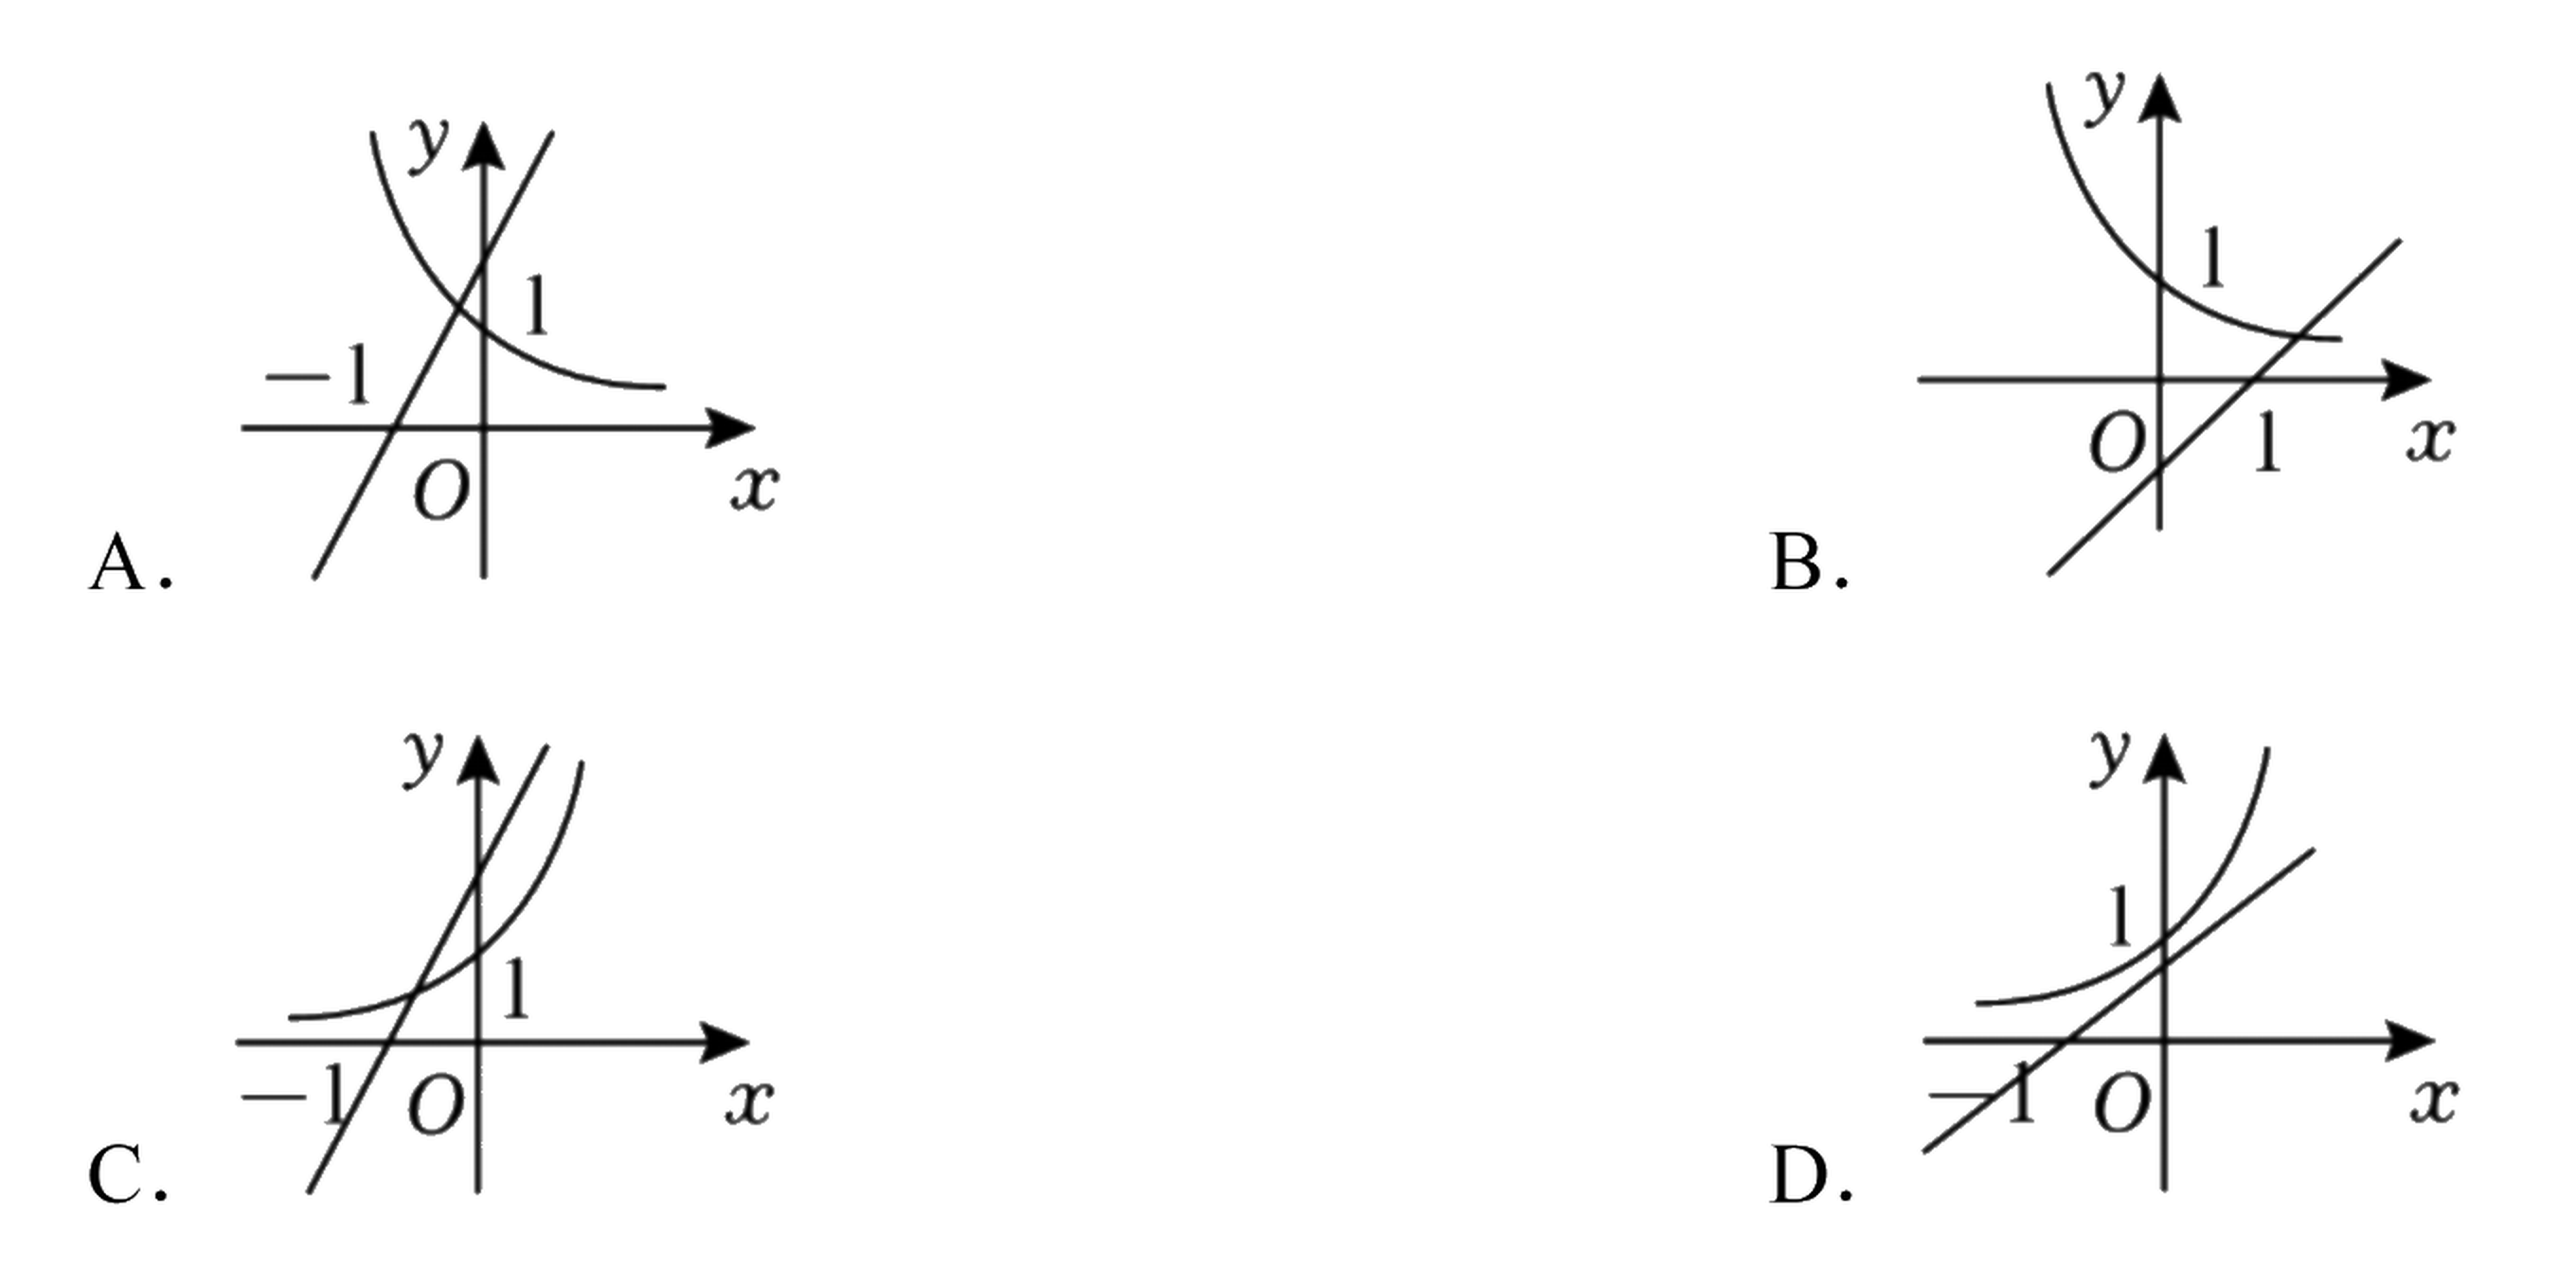
\includegraphics[width=0.80\textwidth]{figures/gao130_q15.png}
\end{center}

\ifanswer
\solbegin
\step{A 中，由指数函数 $y=a^x(a>0$ 且 $a\neq1)$ 图像递减得 $0<a<1$，}
\step{而一次函数 $y=a(x+1)$ 的图像与 $y$ 轴交点纵坐标为 $a>1$，二者矛盾，}
\step{所以 A 错；}
\step{由一次函数 $y=a(x+1)$ 的图像与 $x$ 轴交点横坐标为 $-1$，排除 B；}
\step{C 中，由指数函数 $y=a^x(a>0$ 且 $a\neq1)$ 图像递减得 $a>1$，}% 原卷"递减得 a>1"系笔误（应为"递增"），与 A 中"递减得 0<a<1"自相矛盾，照录
\step{而一次函数 $y=a(x+1)$ 的图像与 $y$ 轴交点纵坐标为 $a>1$，二者 $a$ 值吻合，}
\step{所以 C 对；}
\step{D 中，由一次函数 $y=a(x+1)$ 的图像得 $a=1$，与 $a>0$ 且 $a\neq1$ 矛盾，}
\step{所以 D 错.}
\step{故选 $C$.}
\solend
\fi

\item 设 $A_1$、$A_2$、$A_3$、$\cdots$、$A_7$ 是均含有 $2$ 个元素的集合，且 $A_1\cap A_7=\varnothing$，$A_i\cap A_{i+1}=\varnothing(i=1,2,3,\cdots,6)$，记 $B=A_1\cup A_2\cup A_3\cup\cdots\cup A_7$，则 $B$ 中元素个数的最小值是\mbox{（\quad）}

\keepwithprev
A. $4$\qquad B. $5$\qquad C. $6$\qquad D. $7$

\ifanswer
\solbegin
\step{取 $A_1=\{1,2\}$，$A_2=\{3,4\}$，$A_3=\{1,2\}$，$A_4=\{3,4\}$，$A_5=\{1,5\}$，$A_6=\{2,3\}$，$A_7=\{4,5\}$，}
\step{所以 $B$ 中元素个数的最小值是 $5$，故选 $B$.}
\solend
\fi

\end{enumerate}

\bigsec{三、解答题}

\begin{enumerate}
\setcounter{enumi}{16}

\item 已知全集为 $\R$，集合 $A=\{x\mid-2\leqslant x\leqslant5\}$，集合 $B=\{x\mid m-1\leqslant x\leqslant2m+1\}$．

(1) 求 $\overline{A}$；

(2) 若 $A\cup B=A$，求实数 $m$ 的取值范围．

\ifanswer
\solbegin
\step{(1) $(-\infty,-2)\cup(5,+\infty)$；}
\step{(2) 若 $A\cup B=A$，则 $B\subseteq A$，}
\step{当 $B=\varnothing$ 时，$m-1>2m+1$，解得 $m<-2$；}
\step{当 $B\neq\varnothing$ 时，$\begin{cases}m-1\leqslant2m+1\\m-1\geqslant-2\\2m+1\leqslant5\end{cases}$，解得 $-1\leqslant m\leqslant2$；}
\step{故实数 $m$ 的取值范围为 $\{m\mid-1\leqslant m\leqslant2$ 或 $m<-2\}$.}
\solend
\fi

\item 在不等式的应用中，有一些很基本而十分重要的不等式，如平均值不等式和三角不等式等，我们将其统称为基本不等式．

(1) 已知 $x$、$y$ 为正数，且 $2x+y=2$，求 $\dfrac1x+\dfrac2y$ 的最小值；

(2) 若关于 $x$ 的不等式 $\lvert x+1\rvert+\lvert2-x\rvert\geqslant a^2+a+1$ 对于一切实数 $x$ 都成立，求实数 $a$ 的取值范围．

\ifanswer
\solbegin
\step{(1) 因为 $x$、$y$ 为正数，且 $2x+y=2$，}
\step{所以 $\dfrac1x+\dfrac2y=\dfrac12\left(\dfrac1x+\dfrac2y\right)(2x+y)=\dfrac12\left(4+\dfrac yx+\dfrac{4x}y\right)\geqslant\dfrac12\left(4+2\sqrt{\dfrac yx\cdot\dfrac{4x}y}\right)=4$，}
\step{当且仅当 $\dfrac yx=\dfrac{4x}y$，即 $x=\dfrac12$，$y=1$ 时取等号，所以 $\dfrac1x+\dfrac2y$ 的最小值为 $4$；}
\step{(2) 由绝对值三角不等式得 $\lvert x+1\rvert+\lvert2-x\rvert\geqslant\lvert(x+1)+(2-x)\rvert=3$，}
\step{当且仅当 $-1\leqslant x\leqslant2$ 时取等号，所以 $\lvert x+1\rvert+\lvert2-x\rvert$ 的最小值为 $3$，}
\step{因为关于 $x$ 的不等式 $\lvert x+1\rvert+\lvert2-x\rvert\geqslant a^2+a+1$ 对于一切实数 $x$ 都成立，}
\step{所以 $a^2+a+1\leqslant3$，即 $a^2+a-2\leqslant0$，解得 $-2\leqslant a\leqslant1$，}
\step{所以实数 $a$ 的取值范围是 $[-2,1]$.}
\solend
\fi

\item 某医学专家为研究传染病传播中病毒细胞的发展规律，将病毒细胞注入一只小白鼠体内进行试验，经检测，病毒细胞的个数 $y$ 与天数 $x$ 的部分数据如表所示：

\begin{center}
\begin{tabular}{|c|c|c|c|c|c|c|c|}
\hline
天数 $(x)$ & $1$ & $2$ & $3$ & $4$ & $5$ & $6$ & $\cdots$ \\
\hline
病毒细胞的个数 $(y)$ & $1$ & $2$ & $4$ & $8$ & $16$ & $32$ & $\cdots$ \\
\hline
\end{tabular}
\end{center}

(1) 若病毒细胞的个数 $y$ 关于天数 $x$ 的变化规律可选用以下两个函数模型之一进行近似刻画：① $y=a\cdot b^x(a>0$，$b>0$，$b\neq1)$；② $y=a\cdot x^k(a\neq0)$．请结合表格中的数据，选择合适的函数模型，说明理由，并求出相应的函数表达式；

(2) 若该病毒细胞在小白鼠体内的个数超过 $10^8$，小白鼠将死亡，但注射某种药物，可杀死其体内 $98\%$ 的病毒细胞．则在 (1) 的条件下，为了使小白鼠在试验过程中不死亡，第一次最迟应在何时注射该种药物？（结果精确到天）

\ifanswer
\solbegin
\step{(1) 选择模型① $y=a\cdot b^x(a>0$，$b>0$，$b\neq1)$，理由如下：}
\step{观察表格数据，$y$ 的值随 $x$ 呈指数倍增：}
\step{$x=1$ 时，$y=1$，$x=2$ 时，$y=2$，$x=3$ 时，$y=4$，}
\step{后一天的病毒数是前一天的 $2$ 倍，符合指数增长的特征；}
\step{若选用幂函数模型 $y=a\cdot x^k$，代入前两组数据得 $a\cdot1^k=1$、$a\cdot2^k=2$，}
\step{解得 $a=1$，$k=1$，即 $y=x$，}
\step{但 $x=3$ 时，$y=3$ 与表格中 $y=4$ 严重不符，因此幂函数不匹配；}
\step{将 $(1,1)$ 代入 $y=a\cdot b^x$ 得 $a\cdot b=1$，}
\step{将 $(2,2)$ 代入得 $a\cdot b^2=2$，两式相除得 $b=2$，进而得 $a=\dfrac12$，}
\step{验证所有表格点均满足 $y=2^{x-1}$，最终函数表达式为 $y=2^{x-1}(x\in\N^*)$；}
\step{(2) 由题意得第一次注射药物前病毒细胞个数 $y$ 关于天数 $x(x\in\N^*)$ 的函数}
\step{关系式为 $y=2^{x-1}(x\in\N^*)$，}
\step{为了使小白鼠在试验过程中不死亡，则 $2^{x-1}\leqslant10^8$，}
\step{所以 $x-1\leqslant\log_210^8=8\log_210=\dfrac8{\lg2}$，解得 $x\leqslant1+\dfrac8{\lg2}\approx27.6$，}
\step{又 $x\in\N^*$，所以第一次最迟应在第 $27$ 天注射该种药物.}
\solend
\fi

\item 对在直角坐标系的第一象限内的任意两点 $(a,b)$，$(c,d)$ 作如下定义：$\dfrac ab>\dfrac cd$，那么称点 $(a,b)$ 是点 $(c,d)$ 的“上位点”，同时点 $(c,d)$ 是点 $(a,b)$ 的“下位点”．

(1) 试写出点 $(3,5)$ 的一个“上位点”坐标和一个“下位点”坐标；

(2) 设 $a$、$b$、$c$、$d$ 均为正数，且点 $(a,b)$ 是点 $(c,d)$ 的上位点，请判断点 $P(a+c,b+d)$ 是否既是点 $(a,b)$ 的“下位点”又是点 $(c,d)$ 的“上位点”，如果是，请证明；如果不是，请说明理由；

(3) 设正整数 $n$ 满足以下条件：对任意实数 $m\in\{t\mid0<t<4,t\in\Z\}$，总存在正整数 $k$，使得点 $(n,k)$ 既是点 $(4,m)$ 的“下位点”，又是点 $(5,m+1)$ 的“上位点”，求正整数 $n$ 的最小值．

\ifanswer
\solbegin
\step{(1) 由 $\dfrac34>\dfrac35>\dfrac36$ 得点 $(3,5)$ 的一个“上位点”的坐标为 $(3,4)$，}
\step{一个“下位点”的坐标为 $(3,6)$.}
\step{(2) 是，证明如下：}
\step{因为 $a$、$b$、$c$、$d$ 均为正数，点 $(a,b)$ 是点 $(c,d)$ 的“上位点”，}
\step{所以 $\dfrac ab>\dfrac cd$，所以 $ad>bc$，}
\step{因为 $\dfrac{a+c}{b+d}-\dfrac ab=\dfrac{b(a+c)-a(b+d)}{b(b+d)}=\dfrac{bc-ad}{b(b+d)}<0$，所以 $\dfrac{a+c}{b+d}<\dfrac ab$，}
\step{点 $P(a+c,b+d)$ 是点 $(a,b)$ 的“下位点”，}
\step{因为 $\dfrac{a+c}{b+d}-\dfrac cd=\dfrac{d(a+c)-c(b+d)}{d(b+d)}=\dfrac{ad-bc}{d(b+d)}>0$.}
\step{所以 $\dfrac{a+c}{b+d}>\dfrac cd$ 点 $P(a+c,b+d)$ 是点 $(c,d)$ 的“上位点”；}
\step{所以 $P(a+c,b+d)$ 既是点 $(a,b)$ 的“下位点”又是点 $(c,d)$ 的“上位点”；}
\step{(3) 由题意得 $m=1,2,3$，}
\step{由题意存在正整数 $k$：$\dfrac5{m+1}<\dfrac nk<\dfrac4m$，所以 $\begin{cases}\dfrac n4<k<\dfrac{2n}5(m=1)\\\dfrac n2<k<\dfrac{3n}5(m=2)\\\dfrac{3n}4<k<\dfrac{4n}5(m=3)\end{cases}$，}
\step{检验：$n=1,2,\cdots,8$ 不能同时找到整数 $k$，}
\step{$n=9$：$m=1$ 取 $k=3$，$m=2$ 取 $k=5$，$m=3$ 取 $k=7$，均满足，}
\step{所以正整数 $n$ 的最小值为 $9$.}
\solend
\fi

\end{enumerate}

\end{document}
"
%
% ① 原始材料：微信公众号"魔都数学加油站"文章，连载"27学年高一140"，原文标题
% "27学年高一140——2026-2027年上海市北郊高级中学高一上期中"；
% 原文链接：https://mp.weixin.qq.com/s/XBEYuTheiBoqu15dtLuD6A。
%   ★ 编号不一致说明：公众号连载号印"140"，与上一批已入库的"高一140 甘泉外国语"
%   （同一公众号另一篇文章、同为期中卷）撞号，系公众号笔误/重复。本仓库数字编号
%   02—143 中"高一130"一直空缺（连载 130 暂未见原文），故将本卷本地编号定为"高一130"、
%   填补该空缺，使数字编号连续（basename 全程为 高一130_北郊高级中学_期中）；
%   连载号 143 归正牌卷"上海中学 高一上期中"；本卷连载号仍印 140，见材料流转表。
%   卷面标题印"2026-2027 年北郊高级中学高一上期中"（卷面只有学校名、不含"上海市"、
%   不含任何期号/连载号），本稿照卷面录入；粉红色水印"魔都数学加油站"及页脚未录入。
% 正文为 9 张 PNG 页（01、04、05、06、09 为 2560x3620；02、03、07、08 为 4762x6735，
% 同一篇各页分辨率不同，逐页按各自分辨率放大核对），题目下印有【解析】，为讲评版。
% 题目、解析均据原图转录。
%
% 卷首标题：原卷印作"2026-2027 年北郊高级中学高一上期中"，年份区间按全稿惯例排
% en dash；原卷未印副标题，本卷为期中卷、跨集合与常用逻辑用语／不等式／函数三章，
% 按题目内容补出"集合与常用逻辑用语、不等式、函数"（与 125／126／128／129／131／132／133
% 同期中卷口径相同）。
%
% 题号体例：本卷共 18 题——一、填空题 3—12（10 题）、二、选择题 13—16（4 题）、
% 三、解答题 17—20（4 题）。三节分别 \setcounter{enumi}{2}／{12}／{16}。
% 原卷从第 3 题起、无第 1、2 题、**无第 21 题**（第 20 题解析续至 09 页，末行
% "所以正整数 n 的最小值为 9."，09 页下半页整片空白＋水印收尾、无第 10 页），本稿保留原题号。
%
% ② 与原卷的排版差异：
%   ① 原文从第 3 题起，本稿保留原题号；原卷止于第 20 题、无第 21 题、无附加题节；
%   ② 原卷每题下直接印【解析】，本稿按全稿惯例置于答案版；全卷 18 题均印【解析】、
%      无独立【答案】段，四道选择题答案在解析末句"故选 C／D／C／B"，括号
%      \mbox{（\quad）} 留空、不另提 \ans{}；全卷 0 处 \ans{}，答案版【解析】标记数 18＝题数；
%   ③ 原卷未印副标题，本稿按"知识模块"口径补出；
%   ④ 原卷填空横线按全稿惯例排为 \blankline[4.4em]；选择题括号排 \mbox{（\quad）}、
%      每个选项段前按惯例加 \keepwithprev；解答题不留作答区、不加 \anspace（讲评版）；
%   ⑤ 原卷数集排斜体 $R$／$N$，按全稿惯例改 \R／\N；空集记号 \varnothing；
%      绝对值排 \lvert…\rvert，集合描述竖线排 \mid；不等号按全稿惯例排 \leqslant／\geqslant；
%      补集照原卷上划线 \overline{A}；
%   ⑥ 1 幅插图 + 1 张印刷表格：第 15 题四幅坐标函数图象选项（04 页）取原卷截图
%      去粉色水印、去色、按原卷 2x2 排布合并为 figures/gao130_q15.png（非插图重绘），
%      放在 \keepwithprev 之后 \begin{center} 内、三版都出；第 19 题 (1) 印刷数据表格
%      （07 页，天数 x 1—6／病毒细胞个数 y 1/2/4/8/16/32）按原卷用 tabular 重排、
%      题干内三版都出（非插图）。
%      第 15 题是"二、选择题"节内带大图块的第三题（Q13 为节首题但无图），
%      在 \bigsec{二、选择题} 之前加 \needvspace{11cm} 连节标题一起量、Q15 \item 之前
%      加 \needvspace{9cm}——守卫必须放在 \bigsec 之前，放标题之后会让"二、选择题"
%      孤立在页末（B 类，照 高一26／40／59／136／140 成例）；三版切页审计均"合计异常：无"；
%   ⑦ 子题标号 (1)(2)(3) 原卷用半角括号，照录；圈数字 ①②③④ 照录；
%      数学式内半角逗号照录（如第 14 题 $(a>0,a\neq1)$、第 16 题
%      $(i=1,2,3,\cdots,6)$、第 20 题 $m=1,2,3$ 等）；
%      行末西文句点按全稿惯例照录；
%   ⑧ 题干中的中文弯引号按原卷照录（Q12"变项和"、Q20"上位点""下位点"等），
%      注释内一律 ASCII 引号；原卷"图像"用词逐处照录（Q9、Q15 均作"图像"）。
%
% ③ 行数复核：一条 \step = 原卷解析的一个印刷行（cases 块与 tabular 各作一个印刷行计）。
%   逐题 \step 条数，合计 98 条（Q3:3 Q4:2 Q5:2 Q6:1 Q7:1 Q8:3 Q9:5 Q10:10 Q11:6
%   Q12:7 Q13:1 Q14:2 Q15:10 Q16:2 Q17:5 Q18:8 Q19:15 Q20:15），与原卷印刷行逐题相等。
%
% ④ 判别式／子集符号结论：
%   判别式：全卷未出现判别式记号（无 $\Delta$、无 $\triangle$）；
%   子集符号：第 4 题题干"$B\subseteq A$"、第 4 题【解析】"$B\subseteq A$"、
%      第 17 题 (2)【解析】"$B\subseteq A$"三处原卷均印带下划线 $\subseteq$，逐处
%      放大核对、照录 \subseteq；全卷未出现单线 \subset。
%
% ⑤ 原卷存疑照录（均照录未改，正文对应处另有 % 注）：
%   ① 第 15 题【解析】"C 中，由指数函数 $y=a^x$ 图像递减得 $a>1$"——"递减"应为
%      "递增"之误（与同题 A 中"递减得 $0<a<1$"自相矛盾），原卷如此，照录并加注；
%   ② 第 16 题题干"$A_1\cap A_7=\varnothing$""$A_i\cap A_{i+1}=\varnothing$"
%      的空集记号与解析所列各集合逐处照录；
%   ③ 第 19 题 (2) 题干"可杀死其体内 98% 的病毒细胞"、解析 (2) 只按 $y=2^{x-1}$
%      与 $10^8$ 比较（未另计 98%），照录不补步。
%
% ⑥ 跨页续印按题合并：Q8 题干在 01 页末、解析在 02 页；Q9 题干在 02 页、
%   解析在 02 页；Q10 题干在 02 页、解析前 5 行在 02—03 页、后 5 行在 03 页；
%   Q12 题干跨 03 页、解析首 5 行在 03 页末、末行在 04 页；Q15 题干在 04 页、
%   四幅图与解析前段在 04 页、解析续在 05 页；Q17 解析跨 05—06 页；Q18 题干与
%   (1) 解析在 06 页、(2) 解析在 06—07 页；Q19 表格在 07 页、解析跨 07—08 页；
%   Q20 定义与三小问在 08 页、解析 (1)(2) 在 08—09 页、解析 (3) 在 09 页；
%   本稿按题连排，不丢行。
%
\documentclass[a4paper,11pt]{article}
\usepackage{common}

\begin{document}

\examtitlest[3]{2026--2027 年北郊高级中学高一上期中}{集合与常用逻辑用语、不等式、函数}

\bigsec{一、填空题}

\begin{enumerate}
\setcounter{enumi}{2}

\item 不等式 $\dfrac{x-3}{x+1}<2$ 的解集为\blankline[4.4em].

\ifanswer
\solbegin
\step{不等式 $\dfrac{x-3}{x+1}<2$ 可化为 $\dfrac{x-3}{x+1}-2<0$，即 $\dfrac{x-3-2(x+1)}{x+1}<0$，}
\step{化简为 $\dfrac{x+5}{x+1}>0$，解得 $x<-5$ 或 $x>-1$，}
\step{所以不等式的解集为 $\{x\mid x<-5$ 或 $x>-1\}$.}
\solend
\fi

\item 已知集合 $A=\{x\mid0<x<a\}$，$B=\{x\mid1<x<2\}$，若 $B\subseteq A$，则实数 $a$ 的取值范围为\blankline[4.4em].

\ifanswer
\solbegin
\step{已知集合 $A=\{x\mid0<x<a\}$，$B=\{x\mid1<x<2\}$，}
\step{若 $B\subseteq A$，则 $a\geqslant2$，所以实数 $a$ 的取值范围是 $\{a\mid a\geqslant2\}$.}
\solend
\fi

\item 已知关于 $x$ 的方程 $x^2+x+c=0$ 的两个实数根为 $x_1$、$x_2$，若 $x_1^2x_2+x_2^2x_1=3$，则实数 $c=$\blankline[4.4em].

\ifanswer
\solbegin
\step{由韦达定理得 $x_1+x_2=-1$，$x_1x_2=c$，所以 $x_1^2x_2+x_2^2x_1=(x_1+x_2)x_1x_2=-c=3$，}
\step{所以 $c=-3$.}
\solend
\fi

\item 已知 $10^x=3$，$10^y=64$，则 $10^{x-\frac y3}=$\blankline[4.4em].

\ifanswer
\solbegin
\step{$10^{x-\frac y3}=10^x\div\sqrt[3]{10^y}=\dfrac34$.}
\solend
\fi

\item 若 $\lg2=a$，则可用 $a$ 表示 $\log_280=$\blankline[4.4em].

\ifanswer
\solbegin
\step{$\log_280=\dfrac{\lg80}{\lg2}=\dfrac{\lg10+\lg8}{\lg2}=\dfrac{1+3\lg2}{\lg2}=\dfrac{1+3a}{a}$.}
\solend
\fi

\item 已知 $a+2b=1$，则 $3^a+9^b$ 的最小值为\blankline[4.4em].

\ifanswer
\solbegin
\step{因为 $a+2b=1$，所以 $3^a+9^b=3^a+3^{2b}\geqslant2\sqrt{3^a\cdot3^{2b}}=2\sqrt{3^{a+2b}}=2\sqrt3$，}
\step{当且仅当 $3^a=3^{2b}$，且 $a+2b=1$，即 $a=\dfrac12$，$b=\dfrac14$ 时取等号，}
\step{故最小值为 $2\sqrt3$.}
\solend
\fi

\item 下列函数的图像关于原点成中心对称，且在区间 $(0,+\infty)$ 上是严格增函数的是\blankline[4.4em]（请填写全部正确的序号）.

① $y=\sqrt{x}$；② $y=\sqrt[3]{x}$；③ $y=x^{\frac23}$；④ $y=x^{-\frac13}$.

\ifanswer
\solbegin
\step{① $y=\sqrt{x}$ 的定义域为 $[0,+\infty)$，故其图像不关于原点成中心对称，①错误；}
\step{② $y=\sqrt[3]{x}$ 是奇函数，且在区间 $(0,+\infty)$ 上是严格增函数，②正确；}
\step{③ $y=x^{\frac23}$ 是偶函数，其图像关于 $y$ 轴对称，不关于原点成中心对称，③错误；}
\step{④由于幂指数 $-\dfrac13<0$，故 $y=x^{-\frac13}$ 在区间 $(0,+\infty)$ 上是严格减函数，④错误.}
\step{故正确的是②.}
\solend
\fi

\item 设 $a>0$ 且 $a\neq1$，若函数 $y=a^{2x}+2a^x-3$ 在区间 $[-1,1]$ 上的最大值为 $21$，则实数 $a$ 的值为\blankline[4.4em].

\ifanswer
\solbegin
\step{令 $t=a^x$，$x\in[-1,1]$，}
\step{当 $a>1$ 时，$t=a^x$ 严格增，则 $t\in\left[\dfrac1a,a\right]$，}
\step{则函数 $y=t^2+2t-3$，对称轴为 $t=-1$，}
\step{所以函数 $y=t^2+2t-3$ 在 $\left[\dfrac1a,a\right]$ 上严格增，}
\step{所以当 $t=a$ 时，$y$ 取得最大值 $a^2+2a-3=21$，解得 $a=4$ 或 $-6$（舍去）；}
\step{当 $0<a<1$ 时，$t=a^x$ 严格减，则 $t\in\left[a,\dfrac1a\right]$，}
\step{则函数 $y=t^2+2t-3$，对称轴为 $t=-1$，}
\step{所以函数 $y=t^2+2t-3$ 在 $\left[a,\dfrac1a\right]$ 上严格增，}
\step{所以当 $t=\dfrac1a$ 时，$y$ 取得最大值 $\dfrac1{a^2}+\dfrac2a-3=21$，解得 $a=\dfrac14$ 或 $-\dfrac16$（舍去）；}
\step{综上所述，实数 $a$ 的值为 $4$ 或 $\dfrac14$.}
\solend
\fi

\item 在关于 $x$ 的不等式 $x^2+(m+1)x+m<0$ 的解集中恰有两个整数，则实数 $m$ 的取值范围是\blankline[4.4em].

\ifanswer
\solbegin
\step{关于 $x$ 的不等式 $x^2+(m+1)x+m<0$ 可化为 $(x+1)(x+m)<0$，}
\step{当 $m>1$ 时，$-m<-1$，解不等式得 $-m<x<-1$；}
\step{当 $m<1$ 时，$-m>-1$，解不等式得 $-1<x<-m$；}
\step{由不等式的解集中恰有两个整数，}
\step{则 $-4\leqslant-m<-3$ 或 $1<-m\leqslant2$，即 $3<m\leqslant4$ 或 $-2\leqslant m<-1$，}
\step{所以 $m$ 的取值范围是 $[-2,-1)\cup(3,4]$.}
\solend
\fi

\item 已知集合 $M$ 的元素均为正整数，定义集合 $M$ 的“变项和”为：将 $M$ 中每个元素 $m$ 都乘以 $(-1)^m$ 后再求和．若集合 $A=\{n\mid1\leqslant n\leqslant20,n\in\N\}$，则集合 $A$ 的所有非空子集的“变项和”的总和为\blankline[4.4em].

\ifanswer
\solbegin
\step{集合 $A=\{n\mid1\leqslant n\leqslant20,n\in\N\}$ 中一共有 $20$ 个元素，}
\step{固定选中 $k$，剩下 $19$ 个元素任选，共 $2^{19}$ 个子集包含 $k$，每个 $k$ 贡献 $(-1)^k\cdot k\cdot2^{19}$，}
\step{$A=\{1,2,\cdots,20\}$，}
\step{奇数 $k=1,3,\cdots,19$，共 $10$ 个，$(-1)^k\cdot k=-k$，}
\step{偶数 $k=2,4,\cdots,20$，共 $10$ 个，$(-1)^k\cdot k=k$，}
\step{所以集合 $A$ 的所有非空子集的“变项和”的总和}
\step{为 $S=2^{19}\times[(-1+2)+(-3+4)+\cdots+(-19+20)]=2^{19}\times10=524880$.}
\solend
\fi

\end{enumerate}

% 第 15 题四幅图是"二、选择题"节内大图块；守卫须放在 \bigsec 之前连节标题一起量，
% 否则"二、选择题"会孤立在页末（B 类，照 高一26／40／59／136／140 成例）
\needvspace{11cm}
\bigsec{二、选择题}

\begin{enumerate}
\setcounter{enumi}{12}

\item 设 $ab>0$，则“$a>b$”是“$\dfrac1a<\dfrac1b$”的\mbox{（\quad）}

\keepwithprev
A. 充分非必要条件\qquad B. 必要非充分条件

C. 充要条件\qquad D. 既非充分也非必要条件

\ifanswer
\solbegin
\step{因为 $ab>0$，所以 $a>b\Leftrightarrow\dfrac1a<\dfrac1b$，故选 $C$.}
\solend
\fi

\item 已知 $A=\log_ax$，$B=\log_ay(a>0,a\neq1)$，则 $\log_a\dfrac{x^2}{\sqrt y}=$\mbox{（\quad）}

\keepwithprev
A. $\dfrac{A^2}{\sqrt B}$\qquad B. $2A^2B$\qquad C. $4AB$\qquad D. $2A-\dfrac12B$

\ifanswer
\solbegin
\step{由已知得 $x=a^A$，$y=a^B$，}
\step{所以 $\log_a\dfrac{x^2}{\sqrt y}=\log_a\dfrac{(a^A)^2}{\sqrt{a^B}}=\log_a\dfrac{a^{2A}}{a^{\frac12B}}=\log_a a^{2A-\frac12B}=2A-\dfrac12B$. 故选 $D$.}
\solend
\fi

% 第 15 题四幅坐标函数图象选项是一整块，守卫放在 \item 之前
\needvspace{9cm}
\item 在同一平面直角坐标系中，指数函数 $y=a^x(a>0$ 且 $a\neq1)$ 和一次函数 $y=a(x+1)$ 的图像关系可能是\mbox{（\quad）}

\keepwithprev
\begin{center}
% 四幅坐标函数图象选项取原卷 04 页截图去粉色水印、去色，按原卷 2x2 排布合并为一张
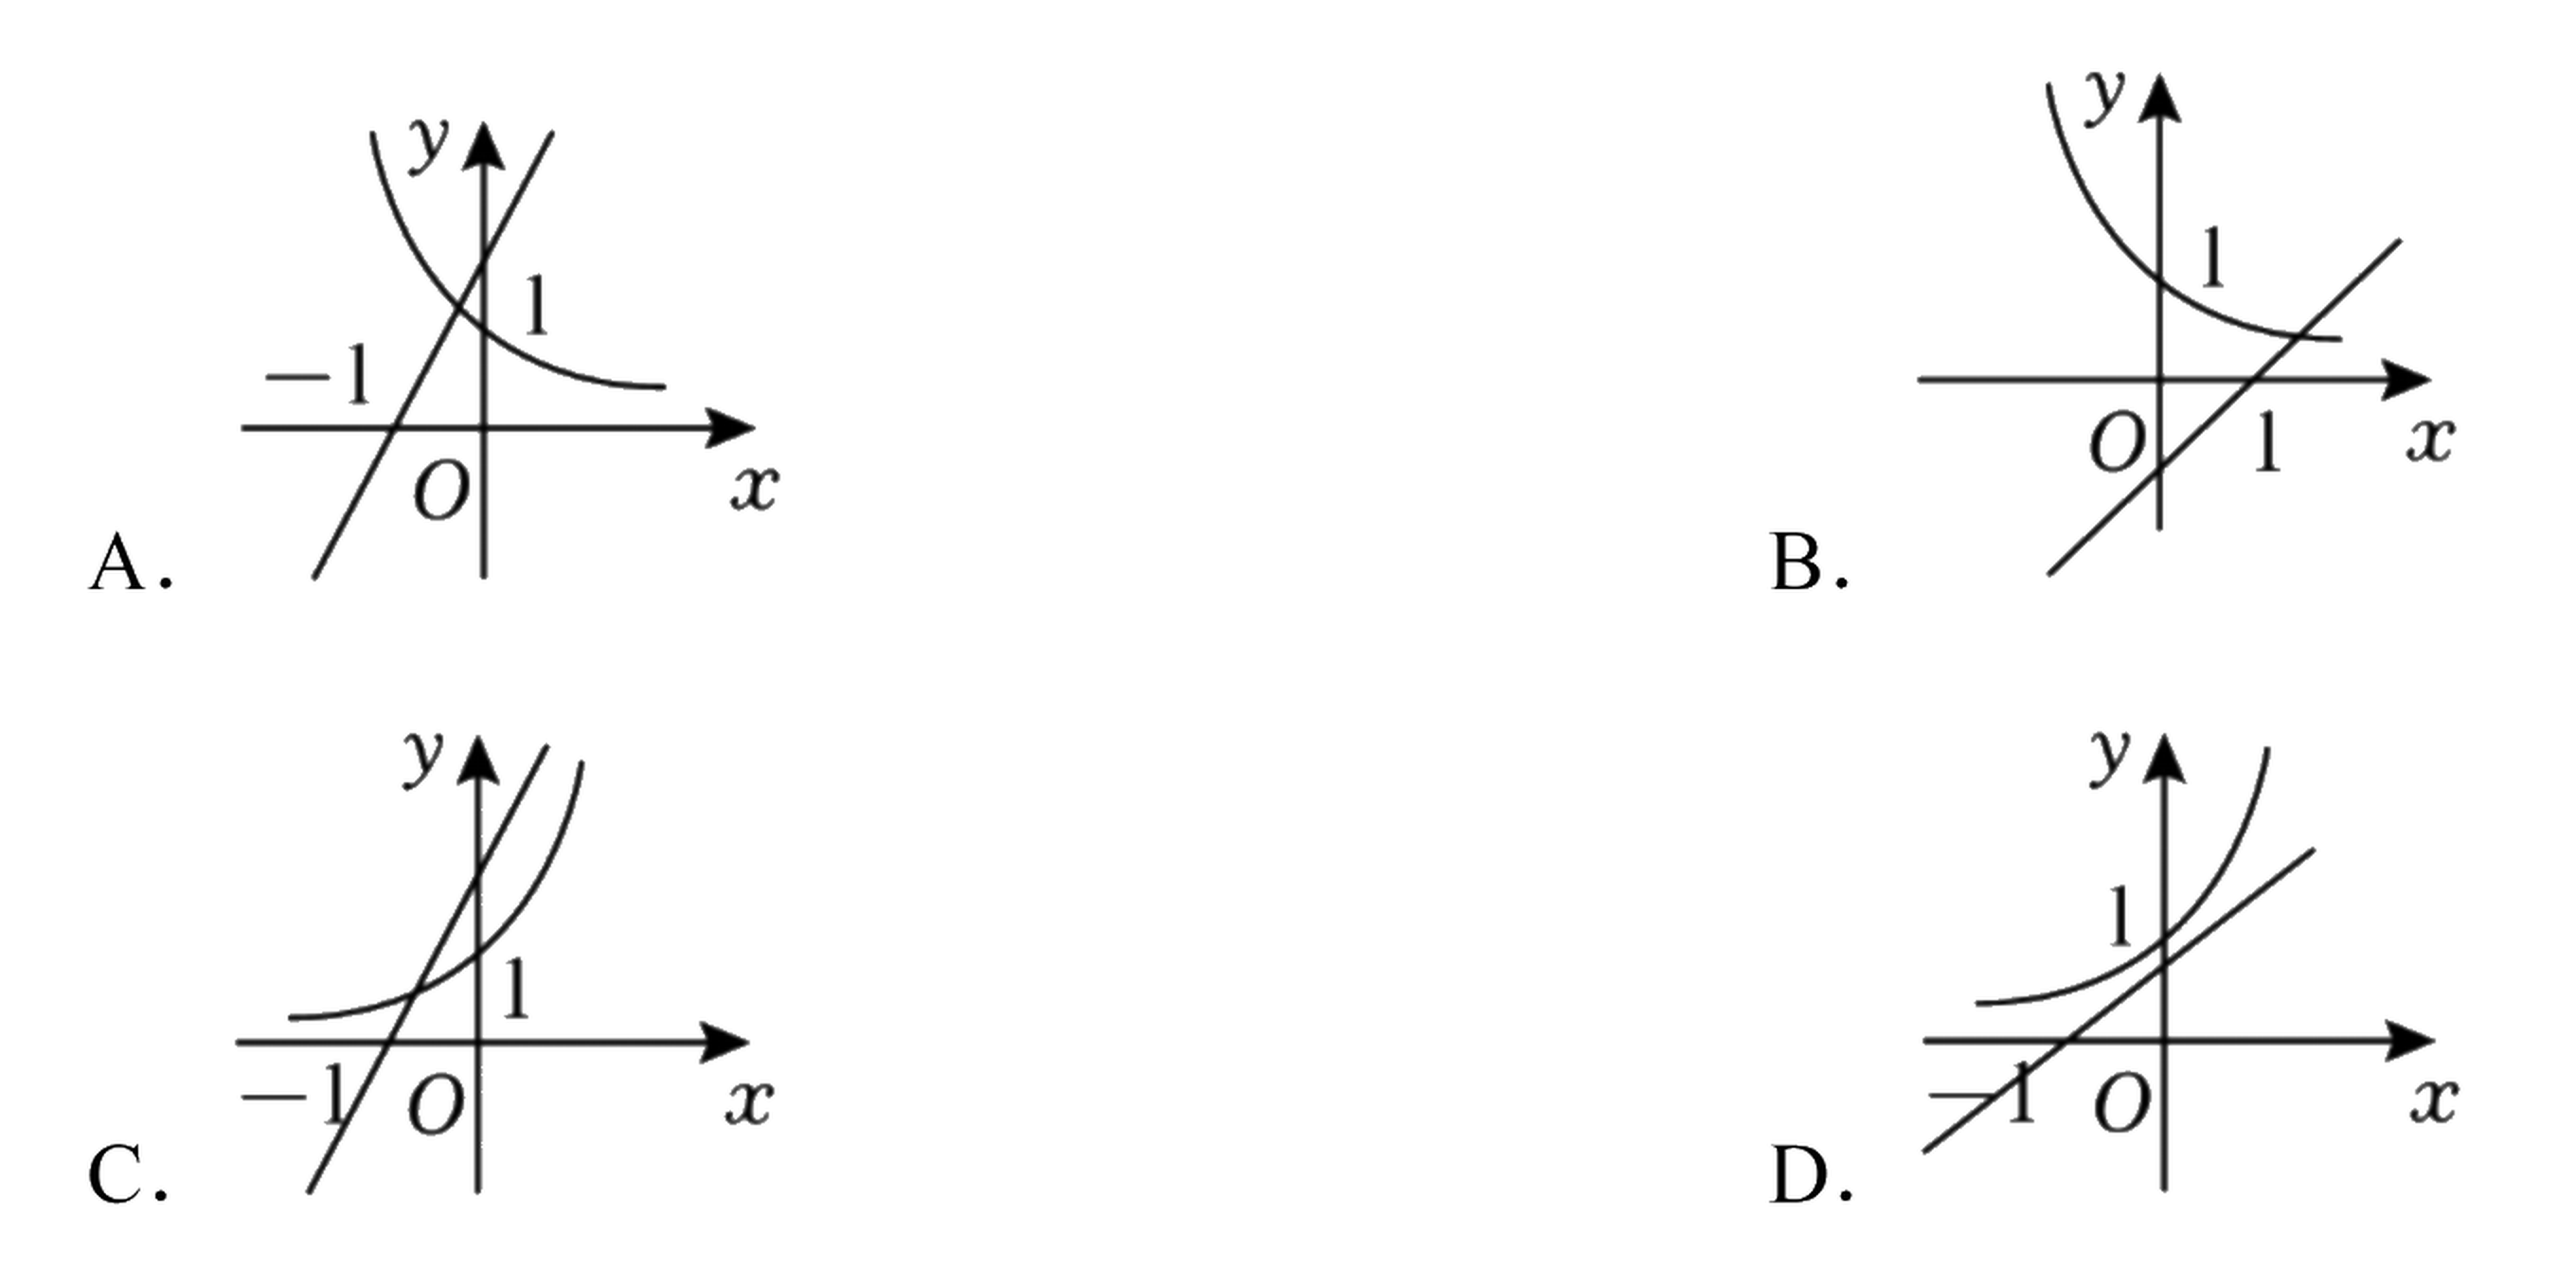
\includegraphics[width=0.80\textwidth]{figures/gao130_q15.png}
\end{center}

\ifanswer
\solbegin
\step{A 中，由指数函数 $y=a^x(a>0$ 且 $a\neq1)$ 图像递减得 $0<a<1$，}
\step{而一次函数 $y=a(x+1)$ 的图像与 $y$ 轴交点纵坐标为 $a>1$，二者矛盾，}
\step{所以 A 错；}
\step{由一次函数 $y=a(x+1)$ 的图像与 $x$ 轴交点横坐标为 $-1$，排除 B；}
\step{C 中，由指数函数 $y=a^x(a>0$ 且 $a\neq1)$ 图像递减得 $a>1$，}% 原卷"递减得 a>1"系笔误（应为"递增"），与 A 中"递减得 0<a<1"自相矛盾，照录
\step{而一次函数 $y=a(x+1)$ 的图像与 $y$ 轴交点纵坐标为 $a>1$，二者 $a$ 值吻合，}
\step{所以 C 对；}
\step{D 中，由一次函数 $y=a(x+1)$ 的图像得 $a=1$，与 $a>0$ 且 $a\neq1$ 矛盾，}
\step{所以 D 错.}
\step{故选 $C$.}
\solend
\fi

\item 设 $A_1$、$A_2$、$A_3$、$\cdots$、$A_7$ 是均含有 $2$ 个元素的集合，且 $A_1\cap A_7=\varnothing$，$A_i\cap A_{i+1}=\varnothing(i=1,2,3,\cdots,6)$，记 $B=A_1\cup A_2\cup A_3\cup\cdots\cup A_7$，则 $B$ 中元素个数的最小值是\mbox{（\quad）}

\keepwithprev
A. $4$\qquad B. $5$\qquad C. $6$\qquad D. $7$

\ifanswer
\solbegin
\step{取 $A_1=\{1,2\}$，$A_2=\{3,4\}$，$A_3=\{1,2\}$，$A_4=\{3,4\}$，$A_5=\{1,5\}$，$A_6=\{2,3\}$，$A_7=\{4,5\}$，}
\step{所以 $B$ 中元素个数的最小值是 $5$，故选 $B$.}
\solend
\fi

\end{enumerate}

\bigsec{三、解答题}

\begin{enumerate}
\setcounter{enumi}{16}

\item 已知全集为 $\R$，集合 $A=\{x\mid-2\leqslant x\leqslant5\}$，集合 $B=\{x\mid m-1\leqslant x\leqslant2m+1\}$．

(1) 求 $\overline{A}$；

(2) 若 $A\cup B=A$，求实数 $m$ 的取值范围．

\ifanswer
\solbegin
\step{(1) $(-\infty,-2)\cup(5,+\infty)$；}
\step{(2) 若 $A\cup B=A$，则 $B\subseteq A$，}
\step{当 $B=\varnothing$ 时，$m-1>2m+1$，解得 $m<-2$；}
\step{当 $B\neq\varnothing$ 时，$\begin{cases}m-1\leqslant2m+1\\m-1\geqslant-2\\2m+1\leqslant5\end{cases}$，解得 $-1\leqslant m\leqslant2$；}
\step{故实数 $m$ 的取值范围为 $\{m\mid-1\leqslant m\leqslant2$ 或 $m<-2\}$.}
\solend
\fi

\item 在不等式的应用中，有一些很基本而十分重要的不等式，如平均值不等式和三角不等式等，我们将其统称为基本不等式．

(1) 已知 $x$、$y$ 为正数，且 $2x+y=2$，求 $\dfrac1x+\dfrac2y$ 的最小值；

(2) 若关于 $x$ 的不等式 $\lvert x+1\rvert+\lvert2-x\rvert\geqslant a^2+a+1$ 对于一切实数 $x$ 都成立，求实数 $a$ 的取值范围．

\ifanswer
\solbegin
\step{(1) 因为 $x$、$y$ 为正数，且 $2x+y=2$，}
\step{所以 $\dfrac1x+\dfrac2y=\dfrac12\left(\dfrac1x+\dfrac2y\right)(2x+y)=\dfrac12\left(4+\dfrac yx+\dfrac{4x}y\right)\geqslant\dfrac12\left(4+2\sqrt{\dfrac yx\cdot\dfrac{4x}y}\right)=4$，}
\step{当且仅当 $\dfrac yx=\dfrac{4x}y$，即 $x=\dfrac12$，$y=1$ 时取等号，所以 $\dfrac1x+\dfrac2y$ 的最小值为 $4$；}
\step{(2) 由绝对值三角不等式得 $\lvert x+1\rvert+\lvert2-x\rvert\geqslant\lvert(x+1)+(2-x)\rvert=3$，}
\step{当且仅当 $-1\leqslant x\leqslant2$ 时取等号，所以 $\lvert x+1\rvert+\lvert2-x\rvert$ 的最小值为 $3$，}
\step{因为关于 $x$ 的不等式 $\lvert x+1\rvert+\lvert2-x\rvert\geqslant a^2+a+1$ 对于一切实数 $x$ 都成立，}
\step{所以 $a^2+a+1\leqslant3$，即 $a^2+a-2\leqslant0$，解得 $-2\leqslant a\leqslant1$，}
\step{所以实数 $a$ 的取值范围是 $[-2,1]$.}
\solend
\fi

\item 某医学专家为研究传染病传播中病毒细胞的发展规律，将病毒细胞注入一只小白鼠体内进行试验，经检测，病毒细胞的个数 $y$ 与天数 $x$ 的部分数据如表所示：

\begin{center}
\begin{tabular}{|c|c|c|c|c|c|c|c|}
\hline
天数 $(x)$ & $1$ & $2$ & $3$ & $4$ & $5$ & $6$ & $\cdots$ \\
\hline
病毒细胞的个数 $(y)$ & $1$ & $2$ & $4$ & $8$ & $16$ & $32$ & $\cdots$ \\
\hline
\end{tabular}
\end{center}

(1) 若病毒细胞的个数 $y$ 关于天数 $x$ 的变化规律可选用以下两个函数模型之一进行近似刻画：① $y=a\cdot b^x(a>0$，$b>0$，$b\neq1)$；② $y=a\cdot x^k(a\neq0)$．请结合表格中的数据，选择合适的函数模型，说明理由，并求出相应的函数表达式；

(2) 若该病毒细胞在小白鼠体内的个数超过 $10^8$，小白鼠将死亡，但注射某种药物，可杀死其体内 $98\%$ 的病毒细胞．则在 (1) 的条件下，为了使小白鼠在试验过程中不死亡，第一次最迟应在何时注射该种药物？（结果精确到天）

\ifanswer
\solbegin
\step{(1) 选择模型① $y=a\cdot b^x(a>0$，$b>0$，$b\neq1)$，理由如下：}
\step{观察表格数据，$y$ 的值随 $x$ 呈指数倍增：}
\step{$x=1$ 时，$y=1$，$x=2$ 时，$y=2$，$x=3$ 时，$y=4$，}
\step{后一天的病毒数是前一天的 $2$ 倍，符合指数增长的特征；}
\step{若选用幂函数模型 $y=a\cdot x^k$，代入前两组数据得 $a\cdot1^k=1$、$a\cdot2^k=2$，}
\step{解得 $a=1$，$k=1$，即 $y=x$，}
\step{但 $x=3$ 时，$y=3$ 与表格中 $y=4$ 严重不符，因此幂函数不匹配；}
\step{将 $(1,1)$ 代入 $y=a\cdot b^x$ 得 $a\cdot b=1$，}
\step{将 $(2,2)$ 代入得 $a\cdot b^2=2$，两式相除得 $b=2$，进而得 $a=\dfrac12$，}
\step{验证所有表格点均满足 $y=2^{x-1}$，最终函数表达式为 $y=2^{x-1}(x\in\N^*)$；}
\step{(2) 由题意得第一次注射药物前病毒细胞个数 $y$ 关于天数 $x(x\in\N^*)$ 的函数}
\step{关系式为 $y=2^{x-1}(x\in\N^*)$，}
\step{为了使小白鼠在试验过程中不死亡，则 $2^{x-1}\leqslant10^8$，}
\step{所以 $x-1\leqslant\log_210^8=8\log_210=\dfrac8{\lg2}$，解得 $x\leqslant1+\dfrac8{\lg2}\approx27.6$，}
\step{又 $x\in\N^*$，所以第一次最迟应在第 $27$ 天注射该种药物.}
\solend
\fi

\item 对在直角坐标系的第一象限内的任意两点 $(a,b)$，$(c,d)$ 作如下定义：$\dfrac ab>\dfrac cd$，那么称点 $(a,b)$ 是点 $(c,d)$ 的“上位点”，同时点 $(c,d)$ 是点 $(a,b)$ 的“下位点”．

(1) 试写出点 $(3,5)$ 的一个“上位点”坐标和一个“下位点”坐标；

(2) 设 $a$、$b$、$c$、$d$ 均为正数，且点 $(a,b)$ 是点 $(c,d)$ 的上位点，请判断点 $P(a+c,b+d)$ 是否既是点 $(a,b)$ 的“下位点”又是点 $(c,d)$ 的“上位点”，如果是，请证明；如果不是，请说明理由；

(3) 设正整数 $n$ 满足以下条件：对任意实数 $m\in\{t\mid0<t<4,t\in\Z\}$，总存在正整数 $k$，使得点 $(n,k)$ 既是点 $(4,m)$ 的“下位点”，又是点 $(5,m+1)$ 的“上位点”，求正整数 $n$ 的最小值．

\ifanswer
\solbegin
\step{(1) 由 $\dfrac34>\dfrac35>\dfrac36$ 得点 $(3,5)$ 的一个“上位点”的坐标为 $(3,4)$，}
\step{一个“下位点”的坐标为 $(3,6)$.}
\step{(2) 是，证明如下：}
\step{因为 $a$、$b$、$c$、$d$ 均为正数，点 $(a,b)$ 是点 $(c,d)$ 的“上位点”，}
\step{所以 $\dfrac ab>\dfrac cd$，所以 $ad>bc$，}
\step{因为 $\dfrac{a+c}{b+d}-\dfrac ab=\dfrac{b(a+c)-a(b+d)}{b(b+d)}=\dfrac{bc-ad}{b(b+d)}<0$，所以 $\dfrac{a+c}{b+d}<\dfrac ab$，}
\step{点 $P(a+c,b+d)$ 是点 $(a,b)$ 的“下位点”，}
\step{因为 $\dfrac{a+c}{b+d}-\dfrac cd=\dfrac{d(a+c)-c(b+d)}{d(b+d)}=\dfrac{ad-bc}{d(b+d)}>0$.}
\step{所以 $\dfrac{a+c}{b+d}>\dfrac cd$ 点 $P(a+c,b+d)$ 是点 $(c,d)$ 的“上位点”；}
\step{所以 $P(a+c,b+d)$ 既是点 $(a,b)$ 的“下位点”又是点 $(c,d)$ 的“上位点”；}
\step{(3) 由题意得 $m=1,2,3$，}
\step{由题意存在正整数 $k$：$\dfrac5{m+1}<\dfrac nk<\dfrac4m$，所以 $\begin{cases}\dfrac n4<k<\dfrac{2n}5(m=1)\\\dfrac n2<k<\dfrac{3n}5(m=2)\\\dfrac{3n}4<k<\dfrac{4n}5(m=3)\end{cases}$，}
\step{检验：$n=1,2,\cdots,8$ 不能同时找到整数 $k$，}
\step{$n=9$：$m=1$ 取 $k=3$，$m=2$ 取 $k=5$，$m=3$ 取 $k=7$，均满足，}
\step{所以正整数 $n$ 的最小值为 $9$.}
\solend
\fi

\end{enumerate}

\end{document}
"
%
% ① 原始材料：微信公众号"魔都数学加油站"文章，连载"27学年高一140"，原文标题
% "27学年高一140——2026-2027年上海市北郊高级中学高一上期中"；
% 原文链接：https://mp.weixin.qq.com/s/XBEYuTheiBoqu15dtLuD6A。
%   ★ 编号不一致说明：公众号连载号印"140"，与上一批已入库的"高一140 甘泉外国语"
%   （同一公众号另一篇文章、同为期中卷）撞号，系公众号笔误/重复。本仓库数字编号
%   02—143 中"高一130"一直空缺（连载 130 暂未见原文），故将本卷本地编号定为"高一130"、
%   填补该空缺，使数字编号连续（basename 全程为 高一130_北郊高级中学_期中）；
%   连载号 143 归正牌卷"上海中学 高一上期中"；本卷连载号仍印 140，见材料流转表。
%   卷面标题印"2026-2027 年北郊高级中学高一上期中"（卷面只有学校名、不含"上海市"、
%   不含任何期号/连载号），本稿照卷面录入；粉红色水印"魔都数学加油站"及页脚未录入。
% 正文为 9 张 PNG 页（01、04、05、06、09 为 2560x3620；02、03、07、08 为 4762x6735，
% 同一篇各页分辨率不同，逐页按各自分辨率放大核对），题目下印有【解析】，为讲评版。
% 题目、解析均据原图转录。
%
% 卷首标题：原卷印作"2026-2027 年北郊高级中学高一上期中"，年份区间按全稿惯例排
% en dash；原卷未印副标题，本卷为期中卷、跨集合与常用逻辑用语／不等式／函数三章，
% 按题目内容补出"集合与常用逻辑用语、不等式、函数"（与 125／126／128／129／131／132／133
% 同期中卷口径相同）。
%
% 题号体例：本卷共 18 题——一、填空题 3—12（10 题）、二、选择题 13—16（4 题）、
% 三、解答题 17—20（4 题）。三节分别 \setcounter{enumi}{2}／{12}／{16}。
% 原卷从第 3 题起、无第 1、2 题、**无第 21 题**（第 20 题解析续至 09 页，末行
% "所以正整数 n 的最小值为 9."，09 页下半页整片空白＋水印收尾、无第 10 页），本稿保留原题号。
%
% ② 与原卷的排版差异：
%   ① 原文从第 3 题起，本稿保留原题号；原卷止于第 20 题、无第 21 题、无附加题节；
%   ② 原卷每题下直接印【解析】，本稿按全稿惯例置于答案版；全卷 18 题均印【解析】、
%      无独立【答案】段，四道选择题答案在解析末句"故选 C／D／C／B"，括号
%      \mbox{（\quad）} 留空、不另提 \ans{}；全卷 0 处 \ans{}，答案版【解析】标记数 18＝题数；
%   ③ 原卷未印副标题，本稿按"知识模块"口径补出；
%   ④ 原卷填空横线按全稿惯例排为 \blankline[4.4em]；选择题括号排 \mbox{（\quad）}、
%      每个选项段前按惯例加 \keepwithprev；解答题不留作答区、不加 \anspace（讲评版）；
%   ⑤ 原卷数集排斜体 $R$／$N$，按全稿惯例改 \R／\N；空集记号 \varnothing；
%      绝对值排 \lvert…\rvert，集合描述竖线排 \mid；不等号按全稿惯例排 \leqslant／\geqslant；
%      补集照原卷上划线 \overline{A}；
%   ⑥ 1 幅插图 + 1 张印刷表格：第 15 题四幅坐标函数图象选项（04 页）取原卷截图
%      去粉色水印、去色、按原卷 2x2 排布合并为 figures/gao130_q15.png（非插图重绘），
%      放在 \keepwithprev 之后 \begin{center} 内、三版都出；第 19 题 (1) 印刷数据表格
%      （07 页，天数 x 1—6／病毒细胞个数 y 1/2/4/8/16/32）按原卷用 tabular 重排、
%      题干内三版都出（非插图）。
%      第 15 题是"二、选择题"节内带大图块的第三题（Q13 为节首题但无图），
%      在 \bigsec{二、选择题} 之前加 \needvspace{11cm} 连节标题一起量、Q15 \item 之前
%      加 \needvspace{9cm}——守卫必须放在 \bigsec 之前，放标题之后会让"二、选择题"
%      孤立在页末（B 类，照 高一26／40／59／136／140 成例）；三版切页审计均"合计异常：无"；
%   ⑦ 子题标号 (1)(2)(3) 原卷用半角括号，照录；圈数字 ①②③④ 照录；
%      数学式内半角逗号照录（如第 14 题 $(a>0,a\neq1)$、第 16 题
%      $(i=1,2,3,\cdots,6)$、第 20 题 $m=1,2,3$ 等）；
%      行末西文句点按全稿惯例照录；
%   ⑧ 题干中的中文弯引号按原卷照录（Q12"变项和"、Q20"上位点""下位点"等），
%      注释内一律 ASCII 引号；原卷"图像"用词逐处照录（Q9、Q15 均作"图像"）。
%
% ③ 行数复核：一条 \step = 原卷解析的一个印刷行（cases 块与 tabular 各作一个印刷行计）。
%   逐题 \step 条数，合计 98 条（Q3:3 Q4:2 Q5:2 Q6:1 Q7:1 Q8:3 Q9:5 Q10:10 Q11:6
%   Q12:7 Q13:1 Q14:2 Q15:10 Q16:2 Q17:5 Q18:8 Q19:15 Q20:15），与原卷印刷行逐题相等。
%
% ④ 判别式／子集符号结论：
%   判别式：全卷未出现判别式记号（无 $\Delta$、无 $\triangle$）；
%   子集符号：第 4 题题干"$B\subseteq A$"、第 4 题【解析】"$B\subseteq A$"、
%      第 17 题 (2)【解析】"$B\subseteq A$"三处原卷均印带下划线 $\subseteq$，逐处
%      放大核对、照录 \subseteq；全卷未出现单线 \subset。
%
% ⑤ 原卷存疑照录（均照录未改，正文对应处另有 % 注）：
%   ① 第 15 题【解析】"C 中，由指数函数 $y=a^x$ 图像递减得 $a>1$"——"递减"应为
%      "递增"之误（与同题 A 中"递减得 $0<a<1$"自相矛盾），原卷如此，照录并加注；
%   ② 第 16 题题干"$A_1\cap A_7=\varnothing$""$A_i\cap A_{i+1}=\varnothing$"
%      的空集记号与解析所列各集合逐处照录；
%   ③ 第 19 题 (2) 题干"可杀死其体内 98% 的病毒细胞"、解析 (2) 只按 $y=2^{x-1}$
%      与 $10^8$ 比较（未另计 98%），照录不补步。
%
% ⑥ 跨页续印按题合并：Q8 题干在 01 页末、解析在 02 页；Q9 题干在 02 页、
%   解析在 02 页；Q10 题干在 02 页、解析前 5 行在 02—03 页、后 5 行在 03 页；
%   Q12 题干跨 03 页、解析首 5 行在 03 页末、末行在 04 页；Q15 题干在 04 页、
%   四幅图与解析前段在 04 页、解析续在 05 页；Q17 解析跨 05—06 页；Q18 题干与
%   (1) 解析在 06 页、(2) 解析在 06—07 页；Q19 表格在 07 页、解析跨 07—08 页；
%   Q20 定义与三小问在 08 页、解析 (1)(2) 在 08—09 页、解析 (3) 在 09 页；
%   本稿按题连排，不丢行。
%
\documentclass[a4paper,11pt]{article}
\usepackage{common}

\begin{document}

\examtitlest[3]{2026--2027 年北郊高级中学高一上期中}{集合与常用逻辑用语、不等式、函数}

\bigsec{一、填空题}

\begin{enumerate}
\setcounter{enumi}{2}

\item 不等式 $\dfrac{x-3}{x+1}<2$ 的解集为\blankline[4.4em].

\ifanswer
\solbegin
\step{不等式 $\dfrac{x-3}{x+1}<2$ 可化为 $\dfrac{x-3}{x+1}-2<0$，即 $\dfrac{x-3-2(x+1)}{x+1}<0$，}
\step{化简为 $\dfrac{x+5}{x+1}>0$，解得 $x<-5$ 或 $x>-1$，}
\step{所以不等式的解集为 $\{x\mid x<-5$ 或 $x>-1\}$.}
\solend
\fi

\item 已知集合 $A=\{x\mid0<x<a\}$，$B=\{x\mid1<x<2\}$，若 $B\subseteq A$，则实数 $a$ 的取值范围为\blankline[4.4em].

\ifanswer
\solbegin
\step{已知集合 $A=\{x\mid0<x<a\}$，$B=\{x\mid1<x<2\}$，}
\step{若 $B\subseteq A$，则 $a\geqslant2$，所以实数 $a$ 的取值范围是 $\{a\mid a\geqslant2\}$.}
\solend
\fi

\item 已知关于 $x$ 的方程 $x^2+x+c=0$ 的两个实数根为 $x_1$、$x_2$，若 $x_1^2x_2+x_2^2x_1=3$，则实数 $c=$\blankline[4.4em].

\ifanswer
\solbegin
\step{由韦达定理得 $x_1+x_2=-1$，$x_1x_2=c$，所以 $x_1^2x_2+x_2^2x_1=(x_1+x_2)x_1x_2=-c=3$，}
\step{所以 $c=-3$.}
\solend
\fi

\item 已知 $10^x=3$，$10^y=64$，则 $10^{x-\frac y3}=$\blankline[4.4em].

\ifanswer
\solbegin
\step{$10^{x-\frac y3}=10^x\div\sqrt[3]{10^y}=\dfrac34$.}
\solend
\fi

\item 若 $\lg2=a$，则可用 $a$ 表示 $\log_280=$\blankline[4.4em].

\ifanswer
\solbegin
\step{$\log_280=\dfrac{\lg80}{\lg2}=\dfrac{\lg10+\lg8}{\lg2}=\dfrac{1+3\lg2}{\lg2}=\dfrac{1+3a}{a}$.}
\solend
\fi

\item 已知 $a+2b=1$，则 $3^a+9^b$ 的最小值为\blankline[4.4em].

\ifanswer
\solbegin
\step{因为 $a+2b=1$，所以 $3^a+9^b=3^a+3^{2b}\geqslant2\sqrt{3^a\cdot3^{2b}}=2\sqrt{3^{a+2b}}=2\sqrt3$，}
\step{当且仅当 $3^a=3^{2b}$，且 $a+2b=1$，即 $a=\dfrac12$，$b=\dfrac14$ 时取等号，}
\step{故最小值为 $2\sqrt3$.}
\solend
\fi

\item 下列函数的图像关于原点成中心对称，且在区间 $(0,+\infty)$ 上是严格增函数的是\blankline[4.4em]（请填写全部正确的序号）.

① $y=\sqrt{x}$；② $y=\sqrt[3]{x}$；③ $y=x^{\frac23}$；④ $y=x^{-\frac13}$.

\ifanswer
\solbegin
\step{① $y=\sqrt{x}$ 的定义域为 $[0,+\infty)$，故其图像不关于原点成中心对称，①错误；}
\step{② $y=\sqrt[3]{x}$ 是奇函数，且在区间 $(0,+\infty)$ 上是严格增函数，②正确；}
\step{③ $y=x^{\frac23}$ 是偶函数，其图像关于 $y$ 轴对称，不关于原点成中心对称，③错误；}
\step{④由于幂指数 $-\dfrac13<0$，故 $y=x^{-\frac13}$ 在区间 $(0,+\infty)$ 上是严格减函数，④错误.}
\step{故正确的是②.}
\solend
\fi

\item 设 $a>0$ 且 $a\neq1$，若函数 $y=a^{2x}+2a^x-3$ 在区间 $[-1,1]$ 上的最大值为 $21$，则实数 $a$ 的值为\blankline[4.4em].

\ifanswer
\solbegin
\step{令 $t=a^x$，$x\in[-1,1]$，}
\step{当 $a>1$ 时，$t=a^x$ 严格增，则 $t\in\left[\dfrac1a,a\right]$，}
\step{则函数 $y=t^2+2t-3$，对称轴为 $t=-1$，}
\step{所以函数 $y=t^2+2t-3$ 在 $\left[\dfrac1a,a\right]$ 上严格增，}
\step{所以当 $t=a$ 时，$y$ 取得最大值 $a^2+2a-3=21$，解得 $a=4$ 或 $-6$（舍去）；}
\step{当 $0<a<1$ 时，$t=a^x$ 严格减，则 $t\in\left[a,\dfrac1a\right]$，}
\step{则函数 $y=t^2+2t-3$，对称轴为 $t=-1$，}
\step{所以函数 $y=t^2+2t-3$ 在 $\left[a,\dfrac1a\right]$ 上严格增，}
\step{所以当 $t=\dfrac1a$ 时，$y$ 取得最大值 $\dfrac1{a^2}+\dfrac2a-3=21$，解得 $a=\dfrac14$ 或 $-\dfrac16$（舍去）；}
\step{综上所述，实数 $a$ 的值为 $4$ 或 $\dfrac14$.}
\solend
\fi

\item 在关于 $x$ 的不等式 $x^2+(m+1)x+m<0$ 的解集中恰有两个整数，则实数 $m$ 的取值范围是\blankline[4.4em].

\ifanswer
\solbegin
\step{关于 $x$ 的不等式 $x^2+(m+1)x+m<0$ 可化为 $(x+1)(x+m)<0$，}
\step{当 $m>1$ 时，$-m<-1$，解不等式得 $-m<x<-1$；}
\step{当 $m<1$ 时，$-m>-1$，解不等式得 $-1<x<-m$；}
\step{由不等式的解集中恰有两个整数，}
\step{则 $-4\leqslant-m<-3$ 或 $1<-m\leqslant2$，即 $3<m\leqslant4$ 或 $-2\leqslant m<-1$，}
\step{所以 $m$ 的取值范围是 $[-2,-1)\cup(3,4]$.}
\solend
\fi

\item 已知集合 $M$ 的元素均为正整数，定义集合 $M$ 的“变项和”为：将 $M$ 中每个元素 $m$ 都乘以 $(-1)^m$ 后再求和．若集合 $A=\{n\mid1\leqslant n\leqslant20,n\in\N\}$，则集合 $A$ 的所有非空子集的“变项和”的总和为\blankline[4.4em].

\ifanswer
\solbegin
\step{集合 $A=\{n\mid1\leqslant n\leqslant20,n\in\N\}$ 中一共有 $20$ 个元素，}
\step{固定选中 $k$，剩下 $19$ 个元素任选，共 $2^{19}$ 个子集包含 $k$，每个 $k$ 贡献 $(-1)^k\cdot k\cdot2^{19}$，}
\step{$A=\{1,2,\cdots,20\}$，}
\step{奇数 $k=1,3,\cdots,19$，共 $10$ 个，$(-1)^k\cdot k=-k$，}
\step{偶数 $k=2,4,\cdots,20$，共 $10$ 个，$(-1)^k\cdot k=k$，}
\step{所以集合 $A$ 的所有非空子集的“变项和”的总和}
\step{为 $S=2^{19}\times[(-1+2)+(-3+4)+\cdots+(-19+20)]=2^{19}\times10=524880$.}
\solend
\fi

\end{enumerate}

% 第 15 题四幅图是"二、选择题"节内大图块；守卫须放在 \bigsec 之前连节标题一起量，
% 否则"二、选择题"会孤立在页末（B 类，照 高一26／40／59／136／140 成例）
\needvspace{11cm}
\bigsec{二、选择题}

\begin{enumerate}
\setcounter{enumi}{12}

\item 设 $ab>0$，则“$a>b$”是“$\dfrac1a<\dfrac1b$”的\mbox{（\quad）}

\keepwithprev
A. 充分非必要条件\qquad B. 必要非充分条件

C. 充要条件\qquad D. 既非充分也非必要条件

\ifanswer
\solbegin
\step{因为 $ab>0$，所以 $a>b\Leftrightarrow\dfrac1a<\dfrac1b$，故选 $C$.}
\solend
\fi

\item 已知 $A=\log_ax$，$B=\log_ay(a>0,a\neq1)$，则 $\log_a\dfrac{x^2}{\sqrt y}=$\mbox{（\quad）}

\keepwithprev
A. $\dfrac{A^2}{\sqrt B}$\qquad B. $2A^2B$\qquad C. $4AB$\qquad D. $2A-\dfrac12B$

\ifanswer
\solbegin
\step{由已知得 $x=a^A$，$y=a^B$，}
\step{所以 $\log_a\dfrac{x^2}{\sqrt y}=\log_a\dfrac{(a^A)^2}{\sqrt{a^B}}=\log_a\dfrac{a^{2A}}{a^{\frac12B}}=\log_a a^{2A-\frac12B}=2A-\dfrac12B$. 故选 $D$.}
\solend
\fi

% 第 15 题四幅坐标函数图象选项是一整块，守卫放在 \item 之前
\needvspace{9cm}
\item 在同一平面直角坐标系中，指数函数 $y=a^x(a>0$ 且 $a\neq1)$ 和一次函数 $y=a(x+1)$ 的图像关系可能是\mbox{（\quad）}

\keepwithprev
\begin{center}
% 四幅坐标函数图象选项取原卷 04 页截图去粉色水印、去色，按原卷 2x2 排布合并为一张
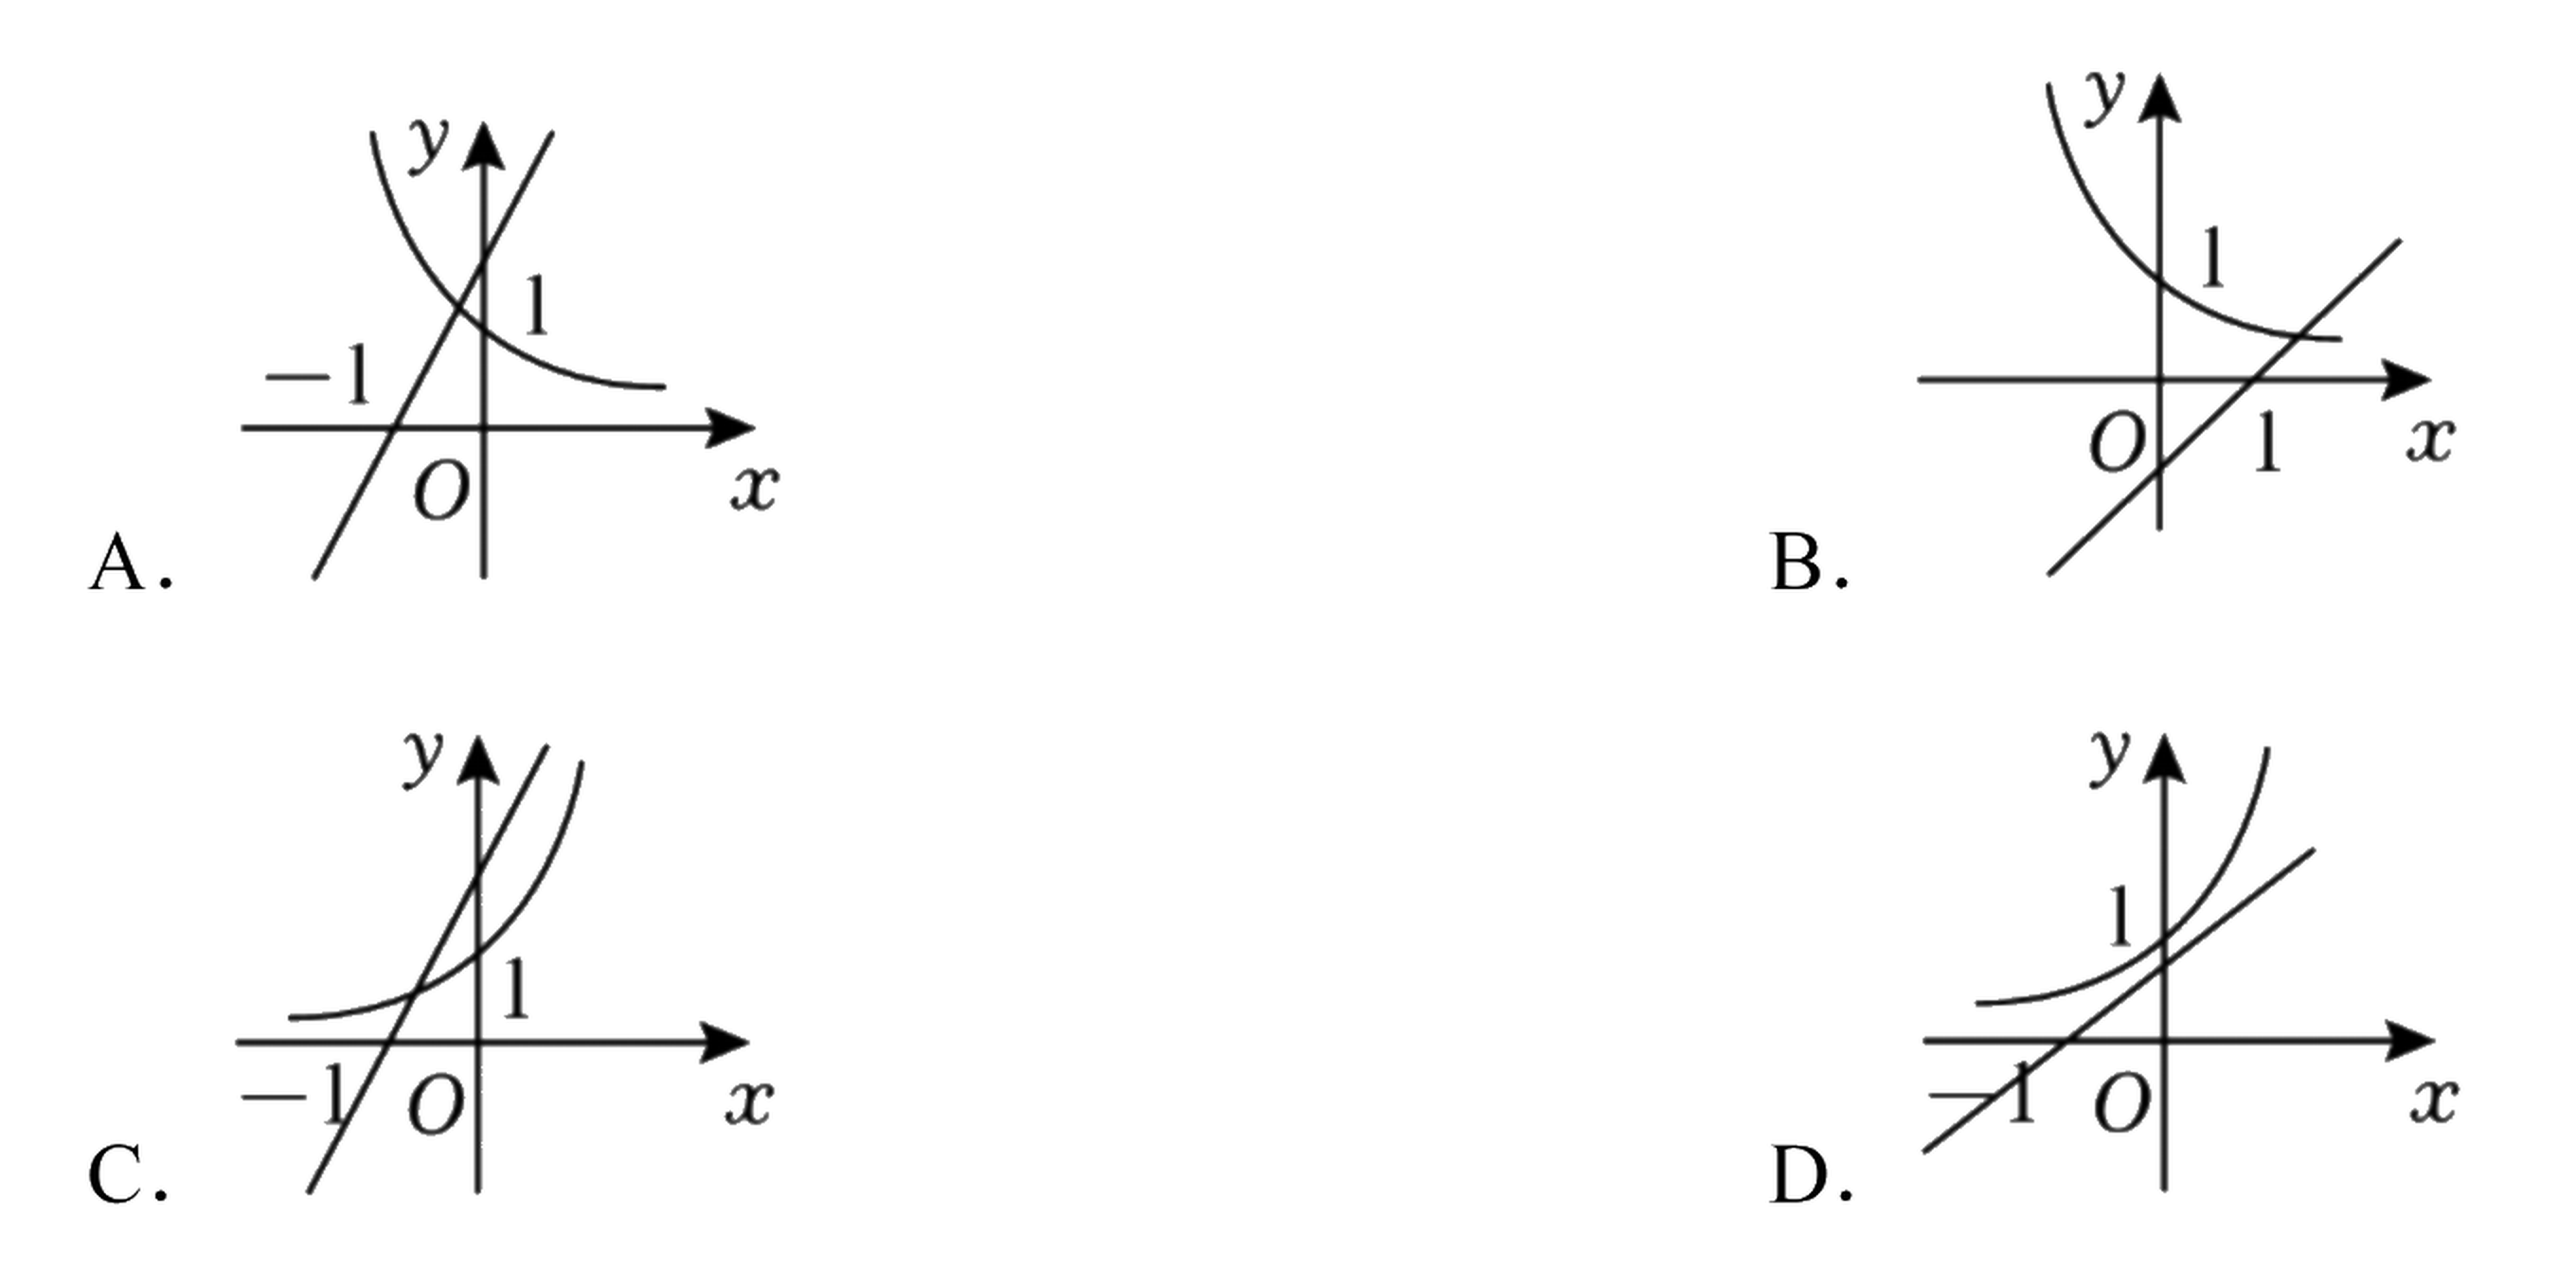
\includegraphics[width=0.80\textwidth]{figures/gao130_q15.png}
\end{center}

\ifanswer
\solbegin
\step{A 中，由指数函数 $y=a^x(a>0$ 且 $a\neq1)$ 图像递减得 $0<a<1$，}
\step{而一次函数 $y=a(x+1)$ 的图像与 $y$ 轴交点纵坐标为 $a>1$，二者矛盾，}
\step{所以 A 错；}
\step{由一次函数 $y=a(x+1)$ 的图像与 $x$ 轴交点横坐标为 $-1$，排除 B；}
\step{C 中，由指数函数 $y=a^x(a>0$ 且 $a\neq1)$ 图像递减得 $a>1$，}% 原卷"递减得 a>1"系笔误（应为"递增"），与 A 中"递减得 0<a<1"自相矛盾，照录
\step{而一次函数 $y=a(x+1)$ 的图像与 $y$ 轴交点纵坐标为 $a>1$，二者 $a$ 值吻合，}
\step{所以 C 对；}
\step{D 中，由一次函数 $y=a(x+1)$ 的图像得 $a=1$，与 $a>0$ 且 $a\neq1$ 矛盾，}
\step{所以 D 错.}
\step{故选 $C$.}
\solend
\fi

\item 设 $A_1$、$A_2$、$A_3$、$\cdots$、$A_7$ 是均含有 $2$ 个元素的集合，且 $A_1\cap A_7=\varnothing$，$A_i\cap A_{i+1}=\varnothing(i=1,2,3,\cdots,6)$，记 $B=A_1\cup A_2\cup A_3\cup\cdots\cup A_7$，则 $B$ 中元素个数的最小值是\mbox{（\quad）}

\keepwithprev
A. $4$\qquad B. $5$\qquad C. $6$\qquad D. $7$

\ifanswer
\solbegin
\step{取 $A_1=\{1,2\}$，$A_2=\{3,4\}$，$A_3=\{1,2\}$，$A_4=\{3,4\}$，$A_5=\{1,5\}$，$A_6=\{2,3\}$，$A_7=\{4,5\}$，}
\step{所以 $B$ 中元素个数的最小值是 $5$，故选 $B$.}
\solend
\fi

\end{enumerate}

\bigsec{三、解答题}

\begin{enumerate}
\setcounter{enumi}{16}

\item 已知全集为 $\R$，集合 $A=\{x\mid-2\leqslant x\leqslant5\}$，集合 $B=\{x\mid m-1\leqslant x\leqslant2m+1\}$．

(1) 求 $\overline{A}$；

(2) 若 $A\cup B=A$，求实数 $m$ 的取值范围．

\ifanswer
\solbegin
\step{(1) $(-\infty,-2)\cup(5,+\infty)$；}
\step{(2) 若 $A\cup B=A$，则 $B\subseteq A$，}
\step{当 $B=\varnothing$ 时，$m-1>2m+1$，解得 $m<-2$；}
\step{当 $B\neq\varnothing$ 时，$\begin{cases}m-1\leqslant2m+1\\m-1\geqslant-2\\2m+1\leqslant5\end{cases}$，解得 $-1\leqslant m\leqslant2$；}
\step{故实数 $m$ 的取值范围为 $\{m\mid-1\leqslant m\leqslant2$ 或 $m<-2\}$.}
\solend
\fi

\item 在不等式的应用中，有一些很基本而十分重要的不等式，如平均值不等式和三角不等式等，我们将其统称为基本不等式．

(1) 已知 $x$、$y$ 为正数，且 $2x+y=2$，求 $\dfrac1x+\dfrac2y$ 的最小值；

(2) 若关于 $x$ 的不等式 $\lvert x+1\rvert+\lvert2-x\rvert\geqslant a^2+a+1$ 对于一切实数 $x$ 都成立，求实数 $a$ 的取值范围．

\ifanswer
\solbegin
\step{(1) 因为 $x$、$y$ 为正数，且 $2x+y=2$，}
\step{所以 $\dfrac1x+\dfrac2y=\dfrac12\left(\dfrac1x+\dfrac2y\right)(2x+y)=\dfrac12\left(4+\dfrac yx+\dfrac{4x}y\right)\geqslant\dfrac12\left(4+2\sqrt{\dfrac yx\cdot\dfrac{4x}y}\right)=4$，}
\step{当且仅当 $\dfrac yx=\dfrac{4x}y$，即 $x=\dfrac12$，$y=1$ 时取等号，所以 $\dfrac1x+\dfrac2y$ 的最小值为 $4$；}
\step{(2) 由绝对值三角不等式得 $\lvert x+1\rvert+\lvert2-x\rvert\geqslant\lvert(x+1)+(2-x)\rvert=3$，}
\step{当且仅当 $-1\leqslant x\leqslant2$ 时取等号，所以 $\lvert x+1\rvert+\lvert2-x\rvert$ 的最小值为 $3$，}
\step{因为关于 $x$ 的不等式 $\lvert x+1\rvert+\lvert2-x\rvert\geqslant a^2+a+1$ 对于一切实数 $x$ 都成立，}
\step{所以 $a^2+a+1\leqslant3$，即 $a^2+a-2\leqslant0$，解得 $-2\leqslant a\leqslant1$，}
\step{所以实数 $a$ 的取值范围是 $[-2,1]$.}
\solend
\fi

\item 某医学专家为研究传染病传播中病毒细胞的发展规律，将病毒细胞注入一只小白鼠体内进行试验，经检测，病毒细胞的个数 $y$ 与天数 $x$ 的部分数据如表所示：

\begin{center}
\begin{tabular}{|c|c|c|c|c|c|c|c|}
\hline
天数 $(x)$ & $1$ & $2$ & $3$ & $4$ & $5$ & $6$ & $\cdots$ \\
\hline
病毒细胞的个数 $(y)$ & $1$ & $2$ & $4$ & $8$ & $16$ & $32$ & $\cdots$ \\
\hline
\end{tabular}
\end{center}

(1) 若病毒细胞的个数 $y$ 关于天数 $x$ 的变化规律可选用以下两个函数模型之一进行近似刻画：① $y=a\cdot b^x(a>0$，$b>0$，$b\neq1)$；② $y=a\cdot x^k(a\neq0)$．请结合表格中的数据，选择合适的函数模型，说明理由，并求出相应的函数表达式；

(2) 若该病毒细胞在小白鼠体内的个数超过 $10^8$，小白鼠将死亡，但注射某种药物，可杀死其体内 $98\%$ 的病毒细胞．则在 (1) 的条件下，为了使小白鼠在试验过程中不死亡，第一次最迟应在何时注射该种药物？（结果精确到天）

\ifanswer
\solbegin
\step{(1) 选择模型① $y=a\cdot b^x(a>0$，$b>0$，$b\neq1)$，理由如下：}
\step{观察表格数据，$y$ 的值随 $x$ 呈指数倍增：}
\step{$x=1$ 时，$y=1$，$x=2$ 时，$y=2$，$x=3$ 时，$y=4$，}
\step{后一天的病毒数是前一天的 $2$ 倍，符合指数增长的特征；}
\step{若选用幂函数模型 $y=a\cdot x^k$，代入前两组数据得 $a\cdot1^k=1$、$a\cdot2^k=2$，}
\step{解得 $a=1$，$k=1$，即 $y=x$，}
\step{但 $x=3$ 时，$y=3$ 与表格中 $y=4$ 严重不符，因此幂函数不匹配；}
\step{将 $(1,1)$ 代入 $y=a\cdot b^x$ 得 $a\cdot b=1$，}
\step{将 $(2,2)$ 代入得 $a\cdot b^2=2$，两式相除得 $b=2$，进而得 $a=\dfrac12$，}
\step{验证所有表格点均满足 $y=2^{x-1}$，最终函数表达式为 $y=2^{x-1}(x\in\N^*)$；}
\step{(2) 由题意得第一次注射药物前病毒细胞个数 $y$ 关于天数 $x(x\in\N^*)$ 的函数}
\step{关系式为 $y=2^{x-1}(x\in\N^*)$，}
\step{为了使小白鼠在试验过程中不死亡，则 $2^{x-1}\leqslant10^8$，}
\step{所以 $x-1\leqslant\log_210^8=8\log_210=\dfrac8{\lg2}$，解得 $x\leqslant1+\dfrac8{\lg2}\approx27.6$，}
\step{又 $x\in\N^*$，所以第一次最迟应在第 $27$ 天注射该种药物.}
\solend
\fi

\item 对在直角坐标系的第一象限内的任意两点 $(a,b)$，$(c,d)$ 作如下定义：$\dfrac ab>\dfrac cd$，那么称点 $(a,b)$ 是点 $(c,d)$ 的“上位点”，同时点 $(c,d)$ 是点 $(a,b)$ 的“下位点”．

(1) 试写出点 $(3,5)$ 的一个“上位点”坐标和一个“下位点”坐标；

(2) 设 $a$、$b$、$c$、$d$ 均为正数，且点 $(a,b)$ 是点 $(c,d)$ 的上位点，请判断点 $P(a+c,b+d)$ 是否既是点 $(a,b)$ 的“下位点”又是点 $(c,d)$ 的“上位点”，如果是，请证明；如果不是，请说明理由；

(3) 设正整数 $n$ 满足以下条件：对任意实数 $m\in\{t\mid0<t<4,t\in\Z\}$，总存在正整数 $k$，使得点 $(n,k)$ 既是点 $(4,m)$ 的“下位点”，又是点 $(5,m+1)$ 的“上位点”，求正整数 $n$ 的最小值．

\ifanswer
\solbegin
\step{(1) 由 $\dfrac34>\dfrac35>\dfrac36$ 得点 $(3,5)$ 的一个“上位点”的坐标为 $(3,4)$，}
\step{一个“下位点”的坐标为 $(3,6)$.}
\step{(2) 是，证明如下：}
\step{因为 $a$、$b$、$c$、$d$ 均为正数，点 $(a,b)$ 是点 $(c,d)$ 的“上位点”，}
\step{所以 $\dfrac ab>\dfrac cd$，所以 $ad>bc$，}
\step{因为 $\dfrac{a+c}{b+d}-\dfrac ab=\dfrac{b(a+c)-a(b+d)}{b(b+d)}=\dfrac{bc-ad}{b(b+d)}<0$，所以 $\dfrac{a+c}{b+d}<\dfrac ab$，}
\step{点 $P(a+c,b+d)$ 是点 $(a,b)$ 的“下位点”，}
\step{因为 $\dfrac{a+c}{b+d}-\dfrac cd=\dfrac{d(a+c)-c(b+d)}{d(b+d)}=\dfrac{ad-bc}{d(b+d)}>0$.}
\step{所以 $\dfrac{a+c}{b+d}>\dfrac cd$ 点 $P(a+c,b+d)$ 是点 $(c,d)$ 的“上位点”；}
\step{所以 $P(a+c,b+d)$ 既是点 $(a,b)$ 的“下位点”又是点 $(c,d)$ 的“上位点”；}
\step{(3) 由题意得 $m=1,2,3$，}
\step{由题意存在正整数 $k$：$\dfrac5{m+1}<\dfrac nk<\dfrac4m$，所以 $\begin{cases}\dfrac n4<k<\dfrac{2n}5(m=1)\\\dfrac n2<k<\dfrac{3n}5(m=2)\\\dfrac{3n}4<k<\dfrac{4n}5(m=3)\end{cases}$，}
\step{检验：$n=1,2,\cdots,8$ 不能同时找到整数 $k$，}
\step{$n=9$：$m=1$ 取 $k=3$，$m=2$ 取 $k=5$，$m=3$ 取 $k=7$，均满足，}
\step{所以正整数 $n$ 的最小值为 $9$.}
\solend
\fi

\end{enumerate}

\end{document}
